\documentclass[openright,twoside,11pt]{book}
  % Index.  Must be before loading hyperref.
  \usepackage{myindex}
  \usepackage{index}
  \makeindex
  \usepackage{urbi-report}
  \usepackage{indexing}
  \usepackage{revision}

\newcommand{\docurl}{http://www.gostai.com/downloads/urbi-sdk-2.0/doc}

% CONFIGURATION
\title{The Urbi Software Development Kit}
\subtitle{Version \VcsDescription}
\author{Kernel Team}

% DOCUMENT
\begin{document}

\maketitle

\chapter*{Introduction}

\us is a programming language primarily designed for robotics. It's a
dynamic, prototype-based, object-oriented scripting language. It
supports and emphasizes parallel and event-based programming, which
are very popular paradigms in robotics, by providing core primitives
and language constructs.

Its main features are:
\begin{itemize}
\item \us is designed to be syntactically close to \Cxx. If you know
  \C or \Cxx, you can easily write \us programs.
\item \us is fully integrated with \Cxx. You can bind \Cxx classes
  in \us seamlessly. \us is also integrated with many other
  languages such as \java, \matlab or \python.
\item \us is object oriented. It supports encapsulation, inheritance
  and inclusion polymorphism. Dynamic dispatching is available through
  monomethods --- just as \Cxx, \Cs or \java.
\item \us includes parallelism at the core of its semantics. It
  provides you with natural constructs to run and control high numbers
  of interacting concurrent tasks.
\item \us supports event-based programming. Triggering events and
  reacting to them is absolutely straightforward.
\item \us supports functional programming, inspired from languages
  such as \lisp or \caml. This includes first class functions and
  pattern matching.
\item \us uses a client/server architecture: the interpreter accepts
  multiple connections from different sources (human users, robots,
  other servers \ldots) and enables them to interact.
\item \us supports distributed architectures: you can run objects in
  different processes, potentially on another computer across the
  network.
\end{itemize}

This documentation is far from complete.  It is updated regularly on
the Gostai Web site, in \href{\docurl}{\docurl}, both as a PDF
document, \href{\docurl/urbi-sdk.pdf}{urbi-sdk.pdf}, and as HTML
pages, \href{\docurl/urbi-sdk.html}{urbi-sdk.html}.


\section*{Outline}

\newenvironment{partDescription}[2]
{%
  \paragraph{\autoref{#1} --- #2}%
  \begin{description}%
    \newcommand{\xitem}[2]{\item[\autoref{##1} --- ##2]~\\}%
  }
  {%
  \end{description}%
}

\begin{partDescription}{part:tut}{Urbi SDK Tutorial}
\xitem{sec:tut:started}{Getting Started}
  Quick-install guide.
\xitem{sec:tut:first}{First Steps}
  First contact with \us.
\xitem{sec:tut:value}{Basic objects, \us values model}
  A quick introduction to objects and values.
\xitem{sec:tut:flow}{Flow control constructs}
  Basic control flow: \lstinline{if}, \lstinline{for} and the like.
\xitem{sec:tut:function}{Advanced functions and scoping}
  Details about functions, scoped, and lexical closures.
\xitem{sec:tut:object}{Objective programming, \us object model}
  A more in-depth introduction to object-oriented programming in \us.
\xitem{sec:tut:functional}{Function programming}
  Functions are first-class citizens.
\xitem{sec:tut:concurrent}{Parallelism, concurrent flows control}
  The \us operators for concurrency, tags.
\xitem{sec:tut:event-prog}{Event-based programming}
  Support for event-driven concurrency in \us.
\end{partDescription}

\begin{partDescription}{part:install}{Installation}
\xitem{sec:installation}{Installation}
  Complete instructions on how to install \urbi SDK.
\end{partDescription}

\begin{partDescription}{part:guide}{Guidelines and Cook Books}
\xitem{sec:faq}{Frequently Asked Questions}
  Some answers to common questions.
\end{partDescription}

\begin{partDescription}{part:specs}{Urbi SDK Specifications}
\xitem{sec:tools}{Tools specifications}%
  Presentation and usage of the different tools available with the
  \urbi framework related to \us, such as the \urbi server, the
  command line client, \umake, \ldots

\xitem{sec:lang}{\us language specifications}%
  Core constructs of the language and their behavior.

\xitem{sec:stdlib}{\us standard library specifications}%
  Listing of all classes and methods provided in the standard library.

\xitem{sec:tut:uobject}{UObject Tutorial}%
  How to write \Cxx components to enrich \us, either with new
  low-level software modules, or with drivers to sensors or effectors.

%\xitem{sec:sdk}{\urbi \sdk specifications}%
%  The \urbi software development kit that enable to
%  interact with \urbi from \Cxx.
\end{partDescription}

%\begin{partDescrption}{part:ref}{References and Index}
%\end{partDescrption}


%% \paragraph{Thanks}
%% The \us language what first designed and implemented by
%% Jean-Christophe Baillie, together with Matthieu Nottale.  Because
%% \urbi was widely acclaimed by its users, Jean-Christophe founded
%% Gostai, a France-based Company that develops software for robotics
%% with a strong emphasis on personal robotics.
%%
%% \us SDK 1 was further developped by Akim Demaille, Guillaume
%% Deslandes, Quentin Hocquet, Thomas Moulard, and Benoît Sigoure.
%%
%% The \us SDK 2 project was started and developped by Akim Demaille,
%% Quentin Hocquet, Matthieu Nottale, and Benoît Sigoure.  Samuel Tardieu
%% provided an immense help during the year 2008, in particular for the
%% concurrency and event support.
%%
%% The maintenance is currently carried out by Akim Demaille, Quentin
%% Hocquet, and Matthieu Nottale.  Jean-Christophe Baillie is still
%% deeply involved in the development of \us, he regularly submits ideas,
%% and occasionnally even code!

%%% Local Variables:
%%% mode: latex
%%% TeX-master: "urbi-sdk"
%%% End:


\tableofcontents

\part{Urbi SDK Tutorial}
\label{part:tut}
\chapter{Getting started}

\us comes with a set of tools, two of which being of particular
importance:
\begin{description}
\item[\dfn{urbi}] launches an \urbi server.  There are several means
  to interact with it, which we will see later.
\item[\dfn{urbi-launch}] runs \urbi components, the UObjects, and connects
  them to an \urbi server.
\end{description}

Please, first make sure that these tools are properly installed.  If
you encounter problems, please see \autoref{sec:installation}, which
is more detailed, and possibly \autoref{sec:faq} for frequently asked
questions.

\begin{shell}
# Make sure urbi is properly installed.
$ urbi --version
Urbi Kernel version preview/2.0/beta3-425 rev. 000913e
Copyright (C) 2005-2009 Gostai SAS.

URBI SDK Remote version preview/1.6/beta1-666 rev. 92ec3b4
Copyright (C) 2004-2009 Gostai SAS.

Libport version preview/1.0/beta1-1048 rev. f1c5170
Copyright (C) 2005-2009 Gostai SAS.
\end{shell}%$


There are several means to interact with a server spawned by
\command{urbi}.  First of all, you may use the options
\option{-e}/\option{--expression \var{code}} and
\option{-f}/\option{--file \var{file}} to send some \var{code} or the
contents of some \var{file} to the newly run server.  You may combine
any number of these options, but beware that being event-driven, the
server does not ``know'' when a program ends.  Therefore, batch
programs should end by calling \lstinline{shutdown}:

\begin{shell}
# A classical program.
$ urbi -e 'echo("Hello, World!");' -e 'shutdown;'
[00000004] *** Hello, World!
\end{shell}%$

To run an interactive session, use option
\option{-i}/\option{--interactive}.  Like most interactive
interpreters, \urbi will evaluate the given commands and print out the
results.

\begin{shell}
$ urbi -i
[00000000:start] *** **********************************************************
[00000000:start] *** Urbi Kernel version preview/2.0/beta3-425 rev. 000913e
[00000000:start] *** Copyright (C) 2005-2009 Gostai SAS.
[00000000:start] ***
[00000000:start] *** URBI SDK Remote version preview/1.6/beta1-666 rev. 92ec3b4
[00000000:start] *** Copyright (C) 2004-2009 Gostai SAS.
[00000000:start] ***
[00000000:start] *** Libport version preview/1.0/beta1-1048 rev. f1c5170
[00000000:start] *** Copyright (C) 2005-2009 Gostai SAS.
[00000000:start] ***
[00000000:start] *** URBI comes with ABSOLUTELY NO WARRANTY.
[00000000:start] *** This software can be used under certain conditions;
[00000000:start] *** see LICENSE file for details.
[00000000:start] ***
[00000000:start] *** See http://www.urbiforge.com for news and updates.
[00000000:start] *** **********************************************************
[00000000:start] ***
[00000000:ident] *** ID: U3154688
[00000004:start] *** Urbi is up and running.
1+2;
[00000006] 3
shutdown;
\end{shell}%$

The output from the server is prefixed by a number surrounded by
square brackets: this is the date (in milliseconds since the server
was launched) at which that line was sent by the server. This is
useful at occasions, since \urbi is meant to run many parallel
commands.  But since these timestamps are irrelevant in most examples,
they will often be filled with zeroes through this documentation.

The program \command{rlwrap} provides additional services (history of
commands, advanced command line edition etc.); run \samp{rlwrap
  urbi -i}.

In either case the server can also be made available for network-based
interactions using option \option{--port \var{port}}.  Note that while
\lstinline{shutdown} terminates the server, \lstinline{quit} only terminates one
interactive session.  In the following example the server is still
available for other, possibly concurrent, sessions.

\begin{shell}
$ urbi --port 54000 &
[1] 77024
$ telnet localhost 54000
Trying 127.0.0.1...
Connected to localhost.
Escape character is '^]'.
[00000758:start] *** **********************************************************
[00000758:start] *** Urbi Kernel version preview/2.0/beta3-425 rev. 000913e
[00000758:start] *** Copyright (C) 2005-2009 Gostai SAS.
[00000758:start] ***
[00000758:start] *** URBI SDK Remote version preview/1.6/beta1-666 rev. 92ec3b4
[00000758:start] *** Copyright (C) 2004-2009 Gostai SAS.
[00000758:start] ***
[00000758:start] *** Libport version preview/1.0/beta1-1048 rev. f1c5170
[00000758:start] *** Copyright (C) 2005-2009 Gostai SAS.
[00000758:start] ***
[00000758:start] *** URBI comes with ABSOLUTELY NO WARRANTY.
[00000758:start] *** This software can be used under certain conditions;
[00000758:start] *** see LICENSE file for details.
[00000758:start] ***
[00000758:start] *** See http://www.urbiforge.com for news and updates.
[00000758:start] *** **********************************************************
[00000758:start] ***
[00000758:ident] *** ID: U348160
12345679*8;
[00018032] 98765432
quit;
\end{shell}%$

The program \command{urbi-send} provides a nice interface to
interact with a running server.

\begin{shell}
$ urbi-send -p 54000 -e '1+2*3;' -e 'quit;'
[00018032:] 7
# Have the server shutdown;
$ urbi-send -p 54000 -e 'shutdown;'
\end{shell}

\medskip

You can now send commands to your \urbi server. If at any point you
get lost, or want a fresh start, you can simply close and reopen your
connection to the server to get a clean environment.  In some cases,
particularly if you made global changes in the environment, it is
simpler start anew: shutdown your current server, and spawn a new one.

\chapter{First steps}

This section intends to provide the most basic notions to write \us
code. Some aspects are presented only superficially. The point of this
section is to bootstrap yourself with the \us language, to be able
to study more in-depth examples afterward.

\section{Comments\index{comment}}

Commenting your code is crucial, so let's start by learning how to do
this in \us. Comments are ignored by the interpreter, and
can be left as documentation, reminder, \ldots \us supports \C and
\Cxx style style comments (\autoref{lst:tut:comments}):

\begin{itemize}
\item \C style comments start with \texttt{/*} and end with \texttt{*/}.
\item \Cxx style comments start with \texttt{//} and last until the
  end of the line.
\end{itemize}


\begin{urbiscript}[caption=Comments in \us, label=lst:tut:comments]
1; // This is a C++ style comment.
[00000000] 1
2 + /* This is a C-style comment. */ 2;
[00000000] 4
/* Contrary to C/C++, this type of comment /* does nest */. */
3;
[00000000] 3
\end{urbiscript}


\section{Literal values}

As already seen, we can evaluate literal integers. \us supports
several other literals, such as:

\begin{description}
\item[floats] floating point numbers.
\item[strings] character strings.
\item[lists] ordered collection of values.
\item[nil] neutral value. Think of it as the value that fits anywhere.
\item[void] absence of value. Think of it as the value that fits nowhere.
\end{description}

These literal values can be obtained with the syntax presented in
\autoref{lst:tut:literals}.

\begin{urbiscript}[caption=Literals,label=lst:tut:literals]
42; // Integer literal.
[00000000] 42
3.14; // Floating point number literal.
[00000000] 3.14
"string"; // Character string literal.
[00000000] "string"
[1, 2, "a", "b"]; // List literal.
[00000000] [1, 2, "a", "b"]
nil;
void;
\end{urbiscript}

Listing \ref{lst:tut:literals} highlights some point:
\begin{itemize}
\item Lists in \us are heterogeneous. That is, one list can hold
  values of different types.
\item The printing of nil and void is empty.
\end{itemize}

\section{Function calls}

You can call functions with the classical, mathematical notation
(\autoref{lst:tut:calling-functions}).

\begin{urbiscript}[caption=Calling functions,label=lst:tut:calling-functions]
cos(0); // Compute cosine
[00000000] 1
max(1, 3); // Get the maximum of the arguments.
[00000000] 3
max(1, 3, 4, 2);
[00000000] 4
\end{urbiscript}

Again, the result of the evaluation are printed out. You can see here
that function in \us can be variadic, that is, take different number
of arguments, such as the \lstinline{max} function. Let's now try the
\lstinline{echo} function, that prints out its argument
(\autoref{lst:tut:printing}).

\begin{urbiscript}[caption=Printing out,label=lst:tut:printing]
echo("Hello world!");
[00000000] *** Hello world!
\end{urbiscript}

The server prints out \lstinline{Hello world!}, as expected. Note that
this output is still prepended with the time stamp. Since echo returns
void, no evaluation result is printed.

\section{Variables\index{variable}}
Variables can be introduced with the \lstinline{var} keyword, given a
name and an initial value. They can be assigned new values with the
\lstinline{=} operator (\autoref{lst:tut:variables}).

\begin{urbiscript}[caption=Using variables,label=lst:tut:variables]
var x = 42;
[00000000] 42
echo(x);
[00000000] *** 42
x = 51;
[00000000] 51
x;
[00000000] 51
\end{urbiscript}

Note that, just as in \Cxx, affectation returns the affected value, so
you can write code like ``\lstinline|x = y = 0|''. The rule for valid
identifiers is also the same as in \Cxx: they may contain alphanumeric
characters and underscores, but they may not start with a digit.

You may omit the initialization value, in which case it defaults to
\lstinline|void| (\autoref{lst:tut:local-uninit}).

\begin{urbiscript}[caption=Variables initialization defaults to
  nil,label=lst:tut:local-uninit]
var x;
x;
// Remember, the interpreter remains silent
// because void is printed out as nothing.
// You can convince yourself that x is actually
// void with the following methods.
x.asString;
[00000000] "void"
x.isVoid;
[00000000] true
\end{urbiscript}

\section{Scopes\index{scope}}
Scopes can be introduced with curly brackets (\lstinline|{}|), and can
contain any number of expressions. Variables declared in a scope only
exist within this scope (\autoref{lst:tut:scope}).

\begin{urbiscript}[caption=Scoping a variable,label=lst:tut:scope]
{
  var x = "test";
  echo(x);
};
[00000000] *** test
// x is no longer defined here
\end{urbiscript}

Note that the interpreter waits for the whole scope to be inputted to
evaluate it. Also note the mandatory terminating semicolon after the
closing curly bracket.

\section{Method calls}

Methods are called on objects with the dot (\lstinline{.}) notation as in
\Cxx. Method calls can be chained. Methods with no arguments don't
require the parentheses (\autoref{lst:tut:method-call}).

\begin{urbiscript}[caption=Calling methods,label=lst:tut:method-call]
0.cos();
[00000000] 1
"a-b-c".split("-");
[00000000] ["a", "b", "c"]
// Empty parentheses are optional
"foo".length();
[00000000] 3
"foo".length;
[00000000] 3
// Method call can be chained
"".length.cos;
[00000000] 1
\end{urbiscript}

In \lstinline|obj.method|, we say that \lstinline{obj} is the
\dfn{target}, and that we are sending him the \lstinline{method}
\dfn{message}.

\section{Function definition}

You know how to call routines, let's learn how to write
some. Functions can be declared thanks to the \lstinline{function}
keyword, followed by the comma separated, parentheses surrounded list
of formal arguments, and the body between curly brackets (\autoref{lst:tut:function-def}).

\begin{urbiscript}[caption=Defining a function,label=lst:tut:function-def]
// Define myFunction
function myFunction()
{
  echo("Hello world");
  echo("from my function!");
};
[00000000] function () {
[:]  echo("Hello world");
[:]  echo("from my function!");
[:]}

// Invoke it
myFunction();
[00000000] *** Hello world
[00000000] *** from my function!
\end{urbiscript}

Note the strange output after you defined the function. \us seems to
be printing the function you just typed in again. This is because
a function definition evaluates to the freshly created function.

Since \us supports functional programming, function are first class
citizen. Which means they are values, just as \lstinline{0} or
\lstinline{"foobar"}. So your function definition evaluation yields the
new function, and as always, the interpreter prints out the evaluation
result, thus showing you the function again. \autoref{lst:tut:function-values}
might help you understanding this.

\begin{urbiscript}[caption=Function as values,label=lst:tut:function-values]
// Work in a scope.
{
  // Define f
  function f()
  {
    echo("f");
  };
  // This does not invoke f
  // We are just evaluating it as a function
  f;
};
[00000000] function () {
[:]  echo("f");
[:]}
{
  // Define f
  function f()
  {
    echo("Hello World");
  };
  // This actually calls f
  f();
};
[00000000] *** Hello World
\end{urbiscript}

Here you can see that \lstinline{f} is actually a simple value. You can just
evaluate it to see its value, that is, its body. By adding the
parentheses, you can actually call the function. This is a difference
with methods calling, where empty parentheses are optional: method are
always evaluated, you cannot retrieve their functional value --- of
course, you can with a different construct, but that's not the point
here.

Since this output is often irrelevant, it is often hidden in this
documentation it using the \lstinline'|{};' trick (or even
\lstinline'|;'): when evaluating \lstinline'\var{code} | {};', the
server first evaluates \var{code}, then evaluates \lstinline'{}' and
return its value, \lstinline'void', which prints to nothing.

\begin{urbiscript}[caption=Function with arguments,label=lst:tut:function-arg]
function sum(a, b, c)
{
  return a + b + c;
} | {};
sum(20, 2, 20);
[00000000] 42
\end{urbiscript}

The \lstinline{return} keyword enables to return a value from the
function. If no \lstinline{return} statement is executed, the
evaluation of the last expression is returned
(\autoref{lst:tut:no-return}).

\begin{urbiscript}[caption=Return value is the last evaluated value,
  label=lst:tut:no-return]
function succ(i) { i + 1 } | {};
succ(50);
[00000000] 51
\end{urbiscript}

\section{Conclusion}

You're now up and running with basic \us code, and we can dive in
details into advanced \us code.

\chapter{Basic objects, \us values model} % FIXME: values model

In this section, we focus on urbi values as objects, and study \us
by-reference values model. We won't study classes and actual objective
programming yet, these points will be presented in
\autoref{section:objective}.

\section{Objects in \us}
\label{sec:tut:objects}
An object in \us is a rather simple concept: a list of slots. A
\dfn{slot} is a value associated to a name. So an \dfn{object} is a
list of slot names, each of which indexes a value --- just like a
dictionary. You can get an object's slot value by using the dot
(\lstinline{.}) operator on this object, followed by the name of the
slot. You can list the names of the slots of an object with the
\lstinline{slotNames} method. \autoref{lst:tut:object-slots} makes
this very clear: we dissect an object to point out its structure.

\begin{urbiscript}[caption=Inspecting an \us object,label=lst:tut:object-slots]
// Create a fresh object with two slots.
class Foo { var a = 42; var b = "foo"; };
[00000000] Foo
// Inspect it.
Foo.slotNames.sort;
[00000000] ["a", "asFoo", "b", "type"]
// We now know the name of its slots.
// Let's see their value.
Foo.a;
[00000000] 42
Foo.b;
[00000000] "foo"
\end{urbiscript}

It's as simple as this. Let's now try to build such an object. First,
we want a fresh object to work on. In \us, \lstinline{Object} is the
parent type of every object (in fact, since \us is prototype-based,
\lstinline{Object} is the uppermost prototype of every object, but
we'll talk about prototypes later). An instance of object, is an
empty, neutral object, so let's start by instantiating one with the
\lstinline{clone} method of \lstinline{Object}
(\autoref{lst:tut:object-new}).

\begin{urbiscript}[caption=Instanciating a new object,
  label=lst:tut:object-new, name=object-slots]
// Create the o variable as a fresh object.
var o = Object.clone;
[00000000] Object_0x00000000
// Check its content
o.slotNames;
[00000000] []
\end{urbiscript}

As you can see, we obtain an empty fresh object. Note that it still
inherits from \lstinline{Object} features that all objects share, such as
the \lstinline{slotNames} method.

Also note how \lstinline{o} is printed out: \lstinline{Object\_}, followed by an
hexadecimal number. Since this object is empty, its printing is quite
generic: its type (\lstinline{Object}), and its unique identifier (every
\us object has one). Since these identifiers are often irrelevant
and might differ between two executions, they are often filled with
zeroes in this document.

We're now getting back to our empty object. We want to give it two
slots, \lstinline{a} and \lstinline{b}, with values \lstinline|42| and
\lstinline|"foo"| respectively. We can do this with the
\lstinline{setSlot} method (\autoref{lst:tut:setslot}), which takes the slot name and
its value.

\begin{urbiscript}[caption=Defining slots, label=lst:tut:setslot,
  name=object-slots]
o.setSlot("a", 42);
[00000000] 42
o.slotNames;
[00000000] ["a"]
o.a;
[00000000] 42
\end{urbiscript}

Here we successfully created our first slot, a. A good shorthand for
setting slot is using the \lstinline{var} keyword (\autoref{lst:tut:setslot-var}).

\begin{urbiscript}[caption=Defining slots with var,
  label=lst:tut:setslot-var, name=object-slots]
// This is equivalent to o.setSlot("b", "foo").
var o.b = "foo";
[00000000] "foo"
o.slotNames.sort;
[00000000] ["a", "b"]
o.b;
[00000000] "foo"
\end{urbiscript}

The latter form with \lstinline{var} is preferred, but you need to know
the name of the slot at the time of writing the code. With the former
one, you can compute the slot name at execution time. Likewise, you
can read a slot with a run-time determined name with the
\lstinline{getSlot} method, which takes the slot name as
argument. \autoref{lst:tut:getslot-setslot} illustrates the use of
\lstinline{getSlot} and \lstinline{setSlot} to read and write slots whose
names are unknown at code-writing time.

% mefyl: FIXME: I never introduced that '+' concatenates strings.

\begin{urbiscript}[caption=Dynamic slots with getSlot and setSlot,
  label=lst:tut:getslot-setslot]
function set(object, name, value)
{
  // We have to use setSlot here, since we don't
  // know the actual name of the slot.
  return object.setSlot("x_" + name, value);
} | {};
function get(object, name)
{
  // We have to use getSlot here, since we don't
  // know the actual name of the slot.
  return object.getSlot("x_" + name);
} | {};
var x = Object.clone;
[00000000] Object_0x00000000
set(x, "foo", 0);
[00000000] 0
set(x, "bar", 1);
[00000000] 1
x.slotNames.sort;
[00000000] ["x_bar", "x_foo"]
get(x, "foo");
[00000000] 0
get(x, "bar");
[00000000] 1
\end{urbiscript}

Right, now we can create fresh objects, create slots in them and read
them afterward, even if their name is dynamically computed, with
\lstinline{getSlot} and \lstinline{setSlot}. Now, you might wonder if
there's a method to update the value of the slot. Guess what, there's
one, and it's named\ldots \lstinline{updateSlot} (originality
award). Getting back to our \lstinline{o} object, let's try to update one
of its slot (\autoref{lst:tut:updateslot}).

\begin{urbiscript}[caption=Updating a slot, label=lst:tut:updateslot,
  name=object-slots]
o.a;
[00000000] 42
o.updateSlot("a", 51);
[00000000] 51
o.a;
[00000000] 51
\end{urbiscript}

Again, there's a shorthand for \lstinline{updateSlot}: operator
\lstinline{=} (\autoref{lst:tut:updateslot-eq}).

\begin{urbiscript}[caption=Updating a slot with '\lstinline{=}',
  label=lst:tut:updateslot-eq, name=object-slots]
o.b;
[00000000] "foo"
// Equivalent to o.updateSlot("b", "bar")
o.b = "bar";
[00000000] "bar"
o.b;
[00000000] "bar"
\end{urbiscript}

Likewise, you should prefer the '\lstinline{=}' notation whenever
possible, but you'll need \lstinline{updateSlot} to update a slot whose
name you don't know at code-writing time.

Note that defining the same slot twice, be it with \lstinline{setSlot} or
\lstinline{var}, is an error. The slot must be defined once with setSlot,
and subsequent writes must be done with \lstinline{updateSlot}
(\autoref{lst:tut:redefinition}).

\begin{urbiscript}[caption=Defining a slot twice is an error,
  label=lst:tut:redefinition, name=object-slots]
var o.c = 0;
[00000000] 0
// Can't redefine a slot like this
var o.c = 1;
[00000000:error] !!! slot redefinition: c
// Okay.
o.c = 1;
[00000000] 1
\end{urbiscript}

Finally, use \lstinline{removeSlot} to delete a slot from an object
(\autoref{lst:tut:removeslot}).

\begin{urbiscript}[caption=Removing a slot, label=lst:tut:removeslot,
  name=object-slots]
o.slotNames.sort;
[00000000] ["a", "b", "c"]
o.removeSlot("c");
[00000000] Object_0x00000000
o.slotNames.sort;
[00000000] ["a", "b"]
\end{urbiscript}

Here we are, now you can inspect and modify objects at will. Don't
hesitate to explore \us objects you'll encounter through this
documentation like this. Last point: reading, updating or removing a
slot which does not exist is, of course an error
(\autoref{lst:tut:lookup-failed}).

\begin{urbiscript}[caption=Manipulating nonexistent slot is an error,
  label=lst:tut:lookup-failed, name=object-slots]
o.d;
[00000000:error] !!! lookup failed: d
o.d = 0;
[00000000:error] !!! lookup failed: d
\end{urbiscript}

\section{Methods}

Methods in \us are simply object slots containing functions. We made
a little simplification earlier by saying that \lstinline|obj.slot| is
equivalent to \lstinline|obj.getSlot("slot")|: if the fetched value is
executable code such as a function, the dot form evaluates it, as
illustrated by \autoref{lst:tut:auto-eval}. Inside a method, you can get the
target with the \lstinline|this| keyword - the equivalent of \Cxx's
\lstinline{this}. \lstinline|this| can be omitted if there is no
ambiguity with local variables.

\begin{urbiscript}[caption=Function in object are automatically evaluated,
label=lst:tut:auto-eval]
var o = Object.clone;
[00000000] Object_0x0
// This syntax stores the function
// in the 'f' slot of 'o'.
function o.f ()
{
  echo("This is f with target " + this);
  return 42;
} | {};
// The slot value is the function
o.getSlot("f");
[00000001] function () {
[:]  echo("This is f with target " . '+'(this));
[:]  return 42;
[:]}
// Huho, the function is invoked!
o.f;
[00000000] *** This is f with target Object_0x0
[00000000] 42
// The parentheses are in fact optional
o.f();
[00000000] *** This is f with target Object_0x0
[00000000] 42
\end{urbiscript}

This was designed this way so as one can replace an attribute, such as
an integer, with a function that computes the value. This enables to
replace an attribute with a method without changing the object
interface, since the parentheses are optional.

This implies that getSlot can be a better tool for object inspection
to avoid invoking slots, as shown by \autoref{lst:tut:getslot-function}.

\begin{urbiscript}[caption=Inspecting executable slots with \lstinline{getSlot},
label=lst:tut:getslot-function]
// The 'empty' method of strings return
// whether they're the empty string.
"foo".empty;
[00000000] false
"".empty;
[00000000] true
// Using getSlot, we can fetch the function
// without calling it
"".getSlot("empty");
[00000000] function () {
[:]  this . '=='("")
[:]}
\end{urbiscript}

So the empty function simply checks whether the target string is empty
with the equality operator! Let's try \lstinline{getSlot}'ing another method in
\autoref{lst:tut:getslot-primitive}.

\begin{urbiscript}[caption=Primitives, label=lst:tut:getslot-primitive]
"foo".size;
[00000000] 3
"foo".getSlot("size");
[00000000] Primitive_0x0
\end{urbiscript}

So strings' \lstinline{size} method is another type of object, a
\lstinline{Primitive}. These object are executable, just like function,
but they are actually primitives implemented in \Cxx, not \us. You
have thus no means to see their inner code.

\section{Everything is an object}

If you're wondering what is an object and what isn't, the answer is
simple: every single bit of value you manipulate in \us is an
object, including primitive types, types themselves, functions, \ldots
\autoref{lst:tut:everything-object} illustrates this.

% FIXME: This does actually not work like this because the toplevel
% isn't a local scope! puke puke puke!
\begin{urbiscript}[caption=Everything is an object,
label=lst:tut:everything-object]
var x = 0;
[00000000] 0
x.slotNames;
[00000000] []
var x.slot = 1;
[00000000] 1
x.slotNames;
[00000000] ["slot"]
x.slot;
[00000000] 1
x;
[00000000] 0
\end{urbiscript}

% FIXME: I'm saying integer through this whole documentation, even
% though 42 is a float for now. But it will eventually be an integer
% (right? right?).
As you can see, integers are objects just like any other value.

\section{The \us values model}

We are now going to focus on the \us value model. That is, how
values are stored and passed around. The whole point is to understand
when variables are the same. For this, we are going to introduce a new
method, \lstinline{uid}. This method returns the target's unique
identifier - the same one that was printed when we evaluated
\lstinline|Object.clone|. See \autoref{lst:tut:uid}. Of course, uids might vary
from an execution to another, so their value here are dummy, yet not
null to be able to differentiate them.

\begin{urbiscript}[caption=Uids, label=lst:tut:uid]
var o = Object.clone;
[00000000] Object_0x1
o.uid;
[00000000] "0x1"
42.uid;
[00000000] "0x2"
42.uid;
[00000000] "0x3"
\end{urbiscript}

% FIXME: maybe should I introduce == and other basic operator before.
We can see here that our objects have different uids, meaning they are
different objects. Note that inputting the same integer twice
(\lstinline{42} here) yields different objects. Let's introduce new
operators before diving in this concept. First the equality operator:
\lstinline{==}. This operator is the exact same as \C or \Cxx's one, it
simply returns whether its two operands are semantically equal. The
second operator is \lstinline{===}, which is the physical equality
operator. It returns whether its two operands are the same object,
which is equivalent to having the same uid. This can seem a bit
confusing; let's take a look at \autoref{lst:tut:phy-eq} to have a first example.

\begin{urbiscript}[caption=Physical equality operator,
label=lst:tut:phy-eq]
var a = 42;
[00000000] 42
var b = 42;
[00000000] 42
a == b;
[00000000] true
a === b;
[00000000] false
\end{urbiscript}

Here, the \lstinline{==} operator shows us that a and b are equal ---
indeed, they both evaluate to 42. Yet, the \lstinline{===} operator show
us that they are not the same object, that they are two different
instances of integers, even if they both equal 42.

Thanks to this operator, we can point out the fact that slots and
local variables in \us have a reference semantic. That is, when you
defining a local variable or a slot, you're not copying any value (as
you would be in \C or \Cxx), you're only making it refer to an already
existing value (as you would in \ruby or \java). See \autoref{lst:tut:ref-to-same}
for an illustration.

\begin{urbiscript}[caption=Two references to the same object,
  label=lst:tut:ref-to-same, name=same]
var a = 42;
[00000000] 42
var b = 42;
[00000000] 42
var c = a; // b refers to the same object as a
[00000000] 42
// a, b and c are equal
a == b;
[00000000] true
a == c;
// Yet only a and c are the same object
[00000000] true
a === b;
[00000000] false
a === c;
[00000000] true
\end{urbiscript}

So here we see that \lstinline|a| and \lstinline|c| point to the same
integer, while \lstinline|b| points to a second one. This a
non-trivial fact: any modification on \lstinline|a| will affect
\lstinline|c| as well, as shown by \autoref{lst:tut:same-ref-mod}.

\begin{urbiscript}[caption=Shared modification,
  label=lst:tut:same-ref-mod, name=same]
a.slotNames;
[00000000] []
b.slotNames;
[00000000] []
c.slotNames;
[00000000] []
var a.flag; // Create a slot in a.
a.slotNames;
[00000000] ["flag"]
b.slotNames;
[00000000] []
c.slotNames;
[00000000] ["flag"]
\end{urbiscript}

Updating slots or local variable doesn't update the referenced
value. It simply change the variable to refer to the new given value,
as illustrated by \autoref{lst:tut:change-ref}.

\begin{urbiscript}[caption=Updates just change the referee,
  label=lst:tut:change-ref]
var a = 42;
[00000000] 42
var b = a;
[00000000] 42
// b and a point to the same integer.
a === b;
[00000000] true
// Updating b won't change the referred value, 42.
// We're simply making it reference
// a fresh integer with value 51.
b = 51;
[00000000] 51
// Thus, a is left unchanged:
a;
[00000000] 42
\end{urbiscript}

Understanding the two latter examples is really important, to be aware
of what your variable are referring to.

Finally, function and method arguments are also passed by
reference. Which means they can be modified by the function
(\autoref{lst:tut:arg-mod}).

\begin{urbiscript}[caption=Function modifying its argument,
label=lst:tut:arg-mod]
function test(arg)
{
  var arg.flag;  // add a slot in arg
  echo(arg.uid); // print its uid
} | {};
var x = Object.clone;
[00000000] Object_0x1
x.uid;
[00000000] "0x1"
test(x);
[00000000] *** 0x1
x.slotNames;
[00000000] ["flag"]
\end{urbiscript}

Beware however of \autoref{lst:tut:arg-no-mod}, where the given function doesn't
have the behavior you may have expected.

\begin{urbiscript}[caption=Function failing to modify its argument,
label=lst:tut:arg-no-mod]
function test(arg)
{
  // This updates the local variable arg
  // to refer 1.
  // This does not affect the referred value,
  // nor the actual external argument.
  arg = 1;
} | {};
var x = 0;
[00000000] 0
test(x);
[00000000] 1
// x wasn't modified
x;
[00000000] 0
\end{urbiscript}

\section{Conclusion}

You should now understand the reference semantic of local variables,
slots and arguments. It's very important to keep them in mind,
otherwise you will end up modifying variables you didn't want, or
change a copy of reference, failing to update the desired one.

\chapter{Flow control constructs}

In this section, we'll introduce some flow control structures that
will prove handy later. Most of them are inspired by \C/\Cxx.

\section{if}

The \lstinline{if} construct is the same has \C/\Cxx's one. The
\lstinline{if} keyword is followed by a condition between parentheses and
an expression, and optionally the \lstinline{else} keyword and another
expression. If the condition evaluates to true, the first expression
is evaluated. Otherwise, the second expression is evaluated if
present (\autoref{lst:tut:if}).

\begin{urbiscript}[caption=The \lstinline{if} construct, label=lst:tut:if]
if (true)
  echo("ok");
[00000000] *** ok
if (false)
  echo("ko")
else
  echo("ok");
[00000000] *** ok
\end{urbiscript}

Note that \lstinline|if| statements themselves are values
(\autoref{lst:tut:if-value}).

\begin{urbiscript}[caption=\lstinline{if} are values, label=lst:tut:if-value]
echo({ if (false) "a" else "b" });
[00000000] *** b
\end{urbiscript}

\section{while}

The \lstinline{while} construct is, again, the same as in \C/\Cxx. The
\lstinline{while} keyword is followed by a condition between parentheses
and an expression. If the expression evaluation is false, the
execution jumps after the while block; otherwise, the expression is
evaluated and control jumps before the while block (\autoref{lst:tut:while}).

% FIXME: += wasn't introduced
\begin{urbiscript}[caption=The \lstinline{while} construct,
label=lst:tut:while]
var x = 2;
[00000000] 2
while (x < 40)
{
  x += 10;
  echo(x);
};
[00000000] *** 12
[00000000] *** 22
[00000000] *** 32
[00000000] *** 42
\end{urbiscript}

\section{for}

The \lstinline{for} construct is still the same as \C/\Cxx one.
% FIXME: I don't have the faith to explain for. wanna kill myself.

\begin{urbiscript}[caption=Nihil novi sub sole, label=lst:tut:for]
for (var x = 2; x < 40; x += 10)
  echo(x);
[00000000] *** 2
[00000000] *** 12
[00000000] *** 22
[00000000] *** 32
\end{urbiscript}

\section{for \ldots in}

The \lstinline{for ... in} construct enables you to iterate over a
collection such as a list. The \lstinline{for} keyword, followed by
\lstinline|var|, an identifier, a semicolon, an expression and a
scope, executes the scope for every element in the collection
resulting of the evaluation of the expression, with the variable named
with the identifier referring to the list element. If you didn't get
the sentence, don't worry, \autoref{lst:tut:for-in} is self explanatory.

\begin{urbiscript}[caption=Collection iteration with \lstinline{for},
label=lst:tut:for-in]
for (var elt : [1, 2, 3]) { echo(elt) };
[00000000] *** 1
[00000000] *** 2
[00000000] *** 3
\end{urbiscript}

\section{switch}

% FIXME: This is not supported for now it 2.0, but is implemented in
% candidates/pattern-matching.
% Likewise, no faith left for switch
The switch construct is similar to \C/\Cxx's one, except it works on
any kind of object, not only integral ones. Comparison is done by
semantic equality (operator \lstinline{==}). Execution will jump out of
the switch after a case has been executed (no need to \lstinline{break}).

\begin{urbiscript}[caption=The \lstinline{switch} construct,
label=switch]
switch ("bar")
{
  case "foo":
    echo(0);
  case "bar":
    echo(1);
  case "baz":
    echo(2);
  case "quux":
    echo(3);
};
[00000000] *** 1
\end{urbiscript}

\section{do}
\label{section:constructs/do}

A do scope is a shorthand to perform several actions on an
object. Consider \autoref{lst:tut:no-do}.

\begin{urbiscript}[caption=Lot of code bloat,label=lst:tut:no-do]
var o = Object.clone;
[00000000] Object_0x0
var o.one = 1;
[00000000] 1
var o.two = 2;
[00000000] 2
echo(o.uid);
[00000000] *** 0x0
\end{urbiscript}

The exact same result can be obtained with a short do scope, that
redirect method calls to their target, as in \autoref{lst:tut:do}. This is similar
to the \pascal ``\lstinline{with}'' construct.


\begin{urbiscript}[caption=Shorter with a do block,label=lst:tut:do]
var o = Object.clone;
[00000000] Object_0x0
// All the message in this scope
// are destined to o.
do (o)
{
 var one = 1; // var is a shortcut for the setSlot
 var two = 2; // message, so it applies on obj too
};
[00000000] Object_0x0
o.one;
[00000002] 1
\end{urbiscript}


%\section{Conclusion} FIXME?

\chapter{Advanced functions and scoping}

This section presents advanced use of functions and scoping, as well
as their combo: lexical closures, which prov to be a very powerful
tool.

\section{Scopes as expressions}

Scope are expressions, just as \lstinline|1 + 1| or \lstinline|"foo"|.
They evaluate to the last expression they contain, or void if they're
empty. \autoref{lst:tut:scope-exp} illustrate the use of scopes as
expressions. Note that the last semicolon inside a scope is optional.

\begin{urbiscript}[caption=Using scope as expressions,label=lst:tut:scope-exp]
// scope evaluate to the
// last expression they contain
{ 1; 2; 3};
[00000000] 3
// They are expression
echo({1; 2; 3});
[00000000] *** 3
\end{urbiscript}

\section{Advanced scoping}

Scopes can be nested. Variables can be redefined in sub-scope. In this
case, the new variables hide the old one in this scope (that is, the
innermost variable takes precedence), as illustrated in
\autoref{lst:tut:scope-hiding}.

\begin{urbiscript}[caption=Redefining variables in
  subscopes,label=lst:tut:scope-hiding]
var x = 0; // Declare the outer x
[00000000] 0
{
  var x = 1; // Declare an inner x

  x = 2;    // These refer to
  echo(x);  // the inner x
};
[00000000] *** 2
// This is the outer x again
x;
[00000000] 0
{
  x = 3; // This is still the outer x
  echo(x);
};
[00000000] *** 3
x;
[00000000] 3
\end{urbiscript}

\section{Local functions}

Functions can be defined anywhere local variables can --- that is,
about anywhere. These functions' visibility are limited to the scope
they're defined in, like variables. This enables for instance to write
local helper functions (\autoref{lst:tut:helper}).

\begin{urbiscript}[caption=Local helper function, label=lst:tut:helper]
function max3(a, b, c) // Max of three values
{
  function max2(a, b)
  {
    if (a > b)
      return a
    else
      return b
  };
  max2(a, max2(b, c));
} | {};
\end{urbiscript}

\section{Lexical closures}

A closure are the capture by a function of a variable external to this
function. \us supports lexical closure: functions can refer to outer
local variables, as long as they are visible from the point of
declaration of the function \autoref{lst:tut:read-closure}.

\begin{urbiscript}[caption=Capturing variables with lexical closures,
label=lst:tut:read-closure]
function printSalaries(rate)
{
  var charges = 100;
  function computeSalary(hours)
  {
    // Here rate and charges are captured
    // from the environment by closure
    rate * hours - charges
  };

  echo("Alice's salary is " + computeSalary(35));
  echo("Bob's salary is " + computeSalary(30));
} | {};
printSalaries(15);
[00000000] *** Alice's salary is 425
[00000000] *** Bob's salary is 350
\end{urbiscript}

Closures can also write to captured variables, as shown in
\autoref{lst:tut:write-closure}.

% Fixme: these are not actually closures because of the toplevel ...
\begin{urbiscript}[caption=Updating captured variables,
label=lst:tut:write-closure]
var x = 0;
[00000000] 0
var y = 0;
[00000000] 0
function add(n)
{
  // x and y are updated by closure
  x += n;
  y += n;
  void
} | {};
add(25);
add(25);
add(1);
x;
[00000000] 51
y;
[00000000] 51
\end{urbiscript}

Closure can be really powerful tools in some situation, and they are
even more useful when combined with functional programing, as
described in \autoref{section:functional}.

%\section{Conclusion}

\chapter{Objective programming, \us object model}
\label{section:objective}

% FIXME: this section content will soon become mostly crap

We are now at the point you waited for: object programing. We will
here study the prototype-based object model of \us, and how to
define and use classes.

\section{Prototype-based programing in \us}

You're probably already familiar with class-based object programing,
since this is the \Cxx model. Prototype-based object programing is
slightly different: it has no actual types. Instead, you have an
object, that is already an instance, and that you might clone to
obtain a new one that you can modify afterward. Prototype-based
programming was introduced by the Self language, and is used in
several popular script languages such as \io or \js.

Consider pairs for instance. Pairs are objects that hold two values,
first and second, like an \lstinline{std$::$pair} in \Cxx. Since \us is
prototype-based, there is no pair class. Instead, \lstinline|Pair| is
really a pair (\autoref{lst:tut:proto}).

\begin{urbiscript}[caption=Prototypes in \us, label=lst:tut:proto]
Pair;
[00000000] (nil, nil)
\end{urbiscript}

We can see here that Pair is a pair whose two values are equal to nil
--- which is a reasonable neutral value. To get a pair of our own, we
simply clone \lstinline|Pair| (\autoref{lst:tut:clone}). We can then use it as a
regular pair.

\begin{urbiscript}[caption=Cloning, label=lst:tut:clone]
var p = Pair.clone;
[00000000] (nil, nil)
p.first = "101010";
[00000000] "101010"
p.second = true;
[00000000] true
p;
[00000000] ("101010", true)
Pair;
[00000000] (nil, nil)
\end{urbiscript}

Since \lstinline|Pair| is a regular pair object, you can modify and
use it at will. Yet this is not necessarily a good idea, since you
will alter your base prototype, and subsequent cloning will inherit
these modification (\autoref{lst:tut:alter-proto}).

\begin{urbiscript}[caption=Altering a prototype, label=lst:tut:alter-proto]
var before = Pair.clone;
[00000000] (nil, nil)
Pair.first = false;
[00000000] false
var after = Pair.clone;
[00000000] (false, nil)
\end{urbiscript}

\section{Prototypes and slot lookup}

In prototype-based language, 'is-a' relations (being an instance of
some type) and inheritance relations (extending another type) are
simplified in a single relation: prototyping. You can inspect an
object prototypes with the \lstinline{protos} method (\autoref{lst:tut:protos}).

\begin{urbiscript}[caption=Inspecting prototypes, label=lst:tut:protos,
  name=protos]
var p = Pair.clone;
[00000000] (nil, nil)
p.protos;
[00000000] [(nil, nil)]
\end{urbiscript}

As expected, our fresh pair has one prototype, \lstinline|(nil, nil)|,
which is Pair. We can check this as presented in \autoref{lst:tut:proto-check}.

\begin{urbiscript}[caption=Checking the prototype,
  label=lst:tut:proto-check, name=protos]
// Lists 'head' method returns the first element
p.protos.head;
[00000000] (nil, nil)
// We can make sure the prototype is really Pair
p.protos.head === Pair;
[00000000] true
\end{urbiscript}

Prototypes are the base of the slot lookup mechanism. Slot lookup is
the action of finding an object slot when \lstinline{getSlot} or the dot
notation is used. So far, when we typed \lstinline|obj.slot|, ``slot''
was always a slot of \lstinline|obj|.
Yet, this call can be valid even if obj has
no ``slot'' slot, because slots are also looked up in prototypes. For
instance, \lstinline|p|, our clone of \lstinline|Pair|, has no
``first'' or ``second'' slots. Yet, \lstinline|p.first| and
\lstinline|p.second| succeed because these slots are present in
\lstinline|Pair|, which is \lstinline|p|'s prototype. This is
illustrated by \autoref{lst:tut:simple-lookup}.

\begin{urbiscript}[caption=Slot found by lookup, label=lst:tut:simple-lookup]
var p = Pair.clone;
[00000000] (nil, nil)
// p has absolutely no slots.
p.slotNames;
[00000000] []
// Yet this works
p.first;
// This is because p has Pair for prototype,
// and Pair has a 'first' slot.
p.protos.head === Pair;
[00000000] true
"first" in Pair.slotNames && "second" in Pair.slotNames;
[00000000] true
\end{urbiscript}

As shown here, the \lstinline{clone} method simply creates an empty
object, with its target as prototype. The new object has the exact
same behavior as the cloned on thanks to slot lookup.

Let's experience slot lookup by ourselves. In \us, you can add and
remove prototypes from an object thanks to \lstinline{addProto} and
\lstinline{removeProto}.

\begin{urbiscript}[caption=Manipulating prototypes, label=lst:tut:proto-change]
// We create a fresh object
var c = Object.clone;
[00000000] Object_0x1
// As expected, it has no 'slot' slot
c.slot;
[00000000:error] !!! lookup failed: slot
var p = Object.clone;
[00000000] Object_0x2
var p.slot = 0;
[00000000] 0
c.addProto(p);
[00000000] Object_0x1
// Now, slot is found in c,
// because it is inherited from p.
c.slot;
[00000000] 0
c.removeProto(p);
[00000000] Object_0x1
// Back to our good old lookup error
c.slot;
[00000000:error] !!! lookup failed: slot
\end{urbiscript}

The slot lookup algorithm in \us in a depth-first traversal of the
object prototypes tree. Formally, when the "s" slot is requested from
x:

\begin{itemize}
\item If x itself has the slot, the requested value is found.
\item Otherwise, the same lookup algorithm is applied on all
  prototypes, most recent first.
\end{itemize}

Thus, slots from the last prototype added take precedence over other
prototype's slots (\autoref{lst:tut:proto-prec}).

\begin{urbiscript}[caption=Prototype precedence, label=lst:tut:proto-prec]
var proto1 = Object.clone;
[00000000] Object_0x00000000
var proto2 = Object.clone;
[00000000] Object_0x00000000
var o = Object.clone;
[00000000] Object_0x00000000
o.addProto(proto1);
[00000000] Object_0x00000000
o.addProto(proto2);
[00000000] Object_0x00000000
// We give o an x slot through proto1
var proto1.x = 0;
[00000000] 0
o.x;
[00000000] 0
// proto2 is visited first during lookup.
// Thus its "x" slot take precedence over proto1's
var proto2.x = 1;
[00000000] 1
o.x;
[00000000] 1
// o's own slots still have the higher precedence
var o.x = 2;
[00000000] 2
o.x;
[00000000] 2
\end{urbiscript}

You can check where in the prototype hierarchy a slot is found with
the \lstinline{locateSlot} method (\autoref{lst:tut:locateslot}). This is a very
handful tool when inspecting an object.

\begin{urbiscript}[caption=Using locateSlot, label=lst:tut:locateslot]
var p = Pair.clone;
[00000000] (nil, nil)
// Check that the 'first' slot is found in Pair
p.locateSlot("first") === Pair;
[00000000] true
// Where does locateSlot itself come from? Object itself!
p.locateSlot("locateSlot");
[00000000] Object
\end{urbiscript}

You can see here that the prototype model is rather simple. Obtaining
a fresh object simply consist in cloning a model object, a prototype,
that was provided to you. Moreover, you can add behavior to an object
at any time with a simple \lstinline{addProto}: you can make any object a
fully functional Pair with a simple \lstinline|myObj.addProto(Pair)|.

\section{Copy on write}

One point might be bothering you though: what if you want to update a
slot value in a clone of your prototype?

Say we implement a simple prototype, with an "x" slot equal to
\lstinline|0|, and clone it twice. We have three object with an "x"
slot, yet only one actual \lstinline|0| integer. Will modifying x in
one of the clone change the prototype's "x", thus altering the
prototype and the other clone as well?

The answer is, of course, no, as illustrated by \autoref{lst:tut:copy-on-write}.

\begin{urbiscript}[caption=Copy on write in action,
  label=lst:tut:copy-on-write, name=cow]
var proto = Object.clone;
[00000000] Object_0x1
var proto.x = 0;
[00000000] 0
var o1 = proto.clone;
[00000000] Object_0x2
var o2 = proto.clone;
[00000000] Object_0x3
// Are we modifying proto's x slot here?
o1.x = 1;
[00000000] 1
// Obviously not
o2.x;
[00000000] 0
proto.x;
[00000000] 0
o1.x;
[00000000] 1
\end{urbiscript}

This work thanks to copy-on-write: slots are first duplicated to the
local object when they're updated, as we can check in
\autoref{lst:tut:check-copy-on-write}.

\begin{urbiscript}[caption=Inspecting copy on write,
  label=lst:tut:check-copy-on-write, name=cow]
// This is the continuation of previous example.

// As expected, o2 finds "x" in proto
o2.locateSlot("x") === proto;
[00000000] true
// Yet o1 doesn't anymore
o1.locateSlot("x") === proto;
[00000000] false
// Because the slot was duplicated locally
o1.locateSlot("x") === o1;
[00000000] true
\end{urbiscript}

This is why, when we cloned Pair earlier, and modified the ``first''
slot of our fresh Pair, we didn't alter Pair one all its other clones.

% BIG FIXME: classes, classes ... c'mon, these are not classes but
% prototypes ...
\section{Defining classes}

Now that we know the internals of \urbi's object model, we can start
defining our own classes. For instance, we can define our own
\lstinline{Pair} class. We just have to create a pair, with its first and
second slots. For this we use the \lstinline{do} scope described in
\autoref{section:constructs/do}. \autoref{lst:tut:do-class}) defines a new
\lstinline{Pair} class. The \lstinline{asString} function is simply used to
customize pairs printing - don't give it too much attention for now.

\begin{urbiscript}[caption=Defining our own \lstinline{MyPair} class,
  label=lst:tut:do-class]
var MyPair = Object.clone;
[00000000] Object_0x1
do (MyPair)
{
  var first = nil;
  var second = nil;
  function asString ()
  {
    "MyPair: " + first + ", " + second
  };
} | {};
// We just defined a pair
MyPair;
[00000000] MyPair: nil, nil
// Let's try it out
var p = MyPair.clone;
[00000000] MyPair: nil, nil
p.first = 0;
[00000000] 0
p;
[00000000] MyPair: 0, nil
MyPair;
[00000000] MyPair: nil, nil
\end{urbiscript}

That's it, we defined a pair that can be cloned at will! \us
provides a shorthand to define classes as we did above: the
\lstinline{class} keyword (\autoref{lst:tut:class}).

\begin{urbiscript}[caption=Using the \lstinline{class} construct,
  label=lst:tut:class, name=my-pair]
class MyPair
{
  var first = nil;
  var second = nil;
  function asString() { "(" + first + ", " + second + ")"; };
};
[00000000] (nil, nil)
\end{urbiscript}

The \lstinline{class} keyword simply creates MyPair with Object.clone,
and provides you with a \lstinline|do (MyPair)| scope. It actually also
predefines a few slots, but this is not the point here.

\section{Constructors}
\label{sec:tut:ctor}
As we've seen, we can use the clone method on any object to obtain an
identical object. Yet, some class provide more elaborated
constructors, accessible by calling \lstinline{new} instead of
\lstinline{clone}, potentially passing it arguments (\autoref{lst:tut:pair-ctor}).

\begin{urbiscript}[caption=Calling constructors with \lstinline{new},
label=lst:tut:pair-ctor]
var p = Pair.new("foo", false);
[00000000] ("foo", false)
\end{urbiscript}

While \lstinline{clone} guarantees you obtain a empty fresh object
inheriting from the prototype, \lstinline{new} behavior is left to the
discretion of the cloned prototype --- although its behavior is the
same as \lstinline{clone} by default.

To define such constructors, prototypes only need to provide an
\lstinline{init} method, that will be called with the arguments given to
new. For instance, we can improve our previous \lstinline{Pair} class
with a constructor (\autoref{lst:tut:define-ctor}).

\begin{urbiscript}[caption=Defining constructors,
  label=lst:tut:define-ctor, name=my-pair]
do (MyPair)
{
  function init(f, s)
  {
    first = f;
    second = s;
  }
};
[00000000] (nil, nil)
MyPair.new(0, 1);
[00000000] (0, 1)
\end{urbiscript}

%\section{Conclusion}

\chapter{Functional programming}
\label{section:functional}

\us support functional programming through first class functions and
lambda expressions.

\section{First class functions}

\us has first class functions. That is, function are regular values,
just like an integer or a string, enabling you to store them or pass
them as arguments. For instance, you don't need to write
\lstinline|function object.f(){/* ... */}| to insert a function in an
object, you can simply use \lstinline{setSlot}, as illustrated by
\autoref{lst:tut:first-class-functions}.

% FIXME: doesn't work, toplevel, puke, etc
\begin{urbiscript}[caption=First class functions,
  label=lst:tut:first-class-functions]
var o = Object.clone | {};
// Here we can use f as any regular value
o.setSlot("m1", function () { echo("Hello") }) | {};
// This is strictly equivalent
var o.m2 = function () { echo("Hello") } | {};
o.m1;
[00000000] *** Hello
o.m2;
[00000000] *** Hello
\end{urbiscript}

This enables to write powerful pieces of code, like functions that
take function as argument. For instance, consider the \lstinline{all}
function: given a list and a function, it applies the function to each
element of the list, and returns whether all calls returned true. This
enables to check very simply if all elements in a list verify a
predicate (\autoref{lst:tut:all}).

\begin{urbiscript}[caption=Functional programming: the \lstinline{all}
  function, label=lst:tut:all, name=all]
function all(list, predicate)
{
  for (var elt : list)
    if (!predicate(elt))
      return false;
  return true;
} | {};
// now we can easily check if
// all elements in a list are positive
function positive(x) { x >= 0 } | {};
all([1, 2, 3], getSlot("positive"));
[00000000] true
all([1, 2, -3], getSlot("positive"));
[00000000] false
\end{urbiscript}

\section{Lambda functions}

Another nice feature is the ability to write lambda functions, which
are anonymous functions. You can create a functional value as an
expression, without naming it, with the syntax shown in \autoref{lst:tut:lambda}.

\begin{urbiscript}[caption=Lambda function, label=lst:tut:lambda, name=all]
// Create an anonymous function
function (x) {x + 1} | {};
// This enable to easily pass function
// to our "all" function:
all([1, 2, 3], function (x) { x > 0});
[00000000] true
\end{urbiscript}

In fact, the \lstinline{function} construct we saw earlier is only a
shorthand for a variable assignment (\autoref{lst:tut:function-sugar}).

\begin{lstlisting}[caption=The function sugar,
  label=lst:tut:function-sugar]
// This ...
function obj.f (/*...*/) {/*...*/};
// ... is actually a shorthand for this
var obj.f = function (/*...*/) {/* ... */};
\end{lstlisting}

% This should maybe be outside the functional section. It is also
% incomplete.
\section{Lazy arguments}

Most popular programming languages use strict arguments evaluation:
arguments are evaluated before functions are called. Other languages
use lazy evaluation: argument are evaluated by the function only when
needed. In \us, evaluation is strict by default, but you can ask a
function not to evaluate its arguments, and do it by hand. This works
by not specifying formal arguments. The function is provided with a
\lstinline{call} object that enables you to evaluate arguments
(\autoref{lst:tut:lazy}).

\begin{urbiscript}[caption=Tweaking arguments evaluation,
  label=lst:tut:lazy]
// Note the lack of formal arguments specification
function first
{
  // Evaluate only the first argument.
  call.evalArgAt(0);
} | {};
first(echo("first"), echo("second"));
[00000000] *** first
function reverse
{
  call.evalArgAt(1);
  call.evalArgAt(0);
} | {};
reverse(echo("first"), echo("second"));
[00000000] *** second
[00000000] *** first
\end{urbiscript}

A good example are logic operators. Although \Cxx is a strict
language, it uses a few logic operators. For instance, the logical and
(\lstinline{\&\&}) does not evaluate its right operand if the left
operand is false (the result will be false anyway).

\us logic operator mimic this behavior. \autoref{lst:tut:short-circuits} shows
how one can implement such a behavior.

\begin{urbiscript}[caption=Implementing logic short circuits,
label=lst:tut:short-circuits]
function myand
{
  var lhs = call.evalArgAt(0);
  if (lhs)
    return call.evalArgAt(1)
  else
    return false;
} | {};
function f()
{
  echo("f executed");
  return true;
} | {};
myand(false, f());
[00000000] false
myand(true, f());
[00000000] *** f executed
[00000000] true
\end{urbiscript}

%\section{Pattern matching}

\chapter{Parallelism, concurrent flows control}

Parallelism is one of the major features of \us. So far, all we've
seen already existed in other language - although we tried to pick,
mix and adapt features and paradigm to create a nice scripting
language. Parallelism is one of the corner stone of its paradigm, and
what makes it so adapted to high level scripting of interactive
agents, such as robotics or \ai.

\section{Parallelism operators}

For now, we've separated our different commands with a semicolon
(\lstinline{;}). There are actually other separators in \us:

\begin{itemize}
\item ``\lstinline{;}'': Serialization operator. Wait for the left
  operand to finish before continuing.
\item ``\lstinline{\&}'': Parallelism n-ary operator. All operands are
  started simultaneously, and executed in parallel. The \lstinline{\&}
  block itself finishes when both operands finish. \lstinline{\&} has
  higher precedence than other separators.
\item ``\lstinline{,}'': Background operator. Left operand is started,
  and evaluation continues immediately. End of execution of the left
  operand is waited at the exit of the scope.
\end{itemize}

\autoref{lst:tut:parallelism-operators} show usage of \lstinline{\&} to launch two
functions in parallel.

\begin{urbiscript}[caption=Parallelism operator,
  label=lst:tut:parallelism-operators, name=parallel]
function test(name)
{
  echo(name + ": 1");
  echo(name + ": 2");
  echo(name + ": 3");
} | {};
// Serialized executions
test("left") ; test ("middle"); test ("right");
[00000000] *** left: 1
[00000000] *** left: 2
[00000000] *** left: 3
[00000000] *** middle: 1
[00000000] *** middle: 2
[00000000] *** middle: 3
[00000000] *** right: 1
[00000000] *** right: 2
[00000000] *** right: 3
// Parallel execution
test("left") & test("middle") & test ("right");
[00000000] *** left: 1
[00000000] *** middle: 1
[00000000] *** right: 1
[00000000] *** left: 2
[00000000] *** middle: 2
[00000000] *** right: 2
[00000000] *** left: 3
[00000000] *** middle: 3
[00000000] *** right: 3
\end{urbiscript}

In this test, we see that the \lstinline{\&} runs its operands
simultaneously.

The difference between ``\lstinline{\&}'' and ``\lstinline{,}'' is rather
subtle:

\begin{itemize}
\item In the top level, will wait for you to terminate your
  ``\lstinline{\&}'' block to start executing anything, while it will run
  the code terminated by ``\lstinline{,}'' immediately.
\item Execution is blocked after a ``\lstinline{\&}'' group until all its
  children have finished (\autoref{lst:tut:and-comma}).
\end{itemize}

\begin{urbiscript}[caption=Difference between ``\lstinline{\&}'' and
``\lstinline{,}'', label=lst:tut:and-comma, name=parallel]
// This runs test and echo("right") in parallel,
// and wait until both are done before continuing
test("left") & echo("right"); echo("done");
[00000000] *** left: 1
[00000000] *** right
[00000000] *** left: 2
[00000000] *** left: 3
[00000000] *** done
// This runs test in background,
// then both echos without waiting.
test("left") , echo("right"); echo("done");
[00000000] *** left: 1
[00000000] *** right
[00000000] *** left: 2
[00000000] *** done
[00000000] *** left: 3
\end{urbiscript}

That's about all there is to say about these operators. Although
they're rather simple, they are really powerful and enables you to
include parallelism anywhere at no syntactical cost.

\section{Detach}

The \lstinline{detach} function backgrounds the execution of its
argument. Its behavior is the same as the comma (\lstinline{,}) operator,
except the execution is completely detached, and not waited for at the
end of the scope (\autoref{lst:tut:detach}).

\begin{urbiscript}[caption=Detach, label=lst:tut:detach]
function test()
{
  // wait 1 second, and echo "foo"
  detach({sleep(1s); echo("foo")});
} | {};
test();
echo("Not blocked");
[00000000] *** Not blocked
sleep(1s);
[00005000] *** foo
/*HIDE*/sleep(200ms);
\end{urbiscript}

\section{Tags for parallel control flows}

Tags are a multipurpose code execution control and instrumentation
feature. Any chunk of code can be tagged, by preceding it with a tag
and a colon (\lstinline{$:$}). Tag can be created with
\lstinline|Tag.new("name")|. Giving tags a name is optional, yet it's
probably a better idea since it will be used for many
features. \autoref{lst:tut:tagging} illustrates how to tag chunks of code.

\begin{urbiscript}[caption=Tagging a block of code, label=lst:tut:tagging]
// Create a new tag
var mytag = Tag.new("name");
[00000000] Tag<name>
// Tag the evaluation of 42
mytag: 42;
[00000000] 42
// Tag the evaluation of a block.
mytag: { "foo"; 51 };
[00000000] 51
// Tag a function call.
mytag: echo("tagged");
[00000000] *** tagged
\end{urbiscript}

You can use tag that wasn't declared previously, they will be created
implicitly (\autoref{lst:tut:implicit-tag}). However, this is fragile code since
tags will be created in a global scope, the \lstinline{Tag} object. This
feature can be used when inputting test code in the top level to avoid
bothering to declare each tag, yet it should be considered very bad
practice in regular code.

\begin{urbiscript}[caption=Tag created implicitly,
label=lst:tut:implicit-tag]
// Since mytag is not declared, this will first do:
// var Tag.mytag = Tag.new("mytag");
mytag : 42;
[00000000] 42
\end{urbiscript}

So you can tag code, yet what's the use? One of the primary purpose of
tags is to be able to control the execution of code running in
parallel. Tags have a few control methods:

\begin{description}
\item[freeze] Suspend execution of all tagged code.
\item[unfreeze] Resume execution of previously frozen code.
\item[stop] Stop the execution of the tagged code. The flows of
  execution that where stopped jump immediately at the end of the
  tagged block.
\item[block] Block the execution of the tagged code, that is:
  \begin{itemize}
  \item Stop it.
  \item When an execution flow encounters the tagged block, it simply
    skips it.
  \end{itemize}
  You can think of \lstinline{block} like a permanent \lstinline{stop}.
\item[unblock] Stop blocking the tagged code.
\end{description}

\autoref{lst:tut:freeze}, \autoref{lst:tut:stop} and
\autoref{lst:tut:block} illustrate usage of these tag features.

\begin{urbiscript}[caption=Freezing/unfreezing code execution, label=lst:tut:freeze]
// Here we launch in background - thanks to the
// comma - code that prints "foo" every second.
// We tag it to keep control over it.
mytag:
{
  loop
  {
    echo("ping");
    sleep(0.5s)
  }
},
sleep(1.6s);
[00000000] *** ping
[00001000] *** ping
[00002000] *** ping
// Suspend execution
mytag.freeze;
// No printing anymore
sleep(1.6s);
// Resume execution
mytag.unfreeze;
sleep(0.1s);
[00007000] *** ping
\end{urbiscript}

\begin{urbiscript}[caption=Stopping code execution, label=lst:tut:stop]
// Now, we print out a message when we get out of the tag.
{
  mytag:
  {
    loop
    {
      echo("ping"); sleep(1s)
    }
  };
  // Execution flow will jump here
  // if mytag is stopped
  echo("Background job stopped")|
},
sleep(3s);
[00000000] *** ping
[00001000] *** ping
[00002000] *** ping
// Stop the tag
mytag.stop;
[00002500] *** Background job stopped
// Our background job finished.
// Unfreezing the tag has no effect.
mytag.unfreeze;
\end{urbiscript}

\begin{urbiscript}[caption=Blocking chunks of code, label=lst:tut:block]
// Now, print out a message when we get out of the tag.
{
  loop
  {
    echo("ping"); sleep(1s);
    mytag: { echo("pong"); sleep(1s); };
  };

  // Execution flow will jump here if mytag is stopped
  echo("Background job stopped")|
},
sleep(4s);
/*HIDE*/sleep(100ms);
[00000000] *** ping
[00001000] *** pong
[00002000] *** ping
[00003000] *** pong
// Block printing of pong.
mytag.block;
sleep(3s);
/*HIDE*/sleep(100ms);
// The second half of the while isn't executed anymore.
[00004000] *** ping
[00005000] *** ping
[00006000] *** ping
// Reactivate pong
mytag.unblock;
sleep(4s);
/*HIDE*/sleep(100ms);
[00007000] *** ping
[00008000] *** pong
[00009000] *** ping
[00010000] *** pong
[00011000] *** ping
\end{urbiscript}

\section{Advanced example with parallelism and tags}

In this section, we implement a more advanced example with
parallelism.

\autoref{lst:tut:timeout} presents how to implement a \lstinline{timeOut}
function, that takes code to execute and a timeout as arguments. It
executes the code, and returns its value. However, if the code
execution takes longer than the given timeout, it aborts it, print
\lstinline|"Timeout!"| and returns void. In this example, we use:

\begin{itemize}
\item Lazy arguments, since we want to delay the execution of the
  given code, to keep control on it.
\item Parallelism operators, to launch a timeout job in background.
\end{itemize}

% FIXME: doesn't work (inner return)
\begin{urbiscript}[caption=Implementing a timeout method, label=lst:tut:timeout]
// timeout (Code, Duration).
function timeOut
{
  // In background, launch a timeout job that waits
  // for the given duration before aborting the function.
  // call.evalArgAt(1) is the second argument, the delay.
  {
    sleep (call.evalArgAt(1));
    echo("Timeout!");
    return;
  },
  return call.evalArgAt(0);
} | {};
timeOut({sleep(1s); echo("On time"); 42}, 2s);
[00000000] *** On time
[00000000] 42
timeOut({sleep(2s); echo("On time"); 42}, 1s);
[00000000] *** Timeout!
\end{urbiscript}

% FIXME: add example with tags

% Add chronograms
\chapter{Event-based programming}
\label{sec:tut:event-prog}

When dealing with highly interactive agent programming, sequential
programming is inconvenient. We want to react to external, random
events, not execute code linearly with a predefined flow. \us has a
strong support for event-based programming.

\section{Event related constructs}

The first construct we will study is the \lstinline|at| keyword. Given
a condition, and an expression, \lstinline|at| will evaluate the
expression every time the condition becomes true (\autoref{lst:tut:at}). That is,
when a rising edge occurs on the condition.

\begin{urbiscript}[caption=Using \lstinline{at}, label=lst:tut:at]
var x = 0;
[00000000] 0
at (x > 5)
  echo("ping");
x = 5;
[00000000] 5
// This triggers the event
x = 6;
[00000000] 6
[00000000] *** ping
// Does not trigger, since the condition is already true.
x = 7;
[00000000] 7
// The condition becomes false here.
x = 3;
[00000000] 3

x = 10;
[00000000] 10
[00000000] *** ping
\end{urbiscript}

An \lstinline|onleave| block can be appended to execute an expression
when the expression \emph{becomes} false --- that is, on falling edges
(\autoref{lst:tut:onleave}).

\begin{urbiscript}[caption=Using \lstinline{at ... onleave}, label=lst:tut:onleave]
var x = false;
[00000000] false
at (x)
  echo("x")
onleave
  echo("!x");
x = true;
[00000000] true
[00000000] *** x
x = false;
[00000000] false
[00000000] *** !x
\end{urbiscript}

The \lstinline|whenever| construct is similar to \lstinline|at|,
except the expression evaluation is systematically restarted when it
finishes as long as the condition stands true (\autoref{lst:tut:whenever}).

\begin{urbiscript}[caption=Using \lstinline{whenever}, label=lst:tut:whenever]
var x = false;
[00000000] false
whenever (x)
{
  echo("ping");
  sleep(1s);
};
x = true;
[00000000] true
sleep(3s);
// Whenever keeps triggering
[00000000] *** ping
[00001000] *** ping
[00002000] *** ping
x = false;
[00002000] false
// Whenever stops triggering
\end{urbiscript}

Just like \lstinline|at| has \lstinline|onleave|, \lstinline|whenever|
has \lstinline|else|: the given expression is evaluated as long as the
condition is false (\autoref{lst:tut:whenever-else}).

\begin{urbiscript}[caption=Using \lstinline{whenever ... else},
  label=lst:tut:whenever-else]
var x = false;
[00002000] false
whenever (x)
{
  echo("ping");
  sleep(1s);
}
else
{
  echo("pong");
  sleep(1s);
};
sleep (3s);
[00000000] *** pong
[00001000] *** pong
[00002000] *** pong
x = true;
[00003000] true
sleep (3s);
[00003000] *** ping
[00004000] *** ping
[00005000] *** ping
x = false;
[00006000] false
sleep (2s);
[00006000] *** pong
[00007000] *** pong
\end{urbiscript}

\section{Events}
\label{sec:tut:events}
\us enables you to define events, that can be caught with the
\lstinline|at| and \lstinline|whenever| constructs we saw earlier. You
can create events by cloning the \lstinline|Event| prototype. They can
then be emitted with the \lstinline|!| keyword (\autoref{lst:tut:event}).

\begin{urbiscript}[caption=Using events, label=lst:tut:event]
var myEvent = Event.new;
[00000000] Event_0x0
at (myEvent?)
  echo("ping");
myEvent!;
[00000000] *** ping
// events work well with parallelism
myEvent! & myEvent!;
[00000000] *** ping
[00000000] *** ping
\end{urbiscript}

Both \lstinline|at| and \lstinline|whenever| have the same behavior on
punctual events. However, if you emit an event for a given duration,
and \lstinline|whenever| will keep triggering for this duration
(\autoref{lst:tut:emit-duration}), contrary to \lstinline|at|.

\begin{urbiscript}[caption=Emitting events with a duration,
  label=lst:tut:emit-duration]
var myEvent = Event.new;
[00000000] Event_0x0
whenever (myEvent?)
{
  echo("ping (whenever)")|
  sleep(200ms)
};
at (myEvent?)
{
  echo("ping (at)")|
  sleep(200ms)
};
// Emit myEvent for .3 second.
myEvent! ~ 300ms;
[00000000] *** ping (at)
[00000000] *** ping (whenever)
[00000100] *** ping (whenever)
\end{urbiscript}

%\section{Valued events}

%\chapter{Standard \us library}

%\section{Printing}

%\chapter{Binding with \Cxx - UObjects}

% LocalWords:  urbi UObjects faq Gostai SAS SDK ec Libport ident rlwrap isVoid
% LocalWords:  localhost variadic prepended asString myFunction succ slotNames
% LocalWords:  asFoo setSlot getSlot updateSlot removeSlot uid uids arg ok ko
% LocalWords:  elt baz quux printSalaries computeSalary protos addProto lookup
% LocalWords:  removeProto proto o's locateSlot myObj MyPair predefines init
% LocalWords:  evalArgAt myand lhs ary mytag timeOut onleave myEvent


%%% Local Variables:
%%% mode: latex
%%% TeX-master: "../urbi-sdk"
%%% End:

%% Copyright (C) 2010, Gostai S.A.S.
%%
%% This software is provided "as is" without warranty of any kind,
%% either expressed or implied, including but not limited to the
%% implied warranties of fitness for a particular purpose.
%%
%% See the LICENSE file for more information.

\section{UObject}

UObject is used by the \lstinline|UObject| API (see
\autoref{part:uobject}) to represent a bound \Cxx instance.

All the UObjects are copied under a unique name as slots of
\refSlot[Global]{uobjects}.

\subsection{Prototypes}
\begin{refObjects}
\item[Object]
\end{refObjects}

\subsection{Slots}

\begin{urbiscriptapi}
\item[__uobjectName]%
  Unique name assigned to this object. This is also the slot name of
  \refSlot[Global]{uobjects} containing this \lstinline|UObject|.

\item[searchPath] The search-path for UObjects files (see
  \autoref{sec:tools:envvars}) as a \refObject{List} of \refObject[Path]{Paths}.
  See also \refSlot[System]{loadLibrary} and \refSlot[System]{loadModule}.
\begin{urbiassert}
UObject.searchPath.isA(List);
UObject.searchPath[0].isA(Path);
\end{urbiassert}
\end{urbiscriptapi}

%%% Local Variables:
%%% coding: utf-8
%%% mode: latex
%%% TeX-master: "../urbi-sdk"
%%% ispell-dictionary: "american"
%%% ispell-personal-dictionary: "../urbi.dict"
%%% fill-column: 76
%%% End:



\part{Installation}
\label{part:install}
%% Copyright (C) 2009-2011, Gostai S.A.S.
%%
%% This software is provided "as is" without warranty of any kind,
%% either expressed or implied, including but not limited to the
%% implied warranties of fitness for a particular purpose.
%%
%% See the LICENSE file for more information.

\chapter{Installation}
\label{sec:installation}

\section{Download}

Various pre-compiled packages are provided.  They are named
\begin{center}
\file{urbi-sdk-\var{version}-\var{arch}-\var{os}-\var{compiler}.\var{ext}}
\end{center}
where
\begin{description}
\item[\var{version}] specifies the exact revision of Urbi that you are
  using.  It can be simple, \code{2.0}, or more complex,
  \code{2.0-beta3-137-g28f8880}.  In that case,
  \begin{description}
  \item[2.0] is the version of the \urbi Kernel,
  \item[beta3] designates the third pre-release,
  \item[137] is the number of changes since beta3 (not counting
    changes in sub-packages),
  \item[g28f8880] is a version control identifier, used internally to
    track the exact version that is being tested by our users.
  \end{description}
\item[\var{arch}] describes the architecture, the \acro{cpu}:
  \code{ARM}, \code{ppc}, or \code{x86}.
\item[\var{os}] is the operating system: \code{linux} for GNU/Linux,
  \code{osx} for Mac OS X, or \code{windows} for Microsoft Windows.
\item[\var{compiler}] is the tool chain used to compile the programs:
  \code{gcc4} for the GNU Compiler Collection 4.x, \code{vcxx2005} for
  Microsoft Visual \Cxx 2005, \code{vcxx2008} for Microsoft Visual
  \Cxx 2008.
\item[\var{ext}] is the package format extension.  For Unix architectures,
  \code{tar.bz2}; uncompress them with \command{tar xf \var{tarfile}}.  For
  Windows hosts, we provide zip files (\file{*.zip}) for both ``release''
  and ``debug'' flavors, and installers (for instance \file{*.exe}).  You
  are encouraged to use the installers, since in addition to installing
  headers and libraries, they also install Visual \Cxx Wizards to create
  UObjects, they take care of installing the Visual Runtime if needed, and
  they install Gostai Console and Gostai Editor.
\end{description}

\section{Install \&{} Check}
\label{sec:install:install}

The package is \dfn{relocatable}, i.e., it does not need to be put at a
specific location, nor does it need special environment variables to be set.
It is not necessary to be a super-user to install it.  The \dfn{root} of the
package, denoted by \index{urbi-root}\var{urbi-root} hereafter, is the
absolute name of the directory which contains the package.

After the install, the quickest way to test your installation is to run
the various programs.

\subsection{GNU/Linux and Mac OS X}

Decompress the package where you want to install it.  If \var{urbi-sdk-2.x}
denotes the version of Urbi SDK you downloaded (say, \var{urbi-sdk-2.x} is
\file{urbi-sdk-2.3-linux-x86-gcc4}), run something like:

\begin{shell}
$ rm -rf \var{urbi-root}
$ cd /tmp
$ tar xf \var{path-to}/\var{urbi-sdk-2.x}.tar.bz2
$ mv \var{urbi-sdk-2.x} \var{urbi-root}
\end{shell}

This directory, \var{urbi-root}, should contain \file{bin}, \file{FAQ.txt}
and so forth.  Do not move things around inside this directory.  In order to
have an easy access to the \urbi programs, set up your \env{PATH}:

\begin{shell}[style=varInString]
$ export PATH="\var{urbi-root}/bin:$PATH"
\end{shell}%$

\begin{shell}
# Check that urbi is properly set up.
$ urbi --version

# Check that urbi-launch is properly installed.
$ urbi-launch --version
# Check that urbi-launch can find its dependencies.
$ urbi-launch -- --version

# Check that Urbi can compute.
$ urbi -e '1+2*3; shutdown;'
[00000175] 7
\end{shell}%$

\subsection{Windows}

Decompress the zip file wherever you want or execute the installer.

Execute the script \file{urbi.bat}, located at the root of the
uncompressed package. It should open a terminal with an interactive
Urbi session.

\begin{cygwin}
Inputs and outputs of windows native application are buffered under Cygwin.
Thus, either running the interactive mode of Urbi or watching the output of the
server under Cygwin is not recommended.
\end{cygwin}

% FIXME: add a listing with the urbi banner under windows?

%%% Local Variables:
%%% coding: utf-8
%%% mode: latex
%%% TeX-master: "../urbi-sdk"
%%% ispell-dictionary: "american"
%%% ispell-personal-dictionary: "../urbi.dict"
%%% fill-column: 76
%%% End:


\part{Guidelines and Cook Books}
\label{part:guide}
\chapter{Frequently Asked Questions}
\label{sec:faq}

\section{Objects lifetime}

\paragraph{How do I create a new Object derivative?}
Urbi is based on prototypes. To create a new Object derivative (which
will inherit all the Object methods), you can do:

\begin{urbifixme}
var myObject = Object.new;
\end{urbifixme}

\paragraph{How do I destroy an Object}
There is no \lstinline{delete} in Urbi, for a number of reasons (see
\autoref{sec:k122:delete}).  Objects are deleted when they are no
longer used/referenced to.

In practice, users who want to ``delete an object'' actually want to
remove a slot --- see \autoref{sec:tut:objects}.  Users who want to
clear an object can empty it --- see \autoref{sec:k122:delete}.

Note that \lstinline{myObject = nil} does not explicitly destroys the
object that was bound to the name \lstinline{myObject}, yet it may did
so provided that \lstinline{myObject} was the last and only reference
to this object.

\section{Slots and variables}

\paragraph{How do I add a new slot in an object?}
To add a slot to an object \code{O}, you have to use the \code{var} keyword:

\begin{urbifixme}
var O.mySlot = 42;
\end{urbifixme}

\noindent
or you can use the "setSlot" method:

\begin{urbifixme}
O.setSlot("mySlot", 42);
\end{urbifixme}

Note that in a method, \code{this} designates the current object. For example,

\begin{urbifixme}
var this.mySlot = 42;
\end{urbifixme}

\noindent
will create a new slot in the current object while

\begin{urbifixme}
var mySlot = 42;
\end{urbifixme}

\noindent
will create a local variable, which will not be known anymore after we
exist the current scope.

\paragraph{How do I modify a slot of my object?}
\begin{urbifixme}
O.mySlot = 51;
\end{urbifixme}

\noindent
or

\begin{urbifixme}
O.updateSlot("mySlot", 51);
\end{urbifixme}

\paragraph{How do I create or modify a local variable?}
\begin{urbifixme}
var myLocalVariable;
myLocalVariable = "foo";
\end{urbifixme}

\noindent
or

\begin{urbifixme}
var myLocalVariable = "foo";
\end{urbifixme}


\paragraph{How do I make a constructor?}
You can define a method called \code{init} which will be called
automatically by \code{new}. For example:

\begin{urbifixme}
class myObject {
  function init(x, y) {
    var this.x = x;
    var this.y = y;
  };
};
myInstance = myObject.new(10, 20);
\end{urbifixme}


\paragraph{How can I manipulate the list of prototypes of my objects?}
The \code{protos} method returns a list (which can be manipulated)
containing the list of your object prototype.

\begin{urbifixme}
var myObject = Object.new;
myObject.protos;
[00000001] [Object]
\end{urbifixme}

\paragraph{How can I know the slots available for a given object?}
The \code{slotNames} and \code{allSlotNames} methods return
respectively the local slot names and the local+inherited slot names.

\paragraph{How do I create a new function?}
Functions are first class objects. That means that you can add them as
any other slot in an object:

\begin{urbifixme}
var myObject = Object.new;
var myFunction = function (x, y)
  { echo ("myFunction called with " + x + " and " + y) };
\end{urbifixme}

You can also use the following notation to add a function to your
object:

\begin{urbifixme}
var myObject = Object.new;
function myObject.myFunction (x, y) { /* ... */ };
\end{urbifixme}

or even group definitions within a "do" scope, which will automatically
define new slots instead of local variables and functions:

\begin{urbifixme}
var myObject = Object.new;
do (myObject) {
  function myFunction (x, y) { /* ... */ };
};
\end{urbifixme}

or group those two statements by using a convenient "class" scope:

\begin{urbifixme}
class myObject {
  function myFunction (x, y) { /* ... */ };
};
\end{urbifixme}

\section{Tags}

\paragraph{How do I create a tag?}


Tags are objects, and must be created as any object by using "new" to create
derivatives of the "Tag" object.

\begin{urbifixme}
var myTag = Tag.new;
\end{urbifixme}

or

\begin{urbifixme}
var myTag = Tag.new("cool name");
\end{urbifixme}

The name is not mandatory but makes it easier to display a tag and remember
what it is.

\paragraph{How do I stop a tag?}
\begin{urbifixme}
myTag.stop;
\end{urbifixme}

\paragraph{Can tagged statements return a value?}
By default, tagged statements will return the latest evaluated expression if
they have not been stopped:

\begin{urbifixme}
var myTag = Tag.new;
var res;
res = { myTag: { do_something; 42 } };
\end{urbifixme}

After the execution, "res" will contain 42.

However, when a tag is stopped, all the statements tagged with that tag may
be forced to return a value, by giving it as a parameter to "stop":

\begin{urbifixme}
var myTag = Tag.new;
var res;
{ res = { myTag: sleep(inf) } }, // Sleep forever (infinite amount of time),
                                 // note the "," to put the tagged statement in
                                 // the background
myTag.stop(42);
res;
[00000001] 42
\end{urbifixme}

\section{Events}
\paragraph{How do I create an event?}
Events are objects, and must be created as any object by using "new" to create
derivatives of the "Event" object.

\begin{urbifixme}
var ev = Event.new;
\end{urbifixme}

\paragraph{How do I emit an event?}
\begin{urbifixme}
ev!(1, "foo");
\end{urbifixme}

\paragraph{How do I catch an event?}
\begin{urbifixme}
at(ev?(1, var msg)) {
  echo ("Received event with 1 and message " + msg);
};
\end{urbifixme}

The \code{?} marker indicates that we are looking for an event instead of a
boolean condition. The construction "var msg" indicates that the "msg"
variable will be bound (as a local variable) in the body part of the "at"
construct, with whatever value is present in the event that triggered the
"at".

\section{Lists}
\paragraph{How can I iterate over a list?}

You can use the "for" construct to iterate over the elements of a list:

\begin{urbiscript}
for (var i: [10, 11, 12]) echo (i);
[00000001] *** 10
[00000002] *** 11
[00000003] *** 12
\end{urbiscript}

\section{UObjects loading}

\paragraph{urbi-launch fails with 'myuobject: file not found'. What can I do?}
If you are sure the file is there, the most probable cause is an
undefined symbol in your shared library. A libltdl quirk prevents us
from displaying a more accurate error message.  You can use a tool
named \command{ltrace} to obtain the exact error message.  Ltrace is a
standard package on most Linux distributions.  Run it with
\samp{ltrace -C -s 1024 urbi-launch ...}, and look for lines
containing \samp{dlerror} in the output. One will contain the exact
message that occurred while trying to load your shared library.

Under Mac OS X, the \code{DYLD\_PRINT\_APIS} environment variable can
be set to 1 to make the shared library loader more verbose and display
all its attempts to load a file to stderr.

Note that this problem is Mac OS X and Linux specific.

\section{MiscStatus}
\paragraph{How can I know what has changed since the latest beta release I got?}
The file \file{RELEASE-NOTES.txt} at the top of the distribution
contains the list of user-visible changes between consecutive
releases.

\paragraph{How do I report a bug?}
See the file \file{REPORTING-BUGS.txt} at the top of the
distribution. We insist on keeping \email{k2-beta@lists.gostai.com} in
copy at all times, because it helps us to track conversations with our
users.


%%% Local Variables:
%%% mode: latex
%%% TeX-master: "urbi-sdk"
%%% End:

\chapter{Migration from \us 1 to \us 2}

This chapter is intended to people who want to migrate programs in \us
1 into program \us 2.  Backward compatibility is \emph{mostly}
ensured, but there are a number of constructs in \us 1 that were
removed because they prevented the introduction of a cleaner construct
in \us 2.  When possible, \us 2 supports the remaining \us 1
constructs.

\section{One to one translation}

\subsection{delete Foo}

In order to maintain an analogy with the \Cxx language, \us used to
support \lstinline{delete Foo}, but this was removed for a number of
reasons:
\begin{itemize}
\item \us 2 features genuine local variables for which
  \lstinline{delete} makes no sense.
\item in \Cxx \lstinline{delete} really targets the object: destroy
  yourself, then the system will reclaim the memory.  In \us one
  cannot destroy an object and reclaim the memory, it is the task of
  the system to notice objects that are no longer used, and to reclaim
  the memory.  This is called \dfn{garbage collection}.  Therefore in
  \us \lstinline{delete} is actually bounced to \lstinline{removeSlot}
  sent to the owner of the object.
\item \lstinline{delete} is an unsafe feature that makes only sense in
  pointer-based languages such as \C and \Cxx.  It enables nice bugs
  such as:
\begin{urbifixme}
var this.a := A.new;
// ...
delete this.a;
// ...
cout << this.a;
\end{urbifixme}
\end{itemize}

For these reasons, and others, \lstinline{delete Foo} was removed.  If
your goal is to remove the \emph{name} Foo, run
{\lstinline{removeSlot("Foo")}} (\autoref{sec:tut:objects}) --- the
garbage collector will reclaim memory if there are no other use of
\lstinline{Foo}.  If your goal is to remove the contents of
\lstinline{Foo}, then you remove all its slots one by one:

\begin{urbiscript}
class Foo
{
  var a = 12;
  var b = 23;
} | {};
function Object.removeAllSlots()
{
  for (var s: slotNames)
    removeSlot(s);
} | {};
Foo.removeAllSlots;
Foo.slotNames;
[00000000] []
\end{urbiscript}

\subsection{emit Foo}

The keyword \lstinline{emit} is deprecated in favor of \lstinline{!}.

\begin{tabular}{|l|l|}
  \hline
  \textbf{Deprecated} & \textbf{Updated}  \\
  \hline
  \lstinline|emit e;|         & \lstinline|e!;|          \\
  \lstinline|emit e(a);|      & \lstinline|e!(a);|       \\
  \lstinline|emit e ~ 1s;|    & \lstinline|e! ~ 1s;|     \\
  \lstinline|emit e(a) ~ 1s;| & \lstinline|e!(a) ~ 1s;|  \\
  \hline
\end{tabular}

The \lstinline{?} construct is changed for symmetry.

\begin{tabular}{|l|l|}
  \hline
  \textbf{Deprecated} & \textbf{Updated}  \\
  \hline
  \lstinline|at (?e)|                  & \lstinline|at (e?)|\\
  \lstinline|at (?e(var a))|           & \lstinline|at (e?(var a))|\\
  \lstinline|at (?e(var a) if a == 2)| & \lstinline|at (e?(var a) if a == 2)|\\
  \hline
\end{tabular}


\subsection{new Foo}

See \autoref{sec:tut:ctor} for details on \code{new}.  The construct
\lstinline{new Foo} is no longer supported because it is ambiguous:
what does \lstinline{new a(1,2).b(3,4)} mean?  Is
\lstinline{a(1,2).b} the object to clone and \lstinline{(3,4)} are the
arguments of the constructor?  Or is it the result of
\lstinline{a(1,2).b(3,4)} that must be cloned?

In temporary version \us 2 used to support this \code{new} construct,
but too many users got it wrong, and we decided to keep only the
simpler, safer, and more consistent method-call-style construct:
\lstinline{Foo.new}.  Every single possible interpretation of
\lstinline{new a(1,2).b(3,4)} is reported below, unambiguously.
\begin{itemize}
\item \lstinline{a(1,2).b(3,4).new}
\item \lstinline{a(1,2).b.new(3,4)}
\item \lstinline{a(1,2).new.b(3,4)}
\item \lstinline{a.new(1,2).b(3,4)}
\item \lstinline{new.a(1,2).b(3,4)}
\end{itemize}

\subsection{stop Foo}

Use \lstinline{Foo.stop} instead.

\section{Cookbook}


%%% Local Variables:
%%% mode: latex
%%% TeX-master: "urbi-sdk"
%%% End:


\part{Urbi SDK Specifications}
\label{part:specs}
\part{\usdk Reference Manual}
\label{part:specs}

\begin{partDescription}{part:platforms}
  {
    %
    This part covers the specific features of \urbi for some of the
    platforms it was ported to.  Environments not described in this
    part are covered in separate, stand-alone, documentations.
    %
  }
\item[sec:nao]
  Programming Aldebaran's Nao using \urbi.

\item[sec:spykee] The Spykee is a WiFi-enabled robot built by Meccano
  (known as Erector in the United States). It is equipped with a
  camera, speaker, microphone, and moves using two tracks.

\item[sec:webots] Using Cyberbotics' Webots simulation environment
  with \urbi.
\end{partDescription}


\chapter{Programs}
\label{sec:tools}

\section{\command{urbi} --- Running an Urbi Server}
\label{sec:tools:urbi}

The \command{urbi} program launches an \urbi server, for either batch,
interactive, or network-based executions.  It is subsumed by, but
simpler to use than, \command{urbi-launch}
(\autoref{sec:tools:urbi-launch}).

\subsection{Options}

\paragraph{Tuning}
\begin{options}
\item[-s, --stack-size=\var{size}] set the coroutine \dfn{stack size}.
  The unit of \var{size} is KB; it defaults to 128.

  This option should not be needed unless you have ``stack exhausted''
  messages from \command{urbi} in which case you should try
  \option{--stack-size=512} or more.

  Alternatively you can define the environment variable
  \code{URBI\_STACK\_SIZE}.  The option \option{--stack-size} has
  precedence over the \code{URBI\_STACK\_SIZE}.
\end{options}

\paragraph{Networking}
\begin{options}
\item[-H, --host=\var{address}] Set the \var{address} on which network
  connections are listened to.  Typical values of \var{address}
  include:
  \begin{description}
  \item[localhost] only local connections are allowed (no other
    computer can reach this server).
  \item[127.0.0.1] same as \code{localhost}.
  \item[0.0.0.0] any IP v4 connection is allowed, including from
    remote computers.
  \end{description}
  Defaults to \code{0.0.0.0}.
\item[-P, --port=\var{port}] Set the port to listen incoming
  connections to.  If \var{port} is \code{-1}, no networking.  If
  \var{port} is \code{0}, then the system will chose any available
  port (see \option{--port-file}).  Defaults to \code{-1}.
\item[-w, --port-file=\var{file}] When the system is up and running,
  and when it is ready for network connections, create the file named
  \var{file} which contains the number of the port the server listens
  to.
\end{options}


\paragraph{Execution}
\begin{options}
\item[-e, --expression=\var{exp}] send the \us expression \var{exp}.
  No separator is added, you have to pass yours.
\item[-f, --file=\var{file}] send the contents of the file \var{file}.
  No separator is added, you have to pass yours.
\item[-i, --interactive] start an interactive session.
\end{options}

The options \option{-e}, \option{-f} accumulate, and are run in the
same \refObject{Lobby} as \option{-i} if used.  In other words, the
following session is valid:

\begin{shell}
# Create a file "two.u".
$ echo "var two = 2;" >two.u
# urbi -e 'var one = 1;' -f two.u -i
[00000000] 1
[00000000] 2
one + two;
[00000000] 3
\end{shell}%$

\section{\command{urbi-launch} --- Running a UObject}
\label{sec:tools:urbi-launch}

The \command{urbi-launch} program launches an \urbi system.  It is
more general than \command{urbi} (\autoref{sec:tools:urbi}):
everything \command{urbi} can do, \command{urbi-launch} can do it too.

\command{urbi-launch} launches UObjects, either in plugged-in mode, or
in remote mode.  Since UObjects can also accept options, the command
line features two parts, separated by \samp{--}:

\begin{shell}
urbi-launch [\var{urbi-launch-option}...] \var{module}... [-- \var{module-option}...]
\end{shell}

\paragraph{Urbi-launch options}
\begin{options}
\item[-h, --help] display the help message and exit successfully.
\item[--version] display version information and exit successfully.
\item[-c, --customize=\var{file}] start the \urbi server in
  \var{file}.  This option is mostly for developpers.
\item[-d, --debug=\var{level}] Set the verbosity level of traces.
  This option is mostly for developpers, but it is very useful when
  tracking problems such as a UObject that fails to load properly.
  Valid values for \var{level} are, in increasing verbosity order:
  \begin{enumerate}
  \item \code{NONE}, no log messages at all.
  \item \code{LOG}, the default value.
  \item \code{TRACE}
  \item \code{DEBUG}
  \item \code{DUMP}, maximum verbosity.
  \end{enumerate}
\end{options}

\paragraph{Mode selection}
\begin{options}
\item[-p, --plugin] attach the \var{module} onto a currently running
  \urbi server (identified by \var{host} and \var{port}).  This is
  equivalent to running \lstinline|loadModule("\var{module}")| on the
  corresponding server.

\item[-r, --remote] run the \var{modules} as separated processes,
  connected to a running Urbi server (identified by \var{host} and
  \var{port}) via network connection.

\item[-s, --start] Start an Urbi server with plugged-in \var{modules}.
\end{options}

\paragraph{Networking}
\command{urbi-launch} supports the same networking options
(\option{--host}, \option{--port}, \option{--port-file}) as
\command{urbi}, see \autoref{sec:tools:urbi}.



%%% Local Variables:
%%% mode: latex
%%% TeX-master: "urbi-specs"
%%% End:

\chapter{\us Language Specifications}
\label{sec:lang}

\section{Syntax}
\subsection{Comments}

\dfn{Comments} are used to document the code, they are ignored by the
\us interpreter. Both \Cxx comment types are supported.

\begin{itemize}
\item A \lstinline|//| introduces a comment that lasts until the end
  of the line.
\item A \lstinline|/*| introduces a comment that lasts until
  \lstinline|*/| is encountered. Comments nest, contrary to \C/\Cxx:
  if two \lstinline|/*| are encountered, the
  comment will end after two \lstinline|*/|, not one.
\end{itemize}

\begin{urbiscript}
// C++ style comment
/* C style comment */
/* These comments /* do */ nest */
\end{urbiscript}

\subsection{Identifiers}
\label{sec:us-syn-id}

\dfn{Identifiers} in \us are composed of one or more alphanumeric or
underscore (\lstinline|_|) characters, not starting by a digit, i.e.,
identifiers match the \lstinline|[a-zA-Z_][a-zA-Z0-9_]*| regular
expression.  Additionally, identifiers must not match any of the \us
reserved words\footnote{
%%
  The only exception to this rule is \lstinline|new|, which can be
  used as the method identifier in a method call.
%%
} documented in \autoref{sec:syn-key}. Identifiers can also be written
between simple quotes (\lstinline|'|), in which case they may contain
any character.

\begin{urbiscript}[firstnumber=last]
var x;
var foobar51;
var this.a_name_with_underscores;
// Invalid.
// var 3x;
// obj.3x();

// Invalid because "if" is a keyword.
// var if;
// obj.if();
// However, keywords can be escaped with simple quotes.
var 'if';
var this.'else';

// Identifiers can be escaped with simple quotes
var '%x';
var '1 2 3';
var this.'[]';
\end{urbiscript}

\subsection{Keywords}
\label{sec:syn-key}

\dfn{Keywords} are reserved words that cannot be used as identifiers,
for instance.  They are listed in \autoref{tab:keywords}.

\renewcommand{\baselinestretch}{.85}
\begin{table}[\floatpos]
  \centering
  \begin{tabular}{|c|c||c|c|}
    \hline
    Keyword                       & Remark                                  &
    Keyword                       & Remark                                  \\
    \hline
    \lstinline"and"               & Synonym for  operator                   &
    \lstinline"long"              & Reserved                                \\
    \lstinline"and_eq"            & Synonym for  operator                   &
    \lstinline"loop"              & \lstinline|loop&| and
                                    \lstinline-loop|- flavors               \\
    \lstinline"asm"               & Reserved                                &
    \lstinline"loopn"             & Deprecated, use \lstinline|for|         \\
    \lstinline"at"                &                                         &
    \lstinline"mutable"           & Reserved                                \\
    \lstinline"auto"              & Reserved                                &
    \lstinline"namespace"         & Reserved                                \\
    \lstinline"bitand"            & Synonym for \lstinline|&| operator      &
    \lstinline"new"               &                                         \\
    \lstinline"bitor"             & Synonym for \lstinline-|- operator      &
    \lstinline"not"               & Synonym for \lstinline|!| operator      \\
    \lstinline"bool"              & Reserved                                &
    \lstinline"not_eq"            & Synonym for \lstinline|!=| operator     \\
    \lstinline"break"             &                                         &
    \lstinline"object"            &                                         \\
    \lstinline"call"              &                                         &
    \lstinline"onleave"           &                                         \\
    \lstinline"case"              &                                         &
    \lstinline"or"                & Synonym for \lstinline-||- operator     \\
    \lstinline"catch"             & Reserved                                &
    \lstinline"or_eq"             & Synonym for \lstinline-|=- operator     \\
    \lstinline"char"              & Reserved                                &
    \lstinline"private"           & Ignored                                 \\
    \lstinline"class"             &                                         &
    \lstinline"protected"         & Ignored                                 \\
    \lstinline"closure"           &                                         &
    \lstinline"public"            & Ignored                                 \\
    \lstinline"compl"             & Synonym for \lstinline|~|               &
    \lstinline"register"          & Reserved                                \\
    \lstinline"const"             & Reserved                                &
    \lstinline"reinterpret_cast"  & Reserved                               \\
    \lstinline"const_cast"        & Reserved                                &
    \lstinline"return"            &                                         \\
    \lstinline"continue"          &                                         &
    \lstinline"short"             & Reserved                                \\
    \lstinline"default"           & Reserved                                &
    \lstinline"signed"            & Reserved                                \\
    \lstinline"delete"            &                                         &
    \lstinline"sizeof"            & Reserved                                \\
    \lstinline"do"                &                                         &
    \lstinline"static"            & Deprecated                              \\
    \lstinline"double"            & Reserved                                &
    \lstinline"static_cast"       & Reserved                                \\
    \lstinline"dynamic_cast"      & Reserved                                &
    \lstinline"stopif"            &                                         \\
    \lstinline"else"              &                                         &
    \lstinline"struct"            & Reserved                                \\
    \lstinline"emit"              & Deprecated                              &
    \lstinline"switch"            &                                         \\
    \lstinline"enum"              & Reserved                                &
    \lstinline"template"          & Reserved                                \\
    \lstinline"event"             &                                         &
    \lstinline"this"              &                                         \\
    \lstinline"every"             &                                         &
    \lstinline"throw"             & Reserved                                \\
    \lstinline"explicit"          & Reserved                                &
    \lstinline"timeout"           &                                         \\
    \lstinline"export"            & Reserved                                &
    \lstinline"try"               & Reserved                                \\
    \lstinline"extern"            & Reserved                                &
    \lstinline"typedef"           & Reserved                                \\
    \lstinline"external"          &                                         &
    \lstinline"typeid"            & Reserved                                \\
    \lstinline"float"             & Reserved                                &
    \lstinline"typename"          & Reserved                                \\
    \lstinline"for"               & \lstinline|for&| and \lstinline-for|- flavors&
    \lstinline"union"             & Reserved                                \\
    \lstinline"foreach"           & Deprecated, use \lstinline|for|    &
    \lstinline"unsigned"          & Reserved                                \\
    \lstinline"freezeif"          &                                         &
    \lstinline"using"             & Reserved                                \\
    \lstinline"friend"            & Reserved                                &
    \lstinline"var"               &                                         \\
    \lstinline"from"              &                                         &
    \lstinline"virtual"           & Reserved                                \\
    \lstinline"function"          &                                         &
    \lstinline"volatile"          & Reserved                                \\
    \lstinline"goto"              & Reserved                                &
    \lstinline"waituntil"         &                                         \\
    \lstinline"if"                &                                         &
    \lstinline"wchar_t"           & Reserved                                \\
    \lstinline"in"                &                                         &
    \lstinline"whenever"          &                                         \\
    \lstinline"inline"            & Reserved                                &
    \lstinline"while"             & \lstinline|while&| and
                                    \lstinline-while|- flavors              \\
    \lstinline"int"               & Reserved                                &
    \lstinline"xor"               & Synonym for \lstinline|^| operator      \\
    \lstinline"internal"          & Deprecated                              &
    \lstinline"xor_eq"            & Synonym \lstinline|^=| operator         \\
    \hline
  \end{tabular}
  \caption{Keywords}
  \label{tab:keywords}
\end{table}
\renewcommand{\baselinestretch}{1}

\subsection{Literals}
\subsubsection{Durations}

\dfn{Durations} are floats (see \autoref{sec:us-syn-lit-float})
followed by a time unit. They are simply equivalent to the same float,
expressed in seconds. For instance, \lstinline|1s 1ms|, which stands
for ``one second and 1 millisecond'', is strictly equivalent to
\lstinline|1.0001|. Available units and their equivalent are shown in
\autoref{tab:durations}.

\begin{table}[\floatpos]
  \centering
  \begin{tabular}{|c|c|c|}
    \hline
    unit        & abbreviation & equivalence for $n$  \\
    \hline
    millisecond & ms           & $n / 1000$         \\
    second      & s            & $n$                \\
    minute      & mn           & $n \times 60$           \\
    hour        & h            & $n \times 60 \times 60$      \\
    day         & d            & $n \times 60 \times 60 \times 24$ \\
    \hline
  \end{tabular}
  \caption{Duration units}
  \label{tab:durations}
\end{table}

\subsubsection{Floats}
\label{sec:us-syn-lit-float}

Literal \dfn{floats} consist in a succession of digit, representing
the integral part of the number in decimal base, possibly followed by
a dot (\lstinline|.|) and another succession of digits representing
the decimal part. Briefly, float literals match the
\lstinline|[0-9]+(\.[0-9]+)?| regular
expression. The listing below is an example of literal
floats.  See \refObject{Float} for more details.

\begin{urbiscript}[firstnumber=last]
1;
[00000000] 1
1.1;
[00000000] 1.1
\end{urbiscript}

\subsubsection{Lists}
\label{sec:us-syn-lit-list}

Literal \dfn{lists} are represented with a comma-separated, potentially
empty list of arbitrary expressions enclosed in square brackets
(\lstinline|[]|), as shown in the listing below.  See
\refObject{List} for more details.

\begin{urbiscript}[firstnumber=last]
[]; // The empty list
[00000000] []
[1, 2, 3];
[00000000] [1, 2, 3]
\end{urbiscript}

\subsubsection{Strings}
\label{sec:us-syn-lit-string}

\dfn{String} literals are enclosed in double quotes (\lstinline|"|)
and can contain arbitrary characters, which stand for themselves, with
the exception of the escape character, backslash (\lstinline|\|), see
below.  Backslash introduces the following escapes:

\begin{tabular}{|c|p{.8\linewidth}|}
  \hline
  \lstinline|\\| & backslash             \\
  \lstinline|\a| & bell ring             \\
  \lstinline|\b| & backspace             \\
  \lstinline|\f| & form feed             \\
  \lstinline|\n| & line feed             \\
  \lstinline|\r| & carriage return       \\
  \lstinline|\t| & tabulation            \\
  \lstinline|\v| & vertical tabulation   \\

  \lstinline|\[0-7]{3}|
  & eight-bit character corresponding to a three-digit octal number.
  For instance, \lstinline|\000| and \lstinline|177|. \\

  \lstinline|\x[0-9a-fA-F]{2}|
  & eight-bit character corresponding to a two-digit hexadecimal
  number.  For instance, \lstinline|0xfF|. \\

  \lstinline|\B(\var{length})(\var{content})|
  & binary blob.  A \var{length}-long sequence of verbatim
  \var{content}.  \var{length} is expressed in decimal.  \var{content}
  is not interpreted in any way.  The parentheses below to the syntax,
  and are required.  For instance \lstinline|\B(2)(\B)|\\
  \hline
\end{tabular}

Consecutive string literals are glued together into a unique string.
This is useful to split large strings into chunks that fit usual
programming widths.

\begin{urbiscript}[firstnumber=last]
assert("foo" "bar" "baz" == "foobarbaz");
assert("\B(3)("\")" == "\"\\\"");
\end{urbiscript}

The interpreter prints the strings escaped; for instance, line feed
will be printed out as \lstinline|\n| when a string result is dumped
and so forth. An actual line feed will of course be output if a string
content is printed with echo for instance.

\begin{urbiscript}[firstnumber=last]
"";
[00000000] ""
"foo";
[00000000] "foo"
"a\nb"; // urbiScript escapes string when dumping them
[00000000] "a\nb"
echo("a\nb"); // We can see there is an actual line feed
[00000000] *** a
[:]b
echo("a\\nb");
[00000000] *** a\nb
\end{urbiscript}

See \refObject{String} for more details.

\subsection{Operators}

\us supports many \dfn{operators}, most of which are inspired from
\Cxx. Their syntax is presented here, and they are sorted and
described with their original semantics --- that is, \lstinline|+| is
an arithmetic operator that sums two numeric values. However, as in
\Cxx, these operators might be use for any other purpose --- that is,
\lstinline|+| can also be used as the concatenation operator on lists
and strings. Their semantics is thus not limited to what is presented
here.

Tables in this section sort operators top-down, by precedence order.
Group of rows (not separated by horizontal lines) describe operators
that have the same precedence. Many operators are syntactic sugar that
bounce on a method. In this case, the equivalent desugared expression
is shown in the ``Equivalence'' column. This can help you determine
what method to override to define an operator for an object (see
\autoref{sec:tut:operators}).

This section defines the syntax, precedence and associativity of the
operators. Their semantics is described in \autoref{sec:stdlib} in the
documentation of the classes that provide them.

% Operator generators
\newcommand{\operatorhead}{Operator & Use & Associativity & Original semantic
  & Equivalence\\}


\newcommand{\operator}[6][ ]{\lstinline@#2@&\lstinline@#3@&#4&#5&\lstinline@#6@#1\\}
\newcommand{\boperator}[3]{\operator{#1}{a #1 b}{#2}{#3}{a.'#1'(b)}}
\newcommand{\poperator}[3]{\operator{#1}{#1a}{#2}{#3}{a.'#1'()}}

\newcommand{\operatordot}    {\operator  {.}    {a.b}              {-}     {Message sending}          {Not redefinable}       }
\newcommand{\operatordota}   {\operator  {.}    {a.b(args)}        {-}     {Message sending}          {Not redefinable}       }
\newcommand{\operatorsub}    {\operator  {[]}   {a[args]}          {-}     {Subscript}                {a.'[]'(args)}          }
\newcommand{\operatorsubass} {\operator  {[] =} {a[args] = v}      {-}     {Subscript assignment}     {a.'[]='(args, v)}      }
\newcommand{\operatorass}[2][ ]    {\operator[#1]
                                         {=}    {a = b}            {Right} {Assignment}               {updateSlot("a", b)}    }

\newcommand{\operatoriass}[1]{\operator  {#1=}  {a #1= b}          {Right} {In place assignment}      {a = a #1 b}            }
\newcommand{\operatorsiass}  {
    \operatoriass{+}
    \operatoriass{-}
    \operatoriass{*}
    \operatoriass{/}
    \operatoriass{\%}
    \operatoriass{\^}
%    \operatoriass{\~}
}
\newcommand{\operatorinc}    {\operator  {++}   {a++}              {-}     {Incrementation}           {(a = a + 1) - 1}       }
\newcommand{\operatordec}    {\operator  {--}   {a--}              {-}     {Incrementation}           {(a = a - 1) + 1}       }

\newcommand{\operatoruplus}  {\poperator {+}    {-}                {Identity}               }
\newcommand{\operatorumin}   {\poperator {-}    {-}                {Opposite}               }
\newcommand{\operatorexp}    {\boperator {**}   {Right}            {Exponentiation}         }
\newcommand{\operatormult}   {\boperator {*}    {Left}             {Multiplication}         }
\newcommand{\operatordiv}    {\boperator {/}    {Left}             {Division}               }
\newcommand{\operatormod}    {\boperator {\%}   {Left}             {Modulo}                 }
\newcommand{\operatorplus}   {\boperator {+}    {Left}             {Sum}                    }
\newcommand{\operatorminus}  {\boperator {-}    {Left}             {Difference}             }
\newcommand{\operatorlshift} {\boperator {<<}   {Left}             {Left bit shift}         }
\newcommand{\operatorrshift} {\boperator {>>}   {Left}             {Right bit shift}        }
\newcommand{\operatoreq}     {\boperator {==}   {Non Associative}  {Equality}               }
\newcommand{\operatorneq}    {\boperator {!=}   {Non Associative}  {Inequality}             }
\newcommand{\operatorpeq}    {\boperator {===}  {Non Associative}  {Physical equality}      }
\newcommand{\operatorpneq}   {\boperator {!==}  {Non Associative}  {Physical Inequality}    }
\newcommand{\operatoraeq}    {\boperator {\~=}  {Non Associative}  {Relative Approximative equality} }
\newcommand{\operatoreqaeq}  {\boperator {=~=}  {Non Associative}  {Absolute Approximative equality} }
\newcommand{\operatorinf}    {\boperator {<}    {Non Associative}  {Less than}              }
\newcommand{\operatorinfeq}  {\boperator {<=}   {Non Associative}  {Less than or equal to}  }
\newcommand{\operatorsup}    {\boperator {>}    {Non Associative}  {Greater than}           }
\newcommand{\operatorsupeq}  {\boperator {>=}   {Non Associative}  {Greater than or equal to}}
\newcommand{\operatorbxor}   {\boperator {^}    {Left}             {Bitwise exclusive or}   }
\newcommand{\operatorneg}    {\poperator {!}    {Left}             {Logical negation}       }
\newcommand{\operatorand}    {\boperator {\&\&} {Left}             {Logical and}            }
\newcommand{\operatoror}     {\boperator {||}   {Left}             {Logical or}             }

\subsubsection{Arithmetic operators}

\us supports classic \dfn{arithmetic operators}, with the classic
semantics on numeric values. See the table and the listing below.

\begin{table}[\floatposh]
  \centering
  \begin{tabular}{|c|c|c|c|c|c|}
    \hline
    \operatorhead
    \hline
    \operatoruplus
    \operatorumin
    \hline
    \operatorexp
    \hline
    \operatormult
    \operatordiv
    \operatormod
    \hline
    \operatorplus
    \operatorminus
    \hline
  \end{tabular}
  \caption{Arithmetic operators}
\end{table}

\begin{urbiscript}[firstnumber=last]
1 + 1;
[00000000] 2
1 - 2;
[00000000] -1
2 * 3;
[00000000] 6
10 / 2;
[00000000] 5
2 ** 10;
[00000000] 1024
-(1 + 2);
[00000000] -3
\end{urbiscript}

\subsubsection{Assignment operators}

\dfn{Assignment} in \us can be performed with the \lstinline|=|
operator.  Shorthands such as \lstinline|+=| exist; they are not
redefinable since they are equivalent to a regular assignment combined
with another operator. See the table and the listing below.


\begin{table}[\floatposh]
  \centering
  \begin{tabular}{|c|c|c|c|c|c|}
    \hline
    \operatorhead
    \hline
    \operatorass[\footnotemark]{}
    \operatorsiass
    \hline
  \end{tabular}
  \caption{Assignment operators}
\end{table}
\footnotetext{For object fields only. Assignment to local variables
  cannot be redefined. }

% FIXME: this in place modulo example was removed
%         because %= is a lame Urbi operator.
%  x %= 3;


\begin{urbiscript}[firstnumber=last]
var y = 0;
[00000000] 0
y = 10;
[00000000] 10
y += 10;
[00000000] 20
y /= 5;
[00000000] 4
y++;
[00000000] 4
y;
[00000000] 5
\end{urbiscript}

\subsubsection{Bitwise operators}

\us features \dfn{bitwise operators}.  They are also used for other
purpose than bit-related operations. See the table and the listing below.

\begin{table}[\floatposh]
  \centering
  \begin{tabular}{|c|c|c|c|c|c|}
    \hline
    \operatorhead
    \hline
    \operatorlshift
    \operatorrshift
    \hline
    \operatorbxor
    \hline
  \end{tabular}
  \caption{Bitwise operators}
\end{table}

\begin{urbiscript}[firstnumber=last]
4 << 2;
[00000000] 16
4 >> 2;
[00000000] 1
\end{urbiscript}

\subsubsection{Logical operators}

\us supports the usual \dfn{Boolean operators}. See the table and the
listing below. The operators \lstinline|&&| and \lstinline-||- are
short-circuiting: their right-hand side is evaluated only if needed.

\begin{table}[\floatposh]
  \centering
  \begin{tabular}{|c|c|c|c|c|c|}
    \hline
    \operatorhead
    \hline
    \operatorneg
    \hline
    \operatorand
    \hline
    \operatoror
    \hline
  \end{tabular}
  \caption{Boolean operators}
\end{table}

\begin{urbiscript}[firstnumber=last]
true && true;
[00000000] true
true || false;
[00000000] true
!true;
[00000000] false
true || (1 / 0);
[00000000] true
false && (1 / 0);
[00000000] false
\end{urbiscript}

\subsubsection{Comparison operators}

\us supports classical \dfn{comparison operators}. See the table and the listing below.

\begin{table}[\floatposh]
  \centering
  \begin{tabular}{|c|c|c|c|c|c|}
    \hline
    \operatorhead
    \hline
    \operatoreq
    \operatorneq
    \operatorpeq
    \operatorpneq
    \operatoraeq
    \operatoreqaeq
    \operatorinf
    \operatorinfeq
    \operatorsup
    \operatorsupeq
    \hline
  \end{tabular}
  \caption{Comparison operators}
\end{table}

\begin{urbiscript}[firstnumber=last]
0 < 0;
[00000000] false
0 <= 0;
[00000000] true
0 == 0;
[00000000] true
0 === 0;
[00000000] false
var z = 0;
[00000000] 0
z === z;
[00000000] true
z !== z;
[00000000] false
\end{urbiscript}

\subsubsection{Miscellaneous operators}

These operators do not fit the previous categories. See the table and
the listing below. Note that the \dfn[operator!subscript]{subscript}
(square bracket) operator is \dfn{variadic}: it takes any number of
arguments that will be passed to the \lstinline|'[]'| method of the
targeted object.

\begin{table}[\floatposh]
  \caption{Miscellaneous operators}
  \centering
  \begin{tabular}{|c|c|c|c|c|c|}
    \hline
    \operatorhead
    \hline
    \operatordot
    \operatordota
    \hline
    \operatorsub
    \operatorsubass
    \hline
  \end{tabular}
\end{table}

\begin{urbiscript}[firstnumber=last]
// On lists.
var l = [1, 2, 3, 4, 5];
[00000000] [1, 2, 3, 4, 5]
l[0];
[00000001] 1
l[-1];
[00000002] 5
l[0] = 10;
[00000003] 10
l;
[00000004] [10, 2, 3, 4, 5]

// On strings.
var s = "abcdef";
[00000005] "abcdef"
s[0];
[00000006] "a"
s[1,3];
[00000007] "bc"
s[1,3] = "foo";
[00000008] "foo"
s;
[00000009] "afoodef"
\end{urbiscript}

\clearpage
\subsubsection{All operators summary}

\autoref{tab:operators-summary} is a summary of all operators, to
highlight the overall precedences. Operators are sorted by decreasing
precedence. Groups of rows represent operators with the same
precedence.

\begin{table}[\floatposh]
  \caption{Operators summary}
  \label{tab:operators-summary}
  \centering
  \begin{tabular}{|c|c|c|c|c|c|}
    \hline
    Operator               & Use                                    & Associativity
    & Original semantic    & Equivalence                            \\
    \hline
    \operatordot
    \operatordota
    \hline
    \operatorsub
    \operatorsubass
    \hline
    \operatoruplus
    \operatorumin
    \hline
    \operatorexp
    \hline
    \operatormult
    \operatordiv
    \operatormod
    \hline
    \operatorplus
    \operatorminus
    \hline
    \operatorlshift
    \operatorrshift
    \hline
    \operatoreq
    \operatorneq
    \operatorpeq
    \operatorpneq
    \operatoreqaeq
    \operatoraeq
    \operatorinf
    \operatorinfeq
    \operatorsup
    \operatorsupeq
    \hline
    \operatorbxor
    \hline
    \operatorneg
    \hline
    \operatorand
    \hline
    \operatoror
    \hline
    \operatorass
    \operatorsiass
    \hline
    \operatorinc
    \operatordec
    \hline
  \end{tabular}

\end{table}


\section{Scopes and local variables}

\subsection{Scopes}

% FIXME: This is wrong: the last separator isn't ignored; a pipe voids
% the result, for instance.
\dfn{Scopes} are sequences of statements, enclosed in curly brackets
(\lstinline|{}|). Statements are separated with the four statements
separators (see \fixme{autoref{sec:fixme}}). The last separator is
optional and ignored if present. Scopes are themselves expressions,
and can thus be used in composite expressions, nested, and so forth.

\begin{urbiscript}[firstnumber=last]
// Scopes evaluate to their last expression
{
  1;
  2;
  3; // This last separator is optional.
};
[00000000] 3
// Scopes can be used as expressions
{1; 2; 3} + 1;
[00000000] 4
\end{urbiscript}

\subsection{Local variables}

\dfn{Local variables} are introduced with the \lstinline|var| keyword,
followed by an identifier (see \autoref{sec:us-syn-id}) and an optional
initialization value assignment. If the initial value is omitted, it
defaults to \refObject{void}. Variable
declarations evaluate to
the initialization value. They can later be referred to by their
name. Their value can be changed with the assignment operator; such an
assignment expression returns the new value. The use of local
variables is illustrated below.

\begin{urbiscript}[firstnumber=last]
// This declare variable x with value 42, and evaluates to 42.
var t = 42;
[00000000] 42
// x equals 42
t;
[00000000] 42
// We can assign it a new value
t = 51;
[00000000] 51
t;
[00000000] 51
// Initialization defaults to void
var u;
u.isVoid;
[00000000] true
\end{urbiscript}

The lifespan of local variables is the same as their enclosing scope. They
are thus only accessible from their scope and its
subscopes\footnote{Local variables can actually escape their scope
  with lexical closures, see \autoref{sec:us-fun-closures}.}. Two
variables with the same name cannot be defined in the same scope. A
variable with the same name can be defined in an inner scope, in which
case references refer to the innermost variable, as shown below.

\begin{urbiscript}[firstnumber=last]
{
  var x = "x";
  var y = "outer y";
  {
    var y = "inner y";
    var z = "z";
    // We can access variables of parent scopes.
    echo(x);
    // This refers to the inner y.
    echo(y);
    echo(z);
  };
  // This refers to the outer y.
  echo(y);
  // This would be invalid: z does not exist anymore.
  // echo(z);
  // This would be invalid: x is already declared in this scope.
  // var x;
};
[00000000] *** x
[00000000] *** inner y
[00000000] *** z
[00000000] *** outer y
\end{urbiscript}


\section{Functions}

\subsection{Function Definition}

\dfn{Functions} in \us are first class citizens: a function is a
value, like floats and strings, and can be handled as such.  This is
different from most \C-like languages.  One can create a functional
value thanks to the \lstinline|function| keyword, followed by the list
of formal arguments and a compound statement representing the body of
the function. Formal arguments are a possibly-empty comma-separated
list of identifiers.  Non-empty lists of formal arguments may
optionaly end with a trailing comma. The listing below illustrates
this.

\begin{urbiscript}[firstnumber=last]
function () { echo(0) };
[00000000] function () {
[:]  echo(0)
[:]}

function (arg1, arg2) { echo(0) };
[00000000] function (arg1, arg2) {
[:]  echo(0)
[:]}

function (
           arg1, // Ignored argument.
           arg2, // Also ignored.
          )
{
  echo(0)
};
[00000000] function (arg1, arg2) {
[:]  echo(0)
[:]}
\end{urbiscript}

Usually functions are bound to an identifier to be invoked later.
The listing below shows a short-hand to define a named
function.

\begin{urbiscript}[firstnumber=last]
// Functions are often stored in variables to call them later.
var f1 = function () {
  echo("hello")
}|
f1();
[00000000] *** hello

// This form is strictly equivalent, yet simpler.
function f2()
{
  echo("hello")
}|
f2();
[00000000] *** hello
\end{urbiscript}


\subsection{Arguments}

The list of formal arguments defines the number of argument the
function requires. They are accessible by their name from within the
body. If the list of formal arguments is omitted, the number of
effective arguments is not checked, and arguments themselves are not
evaluated. Arguments can then be manipulated with the call message,
explained below.

\begin{urbiscript}[firstnumber=last]
var f = function(a, b) {
  echo(b + a);
}|
f(1, 0);
[00000000] *** 1
// Calling a function with the wrong number of argument is an error.
f(0);
[00000000:error] !!! f: Expected 2 arguments, given 1
f(0, 1, 2);
[00000000:error] !!! f: Expected 2 arguments, given 3
\end{urbiscript}

Non-empty lists of effective arguments may end with an optional comma.
\begin{urbiscript}[firstnumber=last]
f(
  "bar",
  "foo",
 );
[00000000] *** foobar
\end{urbiscript}


\subsection{Return value}

The \dfn[function!return value]{return value} of the function is the
evaluation of its body --- that is, since the body is a scope, the
last evaluated expression in the scope.  Values can be returned
manually with the \lstinline|return| keyword followed by the value, in
which case the evaluation of the function is stopped. If
\lstinline|return| is used with no value, the function returns
\lstinline|void|.

\begin{urbiscript}[firstnumber=last]
function g1(a, b)
{
  echo(a);
  echo(b);
  a // Return value is a
}|
g1(1, 2);
[00000000] *** 1
[00000000] *** 2
[00000000] 1

function g2(a, b)
{
  echo(a);
  return a; // Stop execution at this point and return a
  echo(b); // This is not executed
}|
g2(1, 2);
[00000000] *** 1
[00000000] 1

function g3()
{
  return; // Stop execution at this point and return void
  echo(0); // This is not executed
}|
g3(); // Returns void, so nothing is printed.
\end{urbiscript}

\subsection{Call messages}
\label{sec:us-fun-callmsg}

Functions can access meta-information about how they were called,
through a \lstinline|CallMessage| object. The \dfn{call message}
associated with a function can be accessed with the \lstinline|call|
keyword. It contains several information such as not-yet evaluated
arguments, the name of the function, the target \ldots

\subsection{Strictness}

\us features two different function calls:
\dfn[function!strict]{strict} function calls, effective arguments are
evaluated before invoking the function, and \dfn[function!lazy]{lazy}
function calls, arguments are passed as-is to the function.  As a
matter of fact, the difference is rather that there are strict
functions and lazy function.

Functions defined with a (possibly empty) list of formal arguments in
parentheses are strict: the effective arguments are first evaluated,
and then their value is given to the called function.

\begin{urbiscript}[firstnumber=last]
function first1(a, b) {
  echo(a); echo(b)
}|
first1({echo("Arg1"); 1},
       {echo("Arg2"); 2});
[00000000] *** Arg1
[00000000] *** Arg2
[00000000] *** 1
[00000000] *** 2
\end{urbiscript}

A function declared with no formal argument list is lazy.  Use its
call message to manipulate its \emph{unevaluated} arguments.
The listing below gives an example.  More information about
this can be found in the \refObject{CallMessage} class documentation.

\begin{urbiscript}[firstnumber=last]
function first2
{
  echo(call.evalArgAt(0));
  echo(call.evalArgAt(1));
}|
first2({echo("Arg1"); 1},
       {echo("Arg2"); 2});
[00000000] *** Arg1
[00000000] *** 1
[00000000] *** Arg2
[00000000] *** 2
\end{urbiscript}

A lazy function may implement a strict interface by evaluating its
arguments and storing them as local variables, see below.  This is
less efficient than defining a strict function.

\begin{urbiscript}[firstnumber=last]
function first3
{
  var a = call.evalArgAt(0);
  var b = call.evalArgAt(1);
  echo(a); echo(b);
}|
first3({echo("Arg1"); 1},
       {echo("Arg2"); 2});
[00000000] *** Arg1
[00000000] *** Arg2
[00000000] *** 1
[00000000] *** 2
\end{urbiscript}

\subsection{Lexical closures}
\label{sec:us-fun-closures}

\dfn{Lexical closures} are an additional scoping rule, with which a function
can refer to a local variable located outside the function --- but still
in the current context. \us supports read/write lexical closures,
meaning that the variable is shared between the function and the outer
environment, as shown below.

\begin{urbiscript}[firstnumber=last]
var n = 0|
function cl()
{
  // x refers to a variable outside the function
  n++;
  echo(n);
}|
cl();
[00000000] *** 1
n;
[00000000] 1
n++;
[00000000] 1
cl();
[00000000] *** 3
\end{urbiscript}

The following listing illustrate that local variables can even
escape their declaration scope by lexical closure.

\begin{urbiscript}[firstnumber=last]
function wrapper()
{
  // Normally, x is local to 'wrapper', and is limited to this scope.
  var x = 0;
  at (x > 1)
    echo("ping");
  // Here we make it escape the scope by returning a closure on it.
  return function() { x++ };
} |
[00000001:warning] !!! expensive feature: at (<expression>), prefer at (<event>)

var w = wrapper()|
w();
[00000000] 0
w();
[00000000] 1
[00000000] *** ping
\end{urbiscript}

See \autoref{sec:faq:atexp} for more details about the warning.


\section{Objects}

Any value in \us is an object. Objects contain:

\begin{itemize}
\item A list of prototypes, which are also objects.
\item A list of slots, which to a name associate an object.
\end{itemize}

\subsection{Slots}

\subsubsection{Manipulation}

\dfn{Objects} can contain any number of \dfn{slots}, every slot has a
name and a value. Slots are often called ``fields'', ``attributes'' or
``members'' in other object-oriented languages.

The \lstinline|createSlot| function adds a slot to an object with the
void (\autoref{sec:std-void}) value. The \lstinline|updateSlot|
function changes the value of a slot; \lstinline|getSlot| reads
it. The \lstinline|setSlot| method creates a slot with a given
value. Finally, the \lstinline|localSlotNames| method returns the list of
the object slot's name. The listing below shows how to manipulate
slots. More documentation about these methods can be found in
\autorefObject{Object}.

\begin{urbiscript}[firstnumber=last]
var o = Object.new|
o.localSlotNames;
[00000000] []
o.createSlot("test");
o.localSlotNames;
[00000000] ["test"]
o.getSlot("test").asString;
[00000000] "void"
o.updateSlot("test", 42);
[00000000] 42
o.getSlot("test");
[00000000] 42
\end{urbiscript}

\subsubsection{Syntactic Sugar}

There is some syntactic sugar for slot methods:
\begin{itemize}
\item \lstinline|var o.name| is equivalent to
  \lstinline|o.createSlot("name")|.
\item \lstinline|var o.name = value| is equivalent to
  \lstinline|o.setSlot("name", value)|.
\item \lstinline|o.name = value| is equivalent to
  \lstinline|o.updateSlot("name", value)|.
\end{itemize}


\subsection{Prototypes}

\subsubsection{Manipulation}

\us is a prototype-based language, unlike most classical object
oriented language, which are class-based. In prototype-based
languages, objects have no type, only \dfn{prototypes}, from which they
inherit behavior.

\us objects can have several prototypes. The list of prototypes is
given by the \lstinline|protos| method; they can be added or removed
with \lstinline|addProto| and \lstinline|removeProto|.  See
\autorefObject{Object} for more documentation.

\begin{urbiscript}[firstnumber=last]
var ob = Object.new|
ob.protos;
[00000000] [Object]
ob.addProto(Pair);
[00000000] (nil, nil)
ob.protos;
[00000000] [(nil, nil), Object]
ob.removeProto(Object);
[00000000] (nil, nil)
ob.protos;
[00000000] [(nil, nil)]
\end{urbiscript}

\subsubsection{Inheritance}

Objects inherit their prototypes' slots: \lstinline|getSlot| will also
look in an object prototypes' slots. \lstinline|getSlot| performs a
depth-first traversal of the prototypes hierarchy to find slots. That
is, when looking for a slot in an object:

\begin{itemize}
\item \lstinline|getSlot| checks first if the object itself has the
  requested slot. If so, it returns its value.
\item Otherwise, it applies the same research on every prototype, in
  the order of the prototype list (since addProto inserts in the front
  of the prototype list, the last prototype added has priority). This
  search is recursive: \lstinline|getSlot| will also look in the first
  prototype's prototype, etc before looking in the second
  prototype. If the slot is found in a prototype, it is returned.
\item Finally, if no prototype had the slot, an error is raised.
\end{itemize}

This listing shows how slots are inherited.

\begin{urbiscript}[firstnumber=last]
var a = Object.new|
var b = Object.new|
var c = Object.new|
a.setSlot("x", "slot in a")|
b.setSlot("x", "slot in b")|
// c has no "x" slot
c.getSlot("x");
[00000000:error] !!! lookup failed: x
// c can inherit the "x" slot from a.
c.addProto(a)|
c.getSlot("x");
[00000000] "slot in a"
// b is prepended to the prototype list, and has thus priority
c.addProto(b)|
c.getSlot("x");
[00000000] "slot in b"
// a local slot in c has priority over prototypes
c.setSlot("x", "slot in c")|
c.getSlot("x");
[00000000] "slot in c"
\end{urbiscript}

\subsubsection{Copy on write}

The \lstinline|updateSlot| method has a particular behavior with
respect to prototypes. Although performing an \lstinline|updateSlot|
on a non existent slot is an error, it is valid if the slot is
inherited from a prototype. In this case, the slot is however not
updated in the prototype, but rather created in the object itself,
with the new value. This process is called \dfn{copy on write}; thanks
to it, prototypes are not altered when the slot is overridden in a
child object.

\begin{urbiscript}[firstnumber=last]
var p = Object.new|
var p.slot = 0|
var d = Object.new|
d.addProto(p)|
d.slot;
[00000000] 0
d.slot = 1;
[00000000] 1
// p's slot was not altered
p.slot;
[00000000] 0
// It was copied in d
d.slot;
[00000000] 1
\end{urbiscript}

\subsection{Sending messages}

A \dfn{message} in \us consists in a message name and arguments. One can
send a message to an object with the dot (\lstinline|.|) operator,
followed by the message name (which can be any valid identifier) and
the arguments, as shown below. When there are no
arguments, the parentheses can be omitted. As you might see,
sending messages is very similar to calling methods in classical
languages.

\begin{urbifixme}
// Send the message msg to object obj, with arguments arg1 and arg2.
obj.msg(arg1, arg2);
// Send the message msg to object obj, with no arguments.
obj.msg();
// This is strictly equivalent.
obj.msg;
\end{urbifixme}

When a message ``msg'' is sent to object \lstinline|obj|:

\begin{itemize}
\item The ``msg'' slot of \lstinline|obj| is retrieved (i.e.,
  \lstinline|obj.getSlot("msg")|). If the slot is not found, the
  classic lookup error is raised.
\item If the object is not a \lstinline|Routine|
  (\fixme{autoref{sec:fixme}}), it's
  the result of the message sending. In this case, there must be no
  argument, otherwise an error is raised.
\item If the object is a \lstinline|Routine|, it is invoked with the
  message sending arguments, and the returned value is the result. As
  a consequence, the number of arguments in the message sending must
  match the one required by the \lstinline|Routine|.
\end{itemize}

Such message sending is illustrated below.

\begin{urbiscript}[firstnumber=last]
var obj = Object.new|
var obj.a = 42|
var obj.b = function (x) { x + 1 }|
obj.a;
[00000000] 42
obj.a();
[00000000] 42
obj.a(50);
[00000000:error] !!! a: Expected 0 argument, given 1
obj.b;
[00000000:error] !!! b: Expected 1 argument, given 0
obj.b();
[00000000:error] !!! b: Expected 1 argument, given 0
obj.b(50);
[00000000] 51
\end{urbiscript}

\section{Imperative flow control}

\subsection{break}

When encountered within a \lstinline|for| or a \lstinline|while| loop,
\lstinline|break| makes the execution jump after the loop.

\begin{urbiscript}[firstnumber=last]
var i = 5|
for (; true; echo(i))
{
  if (i > 8)
    break;
  i++;
};
[00000000] *** 6
[00000000] *** 7
[00000000] *** 8
[00000000] *** 9
\end{urbiscript}

\subsection{continue}

When encountered within a \lstinline|for| or a \lstinline|while| loop,
\lstinline|continue| short-circuits the rest of the loop-body, and
runs the next iteration (if there remains one).

\begin{urbiscript}[firstnumber=last]
for (var i = 0; i < 8; i++)
{
  if (i % 2 != 0)
    continue;
  echo(i);
};
[00000000] *** 0
[00000000] *** 2
[00000000] *** 4
[00000000] *** 6
\end{urbiscript}

\subsection{do}

The \lstinline|do| construct changes the target (\lstinline|this|)
when evaluating an expression.  It is a convenient means to avoid
repeating the same target several times.

\begin{urbifixme}[frame=, backgroundcolor=, ]
do (\var{target})
{
  \var{body}
};
\end{urbifixme}

It evaluates \var{body}, with \lstinline|this| being \var{target}, as
shown below.  The whole construct evaluates to the value
of \var{body}.

\begin{urbiscript}[firstnumber=last]
do (1024)
{
  assert(this == 1024);
  assert(sqrt == 32);
  setSlot("y", 23);
}.y;
[00000000] 23
\end{urbiscript}


\subsection{if}
\label{sec:lang:if}
As in most programming languages, conditionals are expressed with
\lstinline|if|.

\begin{urbifixme}[frame=, backgroundcolor=, ]
if (\var{condition}) \var{then-clause}
if (\var{condition}) \var{then-clause} else \var{else-clause}
\end{urbifixme}

First \var{condition} is evaluated; if if evaluates to a value which
is true (\fixme{point to a definition of truth values}), evaluate
\var{then-clause}, otherwise, if applicable, evaluate
\var{else-clause}.

\begin{urbiscript}[firstnumber=last]
if (true) assert(true) else assert(false);
if (false) assert(false) else assert(true);
if (true) assert(true);
\end{urbiscript}

Beware that \emph{there must not be a terminator after the
  \var{then-clause}}:

\begin{urbiscript}[firstnumber=last]
if (true)
  assert(true);
else
  assert(false);
[00000002:error] !!! syntax error, unexpected else
\end{urbiscript}

Contrary to \C/\Cxx, it has value: it also implements the
\lstinline|\var{condition} ? \var{then-clause} : \var{else-clause}|
construct.  Unfortunately, due to syntactic constraints inherited from
\C, it is a \emph{statement}: it cannot be used directly as an
expression.  But as everywhere else in \us, to use a statement where
an expression is expected, use braces:

\begin{urbiscript}[firstnumber=last]
assert(1 + if (true) 3 else 4 == 4);
[00000003:error] !!! syntax error, unexpected if
assert(1 + { if (true) 3 else 4 } == 4);
\end{urbiscript}

The \var{condition} can be any statement list.  Variables which it
declares are visible in both the \var{then-clause} and the
\var{else-clause}, but do not escape the \lstinline|if| construct.

\begin{urbiscript}[firstnumber=last]
assert({if (false) 10 else 20} == 20);
assert({if (true)  10 else 20} == 10);

assert({if (true) 10         } == 10);

assert({if (var x = 10) x + 2 else x - 2} == 12);
assert({if (var x = 0)  x + 2 else x - 2} == -2);

if (var xx = 123) xx | xx;
[00000005:error] !!! lookup failed: xx
\end{urbiscript}

\subsection{for}
\label{sec:lang:for}
\lstinline|for| comes in several flavors.

\subsubsection{C-like for}

\us support the classical \C-like \lstinline|for| construct.

\begin{urbifixme}[frame=, backgroundcolor=, ]
for (\var{initialization}; \var{condition}; \var{increment})
  \var{body}
\end{urbifixme}

It has the exact same behavior as \C's \lstinline|for|:

\begin{enumerate}
\item The \var{initialization} is evaluated.
\item \var{condition} is evaluated. If the result is false, executions
  jump after \lstinline|for|.
\item \var{body} is evaluated. If \lstinline|continue| is encountered,
  execution jumps to point 4. If \lstinline|break| is encountered,
  executions jumps after the \lstinline|for|.
\item The \var{increment} is evaluated.
\item Execution jumps to point 2.
\item The loop evaluates to \lstinline|void|.
\end{enumerate}

\subsubsection{for in}
\label{sec:lang:for:each}

\us supports iteration over a collection with another form of the
\lstinline|for| loop.

\begin{urbifixme}[frame=, backgroundcolor=, ]
for (var \var{name} in \var{collection})
   \var{body};
\end{urbifixme}

It evaluates \var{body} for each element in \var{collection}. The loop
evaluates to \lstinline|void|.  Inside \var{body}, the current element
is accessible via the \var{name} local variable. The listing below
illustrates this.

\begin{urbiscript}[firstnumber=last]
for (var x in [0, 1, 2, 3, 4])
  echo(x.sqr);
[00000000] *** 0
[00000000] *** 1
[00000000] *** 4
[00000000] *** 9
[00000000] *** 16
\end{urbiscript}

This form of \lstinline|for| simply sends the \lstinline|each| message
to \var{collection} with one argument: the function that takes the
current element and performs \lstinline|action| over it. Thus, you can
make any object acceptable in a \lstinline|for| by defining an
adequate \lstinline|each| method.

\begin{urbiscript}[firstnumber=last]
var Hobbits = Object.new|
function Hobbits.each (action)
{
  action("Frodo");
  action("Merry");
  action("Pippin");
  action("Sam");
}|
for (var name in Hobbits)
  echo("%s is a hobbit." % [name]);
[00000000] *** Frodo is a hobbit.
[00000000] *** Merry is a hobbit.
[00000000] *** Pippin is a hobbit.
[00000000] *** Sam is a hobbit.
// This for statement is equivalent to:
Hobbits.each(function (name) { echo("%s is a hobbit." % [name]) });
[00000000] *** Frodo is a hobbit.
[00000000] *** Merry is a hobbit.
[00000000] *** Pippin is a hobbit.
[00000000] *** Sam is a hobbit.
\end{urbiscript}

\subsubsection{for $n$-times}
\label{sec:lang:for:n}

\us provides some support for simple replication of computations: it
allow to repeat a loop body $n$-times.  With the exception that the
loop index is not available within the body, \lstinline|for (n)| is
equivalent to \lstinline|for (var i: n)|.  It supports the same
flavors: \lstinline|for;|, \lstinline{for|}, and \lstinline|for&|. The
loop evaluates to \lstinline|void|.

\begin{urbiscript}[firstnumber=last]
assert({ var res = []; for (3) { res << 1; res << 2 } ; res }
        == [1, 2, 1, 2, 1, 2]);

assert({ var res = []; for|(3) { res << 1; res << 2 } ; res }
        == [1, 2, 1, 2, 1, 2]);

assert({ var res = []; for&(3) { res << 1; res << 2 } ; res }
        == [1, 1, 1, 2, 2, 2]);
\end{urbiscript}

Note that since these \lstinline|for| loops are merely anynomous
foreach-style loops, the argument needs not being an integer, any
iterable value can be used.

\begin{urbiscript}[firstnumber=last]
assert(3 == { var r = 0; for ([1, 2, 3]) r += 1; r});
assert(3 == { var r = 0; for ("123")     r += 1; r});
\end{urbiscript}


\subsection{if}

\us supports the usual \lstinline|if| constructs.

\begin{urbifixme}[frame=, backgroundcolor=, ]
if (\var{condition})
  \var{action};

if (\var{condition})
  \var{action}
else
  \var{otherwise};
\end{urbifixme}

If the \var{condition} evaluation is true, \var{action} is
evaluated. Otherwise, in the latter version, \var{otherwise} is
executed.  Contrary to \C/\Cxx, there \emph{must not} be a semicolon
after the \var{action}; it would end the
\lstinline|if|/\lstinline|else| construct prematurely.

\subsection{loop}

Endless loops can be created with \lstinline|loop|, which is
equivalent to \lstinline|while (true)|.  The loop evaluates to
\lstinline|void|.

\begin{urbiscript}[firstnumber=last]
var v = 1 |
loop
{
  v *= 2;
  if (1024 <= v)
    break;
};
v;
[00000000] 1024
\end{urbiscript}

\subsection{switch}

The \lstinline|switch| statement in \us is similiar to \C's one.

\begin{urbifixme}[frame=, backgroundcolor=, ]
switch (\var{value})
{
  case \var{value_one}:
    \var{action_one};
  case \var{value_two}:
    \var{action_two};
//case ...:
//  ...
  default:
    \var{default_action};
};
\end{urbifixme}

It might contain an arbitrary number of cases, and optionally a
default case. The \var{value} is evaluated first, and then the
result is compared sequentially with the evaluation of all cases
values, with the \lstinline|==| operator, until one comparison is
true. If such a match is found, the corresponding action is executed,
and execution jumps after the \lstinline|switch|. Otherwise, the
default case --- if any --- is executed, and execution jumps after the
switch. The switch itself evaluates to case that was evaluated, or to
void if no match was found and there's no default case. The listing below
illustrates \lstinline|switch| usage.

Unlike \C, there are no \lstinline|break| to end \lstinline|case|
clauses: execution will never span over several cases.  Since the
comparisons are performed with the generic \lstinline|==| operator,
\lstinline|switch| can be performed on any comparable data type.

\begin{urbiscript}[firstnumber=last]
function sw(v)
{
  switch (v)
  {
    case "":
      echo("Empty string");
    case "foo":
      "bar";
    default:
      v[0];
  }
} | {};
sw("");
[00000000] *** Empty string
sw("foo");
[00000000] "bar"
sw("foobar");
[00000000] "f"
\end{urbiscript}
% $ Pacify emacs math mode.

\subsection{while}

The \lstinline|while| loop is similar to \C's one.

\begin{urbifixme}[frame=, backgroundcolor=, ]
while (\var{condition})
  \var{body};
\end{urbifixme}

If \var{condition} evaluation, is true, \var{body} is evaluated and
execution jumps before the \lstinline|while|, otherwise execution
jumps after the \lstinline|while|.

\begin{urbiscript}[firstnumber=last]
var j = 3|
while (0 < j)
{
  echo(j);
  j--;
};
[00000000] *** 3
[00000000] *** 2
[00000000] *** 1
\end{urbiscript}


\section{Exceptions}

\subsection{Throwing exceptions}

Use the \lstinline|throw| keyword to \dfn[exception!throwing]{throw
  exceptions}, as shown below. Thrown exceptions will
break the execution upward until they are caught, or until they reach
the toplevel --- as in \Cxx.  Contrary to \Cxx, exceptions reaching
the toplevel are printed, and won't abort the kernel --- other and new
connections will continue to execute normally.

\begin{urbiscript}[firstnumber=last]
throw 42;
[00000000:error] !!! 42
function inner() { throw "exn" } |
function outer() { inner() }|
// Exceptions propagate to parent call up to the toplevel
outer();
[00000000:error] !!! exn
[00000000:error] !!!    called from: 3.20-26: inner
[00000000:error] !!!    called from: 4.1-7: outer
\end{urbiscript}

\subsection{Catching exceptions}

Exceptions are \dfn[exception!catching]{caught} with the
\lstinline|try|/\lstinline|catch| construct. It consists of a first
block (the \dfn{try-block}), from which we want to catch exceptions,
and one or more catch clauses to stop the exception
(\dfn{catch-blocks}). Each catch clause defines a pattern against
which the thrown exception is matched. If no pattern is specified, the
catch clause matches systematically (equivalent to
\lstinline|catch (...)| in \Cxx).

Exceptions thrown from the \texttt{try} block are matched sequentially
against all catch clauses. The first matching clause is executed, and
control jumps after the whole try/catch block. If no catch clause
matches, the exceptions isn't stopped and continues
upward.

\begin{urbiscript}[firstnumber=last]
function test(e)
{
  try
  { throw e;  }
  catch (0)
  { echo("zero") }
  catch ([var x, var y])
  { echo(x + y) }
} | {};
test(0);
[00002126] *** zero
test([22, 20]);
[00002131] *** 42
test(51);
[00002143:error] !!! 51
[00002143:error] !!!    called from: 12.1-8: test

\end{urbiscript}

\subsection{Inspecting exceptions}

\subsection{Exceptions and parallelism}




\section{Parallel and event-based flow control}

\subsection{at}

\subsection{every}

The \lstindex{every} statement enables to execute a block of code
repeatedly, with the given period.

\begin{urbiscript}[firstnumber=last]
// Print out a message every second.
every (1s)
  echo("Are you still there?");
/*(*/sleep(2.1s);/*)*/
[00000000] *** Are you still there?
[00001000] *** Are you still there?
[00002000] *** Are you still there?
\end{urbiscript}

It exists in two flavors. The default flavor launches the execution of
the block in the background every given period. Iterations may
overlap.

% Cut the previous every, no [firstnumber=last]
\begin{urbiscript}
// If an iteration is longer than the given period, it will overlap
// with the next one.
every (1s)
{
  echo("In");
  sleep(1.5s);
  echo("Out");
};
/*(*/sleep(2.6s);/*)*/
[00000000] *** In
[00001000] *** In
[00001500] *** Out
[00002000] *** In
[00002500] *** Out
\end{urbiscript}

On the other hand, the \lstindex{every|} flavor will not let
iterations overlap. If an iteration takes too long, the following
iterations are delayed. That is, the next iterations will start
immediately after the end of the current one, and next iterations will
occur normally from this point.

% Cut the previous every, no [firstnumber=last]
\begin{urbiscript}
var too_long = true|;

// Every other iteration exceeds the period, and will delay the
// following one.
every| (1s)
{
  if (too_long)
  {
    too_long = false;
    echo("Long in");
    sleep(1.5s);
    echo("Long out");
  }
  else
  {
    too_long = true;
    echo("Short");
  }
};
/*(*/sleep(4.1s);/*)*/
[00000000] *** Long in
[00001500] *** Long out
[00001500] *** Short
[00002500] *** Long in
[00004000] *** Long out
[00004000] *** Short
\end{urbiscript}

The flow-control constructs \lstinline|break| and \lstinline|continue|
are supported.

% Cut the previous every, no [firstnumber=last]
\begin{urbiscript}
{
  var count = 0;
  every| (250ms)
  {
    count += 1;
    if (count == 2)
      continue;
    if (count == 4)
      break;
    echo(count);
  }
};
/*(*/sleep(2s);/*)*/
[00000000] *** 1
[00001500] *** 3
\end{urbiscript}

\subsection{for\& (:)}
\subsection{for\& (n)}
\subsection{waituntil}
\subsection{whenever}


\section{Pattern matching}

\section{Trajectories}

% Local Variables:
%%% mode: latex
%%% TeX-master: "urbi-specs"
%%% End:

%% Copyright (C) 2008-2010, Gostai S.A.S.
%%
%% This software is provided "as is" without warranty of any kind,
%% either expressed or implied, including but not limited to the
%% implied warranties of fitness for a particular purpose.
%%
%% See the LICENSE file for more information.

\chapter{\us Standard Library}
\label{sec:stdlib}

%% Redefine \section is this chapter so that we don't have to
%% call \labelObject each time.  See the bottom of this file for the
%% restoring of \section.
\let\sectionOrig\section
\let\section\sectionObject

\section{Barrier}

\lstinline|Barrier| is used to wait until another job raise a signal.
This can be used to implements blocking calls which are waiting until
a resource is made available.

\subsection{Prototypes}

\begin{refObjects}
\item[Object]
\end{refObjects}

\subsection{Construction}

A \lstinline|Barrier| can be created with no argument.  Signals and wait
calls done on this instance are restricted to this instance.

\begin{urbiscript}[firstnumber=1]
Barrier.new;
[00000000] Barrier_0x25d2280
\end{urbiscript}

\subsection{Slots}

\begin{urbiscriptapi}

\item \lstinline|signal(\var{payload})|
  Wake up one of the job waiting for a signal.  The \var{payload} is sent to
  the \var{wait} method.  This method returns the number of job woken up.

\begin{urbiscript}
do (Barrier.new)
{
  echo(wait) &
  echo(wait) &
  assert
  {
    signal(1) == 1;
    signal(2) == 1
  }
}|;
[00000000] *** 1
[00000000] *** 2
\end{urbiscript}


\item \lstinline|signalAll(\var{payload})|
  Wake up all of the job waiting for a signal.  The \var{payload} is sent to
  all \var{wait} methods.  This method returns the number of job woken up.

\begin{urbiscript}
do (Barrier.new)
{
  echo(wait) &
  echo(wait) &
  assert
  {
    signalAll(1) == 2;
    signalAll(2) == 0
  }
}|;
[00000000] *** 1
[00000000] *** 1
\end{urbiscript}


\item[wait]
  Block until a signal is received.  The \var{payload} sent with the signal
  function is returned by the \lstinline|wait| method.

\begin{urbiscript}
do (Barrier.new)
{
  echo(wait) &
  signal(1)
}|;
[00000000] *** 1
\end{urbiscript}

\end{urbiscriptapi}

%%% Local Variables:
%%% mode: latex
%%% TeX-master: "../urbi-sdk"
%%% ispell-dictionary: "american"
%%% ispell-personal-dictionary: "../urbi.dict"
%%% End:

%% Copyright (C) 2009-2010, Gostai S.A.S.
%%
%% This software is provided "as is" without warranty of any kind,
%% either expressed or implied, including but not limited to the
%% implied warranties of fitness for a particular purpose.
%%
%% See the LICENSE file for more information.

\section{Binary}

A Binary object, sometimes called a \dfn{blob}, is raw memory,
decorated with a user defined header.

\subsection{Prototypes}
\begin{refObjects}
\item[Object]
\end{refObjects}

\subsection{Construction}

Binaries are usually not made by users, but they are heavily used by
the internal machinery when exchanging Binary UValues.  A binary
features some \lstinline|content| and some \lstinline|keywords|, both
simple \refObject[String]{Strings}.

\begin{urbiscript}[firstnumber=1]
Binary.new("my header", "my content");
[00000001] BIN 10 my header
[:]my content
\end{urbiscript}

Beware that the third line above (\samp{my content}), was output by
the system, although not preceded by a timestamp.

\subsection{Slots}

\begin{urbiscriptapi}
\item['+'](<that>)%
  Return a new Binary whose keywords are those of \this if
  not empty, otherwise those of \var{that}, and whose data is the
  concatenation of both.
\begin{urbiassert}
Binary.new("0", "0") + Binary.new("1", "1")
       == Binary.new("0", "01");
Binary.new("", "0") + Binary.new("1", "1")
       == Binary.new("1", "01");
\end{urbiassert}

\item['=='](<other>)%
  Whether \lstinline|keywords| and \lstinline|data| are equal.
\begin{urbiassert}
Binary.new("0", "0") == Binary.new("0", "0");
Binary.new("0", "0") != Binary.new("0", "1");
Binary.new("0", "0") != Binary.new("1", "0");
\end{urbiassert}

\item[asString]
  Display using the syntactic rules of the UObject/UValue protocol.
  Incoming binaries must use a semicolon to separate the header part
  from the content, while outgoing binaries use a carriage-return.
\begin{urbiscript}
assert(Binary.new("head", "content").asString
       == "BIN 7 head\ncontent");
var b = BIN 7 header;content;
[00000002] BIN 7 header
[:]content
assert(b == Binary.new("header", "content"));
\end{urbiscript}

This syntax (\lstinline|BIN \var{size} \var{header}; \var{content}|)
is \emph{partially} supported in \us, but it is strongly discouraged.
Rather, use the \lstinline|\B(\var{size})(\var{data})| special escape
(see \autoref{sec:us-syn-lit-string}):

\begin{urbiassert}
Binary.new("head", "\B(7)(content)").asString
       == "BIN 7 head\ncontent";
\end{urbiassert}


\item[data]
  The data carried by the Binary.
\begin{urbiassert}
Binary.new("head", "content").data == "content";
\end{urbiassert}

\item[empty]
  Whether the data is empty.
\begin{urbiassert}
Binary.new("head", "").empty;
!Binary.new("head", "content").empty;
\end{urbiassert}

\item[keywords]
  The headers carried by the Binary.
\begin{urbiassert}
Binary.new("head", "content").keywords == "head";
\end{urbiassert}
\end{urbiscriptapi}


%%% Local Variables:
%%% coding: utf-8
%%% mode: latex
%%% TeX-master: "../urbi-sdk"
%%% ispell-dictionary: "american"
%%% ispell-personal-dictionary: "../urbi.dict"
%%% fill-column: 76
%%% End:

\section{Boolean}

There is no object \lstinline|Boolean| in \us, but two specific
objects \lstinline|true| and \lstinline|false|.  They are the result
of all comparison statement.


\subsection{Prototypes}

The objects \lstinline|true| and \lstinline|false| have the following
prototype.

\begin{itemize}
\item \refObject{Singleton}
\end{itemize}

\subsection{Construction}

There are no constructors, use \lstinline|true| and \lstinline|false|.
Since they are singletons, \lstinline|clone| will return themselves,
not new copies.

\begin{urbiscript}
assert(true);
assert(!false);
assert(2 < 6 === true);
assert(true.new === true);
assert(6 < 2 === false);
\end{urbiscript}

\subsection{Methods}

\begin{itemize}
\item \lstinline|'&&'(\var{that})|\\
  Short-circuiting logical and. If \lstinline|this| is
  \lstinline|true| evaluate and return \var{that}.  If
  \lstinline|this| is \lstinline|false|, return itself without
  evaluating \var{that}.
\begin{urbiscript}[firstnumber=last]
assert_eq(true && 2, 2);
assert_eq(false && 1 / 0, false);
\end{urbiscript}

\item \lstinline|'||'(\var{that})|\\
  Short-circuiting logical or. If \lstinline|this| is
  \lstinline|false| evaluate and return \var{that}.  If
  \lstinline|this| is \lstinline|true|, return itself without
  evaluating \var{that}.
\begin{urbiscript}[firstnumber=last]
assert_eq(true || 1/0, true);
assert_eq(false || 2, 2);
\end{urbiscript}

\item \lstinline|'!'|\\
  Logical negation. If \lstinline|this| is \lstinline|false| return
  \lstinline|true| and vice-versa.
\begin{urbiscript}[firstnumber=last]
assert_eq(!true, false);
assert_eq(!false, true);
\end{urbiscript}
\end{itemize}

%%% Local Variables:
%%% mode: latex
%%% TeX-master: "../urbi-sdk"
%%% End:

%% Copyright (C) 2009-2010, Gostai S.A.S.
%%
%% This software is provided "as is" without warranty of any kind,
%% either expressed or implied, including but not limited to the
%% implied warranties of fitness for a particular purpose.
%%
%% See the LICENSE file for more information.

\section{CallMessage}
Capturing a method invocation: its target and arguments.

\subsection{Examples}
\subsubsection{Evaluating an argument several times}
\label{sec:std-callmsg-examples-several}

The following example implements a lazy function which takes an integer
\var{n}, then arguments.  The \var{n}-th argument is evaluated twice using
\refSlot{evalArgAt}.

\begin{urbiscript}[firstnumber=1]
function callTwice
{
  var n = call.evalArgAt(0);
  call.evalArgAt(n);
  call.evalArgAt(n)
} |;

// Call twice echo("foo").
callTwice(1, echo("foo"), echo("bar"));
[00000001] *** foo
[00000002] *** foo

// Call twice echo("bar").
callTwice(2, echo("foo"), echo("bar"));
[00000003] *** bar
[00000004] *** bar
\end{urbiscript}


\subsubsection{Strict Functions}

Strict functions do support \lstinline|call|.

\begin{urbiscript}
function strict(x)
{
  echo("Entering");
  echo("Strict: " + x);
  echo("Lazy:   " + call.evalArgAt(0));
} |;

strict({echo("1"); 1});
[00000011] *** 1
[00000013] *** Entering
[00000012] *** Strict: 1
[00000013] *** 1
[00000014] *** Lazy:   1
\end{urbiscript}


\subsection{Slots}

\begin{urbiscriptapi}
\item[args]
  The list of unevaluated arguments.
\begin{urbiscript}
function args { call.args }|
assert
{
  args == [];
  args() == [];
  args({echo(111); 1}) == [Lazy.new(closure() {echo(111); 1})];
  args(1, 2) == [Lazy.new(closure () {1}),
                 Lazy.new(closure () {2})];
};
\end{urbiscript}


\item[argsCount]
  Return the number of arguments.  Do not evaluate them.
\begin{urbiscript}
function argsCount { call.argsCount }|;
assert
{
  argsCount == 0;
  argsCount() == 0;
  argsCount({echo(1); 1}) == 1;
  argsCount({echo(1); 1}, {echo(2); 2}) == 2;
};
\end{urbiscript}

\item[code]
  The body of the called function as a \refObject{Code}.
\begin{urbiscript}
function code { call.getSlot("code") }|
assert (code == getSlot("code"));
\end{urbiscript}

\item[evalArgAt](<n>)%
  Evaluate the \var{n}-th argument, and return its value.  \var{n}
  must evaluate to an non-negative integer.  Repeated invocations
  repeat the evaluation, see
  \autoref{sec:std-callmsg-examples-several}.
\begin{urbiscript}
function sumTwice
{
  var n = call.evalArgAt(0);
  call.evalArgAt(n) + call.evalArgAt(n)
}|;

function one () { echo("one"); 1 }|;

sumTwice(1, one, one + one);
[00000008] *** one
[00000009] *** one
[00000010] 2
sumTwice(2, one, one + one);
[00000011] *** one
[00000012] *** one
[00000011] *** one
[00000012] *** one
[00000013] 4

sumTwice(3, one, one);
[00000014:error] !!! evalArgAt: invalid index: 3
sumTwice(3.14, one, one);
[00000015:error] !!! evalArgAt: invalid index: 3.14
\end{urbiscript}

\item[evalArgs]
  Call \lstinline|evalArgAt| for each argument, return the list of
  values.
\begin{urbiscript}
function twice
{
  call.evalArgs + call.evalArgs
}|;
twice({echo(1); 1}, {echo(2); 2});
[00000011] *** 1
[00000012] *** 2
[00000011] *** 1
[00000012] *** 2
[00000013] [1, 2, 1, 2]
\end{urbiscript}

\item[message]
  The name under which the function was called.
\begin{urbiscript}
function myself { call.message }|
assert(myself == "myself");
\end{urbiscript}

\end{urbiscriptapi}


%%% Local Variables:
%%% mode: latex
%%% TeX-master: "../urbi-sdk"
%%% ispell-dictionary: "american"
%%% ispell-personal-dictionary: "../urbi.dict"
%%% fill-column: 76
%%% End:

%% Copyright (C) 2009-2010, Gostai S.A.S.
%%
%% This software is provided "as is" without warranty of any kind,
%% either expressed or implied, including but not limited to the
%% implied warranties of fitness for a particular purpose.
%%
%% See the LICENSE file for more information.

\section{Channel}
Returning data, typically asynchronous, with a label so that the
``caller'' can find it in the flow.

\subsection{Prototypes}

\begin{itemize}
\item \refObject{Object}
\end{itemize}

\subsection{Construction}

Channels are created like any other object. The constructor must be
called with a string which will be the label.

\begin{urbiscript}[firstnumber=1]
var ch1 = Channel.new("my_label");
[00000201] Channel_0x7985810

ch1 << 1;
[00000201:my_label] 1

var ch2 = ch1;
[00000201] Channel_0x7985810

ch2 << 1/2;
[00000201:my_label] 0.5
\end{urbiscript}

\subsection{Slots}

\begin{urbiscriptapi}
\item['<<'](<value>)%
  Send \var{value} to \this tagged by its label if non-empty.

\begin{urbiscript}
Channel.new("label") << 42;
[00000000:label] 42

Channel.new("") << 51;
[00000000] 51
\end{urbiscript}

\item[echo](<value>)%
  Same as \lstinline|lobby.echo(\var{value}, name)|, see
  \refSlot[Lobby]{echo}.

\begin{urbiscript}
Channel.new("label").echo(42);
[00000000:label] *** 42

Channel.new("").echo("Foo");
[00000000] *** Foo
\end{urbiscript}

\item[enabled] Whether the Channel is enabled.  Disabled Channels
  produce no output.
\begin{urbiscript}
var c = Channel.new("")|;

c << "enabled";
[00000000] "enabled"

c.enabled = false|;
c << "disabled";

c.enabled = true|;
c << "enabled";
[00000000] "enabled"
\end{urbiscript}

\item[Filter] Filtering channel.

The Filter channel outputs text that can be parsed without error by the liburbi.
It does this by filtering types not handled by the liburbi, and displaying
them using \refSlot{echo}.

\begin{urbiscript}
// Use a filtering channel on our lobby output.
topLevel = Channel.Filter.new("")|;
// liburbi knows about List, Dictionary, String and Float, so standard display.
[1, "foo", ["test" => 5]];
[00000001] [1, "foo", ["test" => 5]]
// liburbi does not know 'lobby', so it is escaped with echo:
lobby;
[00000002] *** Lobby_0xADDR
// The following list contains a function which is not handled by liburbi, so
// it gets escaped too.
[1, function () {}];
[00000003] *** [1, function () {}]
// Restore default display to see the difference.
topLevel = Channel.topLevel|;
// The echo is now gone.
[1, function () {}];
[00001758] [1, function () {}]
\end{urbiscript}

\item[quote] Whether the strings are output escaped (the default)
  instead of raw strings.
\begin{urbiscript}
var d = Channel.new("")|;

assert(d.enabled);
d << "A \"String\"";
[00000000] "A \"String\""

d.quote = false|;
d << "A \"String\"";
[00000000] A "String"
\end{urbiscript}

\item[name] The name of the Channel, used to label the output.
\begin{urbiscript}
assert
{
  Channel.new("").name == "";
  Channel.new("foo").name == "foo";
};
\end{urbiscript}

\item[null] A predefined stream whose \lstinline|enabled| is
  \lstinline|false|.
\begin{urbiscript}
Channel.null << "Message";
\end{urbiscript}


\item[topLevel] A predefined stream for regular output.  Strings are
  output escaped.
\begin{urbiscript}
Channel.topLevel << "Message";
[00015895] "Message"
Channel.topLevel << "\"quote\"";
[00015895] "\"quote\""
\end{urbiscript}

\item[warning] A predefined stream for warning messages.  Strings sent
  to it are not escaped.
\begin{urbiscript}
Channel.warning << "Message";
[00015895:warning] Message
Channel.warning << "\"quote\"";
[00015895:warning] "quote"
\end{urbiscript}
\end{urbiscriptapi}

%%% Local Variables:
%%% coding: utf-8
%%% mode: latex
%%% TeX-master: "../urbi-sdk"
%%% ispell-dictionary: "american"
%%% ispell-personal-dictionary: "../urbi.dict"
%%% fill-column: 76
%%% End:

\section{Code}

Objects that can be ``invoked'', comparable to \Cxx's Function Objects.

\subsection{Prototypes}

\begin{refObjects}
\item[Comparable]
\item[Executable]
\item[Object]
\end{refObjects}

\subsection{Slots}

\begin{itemize}
\item \lstinline|==(\var{that})|\\
  Whether \lstinline|this| and \var{that} are the same source code.
  It actually checks that both have the same \lstinline|asString|.
\begin{urbiassert}
function () { 1 } == function () { 1 };
function () { 1 } != closure  () { 1 };
closure  () { 1 } != function () { 1 };

function () { 1 + 1 } == function () { 1 + 1 };
function () { 1 + 2 } != function () { 2 + 1 };

function () { 1 } != function { 1 };
function () { 1 } != function (ignored) { 1 };
\end{urbiassert}

\item \lstinline|apply(\var{args})|\\
  Invoke the routine, with all the arguments.  The target,
  \lstinline|this|, will be set to \lstinline|\var{args}[0]| and the
  remaining arguments with be given as arguments.
\begin{urbiassert}
function (x, y) { x+y }.apply([nil, 10, 20]) == 30;
function () { this }.apply([123]) == 123;

// There is Object.apply.
1.apply([this]) == 1;
\end{urbiassert}
\begin{urbiscript}
function () {}.apply([]);
[00000001:error] !!! apply: list of arguments must begin with `this'

function () {}.apply([1, 2]);
[00000002:error] !!! apply: expected 0 argument, given 1
\end{urbiscript}

\item \lstinline|asString|\\
  Conversion to \refObject{String}.
\begin{urbiassert}
closure  () { 1 }.asString == "closure () {\n  1\n}";
function () { 1 }.asString == "function () {\n  1\n}";
\end{urbiassert}

\item \lstinline|bodyString|\\
  Conversion to \refObject{String} of the routine body.
\begin{urbiassert}
closure  () { 1 }.bodyString == "1";
function () { 1 }.bodyString == "1";
\end{urbiassert}

\end{itemize}

%%% Local Variables:
%%% mode: latex
%%% TeX-master: "../urbi-sdk"
%%% ispell-personal-dictionary: "../urbi.dict"
%%% End:

\section{Comparable}
Objects that can be compared for equality and inequality.

%%% Local Variables:
%%% mode: latex
%%% TeX-master: "../urbi-sdk"
%%% End:

%% Copyright (C) 2009-2010, Gostai S.A.S.
%%
%% This software is provided "as is" without warranty of any kind,
%% either expressed or implied, including but not limited to the
%% implied warranties of fitness for a particular purpose.
%%
%% See the LICENSE file for more information.

\section{Container}

This object is meant to be used as a prototype for objects that
support \lstinline|has| and \lstinline|hasNot| methods.
Any class using this prototype must redefine either has, hasNot or both.

\subsection{Prototypes}

\begin{itemize}
\item \refObject{Object}
\end{itemize}

\subsection{Slots}

\begin{itemize}
\item \lstinline|has(\var{e})|\\
  Return \lstinline|true| when the Container has a key or item matching
  \var{e}.
\item \lstinline|hasNot(\var{e})|\\
  Return \lstinline|true| when the Container has no key or item matching
  \var{e}.
\end{itemize}

%%% Local Variables:
%%% mode: latex
%%% TeX-master: "../urbi-sdk"
%%% ispell-dictionary: "american"
%%% ispell-personal-dictionary: "../urbi.dict"
%%% fill-column: 76
%%% End:

%% Copyright (C) 2010, Gostai S.A.S.
%%
%% This software is provided "as is" without warranty of any kind,
%% either expressed or implied, including but not limited to the
%% implied warranties of fitness for a particular purpose.
%%
%% See the LICENSE file for more information.

\section{Control}

\lstinline|Control| is designed as a namespace for control sequences.
Some of these entities are used by the \urbi engine to execute some
\us features; in other words, users are not expected to you use it,
much less change it.

\subsection{Prototypes}

\begin{refObjects}
\item[Object]
\end{refObjects}

\subsection{Slots}

\begin{urbiscriptapi}
\item[detach](<exp>)%
  Detach the evaluation of the expression \var{exp} from the current
  evaluation.  The \var{exp} is evaluated in parallel to the current code
  and keep the current tag which are attached to it.  Return the spawned
  \refObject{Job}.  Same as calling \refSlot[System]{spawn}:
  \lstinline|System.spawn(closure () { \var{exp} }, true|.

\begin{urbiscript}
{
  var jobs = [];
  var res = [];
  for (var i : [0, 1, 2])
  {
    jobs << detach({ res << i; res << i }) |
    if (i == 2)
      break
  };
  assert (res == [0, 1, 0]);
  jobs
};
[00009120] [Job<shell_11>, Job<shell_12>, Job<shell_13>]
\end{urbiscript}


\item[disown](<exp>)%%
  Same as \refSlot{detach} except that tags used to tag the
  \lstinline|disown| call are not inherited inside the expression.  Return
  the spawned \refObject{Job}.  Same as calling \refSlot[System]{spawn}:
  \lstinline|System.spawn(closure () { \var{exp} }, true|.

\begin{urbiscript}
{
  var jobs = [];
  var res = [];
  for (var i : [0, 1, 2])
  {
    jobs << disown({ res << i; res << i }) |
    if (i == 2)
      break
  };
  jobs.each (function (var j) { j.waitForTermination });
  assert (res == [0, 1, 0, 2, 1, 2]);
  jobs
};
[00009120] [Job<shell_14>, Job<shell_15>, Job<shell_16>]
\end{urbiscript}


\item[persist](<expression>, <delay>)%
  Return an object whose \var{val} slot evaluates to true if the
  \var{expression} has been continuously true for this \var{delay} and false
  otherwise.

  This function is used to implement

\begin{urbiunchecked}
at (condition ~ delay)
  action
\end{urbiunchecked}

  \noindent
  as

\begin{urbiunchecked}
var u = persist (condition, delay);
at (u.val)
  action
\end{urbiunchecked}

  The \lstinline|persist| action will be controlled by the same tags
  as the initial \lstinline|at| block.



\end{urbiscriptapi}


%%% Local Variables:
%%% coding: utf-8
%%% mode: latex
%%% TeX-master: "../urbi-sdk"
%%% ispell-dictionary: "american"
%%% ispell-personal-dictionary: "../urbi.dict"
%%% fill-column: 76
%%% End:

%% Copyright (C) 2009-2010, Gostai S.A.S.
%%
%% This software is provided "as is" without warranty of any kind,
%% either expressed or implied, including but not limited to the
%% implied warranties of fitness for a particular purpose.
%%
%% See the LICENSE file for more information.

\section{Date}

This class is meant to record dates in time, with microsecond resolution.
\experimental{}

\subsection{Prototypes}
\begin{refObjects}
\item[Orderable]
\item[Comparable]
\end{refObjects}

\subsection{Construction}

Without argument, newly constructed Dates refer to the current date.

\begin{urbiunchecked}[firstnumber=1]
Date.new;
[00000001] 2010-08-17 14:40:52.549726
\end{urbiunchecked}

With a string argument \var{d}, refers to the date contained in \var{d}.
The string should be formatted as \samp{\var{yyyy}-\var{mm}-\var{dd}
    \var{hh}:\var{mn}:\var{ss}} (see \refSlot{asString}). \var{mn}
and \var{ss} are optional. If the block \samp{\var{hh}:\var{mn}:\var{ss}}
is absent, the behavior is undefined.


\begin{urbiscript}
Date.new("2003-10-10 20:10:50");
[00000001] 2003-10-10 20:10:50

Date.new("2003-Oct-10 20:10");
[00000002] 2003-10-10 20:10:00

Date.new("2003-10-10 20");
[00000003] 2003-10-10 20:00:00
\end{urbiscript}

\subsection{Slots}

\begin{urbiscriptapi}
\item['+'](<that>)%
  The date which corresponds to waiting \refObject{Duration} \var{that}
  after \this.
\begin{urbiassert}
Date.new("2010-08-17 12:00") + 60s == Date.new("2010-08-17 12:01");
\end{urbiassert}

\item['-'](<that>)%
  If \var{that} is a Date, the difference between \this and \var{that} as a
  \refObject{Duration}.
\begin{urbiassert}
Date.new("2010-08-17 12:01") - Date.new("2010-08-17 12:00") ==  60s;
Date.new("2010-08-17 12:00") - Date.new("2010-08-17 12:01") == -60s;
\end{urbiassert}

If \var{that} is a Duration or a Float, the corresponding Date.

\begin{urbiassert}
Date.new("2010-08-17 12:01") - 60s == Date.new("2010-08-17 12:00");
Date.new("2010-08-17 12:01") - 60s
  == Date.new("2010-08-17 12:01") - Duration.new(60s);
\end{urbiassert}

\item['=='](<that>)%
  Equality test.
\begin{urbiassert}
Date.new("2010-08-17 12:00") == Date.new("2010-08-17 12:00");
Date.new("2010-08-17 12:00") != Date.new("2010-08-17 12:01");
\end{urbiassert}

\item['<'](<that>)%
  Order comparison.
\begin{urbiassert}
   Date.new("2010-08-17 12:00") < Date.new("2010-08-17 12:01");
! (Date.new("2010-08-17 12:01") < Date.new("2010-08-17 12:00"));
\end{urbiassert}

\item[asFloat] The duration since the \refSlot{epoch}, as a Float.
\begin{urbiscript}
var d = Date.new("2002-01-20 23:59:59")|;
assert
{
  d.asFloat == d - d.epoch;
  d.asFloat.isA(Float);
};
\end{urbiscript}

\item[asString] Present as \samp{\var{yyyy}-\var{mm}-\var{dd}
    \var{hh}:\var{mn}:\var{ss}.\var{us}} where \var{yyyy} is the four-digit
  year, \var{mm} the three letters name of the month (Jan, Feb, ...),
  \var{dd} the two-digit day in the month (from 1 to 31), \var{hh} the
  two-digit hour (from 0 to 23), \var{mn} the two-digit number of minutes in
  the hour (from 0 to 59), and \var{ss} the two-digit number of seconds in
  the minute (from 0 to 59).
\begin{urbiassert}
Date.new("2009-02-14 00:31:30").asString == "2009-02-14 00:31:30";
\end{urbiassert}

\item[epoch]
  A fixed value, the ``origin of times'': January 1st 1970, at
  midnight.
\begin{urbiunchecked}
Date.epoch == Date.new("1970-01-01 00:00");
\end{urbiunchecked}

\item[now] The current date. Equivalent to Date.new.
\begin{urbiunchecked}
Date.now;
[00000000] 2012-03-02 15:31:42
\end{urbiunchecked}

\item[timestamp] Synonym for \refSlot{asFloat}.
\end{urbiscriptapi}


%%% Local Variables:
%%% mode: latex
%%% TeX-master: "../urbi-sdk"
%%% ispell-dictionary: "american"
%%% ispell-personal-dictionary: "../urbi.dict"
%%% fill-column: 76
%%% End:

\section{Dictionary}

A \dfn{dictionary} is an \dfn{associative array}, also known as a
\dfn{hash} in some programming languages.  They are arrays whose
indexes are strings.

In a way objects are dictionaries: one can use \lstinline|setSlot|,
\lstinline|updateSlot|, and \lstinline|getSlot|.  This is unsafe since
slots also contains value and methods that object depend upon to run
properly.

\subsection{Example}

The following session demonstrates the features of the Dictionary
objects.

\begin{urbiscript}
var d = Dictionary.new("one", 1, "two", 2);
[00000001] Dictionary {"one" => 1, "two" => 2}
for (var p : d)
  echo (p.first + " -> " + p.second);
[00000003] *** one -> 1
[00000002] *** two -> 2
"three" in d;
[00000004] false
d["three"] = d["one"] + d["two"] | {};
"three" in d;
[00000005] true
d.getWithDefault("four", 4);
[00000006] 4
\end{urbiscript}


\subsection{Prototypes}

\begin{itemize}
\item \refObject{Object}
\end{itemize}

\subsection{Construction}

Dictionnary are created like any other object. The constructor can
take couples of argument to store them in the dictionary.

\begin{urbiscript}[firstnumber=last]
Dictionary.new("one", 1, "two", 2);
[00000000] Dictionary {"one" => 1, "two" => 2}
\end{urbiscript}

\subsection{Methods}

\begin{itemize}
\item \lstinline|asBool|\\
  Negation of \lstinline|Dictionary.empty|.
\begin{urbiscript}[firstnumber=last]
assert(Dictionary.new.asBool == false);
assert(Dictionary.new.set("key", "value").asBool == true);
\end{urbiscript}

\item \lstinline|asList|\\
  Return the contents of the dictionary as a \refObject{Pair} list
  (\var{key}, \var{value}).  This makes it easier to iterate over a
  Dictionary using \lstinline|for|.  No particular order is ensured.

\begin{urbiscript}[firstnumber=last]
Dictionary.new("one", 1, "two", 2).asList;
[00000000] [("one", 1), ("two", 2)]
\end{urbiscript}

\item \lstinline|clear|\\
  Empty the dictionary.

\begin{urbiscript}[firstnumber=last]
assert(Dictionary.new("one", 1).clear.empty());
\end{urbiscript}

\item \lstinline|empty|\\
  Whether the dictionary is empty.

\begin{urbiscript}[firstnumber=last]
assert(Dictionary.new.empty);
assert(!Dictionary.new.set("key", "value").empty);
\end{urbiscript}

\item \lstinline|erase(\var{key})|\\
  Remove the mapping for \lstinline|\var{key}|.

\begin{urbiscript}[firstnumber=last]
Dictionary.new("one", 1, "two", 2).erase("two");
[00386250] Dictionary {"one" => 1}
\end{urbiscript}

\item \lstinline|get(\var{key})|\\
  Return the value associated to  \lstinline|\var{key}| if it exists,
  \lstinline|void| otherwise.
\begin{urbiscript}[firstnumber=last]
assert(Dictionary.new("one", 1, "two", 2).get("one") == 1);
assert(Dictionary.new("one", 1, "two", 2).get("three").isVoid);
\end{urbiscript}


\item \lstinline|getWithDefault(\var{key}, \var{default-value})|\\
  Return the value associated to  \lstinline|\var{key}| if it exists,
  \lstinline|\var{default-value}| otherwise.

\begin{urbiscript}[firstnumber=last]
do (Dictionary.new("one", 1, "two", 2))
{
  assert(getWithDefault("one",  -1) == 1);
  assert(getWithDefault("three", 3) == 3);
}|;
\end{urbiscript}


\item \lstinline|has(\var{key})|\\
  Whether the dictionary has a mapping for \lstinline|\var{key}|.

\begin{urbiscript}[firstnumber=last]
do (Dictionary.new("one", 1))
{
  assert(has("one"));
  assert(!has("zero"));
}|;
\end{urbiscript}

\item \lstinline|init(\var{key1}, \var{value1}, ...)|~\\
  Insert the mapping from \lstinline|\var{key1}| to
  \lstinline|\var{value1}| and so forth.

\begin{urbiscript}[firstnumber=last]
Dictionary.clone.init("one", 1, "two", 2);
[00000000] Dictionary {"one" => 1, "two" => 2}
\end{urbiscript}

\item \lstinline|keys|\\
  The list of all the keys.  No particular order is ensured.
\begin{urbiscript}[firstnumber=last]
assert(Dictionary.new("one", 1, "two", 2).keys == ["one", "two"]);
\end{urbiscript}

\item \lstinline|set(\var{key}, \var{value})|\\
  Map \lstinline|\var{key}| to \lstinline|\var{value}| and return
  \lstinline|this| so that invocations to \lstinline|set| can be
  chained.  The possibly existing previous mapping is overriden.

\begin{urbiscript}[firstnumber=last]
Dictionary.new.set("one", 2).set("one", 1);
[00000000] Dictionary {"one" => 1}
\end{urbiscript}

\item \lstinline|[]=(\var{key}, \var{value})|\\
  Syntactic sugar for \lstinline|set(\var{key}, \var{value})|, but
  returns \var{value}.

\begin{urbiscript}[firstnumber=last]
{
  var d = Dictionary.new("one", "2");
  assert((d["one"] = 1) == 1);
  assert(d["one"] == 1);
};
\end{urbiscript}

\item \lstinline|[](\var{key})|\\
  Syntactic sugar for \lstinline|get(\var{key})|.

\begin{urbiscript}[firstnumber=last]
assert(Dictionary.new("one", 1)["one"] == 1);
\end{urbiscript}

\end{itemize}


%%% Local Variables:
%%% mode: latex
%%% TeX-master: "../urbi-sdk"
%%% End:

%% Copyright (C) 2009-2010, Gostai S.A.S.
%%
%% This software is provided "as is" without warranty of any kind,
%% either expressed or implied, including but not limited to the
%% implied warranties of fitness for a particular purpose.
%%
%% See the LICENSE file for more information.

\section{Directory}

A \dfn{Directory} represents a directory of the file system.

\subsection{Prototypes}
\begin{refObjects}
\item[Object]
\end{refObjects}

\subsection{Construction}

A \dfn{Directory} can be constructed with one argument: the path of
the directory using a \refObject{String} or a \refObject{Path}. It can
also be constructed by the method open of \refObject{Path}.

\begin{urbiscript}[firstnumber=1]
Directory.new(".");
[00000001] Directory(".")
Directory.new(Path.new("."));
[00000002] Directory(".")
\end{urbiscript}

\subsection{Slots}
\begin{urbiscriptapi}
\item[asList]
  The contents of the directory as a \refObject{Path} list.  The
  various paths include the name of the directory \lstinline|this|.

\item[content]
  The contents of the directory as a \refObject{String} list.  The
  strings include only the last component name; they do not contain
  the directory name of \lstinline|this|.

\item \lstinline|fileCreated(\var{name)|\\
  Event launched when a file is created inside the directory.  Be careful,
  this slot may not exists if the \us interpreter does not support for it.

\begin{urbiscript}
// watch the fileCreated event.
at (Directory.new(".").fileCreated?(var name))
  echo("File '%s' created." % name);

// Create a file to launch the fileCreated event.
File.create("./dummy-file.txt")|;

// wait until the event is reported.
sleep(1s);
[00000001] *** File 'dummy-file.txt' created.
\end{urbiscript}

\item \lstinline|fileDeleted(\var{name)|\\
  Event launched when a file is deleted from the directory.  Be careful,
  this slot may not exists if the \us interpreter does not support for it.

\begin{urbiscript}
// watch the fileDeleted event.
at (Directory.new(".").fileDeleted?(var name))
  echo("File '%s' deleted." % name);

// Remove a file to launch the fileDeleted event.
File.new("./dummy-file.txt").remove|;

// wait until the event is reported.
sleep(1s);
[00000001] *** File 'dummy-file.txt' deleted.
\end{urbiscript}


\end{urbiscriptapi}


%%% Local Variables:
%%% mode: latex
%%% TeX-master: "../urbi-sdk"
%%% ispell-dictionary: "american"
%%% ispell-personal-dictionary: "../urbi.dict"
%%% fill-column: 76
%%% End:

\section{Duration}

This class records differences between \refObject[s]{Date}.  It is
experimental, and very likely to be changed in the future.

\subsection{Prototypes}
\begin{itemize}
\item \refObject{Float}
\end{itemize}

\subsection{Construction}

Without argument, a null duration.

\begin{urbiscript}[firstnumber=1]
Duration.new;
[00000001] Duration(0s)
Duration.new(1h);
[00023593] Duration(3600s)
\end{urbiscript}

Durations can be negative.

\begin{urbiscript}
Duration.new(-1);
[00000001] Duration(-1s)
\end{urbiscript}


\subsection{Slots}

\begin{itemize}
\item \lstinline|asFloat|\\
  Return the duration as a \refObject{Float}.
\begin{urbiassert}
Duration.new(1000).asFloat == 1000;
\end{urbiassert}

\item \lstinline|asString|\\
  Return the duration as a \refObject{String}.
\begin{urbiassert}
Duration.new(1000).asString == "1000s";
\end{urbiassert}

\item \lstinline|seconds|\\
  Return the duration as a \refObject{Float}.
\begin{urbiassert}
Duration.new(1000).seconds == 1000;
\end{urbiassert}
\end{itemize}


%%% Local Variables:
%%% mode: latex
%%% TeX-master: "../urbi-sdk"
%%% ispell-dictionary: "american"
%%% ispell-personal-dictionary: "../urbi.dict"
%%% End:

\section{Event}
Entities that can be ``emited'' and ``caught'', or ``sent'' and
``received''.  See also \autoref{sec:tut:events}.

\subsection{Prototypes}
\begin{itemize}
\item \refObject{Object}
\end{itemize}

\subsection{Construction}

An \lstinline{Event} is created like any other object, without arguments.

\begin{urbiscript}
var e = Event.new;
[00000001] Event_0x9ad8118
\end{urbiscript}

\subsection{Methods}
\begin{itemize}
\item \lstinline|asEvent|\\
  Return \lstinline|this|.

\item \lstinline|'emit'|\\
  Throw an \lstinline|Event|. The operator bang can also be used. This
  function can take zero or more argument of same or different type.
  These argument are passed when the throwed event are caugth. An
  event can also be throwed for a certain time using \lstinline|~|.

\item \lstinline|syncEmit|\\
  Throw a synchronized event. This call waits that all functions that
  have to react to this event have returned. This function can have
  the same argument as \lstinline|emit|.

\item \lstinline|trigger|\\
  This function is used to launch an event during a not already known
  time. Calling this function launchs and keeps the event trigerred
  and returns an object that can be stopped with a method named stop
  to stop launching the event.
\end{itemize}

%%% Local Variables:
%%% mode: latex
%%% TeX-master: "../urbi-sdk"
%%% End:

%% Copyright (C) 2009-2010, Gostai S.A.S.
%%
%% This software is provided "as is" without warranty of any kind,
%% either expressed or implied, including but not limited to the
%% implied warranties of fitness for a particular purpose.
%%
%% See the LICENSE file for more information.

\section{Exception}

Exceptions are used to handle errors.  More generally, they are a
means to escape from the normal control-flow to handle exceptional
situations.

The language support for throwing and catching exceptions (using
\lstinline|try|/\lstinline|catch| and \lstinline|throw|, see
\autoref{sec:lang:except}) work perfectly well with any kind of
object, yet it is a good idea to throw only objects that derive from
\lstinline|Exception|.

\subsection{Prototypes}

\begin{refObjects}
\item[Object]
\item[Traceable]
\end{refObjects}

\subsection{Construction}

There are several types of exceptions, each of which corresponding to
a particular kind of error.  The top-level object,
\lstinline|Exception|, takes a single argument: an error message.

\begin{urbiscript}[firstnumber=1]
Exception.new("something bad has happened!");
[00000001] Exception `something bad has happened!'
Exception.Arity.new("myRoutine", 1, 10, 23);
[00000002] Exception.Arity `myRoutine: expected between 10 and 23 arguments, given 1'
\end{urbiscript}


\subsection{Slots}

Exception has many slots which are specific exceptions.  See
\autoref{sec:specs:except:sub} for their documentation.

\begin{urbiscriptapi}
\item[backtrace] The call stack at the moment the exception was thrown (not
  created), as a \refObject{List} of \refObject[s]{StackFrame}, from the
  innermost to the outermost call.  Uses \refSlot[Traceable]{backtrace}.
\begin{urbiscript}
//#push 1 "file.u"
try
{
  function innermost () { throw Exception.new("Ouch") };
  function inner     () { innermost() };
  function outer     () { inner() };
  function outermost () { outer() };

  outermost();
}
catch (var e)
{
  assert
  {
    e.backtrace[0].location.asString == "file.u:4.27-37";
    e.backtrace[0].name == "innermost";

    e.backtrace[1].location.asString == "file.u:5.27-33";
    e.backtrace[1].name == "inner";

    e.backtrace[2].location.asString == "file.u:6.27-33";
    e.backtrace[2].name == "outer";

    e.backtrace[3].location.asString == "file.u:8.3-13";
    e.backtrace[3].name == "outermost";
  };
};
//#pop
\end{urbiscript}

\item[location] The location from which the exception was thrown (not
  created).
\begin{urbiscript}
eval("1/0");
[00090441:error] !!! 1.1-3: /: division by 0
[00090441:error] !!!    called from: eval
try
{
  eval("1/0");
}
catch (var e)
{
  assert (e.location.asString == "1.1-3");
};
\end{urbiscript}

\item[message] The error message provided at construction.
\begin{urbiassert}
Exception.new("Ouch").message == "Ouch";
\end{urbiassert}
\end{urbiscriptapi}

\subsection{Specific Exceptions}
\label{sec:specs:except:sub}

In the following, since these slots are actually Objects, what is presented
as arguments to the slots are actually arguments to pass to the constructor
of the corresponding exception type.
\begin{urbiscriptapi}
\item[ArgumentType](<routine>, <index>, <effective>, <expected>)
  Derives from \refSlot{Type}.  The \var{routine} was
  called with a \var{index}-nth argument of type \var{effective}
  instead of \var{expected}.
\begin{urbiscript}
Exception.ArgumentType.new("myRoutine", 1, "hisResult", "Expectation");
[00000003] Exception.ArgumentType `myRoutine: unexpected "hisResult" for argument 1, expected a String'
\end{urbiscript}

\item[Arity](<routine>, <effective>, <min>, <max> = void)
  The \var{routine} was called with an incorrect number of arguments
  (\var{effective}).  It requires at least \var{min} arguments, and,
  if specified, at most \var{max}.
\begin{urbiscript}
Exception.Arity.new("myRoutine", 1, 10, 23);
[00000004] Exception.Arity `myRoutine: expected between 10 and 23 arguments, given 1'
\end{urbiscript}
%% try
%% {
%%   Math.cos(1, 2);
%% }
%% catch (var e)
%% {
%%   assert(e == Exception.Arity.new("cos", 2, 1));
%% };
\item[BadInteger](<routine>, <fmt>, <effective>)
  The \var{routine} was called with an inappropriate integer
  (\var{effective}).  Use the format \var{fmt} to create an error
  message from \var{effective}.  Derives from
  \refSlot{BadNumber}.
\begin{urbiscript}
Exception.BadInteger.new("myRoutine", "bad integer: %s", 12);
[00000005] Exception.BadInteger `myRoutine: bad integer: 12'
\end{urbiscript}

\item[BadNumber](<routine>, <fmt>, <effective>)
  The \var{routine} was called with an inappropriate number
  (\var{effective}).  Use the format \var{fmt} to create an error
  message from \var{effective}.
\begin{urbiscript}
Exception.BadNumber.new("myRoutine", "bad number: %s", 12.34);
[00000005] Exception.BadNumber `myRoutine: bad number: 12.34'
\end{urbiscript}

\item[Constness](<msg>)
  An attempt was made to change a constant value.
\begin{urbiscript}
Exception.Constness.new;
[00000006] Exception.Constness `cannot modify const slot'
\end{urbiscript}

\item[FileNotFound](<name>)
  The file named \var{name} cannot be found.
\begin{urbiscript}
Exception.FileNotFound.new("foo");
[00000007] Exception.FileNotFound `file not found: foo'
\end{urbiscript}

\item[ImplicitTagComponent](<msg>)
  An attempt was made to create an implicit tag, a component of which
  being undefined.
\begin{urbiscript}
Exception.ImplicitTagComponent.new;
[00000008] Exception.ImplicitTagComponent `invalid component in implicit tag'
\end{urbiscript}

\item[Lookup](<object>, <name>)
  A failed name lookup was performed om \var{object} to find a slot
  named \var{name}.  If \lstinline|Exception.Lookup.fixSpelling| is
  true (which is the default), suggest what the user might have meant
  to use.
\begin{urbiscript}
Exception.Lookup.new(Object, "GetSlot");
[00000009] Exception.Lookup `lookup failed: Object'
\end{urbiscript}

\item[MatchFailure]
  A pattern matching failed.
\begin{urbiscript}
Exception.MatchFailure.new;
[00000010] Exception.MatchFailure `pattern did not match'
\end{urbiscript}

\item[NegativeNumber](<routine>, <effective>)
  The \var{routine} was called with a negative number
  (\var{effective}).  Derives from \refSlot{BadNumber}.
\begin{urbiscript}
Exception.NegativeNumber.new("myRoutine", -12);
[00000005] Exception.NegativeNumber `myRoutine: expected non-negative number, got -12'
\end{urbiscript}

\item[NonPositiveNumber](<routine>, <effective>)
  The \var{routine} was called with a non-positive number
  (\var{effective}).  Derives from \refSlot{BadNumber}.
\begin{urbiscript}
Exception.NonPositiveNumber.new("myRoutine", -12);
[00000005] Exception.NonPositiveNumber `myRoutine: expected positive number, got -12'
\end{urbiscript}

\item[Primitive](<routine>, <msg>)
  The built-in \var{routine} encountered an error described by
  \var{msg}.
\begin{urbiscript}
Exception.Primitive.new("myRoutine", "cannot do that");
[00000011] Exception.Primitive `myRoutine: cannot do that'
\end{urbiscript}

\item[Redefinition](<name>)
  An attempt was made to refine a slot named \var{name}.
\begin{urbiscript}
Exception.Redefinition.new("foo");
[00000012] Exception.Redefinition `slot redefinition: foo'
\end{urbiscript}

\item[Scheduling](<msg>)
  Something really bad has happened with the \urbi task scheduler.
\begin{urbiscript}
Exception.Scheduling.new("cannot schedule");
[00000013] Exception.Scheduling `cannot schedule'
\end{urbiscript}

\item[Syntax](<loc>, <message>, <input>)
  Declare a syntax error in \var{input}, at location \var{loc},
  described by \var{message}.  \var{loc} is the location of the syntax
  error, \var{location} is the place the error was thrown.  They are
  usually equal, except when the errors are caught while using
  \refSlot[System]{eval} or \refSlot[System]{load}.  In that case
  \var{loc} is really the position of the syntax error, while
  \var{location} refers to the location of the \refSlot[System]{eval}
  or \refSlot[System]{load} invocation.
\begin{urbiscript}
Exception.Syntax.new(Location.new(Position.new("file.u", 14, 25)),
                     "unexpected pouCharque", "file.u");
[00000013] Exception.Syntax `file.u:14.25: syntax error: unexpected pouCharque'

try
{
  eval("1 / / 0");
}
catch (var e)
{
  assert
  {
    e.isA(Exception.Syntax);
    e.loc.asString == "1.5";
    e.input == "1 / / 0";
    e.message == "unexpected /";
  }
};
\end{urbiscript}


\item[Type](<effective>, <expected>)
  A value of type \var{effective} was received, while a value of type
  \var{expected} was expected.
\begin{urbiscript}
Exception.Type.new("hisResult", "Expectation");
[00000014] Exception.Type `unexpected "hisResult", expected a String'
\end{urbiscript}

\item[UnexpectedVoid] An attempt was made to read the value of
  \lstinline|void|.
\begin{urbiscript}
Exception.UnexpectedVoid.new;
[00000015] Exception.UnexpectedVoid `unexpected void'
var a = void;
a;
[00000016:error] !!! unexpected void
[00000017:error] !!! lookup failed: a
\end{urbiscript}

\end{urbiscriptapi}


%%% Local Variables:
%%% mode: latex
%%% TeX-master: "../urbi-sdk"
%%% ispell-dictionary: "american"
%%% ispell-personal-dictionary: "../urbi.dict"
%%% fill-column: 76
%%% End:

\section{Executable}

This class is used only as a common ancestor to \refObject{Primitive}
and \refObject{Code}.

\subsection{Prototypes}
\begin{itemize}
\item \refObject{Object}
\end{itemize}

\subsection{Construction}

There is no point in constructing an Executable.

\subsection{Slots}

\begin{urbiscriptapi}
\item[asExecutable] Return \lstinline|this|.
\end{urbiscriptapi}


%%% Local Variables:
%%% mode: latex
%%% TeX-master: "../urbi-sdk"
%%% ispell-dictionary: "american"
%%% ispell-personal-dictionary: "../urbi.dict"
%%% fill-column: 76
%%% End:

%% Copyright (C) 2009-2010, Gostai S.A.S.
%%
%% This software is provided "as is" without warranty of any kind,
%% either expressed or implied, including but not limited to the
%% implied warranties of fitness for a particular purpose.
%%
%% See the LICENSE file for more information.

\section{File}

\subsection{Prototypes}
\begin{refObjects}
\item[Object]
\end{refObjects}

\subsection{Construction}

Files may be created from a \refObject{String}, or from a \refObject{Path}.
Using \lstinline|new|, the file must exist on the file system, and must be a
file.  You may use \refSlot{create} to create a file that does not exist (or
to override an existing one).

\begin{urbiscript}[firstnumber=1]
File.create("file.txt");
[00000001] File("file.txt")

File.new(Path.new("file.txt"));
[00000001] File("file.txt")
\end{urbiscript}

You may use \refObject{InputStream} and \refObject{OutputStream} to
read or write to Files.

\subsection{Slots}

\begin{urbiscriptapi}
\item[asList]
  Read the file, and return its content as a list of its lines.
\begin{urbiscript}
File.save("file.txt", "1\n2\n");
assert(File.new("file.txt").asList == ["1", "2"]);
\end{urbiscript}

\item[asPrintable]
\begin{urbiscript}
File.save("file.txt", "1\n2\n");
assert(File.new("file.txt").asPrintable == "File(\"file.txt\")");
\end{urbiscript}

\item[asString]
  The name of the opened file.
\begin{urbiscript}
File.save("file.txt", "1\n2\n");
assert(File.new("file.txt").asString == "file.txt");
\end{urbiscript}

\item[content]
  The content of the file as a \refObject{Binary} object.
\begin{urbiscript}
File.save("file.txt", "1\n2\n");
assert
{
  File.new("file.txt").content == Binary.new("", "1\n2\n");
};
\end{urbiscript}

\item[create](<name>)%
  If the file \var{name} does not exist, create it and a return a File to
  it.  Otherwise, first empty it.  See \refObject{OutputStream} for methods
  to add content to the file.
\begin{urbiscript}
var p = Path.new("create.txt") |
assert (!p.exists);

// Create the file, and put something in it.
var f = File.create(p)|;
var o = OutputStream.new(f)|;
o << "Hello, World!"|;
o.close;

assert
{
  // The file exists, with the expect contents.
  p.exists;
  f.content.data == "Hello, World!";

  // If we create is again, it is empty.
  File.create(p).isA(File);
  f.content.data == "";
};
\end{urbiscript}

\item[remove]
  Remove the current file.  Returns void.
\begin{urbiscript}[firstnumber=1]
var p = Path.new("foo.txt") |
p.exists;
[00000002] false

var f = File.create(p);
[00000003] File("foo.txt")
p.exists;
[00000004] true

f.remove;
p.exists;
[00000006] false
\end{urbiscript}

\item[rename](<name>)%
  Rename the file to \var{name}.  If the target exists, it is replaced by
  the opened file.
\begin{urbiscript}
File.save("file.txt", "1\n2\n");
File.new("file.txt").rename("bar.txt");
assert
{
  !Path.new("file.txt").exists;
  File.new("bar.txt").content.data == "1\n2\n";
};
\end{urbiscript}

\item[save](<name>, <content>)
  Use \refSlot{create} to create the File named \var{name}, store the
  \var{content} in it, and close the file.  Return void.
\begin{urbiassert}
File.save("file.txt", "1\n2\n").isVoid;
File.new("file.txt").content.data == "1\n2\n";
\end{urbiassert}

\end{urbiscriptapi}


%%% Local Variables:
%%% mode: latex
%%% TeX-master: "../urbi-sdk"
%%% ispell-dictionary: "american"
%%% ispell-personal-dictionary: "../urbi.dict"
%%% fill-column: 76
%%% End:

\section{Finalizable}

Objects that derive from this object will execute their
\lstinline|finalize| routine right before being destroyed (reclaimed)
by the system.  It is comparable to the a \dfn{destructor}.

\subsection{Example}

The following object is set up to die verbosely.

\begin{urbiscript}
var obj =
  do (Finalizable.new)
  {
    function finalize ()
    {
      echo ("Ouch");
    }
  }|;
\end{urbiscript}

\noindent
It is reclaimed by the system when it is no longer referenced by any
other object.

\begin{urbiscript}
var alias = obj|;
obj = nil|;
\end{urbiscript}

\noindent
Here, the object is still alive, since \lstinline|alias| references
it.   Once it no longer does, the object dies.

\begin{urbiscript}
alias = nil|;
[00000004] *** Ouch
\end{urbiscript}

\subsection{Prototypes}

\begin{refObjects}
\item[Object]
\end{refObjects}

\subsection{Construction}

The constructor takes no argument.

\begin{urbiscript}
Finalizable.new;
[00000527] Finalizable_0x135360
\end{urbiscript}

\subsection{Slots}

\begin{urbiscriptapi}
\item[finalize] a simple function that takes no argument that will be
  evaluated when the object is reclaimed.  Its return value is
  ignored.
\begin{urbiscript}
Finalizable.new.setSlot("finalize", function() { echo("Ouch") })|;
[00033240] *** Ouch
\end{urbiscript}
\end{urbiscriptapi}

%%% Local Variables:
%%% mode: latex
%%% TeX-master: "../urbi-sdk"
%%% ispell-dictionary: "american"
%%% ispell-personal-dictionary: "../urbi.dict"
%%% End:

\section{Float}

Float is an \us primitive to represent floating point number.

\subsection{Prototypes}

\begin{itemize}
\item \refObject{Comparable}
\item \refObject{Orderable}
\end{itemize}

\subsection{Construction}

The most common way to create fresh floats is by using the literal
syntax presented in \autoref{sec:us-syn-lit-float}. A null float can also be
obtained with \lstinline|Float|'s \lstinline|new| method.

\begin{urbiscript}
Float.new;
[00000000] 0
\end{urbiscript}

\subsection{Methods}

\subsubsection{Float.abs}

Return the absolute value of the target.

\begin{urbiscript}
(-5).abs;
[00000000] 5
(5).abs;
[00000000] 5
\end{urbiscript}

\subsubsection{Float.acos}

Return the arccosine of the target.

\begin{urbiscript}
1.acos;
[00000000] 0
\end{urbiscript}

\subsubsection{Float.asin}

Return the arcsine of the target.

\begin{urbiscript}
0.asin;
[00000000] 0
\end{urbiscript}

\subsubsection{Float.asString}

Return a string representing the target.

\begin{urbiscript}
42.asString;
[00000000] "42"
\end{urbiscript}

\subsubsection{Float.atan}

Return the arctangent of the target.

\begin{urbiscript}
0.atan;
[00000000] 0
\end{urbiscript}

\subsubsection{Float.bitand}

Return the bitwise and between the target and the argument.

\begin{urbiscript}
3 bitand 6;
[00000000] 2
\end{urbiscript}

\subsubsection{Float.bitor}

Return the bitwise or between the target and the argument.

\begin{urbiscript}
3 bitor 6;
[00000000] 7
\end{urbiscript}

\subsubsection{Float.clone}

Return a fresh Float with the same value as the target.

\begin{urbiscript}
var x = 0;
[00000000] 0
var y = x.clone;
[00000000] 0
x === y;
[00000000] false
\end{urbiscript}

\subsubsection{Float.compl}

Return the 1-complement of the target.

\begin{urbiscript}
compl 0;
[00000000] 4294967295
compl 4294967295;
[00000000] 0
\end{urbiscript}

\subsubsection{Float.cos}

Return the cosine of the target.

\begin{urbiscript}
0.cos;
[00000000] 1
\end{urbiscript}

\subsubsection{Float.exp}

Return the exponential of the target.

\begin{urbiscript}
1.exp;
[00000000] 2.71828
\end{urbiscript}

\subsubsection{Float.inf}

Return the infinity.

\begin{urbiscript}
Float.inf;
[00000000] inf
\end{urbiscript}

\subsubsection{Float.log}

Return the logarithm of the target.

\begin{urbiscript}
2.71828.log;
[00000000] 0.999999
\end{urbiscript}

\subsubsection{Float.nan}

Return the ``not a number'' special float value.

\begin{urbiscript}
Float.nan;
[00000000] nan
\end{urbiscript}

\subsubsection{Float.random}

Return a random number between 0 and the target.

\begin{urbiscript}
5.random;
[00000000] 3
5.random;
[00000000] 1
5.random;
[00000000] 2
\end{urbiscript}

\subsubsection{Float.round}

Return the target, rounded.

\begin{urbiscript}
1.6.round;
[00000000] 2
1.4.round;
[00000000] 1
\end{urbiscript}

\subsubsection{Float.seq}

Return the sequence of integer from 0 to target - 1 as a list.

\begin{urbiscript}
3.seq;
[00000000] [0, 1, 2]
\end{urbiscript}

\subsubsection{Float.sin}

Return the sinus of the target.

\begin{urbiscript}
0.sin;
[00000000] 0
\end{urbiscript}

\subsubsection{Float.sqrt}

Return the square root of the target.

\begin{urbiscript}
1024.sqrt;
[00000000] 32
\end{urbiscript}

\subsubsection{Float.tan}

Return the tangent of the target.

\begin{urbiscript}[caption=Float.tan, label=lst:float-tan]
0.tan;
[00000000] 0
\end{urbiscript}

\subsubsection{Float.trunc}

Return the target truncated.

\begin{urbiscript}
1.9.trunc;
[00000000] 1
\end{urbiscript}

\subsubsection{Float.asFloat}

Return the target.

\begin{urbiscript}
51.asFloat;
[00000000] 51
\end{urbiscript}

\subsubsection{Float.sqr}

Return the square of the target.

\begin{urbiscript}
32.sqr;
[00000000] 1024
\end{urbiscript}

\subsubsection{Float.sgn}

Return 1 if the target is positive, -1 otherwise.

\begin{urbiscript}
(-1164).sgn;
[00000000] -1
(1164).sgn;
[00000000] 1
\end{urbiscript}

\subsubsection{Float.times}

Take one functional argument and call it target times.

\begin{urbiscript}
5.times(function () { echo("ping")});
[00000000] *** ping
[00000000] *** ping
[00000000] *** ping
[00000000] *** ping
[00000000] *** ping
\end{urbiscript}

\subsubsection{Float.each}

Take one functional argument and call it on every integer from 0 to
target - 1.

\begin{urbiscript}
5.each(function (i) { echo(i * 2)});
[00000000] *** 0
[00000000] *** 2
[00000000] *** 4
[00000000] *** 6
[00000000] *** 8
\end{urbiscript}

\subsubsection{Float.\^{}}

Return the bitwise exclusive or between the target and the first argument.

\begin{urbiscript}
3 ^ 6;
[00000000] 5
\end{urbiscript}

\subsubsection{Float.\textgreater\textgreater}

\lstinline|a >> b| return the \lstinline|a| shifted by \lstinline|b|
bit towards the right.

\begin{urbiscript}
4 >> 2;
[00000000] 1
\end{urbiscript}

\subsubsection{Float.\textless}

\lstinline|a < b| returns whether \lstinline|a| is inferior to
\lstinline|b|. Note that other comparison operators
(\lstinline|<=|, \lstinline|>|, \ldots) can thus also be applied on
floats since Float inherits \refObject{Orderable}.

\begin{urbiscript}
0 < 1;
[00000000] true
1 < 0;
[00000000] false
\end{urbiscript}

\subsubsection{Float.\textless\textless}

\lstinline|a << b| return the \lstinline|a| shifted by \lstinline|b|
bit towards the left.

\begin{urbiscript}
4 << 2;
[00000000] 16
\end{urbiscript}

\subsubsection{Float.$-$}

\lstinline|a - b| returns \lstinline|a| minus \lstinline|b|.

\begin{urbiscript}
6 - 3;
[00000000] 3
\end{urbiscript}

\subsubsection{Float.+}

\lstinline|a + b| returns \lstinline|a| plus \lstinline|b|.

\begin{urbiscript}
1 + 1;
[00000000] 2
\end{urbiscript}

\subsubsection{Float./}

\lstinline|a / b| returns the quotient of \lstinline|a| divided by
\lstinline|b|.

\begin{urbiscript}
50 / 10;
[00000000] 5
\end{urbiscript}

\subsubsection{Float.\%}

\lstinline|a % b|
returns \lstinline|a| modulo \lstinline|b|.

\begin{urbiscript}
50 % 11;
[00000000] 6
\end{urbiscript}

\subsubsection{Float.*}

\lstinline|a * b| returns the product of \lstinline|a| by
\lstinline|b|.

\begin{urbiscript}
2 * 3;
[00000000] 6
\end{urbiscript}

\subsubsection{Float.**}

\lstinline|a ** b| returns \lstinline|a| to the \lstinline|b| power.

\begin{urbiscript}
2 ** 10;
[00000000] 1024
\end{urbiscript}

\subsubsection{Float.==}

\lstinline|a == b| returns whether \lstinline|a| equals \lstinline|b|.

\begin{urbiscript}
1 == 1;
[00000000] true
1 == 2;
[00000000] false
\end{urbiscript}

%%% Local Variables:
%%% mode: latex
%%% TeX-master: "../urbi-sdk"
%%% End:

% LocalWords:  Orderable lst acos arccosine asin arcsine asString atan bitand
% LocalWords:  arctangent bitwise bitor compl sqrt trunc asFloat sqr sgn rshift
% LocalWords:  lshift eq

\input{specs/float-limits}
%% Copyright (C) 2009-2011, Gostai S.A.S.
%%
%% This software is provided "as is" without warranty of any kind,
%% either expressed or implied, including but not limited to the
%% implied warranties of fitness for a particular purpose.
%%
%% See the LICENSE file for more information.

\section{FormatInfo}

A \dfn{format info} is used when formatting a la \code{printf}. It
store the formatting pattern itself and all the format information it
can extract from the pattern.

\subsection{Prototypes}

\begin{refObjects}
\item[Object]
\end{refObjects}

\subsection{Construction}

The constructor expects a string as argument, whose syntax is similar
to \code{printf}'s.  It is detailed below.

\begin{urbiscript}[firstnumber=1]
FormatInfo.new("%+2.3d");
[00000001] %+2.3d
\end{urbiscript}

A formatting pattern must one of the following (brackets denote
optional arguments):
\begin{itemize}
\item \lstinline&%\var{rank}%&
\item \lstinline&%[\var{rank}$]\var{options} \var{spec}&
\item \lstinline&%|[\var{rank}$]\var{options}[\var{spec}]|&
\end{itemize}

\noindent
where:
\begin{itemize}
\item \var{rank} is an non-null integer which denotes a positional argument:
  a means to output arguments in a different order.

\item \var{options} is a sequence of 0 or several of the following
  characters:

\begin{center}
  \begin{tabular}{|c|l|}
    \hline
    \samp{-} & Left alignment.\\
    \samp{=} & Centered alignment.\\
    \samp{+} & Show sign even for positive number.\\
    \samp{ } & If the string does not begin with \samp{+} or \samp{-}, insert
    a space before the converted string.\\
    \samp{0} & Pad with 0's (inserted after sign or base indicator).\\
    \samp{\#} & Show numerical base, and decimal point.\\
    % \samp{'} & Split thousands (\samp{1 000}).\\
    \hline
  \end{tabular}
\end{center}


\item \var{spec} is the conversion character and must be one of the
  following:

\begin{center}
  \begin{tabular}{|c|l|}
    \hline
    \samp{s} & Default character, prints normally\\
    \samp{d} & Case modifier: lowercase \\
    \samp{D} & Case modifier: uppercase \\
    \samp{x} & Prints in hexadecimal lowercase \\
    \samp{X} & Prints in hexadecimal uppercase \\
    \samp{o} & Prints in octal\\
    % \samp{b} & Prints in binary\\
    \samp{e} & Prints floats in scientific format\\
    \samp{E} & Prints floats in scientific format uppercase\\
    \samp{f} & Prints floats in fixed format\\
    \hline
  \end{tabular}
\end{center}
\end{itemize}

When accepted, the format string is decoded, and its features are made
available as separate slots of the FormatInfo object.

\begin{urbiscript}
do (FormatInfo.new("%5$+'=#06.12X"))
{
  assert
  {
    rank      == 5;    // 5$
    prefix    == "+";  // +
    group     == " ";  // '
    alignment == 0;    // =
    alt       == true; // #
    pad       == "0";  // 0
    width     == 6;    // 6
    precision == 12;   // .12
    uppercase == 1;    // X
    spec      == "x";  // X
  };
}|;
\end{urbiscript}

Formats that do not conform raise errors.

\begin{urbiscript}
FormatInfo.new("foo");
[00000001:error] !!! new: format: pattern does not begin with %: foo

FormatInfo.new("%20m");
[00000002:error] !!! new: format: invalid conversion type character: m

FormatInfo.new("%");
[00000003:error] !!! new: format: trailing `%'

FormatInfo.new("%ss");
[00062475:error] !!! new: format: spurious characters after format: s

FormatInfo.new("%.ss");
[00071153:error] !!! new: format: invalid width after `.': s

FormatInfo.new("%|-8.2f|%%");
[00034983:error] !!! new: format: spurious characters after format: %%
\end{urbiscript}



\subsection{Slots}
\begin{urbiscriptapi}
\item[alignment]
  Requested alignment: \lstinline|-1| for left, \lstinline|0| for
  centered, \lstinline|1| for right (default).
\begin{urbiassert}
FormatInfo.new("%s") .alignment == 1;
FormatInfo.new("%=s").alignment == 0;
FormatInfo.new("%-s").alignment == -1;

 "%5s" % 1 == "    1";
"%=5s" % 2 == "  2  ";
"%-5s" % 3 == "3    ";
\end{urbiassert}


\item[alt]
  Whether the ``alternative'' display is requested (\samp{\#}).
\begin{urbiassert}
FormatInfo.new("%s") .alt == false;
FormatInfo.new("%#s").alt == true;

 "%s" % 12.3 == "12.3";
"%#s" % 12.3 == "12.3000";
 "%x" % 12 == "c";
"%#x" % 12 == "0xc";
\end{urbiassert}


\item[group]%
  Separator to use for thousands as a \refObject{String}.  Corresponds to
  the \samp{'} \var{option}.  Currently produces no effect at all.
\begin{urbiassert}
FormatInfo.new("%s") .group == "";
FormatInfo.new("%'s").group == " ";

"%d" % 123456 == "%'d" % 123456 == "123456";
\end{urbiassert}


\item[pad]
  The padding character to use for alignment requests.  Defaults to space.
\begin{urbiassert}
FormatInfo.new("%s") .pad == " ";
FormatInfo.new("%0s").pad == "0";

 "%5s" % 1 == "    1";
"%05s" % 1 == "00001";
\end{urbiassert}


\item[pattern]
  The pattern given to the constructor.
\begin{urbiassert}
FormatInfo.new("%#'12.8s").pattern == "%#'12.8s";
\end{urbiassert}


\item[precision]
  When formatting a \refObject{Float}, the maximum number of digits
  after decimal point when in fixed or scientific mode, and in total
  when in default mode.  When formatting other objects with spec-char
  \samp{s}, the conversion string is truncated to the precision first
  chars. The eventual padding to \lstinline|width| is done after
  truncation.
\begin{urbiassert}
FormatInfo.new("%s")    .precision == 6;
FormatInfo.new("%23.3s").precision == 3;

  "%f" % 12.3 == "12.300000";
"%.0f" % 12.3 == "12";
"%.2f" % 12.3 == "12.30";
"%.8f" % 12.3 == "12.30000000";
\end{urbiassert}


\item[prefix]
  The string to display before positive numbers.  Defaults to empty.
\begin{urbiassert}
FormatInfo.new("%s") .prefix == "";
FormatInfo.new("% s").prefix == " ";
FormatInfo.new("%+s").prefix == "+";
\end{urbiassert}


\item[rank]%
  In the case of a positional argument, its number, otherwise 0.
\begin{urbiassert}
FormatInfo.new("%s")   .rank == 0;
FormatInfo.new("%2$s") .rank == 2;
FormatInfo.new("%03$s").rank == 3;
FormatInfo.new("%4%")  .rank == 4;

 "%3$s%2$s%2$s%1$s" % ["bar", "o", "f"]
  == "%3%%2%%2%%1%" % ["bar", "o", "f"] == "foobar";
\end{urbiassert}
Cannot be null.
\begin{urbiscript}
FormatInfo.new("%00$s").rank;
[00001243:error] !!! new: format: invalid positional argument: 00
\end{urbiscript}

\item[spec]
  The specification character, regardless of the case conversion
  requests.
\begin{urbiassert}
FormatInfo.new("%s")    .spec == "s";
FormatInfo.new("%23.3s").spec == "s";
FormatInfo.new("%'X")   .spec == "x";
\end{urbiassert}


\item[uppercase]
  Case conversion: \lstinline|-1| for lower case, \lstinline|0| for no
  conversion (default), \lstinline|1| for conversion to uppercase.
  The value depends on the case of specification character, except for
  \samp{\%s} which corresponds to \lstinline|0|.
\begin{urbiassert}
FormatInfo.new("%s")  .uppercase ==  0;
FormatInfo.new("%d")  .uppercase == -1;
FormatInfo.new("%D")  .uppercase ==  1;
FormatInfo.new("%x")  .uppercase == -1;
FormatInfo.new("%X")  .uppercase ==  1;
FormatInfo.new("%|D|").uppercase ==  1;
FormatInfo.new("%|d|").uppercase == -1;
\end{urbiassert}


\item[width]
  Width requested for alignment.
\begin{urbiassert}
FormatInfo.new("%s")   .width == 0;
FormatInfo.new("%10s") .width == 10;
FormatInfo.new("%-10s").width == 10;
FormatInfo.new("%8.2f").width == 8;
\end{urbiassert}
\end{urbiscriptapi}

%%% Local Variables:
%%% coding: utf-8
%%% mode: latex
%%% TeX-master: "../urbi-sdk"
%%% ispell-dictionary: "american"
%%% ispell-personal-dictionary: "../urbi.dict"
%%% fill-column: 76
%%% End:

%% Copyright (C) 2009-2011, Gostai S.A.S.
%%
%% This software is provided "as is" without warranty of any kind,
%% either expressed or implied, including but not limited to the
%% implied warranties of fitness for a particular purpose.
%%
%% See the LICENSE file for more information.

\section{Formatter}

A \dfn{formatter} stores format information of a format string like
used in \code{printf} in the C library or in \code{boost::format}.

\subsection{Prototypes}

\begin{refObjects}
\item[Object]
\end{refObjects}

\subsection{Construction}

Formatters are created from format strings: they are split into regular
strings and formatting patterns (\refObject{FormatInfo}), and stores them.

\begin{urbiscript}[firstnumber=1]
Formatter.new("Name:%s, Surname:%s;");
[00000001] Formatter ["Name:", %s, ", Surname:", %s, ";"]
\end{urbiscript}

All the patterns are introduced with the percent character (\lstinline|%|),
and they must conform to a specific syntax, detailed in the section on the
construction of the \refObject{FormatInfo}.  To denote the percent character
instead of introducing a formatting-specification, use two percent
characters.

\begin{urbiscript}
var f = Formatter.new("%10s level: %-4.1f%%");
[00039525] Formatter [%10s, " level: ", %-4.1f, "%"]

for (var d: ["Battery" => 83.3, "Sound" => 60])
  echo (f % d.asList());
[00041133] ***    Battery level: 83.3%
[00041138] ***      Sound level: 60  %
\end{urbiscript}
\begin{urbicomment}
removeSlots("f");
\end{urbicomment}

Patterns can either all be non-positional (e.g., \lstinline|%s%s|), or all
positional (e.g., \lstinline|%1$s%2$s|).

\begin{urbiscript}
Formatter.new("%s%s");
[00371506] Formatter [%s, %s]
Formatter.new("%1$s%2$s");
[00385602] Formatter [%1$s, %2$s]

Formatter.new("%1$s%s");
[00409657:error] !!! new: format: cannot mix positional and non-positional\
[:] arguments: %1$s vs. %s
\end{urbiscript}

\subsection{Slots}

\begin{urbiscriptapi}
\item[asList]
  Return the content of the \dfn{formatter} as a list of strings and
  \refObject{FormatInfo}.
\begin{urbiassert}
Formatter.new("Name:%s, Surname:%s;").asList().asString()
       == "[\"Name:\", %s, \", Surname:\", %s, \";\"]";
\end{urbiassert}

\item \lstinline|'%'(\var{args})|\\
  Use \this as format string and \var{args} as the list of arguments, and
  return the result (a \refObject{String}).

  This operator concatenates regular strings and the strings that are result
  of \lstinline|asString| called on members of \var{args} with the
  appropriate \refObject{FormatInfo}.
\begin{urbiassert}
Formatter.new("=>") % [] == "=>";
Formatter.new("=> %s") % [1] == "=> 1";
Formatter.new("Name:%s, Surname:%s;") % ["Foo", "Bar"]
       == "Name:Foo, Surname:Bar;";
\end{urbiassert}

The arity of the Formatter (i.e., the number of expected arguments) and the
size of \var{args} must match exactly.

\begin{urbiscript}
var f = Formatter.new("%s")|;
f % [];
[00000002:error] !!! %: format: too few arguments

f% ["foo", "bar"];
[00000004:error] !!! %: format: too many arguments
\end{urbiscript}
\begin{urbicomment}
removeSlots("f");
\end{urbicomment}

  If \var{args} is not a \refObject{List}, then the call is equivalent
  to calling \lstinline|'%'([\var{args}])|.
\begin{urbiassert}
Formatter.new("%06.3f") % Math.pi
       == "03.142";
\end{urbiassert}

  Note that \lstinline|String.'%'| provides a nicer interface to this
  operator:
\begin{urbiassert}
"%06.3f" % Math.pi == "03.142";
\end{urbiassert}

  It is nevertheless interesting to use the Formatter for performance
  reasons if the format is reused many times.
\begin{urbiscript}
// Some large database of people.
var people =
  [["Foo", "Bar" ],
   ["One", "Two" ],
   ["Un",  "Deux"],]|;

var f = Formatter.new("Name:%7s, Surname:%7s;")|;
for (var p: people)
  echo (f % p);
[00031939] *** Name:    Foo, Surname:    Bar;
[00031940] *** Name:    One, Surname:    Two;
[00031941] *** Name:     Un, Surname:   Deux;
\end{urbiscript}
\end{urbiscriptapi}

%%% Local Variables:
%%% coding: utf-8
%%% mode: latex
%%% TeX-master: "../urbi-sdk"
%%% ispell-dictionary: "american"
%%% ispell-personal-dictionary: "../urbi.dict"
%%% fill-column: 76
%%% End:

\section{Global}

\fixme{Lots of work to do here.}

\subsection{Prototypes}
\begin{itemize}
\item \refObject{System}
\end{itemize}

\subsection{Methods}
%\begin{itemize}
%\end{itemize}


%%% Local Variables:
%%% mode: latex
%%% TeX-master: "../urbi-sdk"
%%% End:

\section{Group}
A transparent means to send messages to several objects as if they
were one.

\begin{itemize}
\item \lstinline|asString|\\
  Report the members.
\item \lstinline|add(\var{member}, ...)|\\
  Add members to \lstinline|this| group, and return \lstinline|this|.
\item \lstinline|fallback|\\
  This function is called when a method call on \lstinline|this|
  failed.  It bounces the call to the members of the group, collects
  the results returned as a group.  This allows to chain grouped
  operation in a row.  If the dispatched calls return
  \lstinline|void|, returns a single \lstinline|void|, not a ``group
  of \lstinline|void|''.
\item \lstinline|getProperty(\var{slot}, \var{prop})|\\
  Bounced to the members so that
  \lstinline|this.var{slot}->\var{prop}| actually collects the values
  of the property \var{prop} of the slots \var{slot} of the group
  members.
\item \lstinline|hasProperty(\var{name})|\\
  Bounced to the members.
\item \lstinline|remove(\var{member}, ...)|\\
  Remove members from \lstinline|this| group, and return
  \lstinline|this|.
\item \lstinline|setProperty(\var{slot}, \var{prop}, \var{value})|\\
  Bounced to the members so that
  \lstinline|this.var{slot}->\var{prop} = \var{value}|
  actually updates the value of the property \var{prop}
  in the slots \var{slot} of the group members.
\item \lstinline|updateSlot(\var{name}, \var{value})|\\
  Bounced to the members so that
  \lstinline|this.\var{name} = \var{value}|
  actually updates the value of the slot \var{name} in
  the group members.
\item \lstinline|<< \var{member}|\\
  Syntactic sugar for \lstinline|add|.
\end{itemize}

\begin{urbiscript}
class Sample
{
  var value = 0;
  function init(v) { value = v; };
  function asString() { "<" + value.asString + ">"; };
  function timesTen() { new(value * 10); };
  function plusTwo()  { new(value + 2); };
};
[00000000] <0>

var group = Group.new(Sample.new(1), Sample.new(2));
[00000000] Group [<1>, <2>]
group << Sample.new(3);
[00000000] Group [<1>, <2>, <3>]
group.timesTen.plusTwo;
[00000000] Group [<12>, <22>, <32>]

// Bouncing getSlot and updateSlot.
group.value;
[00000000] Group [1, 2, 3]
group.value = 10;
[00000000] Group [10, 10, 10]
\end{urbiscript}

%%% Local Variables:
%%% mode: latex
%%% TeX-master: "../urbi-sdk"
%%% End:

%% Copyright (C) 2009-2010, Gostai S.A.S.
%%
%% This software is provided "as is" without warranty of any kind,
%% either expressed or implied, including but not limited to the
%% implied warranties of fitness for a particular purpose.
%%
%% See the LICENSE file for more information.

\section{InputStream}

InputStreams are used to read (possibly binary) files by hand.
\refObject{File} provides means to swallow a whole file either as a
single large string, or a list of lines.  \lstinline|InputStream|
provides a more fine-grained interface to read files.

\subsection{Prototypes}
\begin{refObjects}
\item[Object]
\end{refObjects}

\begin{windows}
  Beware that because of limitations in the current implementation,
  one cannot safely read from two different files at the same time
  under Windows.
\end{windows}

\subsection{Construction}

An InputStream is a reading-interface to a file, so its constructor
requires a \refObject{File}.

\begin{urbiscript}[firstnumber=1]
File.save("file.txt", "1\n2\n");
var is = InputStream.new(File.new("file.txt"));
[00000001] InputStream_0x827000
\end{urbiscript}

Bear in mind that open streams should be closed
(\autoref{sec:specs:output-stream:ctor}).

\begin{urbiscript}
is.close;
\end{urbiscript}

\subsection{Slots}

\begin{urbiscriptapi}
\item[close] Close the stream, return void.
\begin{urbiassert}
InputStream.new(File.create("file.txt")).close.isVoid;
\end{urbiassert}

\item[get]
  Get the next available byte as a \refObject{Float}, or
  \lstinline|void| if the end of file was reached.
\begin{urbiscript}
{
  File.save("file.txt", "1\n2\n");
  var i = InputStream.new(File.new("file.txt"));
  var x;
  while (!(x = i.get.acceptVoid).isVoid)
    cout << x;
  i.close;
};
[00000001:output] 49
[00000002:output] 10
[00000003:output] 50
[00000004:output] 10
\end{urbiscript}

\item[getChar]
  Get the next available byte as a \refObject{String}, or
  \lstinline|void| if the end of file was reached.
\begin{urbiscript}
{
  File.save("file.txt", "1\n2\n");
  var i = InputStream.new(File.new("file.txt"));
  var x;
  while (!(x = i.getChar.acceptVoid).isVoid)
    cout << x;
  i.close;
};
[00000001:output] "1"
[00000002:output] "\n"
[00000003:output] "2"
[00000004:output] "\n"
\end{urbiscript}

\item[getLine]
  Get the next available line as a \refObject{String}, or
  \lstinline|void| if the end of file was reached.  The end-of-line
  characters are trimmed.
\begin{urbiscript}
{
  File.save("file.txt", "1\n2\n");
  var i = InputStream.new(File.new("file.txt"));
  var x;
  while (!(x = i.getLine.acceptVoid).isVoid)
    cout << x;
  i.close;
};
[00000001:output] "1"
[00000002:output] "2"
\end{urbiscript}
\end{urbiscriptapi}


%%% Local Variables:
%%% mode: latex
%%% TeX-master: "../urbi-sdk"
%%% ispell-dictionary: "american"
%%% ispell-personal-dictionary: "../urbi.dict"
%%% fill-column: 76
%%% End:

%% Copyright (C) 2010, Gostai S.A.S.
%%
%% This software is provided "as is" without warranty of any kind,
%% either expressed or implied, including but not limited to the
%% implied warranties of fitness for a particular purpose.
%%
%% See the LICENSE file for more information.

\section{IoService}

A \dfn{IoService} is used to manage the various operations of a set of
\refObject{Socket}.

All \refObject{Socket} and \refObject{Server} are by default using the
default \refObject{IoService} which is polled regularly by the system.

\subsection{Example}

Using a different \refObject{IoService} is required if you need to perform
synchronous read operations.

The \refObject{Socket} must be created by the \refObject{IoService} that will
handle it using its \lstinline|makeSocket| function.

\begin{urbiscript}
var io = IoService.new|;
var s = io.makeSocket|;
\end{urbiscript}

You can then use this socket like any other.

\begin{urbiscript}
// Make a simple hello server.
var serverPort = 0|
do(Server.new)
{
  listen("127.0.0.1", "0");
  lobby.serverPort = port;
  at(connection?(var s))
  {
    s.write("hello");
  }
}|;
// Connect to it using our socket.
s.connect("0.0.0.0", serverPort);
at(s.received?(var data))
  echo("received something");
s.write("1;");
\end{urbiscript}

... except that nothing will be read from the socket unless you call one of the
\lstinline|poll| functions of \lstinline|io|.

\begin{urbiscript}
sleep(200ms);
s.isConnected(); // Nothing was received yet
[00000001] true
io.poll();
[00000002] *** received something
sleep(200ms);
\end{urbiscript}

\subsection{Prototypes}
\begin{refObjects}
\item[Object]
\end{refObjects}

\subsection{Construction}

A \lstinline|IoService| is constructed with no argument.

\subsection{Slots}

\begin{urbiscriptapi}
\item[makeServer]
  Create and return a new \refObject{Server} using this \refObject{IoService}.

\item[makeSocket]
  Create and return a new \refObject{Socket} using this \refObject{IoService}.

\item[poll]
  Handle all pending socket operations(read, write, accept) that can be
  performed without waiting.

\item[pollFor](<duration>)%
  Will block for \var{duration} seconds, and handle all ready socket operations
  during this period.

\item[pollOneFor](<duration>)%
  Will block for at most \var{duration}, and handle the first ready socket
  operation and immediately return.

\end{urbiscriptapi}

%%% Local Variables:
%%% coding: utf-8
%%% mode: latex
%%% TeX-master: "../urbi-sdk"
%%% ispell-dictionary: "american"
%%% ispell-personal-dictionary: "../urbi.dict"
%%% fill-column: 76
%%% End:

%% Copyright (C) 2010, 2011, Gostai S.A.S.
%%
%% This software is provided "as is" without warranty of any kind,
%% either expressed or implied, including but not limited to the
%% implied warranties of fitness for a particular purpose.
%%
%% See the LICENSE file for more information.

\section{Job}

Jobs are independent threads of executions.  Jobs can run concurrently.
They can also be managed using \refObject[Tag]{Tags}.

\subsection{Prototypes}

\begin{refObjects}
\item[Object]
\item[Traceable]
\end{refObjects}

\subsection{Construction}

A Job is typically constructed via \refSlot[Control]{detach},
\refSlot[Control]{disown}, or \refSlot[Code]{spawn}.

\begin{urbiscript}
detach(sleep(10));
[00202654] Job<shell_4>

disown(sleep(10));
[00204195] Job<shell_5>

function () { sleep(10) }.spawn(false);
[00274160] Job<shell_6>
\end{urbiscript}

\subsection{Slots}

\begin{urbiscriptapi}
\item[asJob]
  Return \lstinline|this|.
\begin{urbiassert}
Job.current.asJob === Job.current;
\end{urbiassert}


\item[asString] The string \lstinline|Job<\var{name}>| where \var{name} is
  the name of the job.
\begin{urbiassert}
Job.current.asString == "Job<shell>";
var a = function () { sleep(1) }.spawn(false);
a.asString == "Job<" + a.name + ">";
\end{urbiassert}


\item[backtrace] The current backtrace of the job as a \refObject{List} of
  \refObject[StackFrame]{StackFrames} starting from innermost, to outermost.
  Uses \refSlot[Traceable]{backtrace}.

\begin{urbiscript}
//#push 100 "foo.u"
function innermost () { Job.current.backtrace }|;
function inner ()     { innermost }|;
function outer ()     { inner }|;
function outermost () { outer }|;
echoEach(outermost);
[00001732] *** foo.u:100.25-45: backtrace
[00001732] *** foo.u:101.25-33: innermost
[00001732] *** foo.u:102.25-29: inner
[00001732] *** foo.u:103.25-29: outer
[00001732] *** foo.u:104.10-18: outermost
//#pop

//#push 1 "file.u"
var s = detach(sleep(1))|;
// Leave some time for s to be started.
sleep(100ms);
assert
{
  s.backtrace[0].asString == "file.u:1.16-23: sleep";
  s.backtrace[1].asString == "file.u:1.9-24: detach";
};
// Leave some time for sleep to return.
sleep(1);
assert
{
  s.backtrace.size == 1;
  s.backtrace[0].asString == "file.u:1.9-24: detach";
};
//#pop
\end{urbiscript}

  In the case of events, the backtrace is composite: the bottom part
  corresponds to the location of the event handler, and the top part is the
  location of the event emission.  The event emission is denoted by
  \refSlot[Event]{emit} rather than \lstinline|!|, and its reception by
  \refSlot[Event]{onEvent} rather than \lstinline|?| or \lstinline|at|.

\begin{urbiscript}
//#push 1 "file.u"
var e = Event.new|;
function showBacktrace(var where)
{
  echo("==================== " + where)|
  echoEach(Job.current.backtrace);
}|;
at (e?)
  showBacktrace("at-enter")
onleave
  showBacktrace("at-leave");
e!;
[00000647] *** ==================== at-enter
[00000647] *** file.u:5.12-32: backtrace
[00000647] *** file.u:8.3-27: showBacktrace
[00000647] *** file.u:11.1: emit
[00000647] *** ---- event handler backtrace:
[00000647] *** file.u:7.1-10.27: onEvent
[00000647] *** ==================== at-leave
[00000647] *** file.u:5.12-32: backtrace
[00000647] *** file.u:10.3-27: showBacktrace
[00000647] *** file.u:11.1: emit
[00000647] *** ---- event handler backtrace:
[00000647] *** file.u:7.1-10.27: onEvent


//#push 1 "file.u"
var f = Event.new|;
function watchEvent()
{
  at (f?)
    showBacktrace("at-enter")
  onleave
    showBacktrace("at-leave");
}|;
function sendEvent()
{
  f!;
}|;
watchEvent;
sendEvent;
[00000654] *** ==================== at-enter
[00000654] *** file.u:5.12-32: backtrace
[00000654] *** file.u:5.5-29: showBacktrace
[00000654] *** file.u:11.3: emit
[00000654] *** file.u:14.1-9: sendEvent
[00000654] *** ---- event handler backtrace:
[00000654] *** file.u:4.3-7.29: onEvent
[00000654] *** file.u:13.1-10: watchEvent
[00000654] *** ==================== at-leave
[00000654] *** file.u:5.12-32: backtrace
[00000654] *** file.u:7.5-29: showBacktrace
[00000654] *** file.u:11.3: emit
[00000654] *** file.u:14.1-9: sendEvent
[00000654] *** ---- event handler backtrace:
[00000654] *** file.u:4.3-7.29: onEvent
[00000654] *** file.u:13.1-10: watchEvent
\end{urbiscript}


\item[clone]
  Cloning a job is forbidden.


\item[current]%
  The \refObject{Job} in charge of executing this ``thread'' of code.
\begin{urbiscript}
var j = Job.current|;
assert { j.isA(Job) };

var j1; var j2;

// Both sequential compositions use the same job: the current one.
{ j1 = Job.current; j2 = Job.current }|;
assert { j1 == j2; j1 == j };

{ j1 = Job.current | j2 = Job.current }|;
assert { j1 == j2; j1 == j };

// Concurrency requires several jobs: j1 and j2 are different.
//
// As an optimization, the current job is used for one of these
// jobs.  This is an implementation detail, do not rely on it.
{ j1 = Job.current & j2 = Job.current }|;
assert { j1 != j2; j1 == j; j2 != j };

{ j1 = Job.current, j2 = Job.current }|;
assert { j1 != j2; j1 != j; j2 == j };
\end{urbiscript}


\item[dumpState]
  Pretty-print the state of the job.

\begin{urbiscript}
//#push 1 "file.u"
var t = detach(sleep(1))|;
// Leave some time for s to be started.
sleep(100ms);
t.dumpState;
[00004295] *** Job: shell_10
[00004295] ***   State: sleeping
[00004295] ***   Tags:
[00004295] ***     Tag<Lobby_1>
[00004297] ***   Backtrace:
[00004297] ***     file.u:1.16-23: sleep
[00004297] ***     file.u:1.9-24: detach
//#pop
\end{urbiscript}


\item[jobs]%
  All the existing jobs as a \refObject{List}.
\begin{urbiassert}
Job.jobs.isA(List);
Job.current in Job.jobs;
\end{urbiassert}


\item[name] The name of the job as a \refObject{String}.
\begin{urbiscript}
Job.current.name;
[00004293] "shell"
detach(sleep(1)).name;
[00004297] "shell_11"
\end{urbiscript}


\item[resetStats]%
  Reinitialize the \refSlot{stats} computation.

\item[tags] The list of \refObject[Tag]{Tags} that manage this job.

\item[stats]%
  Return a \refObject{Dictionary} containing information about the execution
  cycles of \urbi.  This is an internal feature made for developers, it
  might be changed without notice.  See also \refSlot{resetStats}.
\begin{urbicomment}
removeSlots("j");
\end{urbicomment}
\begin{urbiscript}
var j = detach({
  // Each ';' increment the Cycles with their execution time.
  var i = 0;
  {
    // Increment the Waiting time.
    waituntil(i == 1);
    // Increment the Sleeping time.
    sleep(100ms);
    i = 2;
  }, // Will fork and join a child job.

  sleep(200ms);
  i = 1;
  waituntil(i != 1);

  // Stop breaks the workflow of each job tagged with the tag.
  var t = Tag.new;
  t: t.stop(21);
})|;
j.waitForTermination;
var stats = j.stats|;

Float.epsilonTilde = 0.01 |;
assert
{
  0 < stats["Cycles"];
  stats["CyclesMin"] <= stats["CyclesMean"] <= stats["CyclesMax"];
  stats["WaitingMin"] <= stats["WaitingMean"] <= stats["WaitingMax"] ~= 100ms;
  stats["SleepingMin"] <= stats["SleepingMean"] <= stats["SleepingMax"] ~= 200ms;
  stats["Fork"] == stats["Join"] == 1;
  stats["WorkflowBreak"] == 1;

  stats["TerminatedChildrenWaitingMean"] ~= 200ms;
  stats["TerminatedChildrenSleepingMean"] ~= 100ms;
};
\end{urbiscript}


\item[status] A \refObject{String} that describes the current status of the
  job (starting, running, \ldots), and its properties (frozen, \ldots).
\begin{urbiassert}
var t = detach(sleep(10));
Job.current.status == "running (current job)";
t.status == "sleeping" ;
\end{urbiassert}


\item[tags] The list of \refObject[Tag]{Tags} that manage this job.


\item[terminate]  Kill this job.
\begin{urbiscript}
var r = detach({ sleep(1s); echo("done") })|;
assert (r in Job.jobs);
r.terminate;
assert (r not in Job.jobs);
sleep(2s);
\end{urbiscript}


\item[timeShift]
  Get the total amount of time during which we were frozen.
\begin{urbiscript}
tag: r = detach({ sleep(3); echo("done") })|;
tag.freeze();
sleep(2);
tag.unfreeze();
Math.round(r.timeShift);
[00000001] 2
\end{urbiscript}


\item[waitForTermination] Wait for the job to terminate before resuming
  execution of the current one.  If the job has already terminated, return
  immediately.
\end{urbiscriptapi}


%%% Local Variables:
%%% coding: utf-8
%%% mode: latex
%%% TeX-master: "../urbi-sdk"
%%% ispell-dictionary: "american"
%%% ispell-personal-dictionary: "../urbi.dict"
%%% fill-column: 76
%%% End:

\section{Kernel1}

This object is actually meant to play the role of a name-space in
which obsolete functions from \us 1.0 are provided for backward
compatibility.  Do not use these functions, scheduled for removal.

\subsection{Prototypes}
\begin{itemize}
\item \refObject{Singleton}
\end{itemize}

\subsection{Construction}

Since it is a \refObject{Singleton}, you are not expected to build
other instances.

\subsection{Slots}

\begin{itemize}
\item \lstinline|commands|\\
  Ignored for backward compatibility.

\item \lstinline|connections|\\
  Ignored for backward compatibility.

\item \lstinline|copy(\var{binary})|\\
  Obsolete syntax for \lstinline|\var{binary}.copy|, see
  \refObject{Binary}.

\item \lstinline|devices|\\
  Ignored for backward compatibility.

\item \lstinline|events|\\
  Ignored for backward compatibility.

\item \lstinline|functions|\\
  Ignored for backward compatibility.

\item \lstinline|isvoid(\var{obj})|\\
  Obsolete syntax for \lstinline|\var{obj}.isVoid|, see
  \refObject{Object}.

\item \lstinline|noop|\\
  Do nothing.  Use \lstinline|{}| instead.

\item \lstinline|ping|\\
  Return \lstinline|time| verbosely, see \refObject{System}.
\begin{urbiscript}
Kernel1.ping;
[00000421] *** pong time=0.12s
\end{urbiscript}

\item \lstinline|reset|\\
  Ignored for backward compatibility.

\item \lstinline|runningcommands|\\
  Ignored for backward compatibility.

\item \lstinline|seq(\var{number})|\\
  Obsolete syntax for \lstinline|\var{number}.seq|, see
  \refObject{Float}.

\item \lstinline|size(\var{list})|\\
  Obsolete syntax for \lstinline|\var{list}.size|, see
  \refObject{List}.

\item \lstinline|strict|\\
  Ignored for backward compatibility.

\item \lstinline|strlen(\var{string})|\\
  Obsolete syntax for \lstinline|\var{string}.length|, see
  \refObject{String}.

\item \lstinline|taglist|\\
  Ignored for backward compatibility.

\item \lstinline|undefall|\\
  Ignored for backward compatibility.

\item \lstinline|unstrict|\\
  Ignored for backward compatibility.

\item \lstinline|uservars|\\
  Ignored for backward compatibility.

\item \lstinline|vars|\\
  Ignored for backward compatibility.
\end{itemize}


%%% Local Variables:
%%% mode: latex
%%% TeX-master: "../urbi-sdk"
%%% End:

\section{Lazy}

\dfn{Lazies} are objects that hold a lazy value, that is, a not yet evaluated
value. They provide facilities to evaluate their content only once
(\dfn{memoization}) or several times. Lazy are essentially used in call
messages, to represent lazy arguments, as described in
\autorefObject{CallMessage}.

\subsection{Construction}

Lazies are seldom instantiated manually. They are mainly created
automatically when a lazy function call is made (see
\autoref{sec:us-fun-callmsg}). One can however create a lazy value with the
standard \lstinline|new| method of \lstinline|Lazy|, giving it an
argument-less function which evaluates to the lazified value.

\begin{urbiscript}
Lazy.new(closure () { /* Value to lazify */ });
[00000000:hide] Lazy_0xADDR
\end{urbiscript}

\subsection{Methods}

\begin{itemize}
\item \lstinline|eval|\\
The \lstinline|eval| method forces evaluation of the held lazy
value. Two calls to \lstinline|eval| will systematically evaluate the
expression twice, which can be useful to duplicates its side effects.

\item \lstinline|value|\\
The \lstinline|value| method returns the held value, potentially
evaluating it before. \lstinline|value| performs memoization, that is,
only the first call will actually evaluate the expression, subsequent
calls will return the cached value. Unless you want to explicitly
trigger side effects from the expression by evaluating it several
time, this should be preferred over \lstinline|eval| to avoid
evaluating the expression several times uselessly.

\end{itemize}

\subsection{Examples}

\subsubsection{Evaluating once}

One usage of lazy values is to avoid evaluating an expression unless
it's actually needed, because it's expensive or has undesired side
effects. The listing below presents a situation where an
expensive-to-compute value (\lstinline|heavy_computation|) might be
needed zero, one or two times. The objective is to save time by:

\begin{itemize}
\item Not evaluating it if it's not needed.
\item Evaluating it only once if it's needed one or two time.
\end{itemize}

We thus make the wanted expression lazy, and use the \lstinline|value|
method to fetch its value when needed.

\begin{urbiscript}
// This function supposedly performs expensive computations.
function heavy_computation()
{
  echo("Heavy computation");
  return 1 + 1;
};
[00000000:hide] function () {
[:]  echo("Heavy computation");
[:]  return 1 . '+'(1);
[:]}

// We want to do the heavy computations only if needed,
// and make it a lazy value to be able to evaluate it "on demand".
var v = Lazy.new(closure () { heavy_computation() });
[00000000] Lazy_0xADDR
/* some code */;
// So far, the value was not needed, and heavy_computation
// was not evaluated.
/* some code */;
// If the value is needed, heavy_computation is evaluated.
v.value;
[00000000] *** Heavy computation
[00000000] 2
// If the value is needed a second time, heavy_computation
// is not reevaluated.
v.value;
[00000000] 2
\end{urbiscript}

\subsubsection{Evaluating several times}

Evaluating a lazy several times only makes sense with lazy arguments
and call messages. See example with call messages in
\autoref{sec:std-callmsg-examples-several}.


\subsection{Caching}

\refObject{Lazy} is meant for functions without argument.  If you need
\dfn{caching} for functions that depend on arguments, it is
straightforward to implement using a \refObject{Dictionary}.  In the
future \us might support dictionaries whose indices are not only
strings, but in the meanwhile, you have to convert the arguments into
strings, as the following sample object demonstrates.

\begin{urbiscript}
class UnaryLazy
{
  function init(f)
  {
    results = Dictionary.new;
    func = f;
  };
  function value(p)
  {
    var sp = p.asString;
    if (results.has(sp))
      return results[sp];
    var res = func(p);
    results[sp] = res |
    res
  };
  var results;
  var func;
} |
// The function to cache.
var inc = function(x) { echo("incing " + x) | x+1 } |
// The function with cache.
// Use "getSlot" to get the unevaluated function.
var p = UnaryLazy.new(getSlot("inc"));
[00062847] UnaryLazy_0x78b750
p.value(1);
[00066758] *** incing 1
[00066759] 2
p.value(1);
[00069058] 2
p.value(2);
[00071558] *** incing 2
[00071559] 3
p.value(2);
[00072762] 3
p.value(1);
[00074562] 2
\end{urbiscript}


%%% Local Variables:
%%% mode: latex
%%% TeX-master: "../urbi-sdk"
%%% End:

\section{List}

\lstinline|List|s implement potentially empty ordered collections of
elements.

\subsection{Prototypes}

\begin{itemize}
\item \refObject{Object}
\end{itemize}

\subsection{Construction}

List can be created with their literal syntax, as shown in
\autoref{sec:us-syn-lit-list}.

%% They can also be created with the \lstinline|new| method of
%% \lstinline|List|, given the initial members (\autoref{lst:new-list}).
%%
%% \begin{urbiscript}[caption=List.new, label=lst:new-list]
%% List.new(nil, "foo", 42);
%% [00000000] [nil, "foo", 42]
%% \end{urbiscript}

\subsection{Methods}

\subsubsection{all}

% FIXME: link to predicate glossary entry
Return whether all the members of the target verify the given
predicate.

\begin{urbiscript}
// Are all elements positive?
[-2, 0, 2, 4].all(function (e) { e > 0 });
[00000000] false
// Are all elements even?
[-2, 0, 2, 4].all(function (e) { e % 2 == 0 });
[00000000] true
\end{urbiscript}

\subsubsection{any}

% FIXME: link to predicate glossary entry
Return whether at least one of the members of the target verify the
given predicate.

\begin{urbiscript}
// Is there any even element?
[-3, 1, -1].all(function (e) { e % 2 == 0 });
[00000000] false
// Is there any positive element?
[-3, 1, -1].any(function (e) { e > 0 });
[00000000] true
\end{urbiscript}

\subsubsection{asList}

Return the target.

\begin{urbiscript}
[0, 1, 2].asList;
[00000000] [0, 1, 2]
\end{urbiscript}

\subsubsection{asString}

Return the target as a string describing the list.

\begin{urbiscript}
[0, 1, 2].asString;
[00000000] "[0, 1, 2]"
\end{urbiscript}

\subsubsection{back}

Return the last element of the target. An error if the target is empty.

\begin{urbiscript}
[0, 1, 2].back;
[00000000] 2
[].back;
[00000000:error] !!! back: cannot be applied onto empty list
\end{urbiscript}

\subsubsection{clear}

Empty the target.

\begin{urbiscript}
var x = [0, 1, 2];
[00000000] [0, 1, 2]
x.clear;
[00000000] []
\end{urbiscript}

\subsubsection{each}

Apply the given functional value on all members sequentially.

\begin{urbiscript}
[0, 1, 2].each(function (v) {echo (v * v); echo (v * v)});
[00000000] *** 0
[00000000] *** 0
[00000000] *** 1
[00000000] *** 1
[00000000] *** 4
[00000000] *** 4
\end{urbiscript}

\subsubsection{each\&}

Apply the given functional value on all members simultaneously.

\begin{urbiscript}
[0, 1, 2].'each&'(function (v) {echo (v * v); echo (v * v)});
[00000000] *** 0
[00000000] *** 1
[00000000] *** 4
[00000000] *** 0
[00000000] *** 1
[00000000] *** 4
\end{urbiscript}

\subsubsection{empty}

Return whether the target is empty.

\begin{urbiscript}
[].empty;
[00000000] true
[1].empty;
[00000000] false
\end{urbiscript}

\subsubsection{filter}

Return the list of all member of the target that verify the given
predicate.

\begin{urbiscript}
// Keep only odd numbers
[0, 1, 2, 3, 4, 5].filter(function (v) {v % 2 == 1});
[00000000] [1, 3, 5]
\end{urbiscript}

\subsubsection{foldl}

\fixme{This is too damn hard to explain, yet so simple.}

\begin{urbiscript}

\end{urbiscript}

\subsubsection{front}
\label{sec:std-list-front}

Return the first element of the target. An error if the target is
empty.

\begin{urbiscript}
[0, 1, 2].front;
[00000000] 0
[].front;
[00000000:error] !!! front: cannot be applied onto empty list
\end{urbiscript}

\subsubsection{has}

Return whether one of the member of the target equals the argument.

\begin{urbiscript}
[0, 1, 2].has(1);
[00000000] true
[0, 1, 2].has(5);
[00000000] false
\end{urbiscript}

\subsubsection{hasSame}

Return whether one of the member of the target is physically equal to
the argument.

\begin{urbiscript}
var x = 1;
[00000000:hide] 1
[0, x, 2].hasSame(1);
[00000000] false
[0, x, 2].hasSame(x);
[00000000] true
\end{urbiscript}

\subsubsection{head}

Synonym for \lstinline|front| (\autoref{sec:std-list-front}).

\subsubsection{join}

Concatenate all members of the target to form a string, separating
them with the given separator.

\begin{urbiscript}
["b", "ob", "b"].join("a");
[00000000] "baobab"
\end{urbiscript}

\subsubsection{map}

Apply the given functional value on every member, and return the list
of results.

\begin{urbiscript}
[0, 1, 2, 3].map(function (v) { v % 2 == 0});
[00000000] [true, false, true, false]
\end{urbiscript}

\subsubsection{[]}
\label{sec:std-list-nth}

Return the nth member of the target (indexing is zero-based). An error
if out of bounds.

%\begin{urbiscript}[caption={\lstinline|List.'\[\]'|},
%label=lst:list-nth]
\begin{urbiscript}
var l = [0, 1, 2];
[00000000:hide] [0, 1, 2]
l[1];
[00000000] 1
l[3];
[00007061:error] !!! []: invalid index: 3
\end{urbiscript}

\subsubsection{removeBack}

Remove and return the last element of the target. An error if the
target is empty.

\begin{urbiscript}
var x = [0, 1, 2];
[00000000] [0, 1, 2]
x.removeBack;
[00000000] 2
x;
[00000000] [0, 1]
[].removeBack;
[00000000:error] !!! removeBack: cannot be applied onto empty list
\end{urbiscript}

\subsubsection{removeFront}

Remove and return the first element from the target. An error if the
target is empty.

\begin{urbiscript}
var x = [0, 1, 2];
[00000000] [0, 1, 2]
x.removeFront;
[00000000] 0
x;
[00000000] [1, 2]
[].removeFront;
[00000000:error] !!! removeFront: cannot be applied onto empty list
\end{urbiscript}

\subsubsection{insertBack}
\label{sec:std-list-pushback}

Insert the given element at the end of the target.

\begin{urbiscript}
var x = [0, 1];
[00000000] [0, 1]
x.insertBack(2);
[00000000] [0, 1, 2]
x;
[00000000] [0, 1, 2]
\end{urbiscript}

\subsubsection{insertFront}

Insert the given element at the beginning of the target.

\begin{urbiscript}
var x = [1, 2];
[00000000] [1, 2]
x.insertFront(0);
[00000000] [0, 1, 2]
x;
[00000000] [0, 1, 2]
\end{urbiscript}

\subsubsection{range}

Return a sub-range of the string, from the first index included to the
second index excluded. An error if out of bounds.

\begin{urbiscript}
[0, 1, 2, 3].range(1, 3);
[00000000] [1, 2]
[].range(1, 3);
[00428697:error] !!! urbi/list.u: []: invalid index: 1
\end{urbiscript}


\subsubsection{remove}

Remove all elements from the target that equals the argument.

\begin{urbiscript}
var x = [0, 1, 0, 2, 0, 3];
[00000000] [0, 1, 0, 2, 0, 3]
x.remove(0);
[00000000] [1, 2, 3]
x;
[00000000] [1, 2, 3]
\end{urbiscript}

\subsubsection{removeById}

Remove all elements from the target that physically equals the
argument.

\begin{urbiscript}
var x = 1;
[00000000] 1
var l = [0, 1, x, 1, 2];
[00000000] [0, 1, 1, 1, 2]
l.removeById(x);
[00000000] [0, 1, 1, 2]
l;
[00000000] [0, 1, 1, 2]
\end{urbiscript}

\subsubsection{reverse}

Return the target with the order of elements inverted.

\begin{urbiscript}
[0, 1, 2].reverse;
[00000000] [2, 1, 0]
\end{urbiscript}

\subsubsection{==}

Check whether all elements in the target and the first argument, are
equal two by two.

%\begin{urbiscript}[caption={\lstinline|List.==|}, label=lst:list-sameAs]
\begin{urbiscript}
[0, 1, 2] == [0, 1, 2];
[00000000] true
[0, 1, 2] == [0, 0, 2];
[00000000] false
\end{urbiscript}

\subsubsection{[]=}
\label{sec:std-list-setnth}

Assign a value to the element of the target at the given index.

%\begin{urbiscript}[caption={\lstinline|List.'\[\]='|}, label=lst:list-setNth]
\begin{urbiscript}
var x = [0, 1, 2];
[00000000] [0, 1, 2]
x[1] = 42;
[00000000] 42
x;
[00000000] [0, 42, 2]
\end{urbiscript}

\subsubsection{size}

Return the number of elements in the target.

\begin{urbiscript}
[1, 2, 3].size;
[00000000] 3
[].size;
[00000000] 0
\end{urbiscript}

\subsubsection{sort}

Return the target, sorted with respect to the \lstinline|<| criteria.

\begin{urbiscript}
[1, 0, 3, 2].sort;
[00000000] [0, 1, 2, 3]
\end{urbiscript}

\subsubsection{tail}

Return the target, minus the first element. An error if the target is
empty.

\begin{urbiscript}
[0, 1, 2].tail;
[00000000] [1, 2]
[].tail;
[00000000:error] !!! tail: cannot be applied onto empty list
\end{urbiscript}

\subsubsection{*}

Return the target, concatenated n times to itself, n being the
argument.

%\begin{urbiscript}[caption={\lstinline|List.'*'|}, label=lst:list-times]
\begin{urbiscript}
[0, 1] * 3;
[00000000] [0, 1, 0, 1, 0, 1]
\end{urbiscript}

\subsubsection{+}

Return the concatenation of the target and the given list.

%\begin{urbiscript}[caption={\lstinline|List.'+'|}, label=lst:list-plus,
\begin{urbiscript}
  float=\floatpos]
[0, 1] + [2, 3];
[00000000] [0, 1, 2, 3]
\end{urbiscript}

\subsubsection{-}

Return the target without all element that equals any element in the
given list.

%\begin{urbiscript}[caption={\lstinline|List.'-'|}, label=lst:list-minus,
\begin{urbiscript}
[0, 1, 0, 2, 3] - [1, 2];
[00000000] [0, 0, 3]
\end{urbiscript}

\subsubsection{\textless\textless}

A synonym for \lstinline|insertBack| (\autoref{sec:std-list-pushback}).

\subsubsection{\textless}

Return whether the target is inferior to the given list. A list is
inferior to another if at least one of its element differs from the
other, and the first differing element is inferior to the other.

%\begin{urbiscript}[caption={\lstinline|List.'<'|}, label=lst:list-inf,
\begin{urbiscript}
[0, 1, 2] < [0, 1, 2];
[00000000] false
[0, 1, 2] < [0, 0, 2];
[00000000] false
[0, 1, 2] < [0, 2, 2];
[00000000] true
\end{urbiscript}

%%% Local Variables:
%%% mode: latex
%%% TeX-master: "../urbi-sdk"
%%% End:

% LocalWords:  lst asList asString foldl hasSame removeBack popback removeFront
% LocalWords:  popfront insertBack pushback insertFront pushfront urbi sameAs
% LocalWords:  removeById setNth

%% Copyright (C) 2010, Gostai S.A.S.
%%
%% This software is provided "as is" without warranty of any kind,
%% either expressed or implied, including but not limited to the
%% implied warranties of fitness for a particular purpose.
%%
%% See the LICENSE file for more information.

\section{Loadable}

Loadable objects can be switched on and off --- typically physical
devices.

\subsection{Prototypes}

\begin{refObjects}
\item[Object]
\end{refObjects}

\subsection{Example}

The intended use is rather as follows:

\begin{urbiscript}
class Motor: Loadable
{
  var val = 0;
  function go(var d)
  {
    if (load)
      val += d
    else
      echo("cannot advance, the motor is off")|;
  };
};
[00000002] Motor

var m = Motor.new;
[00000003] Motor_0xADDR

m.load;
[00000004] false

m.go(1);
[00000006] *** cannot advance, the motor is off

m.on;
[00000007] Motor_0xADDR

m.go(123);
m.val;
[00000009] 123
\end{urbiscript}

\subsection{Construction}

\lstinline|Loadable| can be constructed, but it hardly makes sense.
This object should serve as a prototype.

\subsection{Slots}

\begin{urbiscriptapi}
\item[load] The current status.

\item[off](<val>)%
  Set \refSlot{load} to \lstinline|false| and return \this.
\begin{urbiassert}
do (Loadable.new)
{
  assert
  {
    !load;
    off === this;
    !load;
    on === this;
    load;
    off === this;
    !load;
  };
};
\end{urbiassert}

\item[on](<val>)%
  Set \refSlot{load} to \lstinline|true| and return \this.
\begin{urbiassert}
do (Loadable.new)
{
  assert
  {
    !load;
    on === this;
    load;
    on === this;
    load;
  };
};
\end{urbiassert}

\item[toggle]%
  Set \refSlot{load} from \lstinline|true| to \lstinline|false|, and
  vice-versa.  Return \var{val}.
\begin{urbiassert}
do (Loadable.new)
{
  assert
  {
    !load;
    toggle === this;
    load;
    toggle === this;
    !load;
  };
};
\end{urbiassert}
\end{urbiscriptapi}

%%% Local Variables:
%%% coding: utf-8
%%% mode: latex
%%% TeX-master: "../urbi-sdk"
%%% ispell-dictionary: "american"
%%% ispell-personal-dictionary: "../urbi.dict"
%%% fill-column: 76
%%% End:

%% Copyright (C) 2009-2010, Gostai S.A.S.
%%
%% This software is provided "as is" without warranty of any kind,
%% either expressed or implied, including but not limited to the
%% implied warranties of fitness for a particular purpose.
%%
%% See the LICENSE file for more information.

\section{Lobby}

A \dfn{lobby} is the local environment for each (remote or local)
connection to an \urbi server.

\subsection{Prototypes}
\begin{itemize}
\item \refSlot{Channel}{topLevel}, an instance of \refObject{Channel}
  with an empty Channel name.
\end{itemize}

\subsection{Construction}

A lobby is implicitly created at each connection. At the top level,
\lstinline|this| is a \dfn{Lobby}.

\begin{urbiscript}
this.protos;
[00000001] [Lobby]
this.protos[0].protos;
[00000003] [Channel_0xADDR]
\end{urbiscript}

Lobbies cannot be cloned, they must be created using
\lstinline|create|.

\begin{urbiscript}
Lobby.new;
[00000177:error] !!! new: `Lobby' objects cannot be cloned
Lobby.create;
[00000174] Lobby_0x126450
\end{urbiscript}


\subsection{Examples}

Since every lobby is-a \refObject{Channel}, one can use the methods of
Channel.

\begin{urbiscript}
lobby << 123;
[00478679] 123
lobby << "foo";
[00478679] "foo"
\end{urbiscript}

\subsection{Slots}
\begin{urbiscriptapi}
\item[banner] Internal.  Display \usdk banner.
\begin{urbiscript}
lobby.banner;
[00000118] *** ********************************************************
[00000118] *** Urbi SDK version 2.0/rc-4 rev. fb573a2
[00000118] *** Copyright (C) 2005-2010 Gostai S.A.S.
[00000118] ***
[00000118] *** This program comes with ABSOLUTELY NO WARRANTY.
[00000118] *** It can be used under certain conditions.
[00000118] *** Type `license;' or `copyright;' for more information.
[00000118] ***
[00000118] *** Check our community site: http://www.urbiforge.org.
[00000118] *** ********************************************************
\end{urbiscript}

\item[connected]
  Whether \lstinline|this| is connected.
\begin{urbiassert}
connected;
\end{urbiassert}

\item[connectionTag]
  The tag of all code executed in the context of \lstinline|this|.

\item[copyright](var <deep> = true)%~\\
  Display the copyright of \usdk.  Include copyright information
  about sub-components if \var{deep}.
\begin{urbiscript}
lobby.copyright(false);
[00000022] *** Urbi SDK version 2.0/rc-4 rev. e594893
[00000023] *** Copyright (C) 2005-2010 Gostai S.A.S.

lobby.copyright(true);
[00000024] *** Urbi SDK version 2.0/rc-4 rev. e594893
[00000025] *** Copyright (C) 2005-2010 Gostai S.A.S.
[00000027] ***
[00000028] *** Urbi SDK Remote version preview/1.6/rc-1 rev. cab1787
[00000029] *** Copyright (C) 2005-2010 Gostai S.A.S.
[00000031] ***
[00000032] *** Libport version releases/1.0 rev. 88f9f61
[00000033] *** Copyright (C) 2005-2010 Gostai S.A.S.
\end{urbiscript}

\item[create]
  Instantiate a new Lobby.
\begin{urbiassert}
Lobby.create;
\end{urbiassert}

\item[echo](<value>, <channel> = "")%
  Send \lstinline|\var{value}.asString| to \lstinline|this|, prefixed
  by the \refObject{String} \var{channel} name if specified.  This is
  the preferred way to send informative messages (prefixed with
  \samp{***}).
\begin{urbiscript}
lobby.echo("111", "foo");
[00015895:foo] *** 111
lobby.echo(222, "");
[00051909] *** 222
lobby.echo(333);
[00055205] *** 333
\end{urbiscript}

\item[echoEach](<list>, <channel> = "")%
  Apply \lstinline|echo(\var{m}, \var{channel})| for each member \var{m} of
  \var{list}.
\begin{urbiscript}
lobby.echo([1, "2"], "foo");
[00015895:foo] *** [1, "2"]

lobby.echoEach([1, "2"], "foo");
[00015895:foo] *** 1
[00015895:foo] *** 2

lobby.echoEach([], "foo");
\end{urbiscript}

%\item \lstinline|help|\experimental\\
%  Launch the tutorial.

\item[license]
  Display the end user license agreement of the \usdk.
\begin{urbiunchecked}
lobby.license;
[00000000] *** END USER LICENSE AGREEMENT (1.2)
[00000000] ***
[00000000] *** PLEASE READ THIS AGREEMENT CAREFULLY.  BY USING ALL OR ANY PORTION OF
[00000000] *** THE SOFTWARE YOU ("YOU" AND "LICENSEE") ACCEPT THE FOLLOWING TERMS
[00000000] *** FROM GOSTAI S.A.S, FRENCH CORPORATION ("GOSTAI"), REGISTERED AT
[00000000] *** 489 244 624 RCS PARIS.  YOU AGREE TO BE BOUND BY ALL THE TERMS AND
[00000000] *** CONDITIONS OF THIS AGREEMENT.  YOU AGREE THAT IT IS ENFORCEABLE AS IF
[00000000] *** IT WERE A WRITTEN NEGOTIATED AGREEMENT SIGNED BY YOU.  IF YOU DO NOT
[00000000] *** AGREE TO THE TERMS OF THIS AGREEMENT YOU MUST NOT USE THE SOFTWARE.
[00000000] ***
[00000000] *** [...]
\end{urbiunchecked}

\item[lobby]
  Return the current lobby, i.e., \lstinline|this|.
\begin{urbiassert}
lobby === this;
\end{urbiassert}

\item[onDisconnect](<lobby>)%
  Event launched when \lstinline|this| has disconnected.

\item[quit] Shut this lobby down, i.e., close the connection.  The
  server is still running, see \refSlot{System}{shutdown} to quit the
  server.

\item[receive](<value>)%
  This is low-level routine.  Pretend the \refObject{String}
  \var{value} was received from the connection.  There is no guarantee
  that \var{value} will be the next program block that will be
  processed: for instance, if you load a file which, in its middle,
  uses \lstinline|lobby.receive("foo")|, then \lstinline|"foo"| will
  be appended after the end of the file.
\begin{urbiscript}
Lobby.create.receive("12;");
[00478679] 12
\end{urbiscript}

\item[send](<value>, <channel> = "")%
  This is low-level routine.  Send the \refObject{String} \var{value}
  to \lstinline|this|, prefixed by the \refObject{String}
  \var{channel} name if specified.
\begin{urbiscript}
lobby.send("111", "foo");
[00015895:foo] 111
lobby.send("222", "");
[00051909] 222
lobby.send("333");
[00055205] 333
\end{urbiscript}

\item[wall](<value>, <channel> = "")%
  Perform \lstinline|echo(\var{value}, \var{channel})| on all the
  existing lobbies (except Lobby itself).
\begin{urbiscript}[firstnumber=1]
Lobby.wall("111", "foo");
[00015895:foo] *** 111
\end{urbiscript}

\item[write](<value>)%
  This is low-level routine.  Send the \refObject{String} \var{value}
  to the connection.  Note that because of buffering, the output might
  not be visible before an end-of-line character is output.
\begin{urbiscript}
lobby.write("[");
lobby.write("999999999:");
lobby.write("myTag] ");
lobby.write("Hello, World!");
lobby.write("\n");
[999999999:myTag] Hello, World!
\end{urbiscript}
\end{urbiscriptapi}

%%% Local Variables:
%%% mode: latex
%%% TeX-master: "../urbi-sdk"
%%% ispell-dictionary: "american"
%%% ispell-personal-dictionary: "../urbi.dict"
%%% fill-column: 76
%%% End:

\section{Location}

This class aggregate two Positions and provide a way to print them as done
in error messages.

\subsection{Prototypes}
\begin{itemize}
\item \refObject{Object}
\end{itemize}

\subsection{Construction}

Without argument, newly constructed locations has its positions initialized
to the first line and the first column.

\begin{urbiscript}
Location.new;
[00000001] 1.1
\end{urbiscript}

With a position argument \var{p}, the location will clone the position into
the begin and end positions.

\begin{urbiscript}
Location.new(Position.new("file.u",14,25));
[00000001] file.u:14.25
\end{urbiscript}

With two positions arguments \var{begin} and \var{end}, the location will
clone both positions into its own fields.

\begin{urbiscript}
Location.new(Position.new("file.u",14,25), Position.new("file.u",14,35));
[00000001] file.u:14.25-34
\end{urbiscript}

\subsection{Slots}

\begin{itemize}

\item \lstinline|asString|\\
  Present locations with less variability as possible as either:
  \begin{itemize}
  \item \samp{\var{file}:\var{ll}.\var{cc}}
  \item \samp{\var{file}:\var{ll}.\var{cc}-\var{cc}}
  \item \samp{\var{file}:\var{ll}.\var{cc}-\var{ll}.\var{cc}}
  \end{itemize}
  or the same without file name when the file name is not defined.
\begin{urbiassert}[firstnumber=last]
Location.new(Position.new("file.u",14,25)).asString == "file.u:14.25";
Location.new(Position.new(14,25)).asString == "14.25";

Location.new(
  Position.new("file.u",14,25),
  Position.new("file.u",14,35)
).asString == "file.u:14.25-34";

Location.new(
  Position.new(14,25),
  Position.new(14,35)
).asString == "14.25-34";

Location.new(
  Position.new("file.u",14,25),
  Position.new("file.u",15,35)
).asString == "file.u:14.25-15.34";

Location.new(
  Position.new(14,25),
  Position.new(15,35)
).asString == "14.25-15.34";
\end{urbiassert}

\item \lstinline|begin|\\
  The begin position used by the location.  Modifying a copy of this field
  does not modify the location.
\begin{urbiassert}[firstnumber=last]
Location.new(
  Position.new("file.u",14,25),
  Position.new("file.u",16,35)
).begin == Position.new("file.u",14,25);
\end{urbiassert}

\item \lstinline|end|\\
  The end position used by the location.  Modifying a copy of this field
  does not modify the location.
\begin{urbiassert}[firstnumber=last]
Location.new(
  Position.new("file.u",14,25),
  Position.new("file.u",16,35)
).end == Position.new("file.u",16,35);
\end{urbiassert}


\end{itemize}

%%% Local Variables:
%%% mode: latex
%%% TeX-master: "../urbi-sdk"
%%% End:

\section{Math}

This object is actually meant to play the role of a name-space in
which the mathematical functions are defined with a more conventional
notation.  Indeed, in an object-oriented language, writing
\lstinline|pi.cos| makes perfect sense, yet \lstinline|cos(pi)| is
more usual.

\subsection{Prototypes}
\begin{itemize}
\item \refObject{Singleton}
\end{itemize}

\subsection{Construction}

Since it is a \refObject{Singleton}, you are not expected to build
other instances.

\subsection{Slots}

\begin{itemize}
\item \lstinline|abs(\var{float})|\\
  Bounce to \lstinline|\var{float}.abs|.
\begin{urbiassert}
Math.abs(1) == 1;
Math.abs(-1) == 1;
Math.abs(0) == 0;
Math.abs(3.5) == 3.5;
\end{urbiassert}
\item \lstinline|acos(\var{float})|\\
  Bounce to \lstinline|\var{float}.acos|.

\item \lstinline|asin(\var{float})|\\
  Bounce to \lstinline|\var{float}.asin|.

\item \lstinline|atan(\var{float})|\\
  Bounce to \lstinline|\var{float}.atan|.
\begin{urbiassert}
Math.atan(1) ~= pi/4;
\end{urbiassert}

\item \lstinline|atan2(\var{x}, \var{y})|\\
  Bounce to \lstinline|\var{x}.atan2(\var{y})|.
\begin{urbiassert}
Math.atan2(2, 2) ~= pi/4;
Math.atan2(-2, 2) ~= -pi/4;
\end{urbiassert}

\item \lstinline|cos(\var{float})|\\
  Bounce to \lstinline|\var{float}.cos|.
\begin{urbiassert}
Math.cos(0) == 1;
Math.cos(pi) ~= -1;
\end{urbiassert}

\item \lstinline|exp(\var{float})|\\
  Bounce to \lstinline|\var{float}.exp|.

\item \lstinline|inf|\\
  Bounce to \lstinline|Float.inf|.

\item \lstinline|log(\var{float})|\\
  Bounce to \lstinline|\var{float}.log|.
\begin{urbiassert}
Math.log(1) == 0;
\end{urbiassert}

\item \lstinline|max(\var{arg1}, ...)|\\
  Bounce to \lstinline|[\var{arg1}, ...].max|, see \refObject{List}.
\begin{urbiassert}
max( 100,   20,   3 ) == 100;
max("100", "20", "3") == "3";
\end{urbiassert}

\item \lstinline|min(\var{arg1}, ...)|\\
  Bounce to \lstinline|[\var{arg1}, ...].min|, see \refObject{List}.
\begin{urbiassert}
min( 100,   20,   3 ) ==     3;
min("100", "20", "3") == "100";
\end{urbiassert}

\item \lstinline|nan|\\
  Bounce to \lstinline|Float.nan|.

\item \lstinline|pi|\\
  Bounce to \lstinline|Float.pi|.

\item \lstinline|random(\var{float})|\\
  Bounce to \lstinline|\var{float}.random|.

\item \lstinline|round(\var{float})|\\
  Bounce to \lstinline|\var{float}.round|.
\begin{urbiassert}
Math.round(1) == 1;
Math.round(1.1) == 1;
Math.round(1.49) == 1;
Math.round(1.5) == 2;
Math.round(1.51) == 2;
\end{urbiassert}

\item \lstinline|sign(\var{float})|\\
  Bounce to \lstinline|\var{float}.sign|.
\begin{urbiassert}
Math.sign(2)  == 1;
Math.sign(-2) == -1;
Math.sign(0)  == 0;
\end{urbiassert}

\item \lstinline|sin(\var{float})|\\
  Bounce to \lstinline|\var{float}.sin|.
\begin{urbiassert}
Math.sin(0) == 0;
Math.sin(pi) ~= 0;
\end{urbiassert}

\item \lstinline|sqr(\var{float})|\\
  Bounce to \lstinline|\var{float}.sqr|.
\begin{urbiassert}
Math.sqr(2.2) ~= 4.84;
\end{urbiassert}

\item \lstinline|sqrt(\var{float})|\\
  Bounce to \lstinline|\var{float}.sqrt|.
\begin{urbiassert}
Math.sqrt(4) == 2;
\end{urbiassert}

\item \lstinline|tan(\var{float})|\\
  Bounce to \lstinline|\var{float}.tan|.
\begin{urbiassert}
Math.tan(pi/4) ~= 1;
\end{urbiassert}

\item \lstinline|trunc(\var{float})|\\
  Bounce to \lstinline|\var{float}.trunc|.
\begin{urbiassert}
Math.trunc(1) == 1;
Math.trunc(1.1) == 1;
Math.trunc(1.49) == 1;
Math.trunc(1.5) == 1;
Math.trunc(1.51) == 1;
\end{urbiassert}
\end{itemize}


%%% Local Variables:
%%% mode: latex
%%% TeX-master: "../urbi-sdk"
%%% ispell-dictionary: "american"
%%% ispell-personal-dictionary: "../urbi.dict"
%%% End:

%% Copyright (C) 2009-2011, Gostai S.A.S.
%%
%% This software is provided "as is" without warranty of any kind,
%% either expressed or implied, including but not limited to the
%% implied warranties of fitness for a particular purpose.
%%
%% See the LICENSE file for more information.

\section{Mutex}

\dfn{Mutex} allow to define critical sections.

\subsection{Prototypes}
\begin{refObjects}
\item[Tag]
\end{refObjects}

\subsection{Construction}
A Mutex can be constructed like any other Tag but without name.

\begin{urbiscript}[firstnumber=1]
var m = Mutex.new();
[00000000] Mutex_0x964ed40
\end{urbiscript}

You can define critical sections by tagging your code using the Mutex.

\begin{urbiscript}[firstnumber=1]
var m = Mutex.new()|;
m: echo("this is critical section");
[00000001] *** this is critical section
\end{urbiscript}

As a critical section, two pieces of code tagged by the same ``Mutex''
will never be executed at the same time.

Mutexes must be used when manipulating data structures in a non atomic way to
avoid inconsistent states.

Consider this apparently simple code:

\begin{urbiscript}[firstnumber=1]
function appendAndTellIfFirst(list, val)
{
  var res = list.empty;
  list << val;
  res
}|;
var l = [];
[00000001] []
appendAndTellIfFirst(l, 1);
[00000002] true
appendAndTellIfFirst(l, 2);
[00000002] false
\end{urbiscript}

Now look what happens if called twice in parallel:

\begin{urbiscript}
l = [];
[00000001] []
var res1; var res2;
res1 = appendAndTellIfFirst(l, 1) & res2 = appendAndTellIfFirst(l, 2)|;
res1;
[00000002] true
res2;
[00000003] true
l.sort(); // order is unspecified
[00000004] [1, 2]
\end{urbiscript}

Both tasks checked if the list was empty at the same time, and then appened the
element.

A mutex will solve this problem:

\begin{urbiscript}
l = [];
[00000001] []
var m = Mutex.new();
[00000000] Mutex_0x964ed40
// redefine the function using the mutex
appendAndTellIfFirst = function (list, val)
{m:{
  var res = list.empty;
  list << val;
  res
}}|;
// check again
res1 = appendAndTellIfFirst(l, 1) & res2 = appendAndTellIfFirst(l, 2)|;
// we do not know which one was first, but only one was
[res1, res2].sort();
[00000001] [false, true]
l.sort();
[00000004] [1, 2]
\end{urbiscript}

Mutex constructor accepts an optional maximum queue size: code blocks
trying to wait when maximum queue size is reached will not be executed:

\begin{urbiscript}[firstnumber=1]
var m = Mutex.new(1)|;
var e = Event.new()|;
at(e?)
  m: { echo("executing at"); sleep(200ms);};
e!;e!;e!;
sleep(600ms);
[00000001] *** executing at
[00000001] *** executing at
\end{urbiscript}

As you can see above the message is only displayed twice: First at got executed
right away, the second was queued and executed when the first one finished, and
the third one got stopped.

\subsection{Slots}

\begin{urbiscriptapi}
\item[asMutex]  Return \this.
\begin{urbiscript}
var m1 = Mutex.new()|;
assert
{
  m1.asMutex() === m1;
};
\end{urbiscript}
\end{urbiscriptapi}


%%% Local Variables:
%%% coding: utf-8
%%% mode: latex
%%% TeX-master: "../urbi-sdk"
%%% ispell-dictionary: "american"
%%% ispell-personal-dictionary: "../urbi.dict"
%%% fill-column: 76
%%% End:

\section{nil}

The special entity \lstinline|nil| is an object used to denote an
empty value.  Contrary to \refObject{void}, it is a regular value
which can be read.

\subsection{Prototypes}

\begin{itemize}
\item \refObject{Singleton}
\end{itemize}

\subsection{Construction}

Being a singleton, \lstinline|nil| is not to be constructed, just used.

\begin{urbiscript}
assert(nil == nil);
\end{urbiscript}

\subsection{Slots}

\begin{itemize}
\item \lstinline|isNil|\\
  Whether \lstinline|this| is \lstinline|nil|.  I.e., true.  See also
  \lstinline|Object.isNil|.
\begin{urbiscript}[firstnumber=last]
assert(nil.isNil);
assert(!Object.isNil);
\end{urbiscript}

\end{itemize}




%%% Local Variables:
%%% mode: latex
%%% TeX-master: "../urbi-sdk"
%%% End:

\section{Object}

All objects in \us must have \refObject{Object} in their
parents. \refObject{Object} is done for this purpose so that it come
with many primitives that are mandatory for all object in \us.

\subsection{Prototypes}

\begin{itemize}
\item \refObject{Orderable}
\item \refObject{Global}
\end{itemize}

\subsection{Methods}

\begin{itemize}
\item \lstinline|acceptVoid|\\

\item \lstinline|addProto(\var{proto})|\\
  Add the prototype \var{proto} as a parent into the list of
  \lstinline|this|.

\begin{urbiscript}
var Dummy = Object.new | Dummy.addProto(Orderable) | {}
assert_eq(Dummy.protos, [Orderable, Object]);
\end{urbiscript}

\item \lstinline|allProto|\\
  Return a list with \lstinline|this|, all parents of
  \lstinline|this|, the parents of the parents of
  \lstinline|this|,\ldots

\begin{urbiscript}[firstnumber=last]
assert_eq(12.allProtos,[12, 0, Orderable, Object, Comparable, Global,
  Tags, Math, DeprecatedCommands, Kernel1Functions, System, Constants]);
\end{urbiscript}

\item \lstinline|allSlotNames|\\
  Return a list with the slot names of \lstinline|this| and of all
  parents in the hierarchy of \lstinline|this|.

\item \lstinline|apply|\\

\item \lstinline|as|\\

\item \lstinline|bounce|\\

\item \lstinline|bounce_named|\\

\item \lstinline|callMessage|\\

\item \lstinline|clone|\\

\item \lstinline|cloneSlot(\var{from}, \var{to})|\\
  Set the new slot \var{to} using a clone of \var{from}. This can only
  be used into the same object.

\begin{urbiscript}[firstnumber=last]
var foo = Object.new | {}
cloneSlot("foo", "bar") | {}
assert(!(foo === bar));
\end{urbiscript}

\item \lstinline|copySlot(\var{from}, \var{to})|\\
  Same as \lstinline|cloneSlot|, but the slot aren't cloned, so the
  two slot are the same.

\begin{urbiscript}[firstnumber=last]
var moo = Object.new | {}
cloneSlot("moo", "loo") | {}
assert(!(moo === loo));
\end{urbiscript}

\item \lstinline|createSlot(\var{name})|\\
  Create an empty slot (which actually means it is bound to
  \lstinline|void|) named \var{name}.  Raise an error if \var{name}
  was already defined.

\begin{urbiscript}[firstnumber=last]
assert(Object.createSlot("foo").isVoid);
assert(Object.hasSlot("foo"));
\end{urbiscript}

\item \lstinline|dump|\\

\item \lstinline|each(\var{fun})|\\
  Call \lstinline|each| with the given functional value on
  \lstinline|this.asList|.

\item \lstinline|eachBg|\\

\item \lstinline$each|$\\

\item \lstinline|getLazyLocalSlot|\\

\item \lstinline|getPeriod|\\

\item \lstinline|getProperty|\\

\item \lstinline|getSlot(\var{name})|\\
  Return the value associated to \var{name}.

\begin{urbiscript}[firstnumber=last]
assert(!Object.getSlot("getSlot").isVoid);
\end{urbiscript}

\item \lstinline|hasProperty|\\

\item \lstinline|hasSlot(\var{slot})|\\
  Return true if \lstinline|this| has the slot \var{slot}.

\begin{urbiscript}[firstnumber=last]
assert(hasSlot("connectionTag"));
assert(!(hasSlot("thisSlotDoesNotExist")));
\end{urbiscript}

\item \lstinline|id|\\

\item \lstinline|isA(\var{obj})|\\
  Return true if \lstinline|this| has \var{obj} in his parents, false
  otherwise.

\begin{urbiscript}[firstnumber=last]
assert(Float.isA(Orderable));
assert(!(String.isA(Float)));
\end{urbiscript}

\item \lstinline|isNil|\\
  Return true if \lstinline|this| is nil, false otherwise.

\begin{urbiscript}[firstnumber=last]
assert(nil.isNil);
assert(!(0.isNil));
\end{urbiscript}

\item \lstinline|isProto|\\
  Return true if \lstinline|this| is a prototype, false otherwise;

\begin{urbiscript}[firstnumber=last]
assert(Float.isProto);
assert(!(42.isProto));
\end{urbiscript}

\item \lstinline|isVoid|\\
  Return true if \lstinline|this| is \lstinline|void|.

\begin{urbiscript}[firstnumber=last]
assert(void.isVoid);
assert(!(42.isVoid));
\end{urbiscript}

\item \lstinline|locateSlot(\var{slot})|\\
  Return \lstinline|nil| if \lstinline|this| don't have the slot
  \lstinline|slot|. Otherwise it returns the first lowest owner of
  \lstinline|slot| of \lstinline|this|.

\begin{urbiscript}[firstnumber=last]
assert(locateSlot("init"), Channel);
assert(locateSlot("doesNotExist").isNil);
\end{urbiscript}

\item \lstinline|ownsSlot(\var{slot})|\\
  Return true if \lstinline|this| owns the slot \var{slot}, false
  otherwise.

\begin{urbiscript}[firstnumber=last]
assert(Object.ownsSlot("ownsSlot"));
assert(!(24.ownsSlot("asString")));
\end{urbiscript}

\item \lstinline|print|\\

\item \lstinline|protos|\\
  Return the list of prototypes of \lstinline|this|.

\begin{urbiscript}[firstnumber=last]
assert(Object.protos, [Comparable, Global]);
\end{urbiscript}

\item \lstinline|removeProperty|\\

\item \lstinline|removeProto(\var{proto})|\\
  Remove \var{proto} from the list of prototypes of
  \lstinline|this|.

\item \lstinline|removeSlot(\var(slot))|\\
  Remove \var{slot} from the list of slot of
  \lstinline|this|.

\item \lstinline|setConstSlot|\\
  Like \lstinline|setSlot| but the created slot is const.

\begin{urbiscript}[firstnumber=last]
assert_eq(setConstSlot("fortyTwo"), 42);
fortyTwo = 51;
[00000000:error] !!! cannot modify const slot
\end{urbiscript}

\item \lstinline|setProperty|\\

\item \lstinline|setProtos|\\

\item \lstinline|setSlot(\var{name}, \var{value})|\\
  Create a slot \var{name} mapping to \var{value}. Raise an error if
  \var{name} was already defined.

\begin{urbiscript}[firstnumber=last]
assert_eq(Object.setSlot("theObject", Object), Object);
assert(Object.theObject === Object);
assert(theObject === Object);
\end{urbiscript}

\item \lstinline|slotNames|\\
  Returns the list of slot owned by \lstinline|this|.

\item \lstinline|tasks|\\
  Returns the list of the current running tasks;

\item \lstinline|type|\\

\item \lstinline|uid|\\
  Returns ths unique id of \lstinline|this|.

\item \lstinline|unacceptvoid|\\

\item \lstinline|uobject_init|\\

\item \lstinline|updateSlot(\var{name}, \var{value})|\\
  Map the existing slot named \var{name} to \var{value}. Raise an
  error if \var{name} was not defined.
\begin{urbiscript}[firstnumber=last]
assert_eq(Object.setSlot("one", 1), 1);
assert_eq(Object.updateSlot("one", 2), 2);
assert_eq(Object.one, 2);
\end{urbiscript}

\item \lstinline|'&&'(\var{that})|\\
  Short-circuiting logical and. If \lstinline|this| evaluates to true
  evaluate and return \var{that}, otherwise return \lstinline|this|
  without evaluating \var{that}.
\begin{urbiscript}[firstnumber=last]
assert_eq(0 && "foo", 0);
assert_eq(2 && "foo", "foo");

assert_eq(""    && "foo", "");
assert_eq("foo" && "bar", "bar");
\end{urbiscript}

\item \lstinline/'||'(\var{that})/\\
  Short-circuiting logical or. If \lstinline|this| evaluates to false
  evaluate and return \var{that}, otherwise return \lstinline|this|
  without evaluating \var{that}.
\begin{urbiscript}[firstnumber=last]
assert_eq(0 || "foo", "foo");
assert_eq(2 ||  1/0,  2);

assert_eq(""    || "foo", "foo");
assert_eq("foo" || 1/0,   "foo");
\end{urbiscript}

\item \lstinline|'!'|\\
  Logical negation. If \lstinline|this| evaluates to false return
  \lstinline|true| and vice-versa.
\begin{urbiscript}[firstnumber=last]
assert_eq(!1, false);
assert_eq(!0, true);

assert_eq(!"foo", false);
assert_eq(!"",    true);
\end{urbiscript}
\end{itemize}

%%% Local Variables:
%%% mode: latex
%%% TeX-master: "../urbi-sdk"
%%% End:

%% Copyright (C) 2009-2011, Gostai S.A.S.
%%
%% This software is provided "as is" without warranty of any kind,
%% either expressed or implied, including but not limited to the
%% implied warranties of fitness for a particular purpose.
%%
%% See the LICENSE file for more information.

\section{Orderable}

Objects that have a concept of ``less than''.  See also
\refObject{Comparable}.

\subsection{Example}
This object, made to serve as prototype, provides a definition of
\lstinline{<} based on \lstinline{>}, and vice versa; and definition of
\lstinline{<=}/\lstinline{>=} based on
\lstinline{<}/\lstinline{>}\lstinline{==}.  You \strong{must} define either
\lstinline{<} or \lstinline{>}, otherwise invoking either method will result
in endless recursions.

\begin{urbiscript}[firstnumber=1]
class Foo : Orderable
{
  var value = 0;
  function init (v)   { value = v; };
  function '<' (that) { value < that.value; };
  function asString() { "<" + value.asString + ">"; };
}|;
var one = Foo.new(1)|;
var two = Foo.new(2)|;

assert
{
   one <= one  ;   one <= two  ; !(two <= one);
 !(one >  one) ; !(one >  two) ;   two >  one;
  (one >= one) ; !(one >= two) ;   two >= one;
};
\end{urbiscript}

\subsection{Prototypes}
\begin{refObjects}
\item[Object]
\end{refObjects}

\subsection{Slots}
\begin{urbiscriptapi}
\item['<'](<that>)%
  Whether \lstinline{this <= that && this != that}.

\item['<='](<that>)%
  Whether \lstinline{that > this || this == that}.

\item['>'](<that>)%
  Whether \lstinline{this >= that && this != that}.

\item['>='](<that>)%
  Whether \lstinline{that < this || this != that}.
\end{urbiscriptapi}

%%% Local Variables:
%%% mode: latex
%%% TeX-master: "../urbi-sdk"
%%% ispell-dictionary: "american"
%%% ispell-personal-dictionary: "../urbi.dict"
%%% fill-column: 76
%%% End:

\section{OutputStream}

OutputStreams are used to write (possibly binary) files by hand.

\subsection{Prototypes}
\begin{itemize}
\item \refObject{Object}
\end{itemize}

\subsection{Construction}

An OutputStream is a reading-interface to a file, so its constructor
requires a \refObject{File}.  If the file already exists, content is
\emph{appended} to it.  Remove the file beforehand if you want to
override its content.

\begin{urbiscript}
System.system("(echo 1; echo 2) >file.txt")|;
OutputStream.new(File.new("file.txt"));
[00000001] OutputStream_0x827000

OutputStream.new(File.create("new.txt"));
[00000001] OutputStream_0x827000
\end{urbiscript}

\subsection{Slots}

\begin{itemize}
\item \lstinline|<<(\var{that})|\\
  Output \lstinline|\var{this}.asString|.  Return \lstinline|this| to
  enable chains of calls.
\begin{urbiscript}[firstnumber=last]
assert(
  {
    {
      var o = OutputStream.new(File.create("fresh.txt"));
      o << 1 << "2" << [3, [4]];
    };
    File.new("fresh.txt").content.data;
  }
  ==
  "12[3, [4]]");
\end{urbiscript}

\item \lstinline|close|\\
  Flush the buffers, and close the file.
\begin{urbiscript}[firstnumber=last]
assert(OutputStream.new(File.create("file.txt")).close.isVoid);
\end{urbiscript}

\item \lstinline|putByte(\var{byte})|\\
  In order to private efficient input/output operations,
  \dfn[buffer]{buffers} are used.  As a consequence, what is put into
  a stream might not be immediately saved on the actual file.  To
  \dfn{flush} a buffer means to dump its content to the file.
\begin{urbiscript}[firstnumber=last]
assert(OutputStream.new(File.create("file.txt")).flush.isVoid);
\end{urbiscript}
\end{itemize}


%%% Local Variables:
%%% mode: latex
%%% TeX-master: "../urbi-sdk"
%%% End:

\section{Pair}

A \dfn{pair} is a container storing two objects, similar in spirit to
\lstinline|std::pair| in \Cxx.

\subsection{Prototype}
\begin{itemize}
\item \refObject{Object}
\end{itemize}

\subsection{Construction}

A \dfn{Pair} is contructed with one or two arguments. In case on one
argument used, the constructor uses it twice.

\begin{urbiscript}
Pair.new(1, 2);
[00000001] (1, 2)
Pair.new(3);
[00000002] (3, 3)
\end{urbiscript}

\subsection{Methods}
\begin{itemize}
\item \lstinline|asString|\\
  Generate the string \samp{(\var{first}, \var{second})} using
  \code{asPrintable} to convert members to strings.

\item \lstinline|first|\\
  Return the first member of the pair.
\begin{urbiscript}[firstnumber=last]
assert(Pair.new(1, 2).first == 1);
\end{urbiscript}

\item \lstinline|second|\\
  Return the second member of the pair.
\begin{urbiscript}[firstnumber=last]
assert(Pair.new(1, 2).second == 2);
\end{urbiscript}

\item \lstinline|'[]'(\var{index})|\\
  Return the \var{index}-th element.  \var{index} must be 0 or 1.
\begin{urbiscript}[firstnumber=last]
assert(Pair[0] === Pair.first);
assert(Pair[1] === Pair.second);
\end{urbiscript}

\item \lstinline|'[]='(\var{index}, \var{value})|\\
  Set (and return) the \var{index}-th element to \var{value}.
  \var{index} must be 0 or 1.

\item \lstinline|'<'(\var{other})|\\
  Lexicographic comparison between two pairs.
\begin{urbiscript}[firstnumber=last]
assert(Pair.new(0, 0) < Pair.new(0, 1));
assert(Pair.new(0, 0) < Pair.new(1, 0));
assert(Pair.new(0, 1) < Pair.new(1, 0));
\end{urbiscript}

\item \lstinline|'=='(\var{other})|\\
  Whether \lstinline|this| and \lstinline|other| have the same
  contents (equality-wise).
\begin{urbiscript}[firstnumber=last]
assert(Pair.new(1, 2) == Pair.new(1, 2));
assert(!(Pair.new(1, 1) == Pair.new(2, 2)));
\end{urbiscript}
\end{itemize}



%%% Local Variables:
%%% mode: latex
%%% TeX-master: "../urbi-sdk"
%%% End:

%% Copyright (C) 2009-2011, Gostai S.A.S.
%%
%% This software is provided "as is" without warranty of any kind,
%% either expressed or implied, including but not limited to the
%% implied warranties of fitness for a particular purpose.
%%
%% See the LICENSE file for more information.

\section{Path}

A \dfn{Path} points to a file system entity (directory, file and so
forth).

\subsection{Prototypes}
\begin{refObjects}
\item[Comparable]
\item[Orderable]
\end{refObjects}

\subsection{Construction}

Path itself is the root of the file system: \lstinline|/| on Unix, and
\lstinline|C:\| on Windows.

\begin{urbiscript}[firstnumber=1]
Path;
[00000001] Path("/")
\end{urbiscript}
\begin{urbicomment}
skipIfWindows();
\end{urbicomment}

A \lstinline|Path| is constructed with the string that points to the file
system entity.  This path can be relative or absolute.

\begin{urbiscript}[firstnumber=1]
Path.new("foo");
[00000002] Path("foo")

Path.new("/path/file.u");
[00000001] Path("/path/file.u")
\end{urbiscript}

Some minor simplifications are made, such as stripping useless
\file{./} occurrences.

\begin{urbiscript}
Path.new("././///.//foo/");
[00000002] Path("foo")
\end{urbiscript}

\subsection{Slots}
\begin{urbiscriptapi}
\item['/'](<rhs>)%
  Create a new \dfn{Path} that is the concatenation of
  \this and \lstinline|\var{rhs}|. \lstinline|\var{rhs}|
  can be a \dfn{Path} or a \dfn{String} and cannot be absolute.
\begin{urbiscript}
assert(Path.new("/foo/bar") / Path.new("baz/qux/quux")
       == Path.new("/foo/bar/baz/qux/quux"));
Path.cwd / Path.new("/tmp/foo");
[00000003:error] !!! /: Rhs of concatenation is absolute: /tmp/foo
\end{urbiscript}


\item['<'](<that>)%
  Same as comparing the string versions of \this and
  \var{that}.
\begin{urbiassert}
  Path.new("/a")   < Path.new("/a/b");
!(Path.new("/a/b") < Path.new("/a")  );
\end{urbiassert}


\item['=='](<that>)%
  Same as comparing the string versions of \this and
  \var{that}.  Beware that two paths may be different and point to the
  very same location.
\begin{urbiassert}
  Path.new("/a")  == Path.new("/a");
!(Path.new("/a")  == Path.new("a")  );
\end{urbiassert}


\item[absolute]
  Whether \this is absolute.
\begin{urbiassert}
Path.new("/abs/path").absolute;
!Path.new("rel/path").absolute;
\end{urbiassert}


\item[asList]
  List of names used in path (directories and possibly file), from
  bottom up. There is no difference between relative path and absolute
  path.
\begin{urbiassert}
Path.new("/path/to/file.u").asList() == ["path", "to", "file.u"];
Path.new("/path").asList()           == Path.new("path").asList();
\end{urbiassert}


\item[asPrintable]
\begin{urbiassert}
Path.new("file.txt").asPrintable() == "Path(\"file.txt\")";
\end{urbiassert}


\item[asString]
  The name of the file.
\begin{urbiassert}
Path.new("file.txt").asString() == "file.txt";
\end{urbiassert}


\item[basename]%
  Base name of the path.  See also \refSlot{dirname}.
\begin{urbiassert}
Path.new("/absolute/path/file.u").basename == "file.u";
Path.new("relative/path/file.u").basename  == "file.u";
\end{urbiassert}


\item[cd]%
  Change the current working directory to \this. Return the new current
  working directory as a \lstinline|Path|.
\begin{urbiassert}
var a = Directory.create("a").asPath();
var b = Directory.create("a/b").asPath();
var cwd = Path.cwd;     // Current location.
cwd.isA(Path);
// cd returns the new current working directory.
b.cd() == cwd / b == cwd / "a" / "b";
Path.cwd == cwd / b;
// Go back to the original location.
Path.new("../..").cd() == cwd;
Path.cwd == cwd;
\end{urbiassert}
\begin{urbicomment}
removeFs("a");
\end{urbicomment}

Exceptions are thrown on cases of error.
\begin{urbiscript}
Path.new("does/not/exist").cd();
[00003991:error] !!! cd: no such file or directory: does/not/exist

var f = File.create("file.txt")|;
f.asPath().cd();
[00099415:error] !!! cd: not a directory: file.txt
\end{urbiscript}
\begin{urbicomment}
removeFs(f);
removeSlots("f");
\end{urbicomment}

Permissions are not properly handled on Windows, so the following example
would actually fail.
\begin{urbiscript}[firstnumber=1]
var d = Directory.create("forbidden")|;
System.system("chmod 444 %s" % d)|;
d.asPath().cd();
[00140753:error] !!! cd: Permission denied: forbidden
\end{urbiscript}
\begin{urbicomment}
skipIfWindows();
removeFs(d);
removeSlots("d");
\end{urbicomment}

\item[cwd]%
  The current working directory.
% We used to write
% assert(Path.new("/").cd == Path.new("/"));
% assert(Path.cwd         == Path.new("/"));
% which is wrong on Windows, because cwd (like cd) returns Z:/ instead
% of /.
\begin{urbiassert}[firstnumber=1]
// Save current directory.
var pwd = Path.cwd;
// Go into "/".
var root = Path.new("/").cd();
// Current working directory is "/".
Path.cwd == root;
// Go back to the directory we were in.
pwd.cd() == pwd;
\end{urbiassert}

\item[dirname]%
  Directory name of the path.  See also \refSlot{basename}.
\begin{urbiassert}
Path.new("/abs/path/file.u").dirname == Path.new("/abs/path");
Path.new("rel/path/file.u").dirname  == Path.new("rel/path");
\end{urbiassert}


\item[exists]%
  Whether something (a \refSlot{File}, a \refSlot{Directory}, \ldots) exists
  where \this points to.
\begin{urbiassert}
Path.cwd.exists;
Path.new("/").exists;
var p = Path.new("file.txt");
!p.exists;
File.create(p);
p.exists;
\end{urbiassert}
\begin{urbicomment}
removeFs("file.txt");
\end{urbicomment}


\item[isDir]%
  Whether \this is a directory.
\begin{urbiassert}
Path.cwd.isDir;
var f = File.create("file.txt");
!f.asPath().isDir;
!Path.new("does/not/exist").isDir;
\end{urbiassert}
\begin{urbicomment}
removeFs("file.txt");
\end{urbicomment}


\item[isReg]%
  Whether \this is a regular file.
\begin{urbiassert}
var f = File.create("file.txt");
 f.asPath().isReg;
!Path.cwd.isReg;
!Path.new("does/not/exist").isReg;
\end{urbiassert}
\begin{urbicomment}
removeFs("file.txt");
\end{urbicomment}


\item[lastModifiedDate]%
  Last modified date of the path.
\begin{urbiassert}
var p = Path.new("test");
File.create(p);
0 <= Date.now - p.lastModifiedDate <= 5s;
\end{urbiassert}


\item[open] Open \this. Return either a \dfn{Directory} or a \dfn{File}
  according the type of \this. See \refObject{File} and
  \refObject{Directory}.
\begin{urbiassert}
Path.new("/").open().isA(Directory);
\end{urbiassert}


\item[readable]
  Whether \this is readable.  Throw if does not even exist.  On Windows,
  always returns true.
\begin{urbiassert}[firstnumber=1]
Path.new(".").readable;
var p = Path.new("file.txt");
File.create(p);
p.readable;
System.system("chmod a-r %s" % p) == 0;
!p.readable;
System.system("chmod a+r %s" % p) == 0;
p.readable;
\end{urbiassert}
\begin{urbicomment}
skipIfWindows();
removeFs("file.txt");
\end{urbicomment}


\item[rename](<name>)%
  Rename the file-system object (directory, file, etc.) pointed to by \this,
  as \var{name}.  Return \refObject{void}.
\begin{urbiassert}[firstnumber=1]
var dir1 = Directory.create("dir1");
var p = dir1.asPath();
p.rename("dir2").isVoid;
p.basename == "dir2";
\end{urbiassert}
\begin{urbicomment}
removeFs("dir2");
\end{urbicomment}


\item[writable]%
  Whether \this is writable.  Throw if does not even exist.  On Windows,
  always returns true.
\begin{urbiassert}[firstnumber=1]
Path.new(".").writable;
var p = Path.new("file.txt");
File.create(p);
p.writable;
System.system("chmod a-w %s" % p) == 0;
!p.writable;
System.system("chmod a+w %s" % p) == 0;
p.writable;
\end{urbiassert}
\begin{urbicomment}
skipIfWindows();
removeFs("file.txt");
\end{urbicomment}
\end{urbiscriptapi}


%%% Local Variables:
%%% coding: utf-8
%%% mode: latex
%%% TeX-master: "../urbi-sdk"
%%% ispell-dictionary: "american"
%%% ispell-personal-dictionary: "../urbi.dict"
%%% fill-column: 76
%%% End:

\section{Pattern}
Describing shape of data to match.

%%% Local Variables:
%%% mode: latex
%%% TeX-master: "../urbi-sdk"
%%% End:

\section{Position}

This class is used to handle file locations with a line, column and file
name.

\subsection{Prototypes}
\begin{itemize}
\item \refObject{Object}
\end{itemize}

\subsection{Construction}

Without argument, newly constructed position has its fields initialized to
the first line and the first column.

\begin{urbiscript}
Position.new;
[00000001] 1.1
\end{urbiscript}

With a position argument \var{p}, the newly constructed position is a clone
of \var{p}.

\begin{urbiscript}
Position.new(Position.new(2, 3));
[00000001] 2.3
\end{urbiscript}

With two float arguments \var{l} and \var{c}, the newly constructed position
has its line and column defined and an empty file name.

\begin{urbiscript}
Position.new(2, 3);
[00000001] 2.3
\end{urbiscript}

With three arguments \var{f}, \var{l} and \var{c}, the newly constructed position
has its file name, line and column defined.

\begin{urbiscript}
Position.new("file.u", 2, 3);
[00000001] file.u:2.3
\end{urbiscript}

\subsection{Slots}

\begin{itemize}
\item \lstinline|'+'(\var{n})|\\
  Return a new position which is shifted from \var{n} columns to the right.  The minimal
  value of the new position column is 1.
\begin{urbiassert}[firstnumber=last]
Position.new(2, 3) + 2 == Position.new(2, 5);
Position.new(2, 3) + -4 == Position.new(2, 1);
\end{urbiassert}

\item \lstinline|'-'(\var{n})|\\
  Return a new position which is shifted from \var{n} columns to the left.  The minimal
  value of the new position column is 1.
\begin{urbiassert}[firstnumber=last]
Position.new(2, 3) - 1 == Position.new(2, 2);
Position.new(2, 3) - -4 == Position.new(2, 7);
\end{urbiassert}

\item \lstinline|'=='(\var{other})|\\
  Compare the line and column of two positions.
\begin{urbiassert}[firstnumber=last]
Position.new(2, 3) == Position.new(2, 3);
Position.new("a.u", 2, 3) == Position.new("b.u", 2, 3);
Position.new(2, 3) != Position.new(2, 2);
\end{urbiassert}

\item \lstinline|'<'(\var{other})|\\
  Order comparison of lines and columns.
\begin{urbiassert}[firstnumber=last]
Position.new(2, 3) < Position.new(2, 4);
Position.new(2, 3) < Position.new(3, 1);
\end{urbiassert}

\item \lstinline|asString|\\
  Present as \samp{\var{file}:\var{line}.\var{column}}, the file name is
  omitted if it is not defined.
\begin{urbiscript}
Position.new("file.u", 2, 3);
[00000001] file.u:2.3
\end{urbiscript}

\item \lstinline|column|\\
  Field which give access to the column number of the position.
\begin{urbiassert}[firstnumber=last]
Position.new(2, 3).column == 3;
\end{urbiassert}

\item \lstinline|columns(\var{n})|\\
  Identical to \lstinline|'+'(\var{n})|.
\begin{urbiassert}[firstnumber=last]
Position.new(2, 3).columns(2) == Position.new(2, 5);
Position.new(2, 3).columns(-4) == Position.new(2, 1);
\end{urbiassert}

\item \lstinline|file|\\
  The \lstinline|Path| of the position file.
\begin{urbiassert}[firstnumber=last]
Position.new("file.u", 2, 3).file == Path.new("file.u");
Position.new(2, 3).file == nil;
\end{urbiassert}

\item \lstinline|line|\\
  Field which give access to the line number of the position.
\begin{urbiassert}[firstnumber=last]
Position.new(2, 3).line == 2;
\end{urbiassert}

\item \lstinline|lines(\var{n})|\\
  Add \var{n} lines and reset the column number to 1.
\begin{urbiassert}[firstnumber=last]
Position.new(2, 3).lines(2) == Position.new(4, 1);
Position.new(2, 3).lines(-1) == Position.new(1, 1);
\end{urbiassert}


\item \lstinline|data|\\
  The data carried by the Binary.
\begin{urbiassert}[firstnumber=last]
Binary.new("head", "content").data == "content";
\end{urbiassert}

\item \lstinline|empty|\\
  Whether the data is empty.
\begin{urbiassert}[firstnumber=last]
Binary.new("head", "").empty;
!Binary.new("head", "content").empty;
\end{urbiassert}

\item \lstinline|keywords|\\
  The headers carried by the Binary.
\begin{urbiassert}[firstnumber=last]
Binary.new("head", "content").keywords == "head";
\end{urbiassert}
\end{itemize}


%%% Local Variables:
%%% mode: latex
%%% TeX-master: "../urbi-sdk"
%%% End:

%% Copyright (C) 2009-2010, Gostai S.A.S.
%%
%% This software is provided "as is" without warranty of any kind,
%% either expressed or implied, including but not limited to the
%% implied warranties of fitness for a particular purpose.
%%
%% See the LICENSE file for more information.

\section{Primitive}
\Cxx routine callable from \us.

\subsection{Prototypes}
\begin{refObjects}
\item[Executable]
\end{refObjects}

\subsection{Construction}

It is not possible to construct a Primitive.

\subsection{Slots}

\begin{urbiscriptapi}
\item[apply](<args>)%
  Invoke a primitive.  The argument list, \var{args}, must start with
  the target.
\begin{urbiassert}
Float.getSlotValue("+").isA(Global.getSlotValue("Primitive"));
Float.getSlotValue("+").apply([1, 2]) == 3;

String.getSlotValue("+").isA(Global.getSlotValue("Primitive"));
String.getSlotValue("+").apply(["1", "2"]);
\end{urbiassert}


\item[asPrimitive] Return \this.
\begin{urbiassert}
Float.getSlotValue("+").asPrimitive === Float.getSlotValue("+");
\end{urbiassert}
\end{urbiscriptapi}


%%% Local Variables:
%%% coding: utf-8
%%% mode: latex
%%% TeX-master: "../urbi-sdk"
%%% ispell-dictionary: "american"
%%% ispell-personal-dictionary: "../urbi.dict"
%%% fill-column: 76
%%% End:

%% Copyright (C) 2010-2012, Gostai S.A.S.
%%
%% This software is provided "as is" without warranty of any kind,
%% either expressed or implied, including but not limited to the
%% implied warranties of fitness for a particular purpose.
%%
%% See the LICENSE file for more information.

\section{Process}

A Process is a separated task handled by the underneath operating
system.

\begin{windows}
  Process is not yet supported under Windows.
\end{windows}

\subsection{Prototypes}
\begin{itemize}
\item \refObject{Object}
\end{itemize}

\subsection{Example}

The following examples runs the \command{cat} program, a Unix standard
command that simply copies on its (standard) output its (standard)
input.

\begin{urbiscript}
var p = Process.new("cat", []);
[00000004] Process cat
\end{urbiscript}

\noindent
Just created, this process is not running yet.  Use \lstinline|run| to
launch it.

\begin{urbiscript}
p.status;
[00000005] not started

p.run;
p.status;
[00000006] running
\end{urbiscript}

\noindent
Then we feed its input, named \lstinline|stdin| in the Unix
tradition, and close its input.

\begin{urbiscript}
p.stdin << "1\n" |
p.stdin << "2\n" |
p.stdin << "3\n" |;

p.status;
[00000007] running

p.stdin.close;
\end{urbiscript}

\noindent
At this stage, the status of the process is unknown, as it is running
asynchronously.  If it has had enough time to ``see'' that its input
is closed, then it will have finished, otherwise we might have to wait
for awhile.  The method \lstinline|join| means ``wait for the process
to finish''.

\begin{urbiscript}
p.join;

p.status;
[00000008] exited with status 0
\end{urbiscript}

\noindent
Finally we can check its output.

\begin{urbiscript}
p.stdout.asList;
[00000009] ["1", "2", "3"]
\end{urbiscript}

\subsection{Construction}

A Process needs a program name to run and a possibly-empty list of
command line arguments.  Calling \lstinline|run| is required to
execute the process.

\begin{urbiscript}
Process.new("cat", []);
[00000004] Process cat

Process.new("cat", ["--version"]);
[00000004] Process cat
\end{urbiscript}

\subsection{Slots}

\begin{urbiscriptapi}
\item[asProcess] Return \this.
\begin{urbiscript}
do (Process.new("cat", []))
{
  assert (asProcess === this);
}|;
\end{urbiscript}

\item[asString] \lstinline|Process| and the name of the program.
\begin{urbiassert}
Process.new("cat", ["--version"]).asString
  == "Process cat";
\end{urbiassert}

\item[done] Whether the process has completed its execution.
\begin{urbiscript}
do (Process.new("sleep", ["1"]))
{
  assert (!done);
  run;
  assert (!done);
  join;
  assert (done);
}|;
\end{urbiscript}


\item[join] Wait for the process to finish.  Changes its status.
\begin{urbiscript}
do (Process.new("sleep", ["2"]))
{
  var t0 = System.time;
  assert (status.asString == "not started");
  run;
  assert (status.asString == "running");
  join;
  assert (t0 + 2s <= System.time);
  assert (status.asString == "exited with status 0");
}|;
\end{urbiscript}

\item[kill] If the process is not \lstinline|done|, interrupt it (with
  a \lstinline|SIGKILL| in Unix parlance).  You still have to wait for
  its termination with \lstinline|join|.
\begin{urbiscript}
do (Process.new("sleep", ["1"]))
{
  run;
  kill;
  join;
  assert (done);
  assert (status.asString == "killed by signal 9");
}|;
\end{urbiscript}


\item[name] The (base) name of the program the process runs.
\begin{urbiassert}
Process.new("cat", ["--version"]).name == "cat";
\end{urbiassert}

\item[run] Launch the process.  Changes it status.  A process can only
  be run once.
\begin{urbiscript}
do (Process.new("sleep", ["1"]))
{
  assert (status.asString == "not started");
  run;
  assert (status.asString == "running");
  join;
  assert (status.asString == "exited with status 0");
  run;
}|;
[00021972:error] !!! run: Process was already run
\end{urbiscript}

\item[runTo]
  %%% FIXME:
\item[status] An object whose slots describe the status of the
  process.
  %%% FIXME:
\item[stderr] An \refObject{InputStream} (the output of the Process is
  an input for \urbi) to the standard error stream of the process.
\begin{urbiscript}
do (Process.new("urbi-send", ["--no-such-option"]))
{
  run;
  join;
  assert
  {
    stderr.asList ==
    ["urbi-send: invalid option: --no-such-option",
     "Try `urbi-send --help' for more information."];
  };
}|;
\end{urbiscript}

\item[stdin] An \refObject{OutputStream} (the input of the Process is
  an output for \urbi) to the standard input stream of the process.
\begin{urbiscript}
do (Process.new(System.programName, ["--version"]))
{
  run;
  join;
  assert
  {
    stdout.asList[1] == "Copyright (C) 2004-2012 Gostai S.A.S..";
  };
}|;
\end{urbiscript}

\item[stdout] An \refObject{InputStream} (the output of the Process is
  an input for \urbi) to the standard output stream of the process.
\begin{urbiscript}
do (Process.new("cat", []))
{
  run;
  stdin << "Hello, World!\n";
  stdin.close;
  join;
  assert (stdout.asList == ["Hello, World!"]);
}|;
\end{urbiscript}
\end{urbiscriptapi}


%%% Local Variables:
%%% coding: utf-8
%%% mode: latex
%%% TeX-master: "../urbi-sdk"
%%% ispell-dictionary: "american"
%%% ispell-personal-dictionary: "../urbi.dict"
%%% fill-column: 76
%%% End:

%% Copyright (C) 2010, Gostai S.A.S.
%%
%% This software is provided "as is" without warranty of any kind,
%% either expressed or implied, including but not limited to the
%% implied warranties of fitness for a particular purpose.
%%
%% See the LICENSE file for more information.

\section{Profiling}

\lstinline|Profiling| is useful to get an idea of the efficiency of some
small pieces of code.

\subsection{Prototypes}

\begin{refObjects}
\item[Object]
\end{refObjects}

\subsection{Construction}

A \lstinline|Profiling| can be created with two arguments.  The first
argument is the expression which has to be profiled and the second is the
number of iteration it should be run.

Creating a \lstinline|Profiling| session prints the result of the profiled
expression, the number of iterations, the number of cycles and the time of
the evaluation.  The number of cycles corresponds to the number of time the
job is scheduled.

\begin{urbiunchecked}[firstnumber=1]
Profiling.new({1| 2| 3| 4}, 10000);
[00000000] Profiling information
  Expression:       1 | 2 | 3 | 4
  Iterations:       10000
  Cycles:           10000
  Total time:       1.00098 s
  Single iteration: 0.000100098 s
                    1 cycles


Profiling.new({1; 2; 3; 4}, 10000);
[00000000] Profiling information
  Expression:       1;
2;
3;
4
  Iterations:       10000
  Cycles:           40000
  Total time:       1.45856 s
  Single iteration: 0.000145856 s
                    4 cycles
\end{urbiunchecked}

%% \subsection{Slots}

%% \begin{urbiscriptapi}
%% \item[timen](<expr>, <niter>)%
%%   Profile the evaluation of the expression.  The reported message is bugged
%%   when it reports the expression.
%% \end{urbiscriptapi}
%%% Local Variables:
%%% mode: latex
%%% TeX-master: "../urbi-sdk"
%%% ispell-dictionary: "american"
%%% ispell-personal-dictionary: "../urbi.dict"
%%% fill-column: 76
%%% End:

\input{specs/pseudo-lazy}
%% Copyright (C) 2010, Gostai S.A.S.
%%
%% This software is provided "as is" without warranty of any kind,
%% either expressed or implied, including but not limited to the
%% implied warranties of fitness for a particular purpose.
%%
%% See the LICENSE file for more information.

\section{PubSub}

\lstinline|PubSub| provides an abstraction over \lstinline|Barrier|
\refObject{Barrier} to queue signals for each subscriber.

\subsection{Prototypes}

\begin{refObjects}
\item[Object]
\end{refObjects}

\subsection{Construction}

A \lstinline|PubSub| can be created with no arguments.  Values can be
published and read by each subscriber.

\begin{urbiscript}[firstnumber=1]
var ps = PubSub.new;
[00000000] PubSub_0x28c1bc0
\end{urbiscript}

\subsection{Slots}

\begin{urbiscriptapi}

\item[publish](<ev>)%
  Queue the value \var{ev} to the queue of each subscriber.  This method
  returns the value \var{ev}.

\begin{urbiscript}
{
  var sub = ps.subscribe;
  assert
  {
    ps.publish(2) == 2;
    sub.getOne == 2;
  };
  ps.unsubscribe(sub)
}|;
\end{urbiscript}

\item[subscribe] Create a \refSlot{Subscriber} and insert it inside the list
  of subscribers.

\begin{urbiscript}
var sub = ps.subscribe |
ps.subscribers == [sub];
[00000000] true
\end{urbiscript}

\item[Subscriber] See \refObject{PubSub.Subscriber}.

\item[subscribers] Field containing the list of \refSlot{Subscriber} which
  are watching published values.  This field only exists in instances of
  \lstinline|PubSub|.

\item[unsubscribe](<sub>)%
  Remove a subscriber from the list of subscriber watching the published
  values.

\begin{urbiscript}
ps.unsubscribe(sub) |
ps.subscribers;
[00000000] []
\end{urbiscript}


\end{urbiscriptapi}

%%% Local Variables:
%%% coding: utf-8
%%% mode: latex
%%% TeX-master: "../urbi-sdk"
%%% ispell-dictionary: "american"
%%% ispell-personal-dictionary: "../urbi.dict"
%%% fill-column: 76
%%% End:
\section{PubSub.Subscriber}

\lstinline|Subscriber| is a class returned by the \lstinline|subscribe|
method of a \lstinline|PubSub| instance.  It provides some methods to access
the list of value published with \lstinline|PubSub| instances.


\subsection{Prototypes}

\begin{refObjects}
\item[Object]
\end{refObjects}

\subsection{Construction}

A \lstinline|PubSub.Subscriber| can be created with a call to method
\lstinline|subscribe| of a \lstinline|PubSub| instance.  This way of
creating a \lstinline|Subscriber| add the subscriber as a watcher of values
published on the instance of \lstinline|PubSub|.

\begin{urbiscript}[firstnumber=1]
var ps = PubSub.new | {};
var sub = ps.subscribe;
[00000000] Subscriber_0x28607c0
\end{urbiscript}

%% PubSub.Subscriber.new is not documented because there is no method to add
%% a subscriber into the list of subscribers of a PubSub instance except by
%% doing it in a dirty way.  This may allow to have a subscriber watching
%% multiple published values.

\subsection{Slots}

\begin{urbiscriptapi}

%% \lstinline|enqueue(\var{ev})| is not documented because I assume it is an
%% implementation detail of PubSub.

\item[getOne]
  Block until a value is accessible and return it.  If a value is already
  queued, then the method returns it without blocking.

\begin{urbiscript}
echo(sub.getOne) &
ps.publish(3);
[00000000] *** 3
\end{urbiscript}


\item[getAll]
  Block until a value is accessible.  This method returns the list of value
  queued.  If values are already queued, then the method returns them
  without blocking.

\begin{urbiscript}
ps.publish(4) |
ps.publish(5) |
echo(sub.getAll);
[00000000] *** [4, 5]
\end{urbiscript}


\end{urbiscriptapi}

%%% Local Variables:
%%% mode: latex
%%% TeX-master: "../../urbi-sdk"
%%% ispell-personal-dictionary: "../../urbi.dict"
%%% End:

%% Copyright (C) 2009-2011, Gostai S.A.S.
%%
%% This software is provided "as is" without warranty of any kind,
%% either expressed or implied, including but not limited to the
%% implied warranties of fitness for a particular purpose.
%%
%% See the LICENSE file for more information.

\section{RangeIterable}

This object is meant to be used as a prototype for objects that support an
\lstinline|asList| method, to use range-based \lstinline|for| loops
(\autoref{sec:lang:for:each}).

\subsection{Prototypes}

\begin{refObjects}
\item[Object]
\end{refObjects}

\subsection{Slots}

\begin{urbiscriptapi}
\item[all](<fun>)
  % FIXME: link to predicate glossary entry
  Return whether all the members of the target verify the predicate
  \var{fun}.

\begin{urbiassert}
// Are all elements positive?
! [-2, 0, 2, 4].all(function (e) { e > 0 });
// Are all elements even?
[-2, 0, 2, 4].all(function (e) { e % 2 == 0 });
\end{urbiassert}

\item[any](<fun>)
  % FIXME: link to predicate glossary entry
  Whether at least one of the members of the target verifies the
  predicate \var{fun}.

\begin{urbiassert}
// Is there any even element?
! [-3, 1, -1].any(function (e) { e % 2 == 0 });
// Is there any positive element?
[-3, 1, -1].any(function (e) { e > 0 });
\end{urbiassert}

\item[each](<fun>)%
  Apply the given functional value \var{fun} on all ``members'',
  sequentially.  Corresponds to range-\lstinline|for| loops.
\begin{urbiscript}[firstnumber=1]
class range : RangeIterable
{
  var asList = [10, 20, 30];
}|;
for (var i : range)
  echo (i);
[00000000] *** 10
[00000000] *** 20
[00000000] *** 30
\end{urbiscript}

\item['each&'](<fun>)%
  Apply the given functional value \var{fun} on all ``members'', in
  parallel, starting all the computations simultaneously.  Corresponds
  to range-\lstinline|for&| loops.
\begin{urbiscript}
{
  var res = [];
  for& (var i : range)
    res << i;
  assert(res.sort == [10, 20, 30]);
};
\end{urbiscript}

\item \lstinline+'each|'(\var{fun})+%  Better done in master than 2.7.
  Apply the given functional value \var{fun} on all ``members'', with
  tight sequentially.  Corresponds to range-\lstinline'for|' loops.
\begin{urbiscript}
{
  var res = [];
  for| (var i : range)
    res << i;
  assert(res == [10, 20, 30]);
};
\end{urbiscript}
\end{urbiscriptapi}

%%% Local Variables:
%%% coding: utf-8
%%% mode: latex
%%% TeX-master: "../urbi-sdk"
%%% ispell-dictionary: "american"
%%% ispell-personal-dictionary: "../urbi.dict"
%%% fill-column: 76
%%% End:

%% Copyright (C) 2009-2010, Gostai S.A.S.
%%
%% This software is provided "as is" without warranty of any kind,
%% either expressed or implied, including but not limited to the
%% implied warranties of fitness for a particular purpose.
%%
%% See the LICENSE file for more information.

\section{Regexp}

A Regexp is an object which allow you to match strings with a regular
expression.

\subsection{Prototypes}
\begin{itemize}
\item \refObject{Container}
\item \refObject{Object}
\end{itemize}

\subsection{Construction}
\label{stdlib:regexp:ctor}

A \lstinline{Regexp} is created with the regular expression once and
for all, and it can be used many times to match with other strings.

\begin{urbiscript}[firstnumber=1]
Regexp.new(".");
[00000001] Regexp(".")
\end{urbiscript}

\us supports Perl regular expressions, see
\href{http://perldoc.perl.org/perlre.html}{the perlre man page}.
Expressions cannot be empty.

\subsection{Slots}
\begin{urbiscriptapi}
\item[asPrintable] A string that shows that \this is a Regexp, and its
  value.
\begin{urbiassert}
           Regexp.new("abc").asPrintable == "Regexp(\"abc\")";
Regexp.new("\\d+(\\.\\d+)?").asPrintable == "Regexp(\"\\\\d+(\\\\.\\\\d+)?\")";
\end{urbiassert}

\item[asString] The regular expression that was compiled.
\begin{urbiassert}
           Regexp.new("abc").asString == "abc";
Regexp.new("\\d+(\\.\\d+)?").asString == "\\d+(\\.\\d+)?";
\end{urbiassert}

\item[has](<str>)%
  An experimental alias to \refSlot{match}, so that the infix operators
  \lstinline|in| and \lstinline|not in| can be used (see
  \autoref{sec:lang:operators:containers}).
\begin{urbiassert}
"23.03"     in Regexp.new("^\\d+\\.\\d+$");
"-3.14" not in Regexp.new("^\\d+\\.\\d+$");
\end{urbiassert}

\item[match](<str>)%
  Whether \this matches \var{str}.
\begin{urbiscript}
// Ordinary characters
var r = Regexp.new("oo")|
assert
{
  r.match("oo");
  r.match("foobar");
  !r.match("bazquux");
};

// ^, anchoring at the beginning of line.
r = Regexp.new("^oo")|
assert
{
  r.match("oops");
  !r.match("woot");
};

// $, anchoring at the end of line.
r = Regexp.new("oo$")|
assert
{
  r.match("foo");
  !r.match("mooh");
};

// *, greedy repetition, 0 or more.
r = Regexp.new("fo*bar")|
assert
{
  r.match("fbar");
  r.match("fooooobar");
  !r.match("far");
};

// (), grouping.
r = Regexp.new("f(oo)*bar")|
assert
{
  r.match("foooobar");
  !r.match("fooobar");
};
\end{urbiscript}

\item[matchs](<matchs>)%
  The matched groups, as delimited by parentheses in the regular
  expression. The first element is the whole match.

\begin{urbiscript}
var email_regex = Regexp.new("([a-zA-Z0-9._]+)@([a-zA-Z0-9._]+)");
[00000001] Regexp("([a-zA-Z0-9._]+)@([a-zA-Z0-9._]+)")
email_regex.match("Someone <someone@somewhere.com>");
[00000002] true
email_regex.matchs;
[00000003] ["someone@somewhere.com", "someone", "somewhere.com"]
\end{urbiscript}

\end{urbiscriptapi}

%%% Local Variables:
%%% mode: latex
%%% TeX-master: "../urbi-sdk"
%%% ispell-dictionary: "american"
%%% ispell-personal-dictionary: "../urbi.dict"
%%% fill-column: 76
%%% End:

%% Copyright (C) 2009-2010, Gostai S.A.S.
%%
%% This software is provided "as is" without warranty of any kind,
%% either expressed or implied, including but not limited to the
%% implied warranties of fitness for a particular purpose.
%%
%% See the LICENSE file for more information.

\section{Date}

This class is meant to record backtrace (see \refSlot{Exception}{backtrace})
information.
\experimental{}

%% \subsection{Prototypes}
%% \begin{refObjects}
%% \item[Orderable]
%% \item[Comparable]
%% \end{refObjects}

\subsection{Construction}

\lstinline|StackFrame| are not made to be manually constructed.  The
initialization function expect 2 arguments, which are the name of the
called function and the \refObject{Location} which has called it.

\begin{urbiscript}[firstline=1]
//#line 1 "foo.u"
function inner () { throw Exception.new("test") }|;
function outer () { inner }|;
try
{
  outer
}
catch(var e)
{
  e.backtrace
};
[00002329] [foo.u:2.21-25: inner, foo.u:5.3-7: outer]
\end{urbiscript}

\subsection{Slots}

\begin{urbiscriptapi}
\item[name] \refObject{String}, representing the name of the called
  function.
\begin{urbiscript}[firstline=1]
//#line 1 "foo.u"
function inner () { throw Exception.new("test") }|;
function outer () { inner }|;
try
{
  outer
}
catch(var e)
{
  e.backtrace[0].name
};
[00002329] "inner"
\end{urbiscript}

\item[location] \refObject{Location} of the function call.
\begin{urbiscript}[firstline=1]
//#line 1 "foo.u"
function inner () { throw Exception.new("test") }|;
function outer () { inner }|;
try
{
  outer
}
catch(var e)
{
  e.backtrace[0].location
};
[00002329] foo.u:2.21-25
\end{urbiscript}

\item[asString] Clean display of the call location.
\begin{urbiscript}[firstline=1]
//#line 1 "foo.u"
function inner () { throw Exception.new("test") }|;
function outer () { inner }|;
try
{
  outer
}
catch(var e)
{
  e.backtrace[0]
};
[00002329] foo.u:2.21-25: inner
\end{urbiscript}

\end{urbiscriptapi}


%%% Local Variables:
%%% mode: latex
%%% TeX-master: "../urbi-sdk"
%%% ispell-dictionary: "american"
%%% ispell-personal-dictionary: "../urbi.dict"
%%% fill-column: 76
%%% End:

%% Copyright (C) 2010, Gostai S.A.S.
%%
%% This software is provided "as is" without warranty of any kind,
%% either expressed or implied, including but not limited to the
%% implied warranties of fitness for a particular purpose.
%%
%% See the LICENSE file for more information.

\section{Semaphore}

\lstinline|Semaphore| are useful to limit the number of access to a limited
number of resources.

\subsection{Prototypes}

\begin{refObjects}
\item[Object]
\end{refObjects}

\subsection{Construction}

A \lstinline|Semaphore| can be created with as argument the number of
processes allowed to enter critical sections at the same time.

\begin{urbiscript}[firstnumber=1]
Semaphore.new(1);
[00000000] Semaphore_0x8c1e80
\end{urbiscript}

\subsection{Slots}

\begin{urbiscriptapi}

\item \labelSlot{criticalSection}\lstinline|(function() { \var{code} })|\\%
  Put the piece of \var{code} inside a critical section which can be
  executed simultaneously at most the number of time given at the creation
  of the \lstinline|Semaphore|.  This method is similar to a call to
  \refSlot{acquire} and a call to \refSlot{release} when the code ends by
  any means.

\begin{urbiscript}
{
  var s = Semaphore.new(1);
  for& (var i : [0, 1, 2, 3])
  {
    s.criticalSection(function () {
      echo("start " + i);
      echo("end " + i);
    })
  }
};
[00000000] *** start 0
[00000000] *** end 0
[00000000] *** start 1
[00000000] *** end 1
[00000000] *** start 2
[00000000] *** end 2
[00000000] *** start 3
[00000000] *** end 3


{
  var s = Semaphore.new(2);
  for& (var i : [0, 1, 2, 3])
  {
    s.criticalSection(function () {
      echo("start " + i);

      // Illustrate that processes can be intertwined
      sleep(i * 100ms);

      echo("end " + i);
    })
  }
};
[00000000] *** start 0
[00000000] *** start 1
[00000000] *** end 0
[00000000] *** start 2
[00000000] *** end 1
[00000000] *** start 3
[00000000] *** end 2
[00000000] *** end 3
\end{urbiscript}


\item[acquire] Wait to enter a critical section delimited by the execution
  of \refSlot{acquire} and \refSlot{release}.  Enter the critical section
  when the number of processes inside it goes below the maximum allowed.

\item[p] Historical synonym for \refSlot{acquire}.

\item[release] Leave a critical section delimited by the execution of
  \refSlot{acquire} and \refSlot{release}.

\begin{urbiscript}
{
  var s = Semaphore.new(1);
  for& (var i : [0, 1, 2, 3])
  {
    s.acquire;
    echo("start " + i);
    echo("end " + i);
    s.release;
  }
};
[00000000] *** start 0
[00000000] *** end 0
[00000000] *** start 1
[00000000] *** end 1
[00000000] *** start 2
[00000000] *** end 2
[00000000] *** start 3
[00000000] *** end 3
\end{urbiscript}

\item[v] Historical synonym for \refSlot{release}.
\end{urbiscriptapi}

%%% Local Variables:
%%% coding: utf-8
%%% mode: latex
%%% TeX-master: "../urbi-sdk"
%%% ispell-dictionary: "american"
%%% ispell-personal-dictionary: "../urbi.dict"
%%% fill-column: 76
%%% End:

%% Copyright (C) 2009-2010, Gostai S.A.S.
%%
%% This software is provided "as is" without warranty of any kind,
%% either expressed or implied, including but not limited to the
%% implied warranties of fitness for a particular purpose.
%%
%% See the LICENSE file for more information.

\section{Server}

A \dfn{Server} can listen to incoming connections.  See
\refObject{Socket} for an example.

\subsection{Prototypes}
\begin{refObjects}
\item[Object]
\end{refObjects}

\subsection{Construction}

A \lstinline|Server| is constructed with no argument. At creation, a
new \lstinline|Server| has its own slot \lstinline|connection|. This
slot is an event that is launched when a connection establishes.

\begin{urbiscript}
var s = Server.new|
s.localSlotNames;
[00000001] ["connection"]
\end{urbiscript}

\subsection{Slots}
\begin{urbiscriptapi}
\item[connection]
  The event launched at each incoming connection. This event is
  launched with one argument: the socket of the established connection. This
  connection uses the same \refObject{IoService} as the server.
\begin{urbiscript}
at (s.connection?(var socket))
{
  // This code is run at each connection. 'socket' is the incoming
  // connection.
};
\end{urbiscript}

\item[getIoService]
  Return the \refObject{IoService} used by this socket. Only the default
  \lstinline|IoService| is automatically polled.

\item[host]
  The host on which \this is listening. Raise an error if
  \this is not listening.
\begin{urbiscript}
Server.host;
[00000003:error] !!! host: server not listening
\end{urbiscript}

\item[listen](<host>, <port>)%
  Listen incoming connections with \var{host} and \var{port}.

\item[port]
  The port on which \this is listening. Raise an error if
  \this is not listening.
\begin{urbiscript}
Server.port;
[00000004:error] !!! port: server not listening
\end{urbiscript}

\item[sockets]
  The list of the sockets created at each incoming connection.
\end{urbiscriptapi}

%%% Local Variables:
%%% coding: utf-8
%%% mode: latex
%%% TeX-master: "../urbi-sdk"
%%% ispell-dictionary: "american"
%%% ispell-personal-dictionary: "../urbi.dict"
%%% fill-column: 76
%%% End:

\section{Singleton}

A \lstinline{Singleton} is a prototype that cannot be cloned. All
prototype derived of \lstinline{Singleton} are also singleton.

\subsection{Prototypes}
\begin{itemize}
\item \refObject{Object}
\end{itemize}

\subsection{Construction}

To be a singleton, the object must have \lstinline{Singleton} in his
list of prototypes. The common way to do this is \lstinline{var s = Singleton.new},
but this doesn't work : \lstinline|s| isn't a new singleton, it is the
\lstinline|Singleton| itself since it cannot be cloned. There are two
other ways :


\begin{urbiscript}
// Defining a new class and specifying Singleton as a parent.
class NewSingleton1: Singleton
{
  var asString = "NewSingleton1";
}|
var s1 = NewSingleton1.new;
[00000001] NewSingleton1
assert(s1 === NewSingleton1);
assert(NewSingleton1 !== Singleton);

// Create a new Object and set his prototype by hand.
var NewSingleton2 = Object.New|
var NewSingleton2.asString = "NewSingleton2"|
NewSingleton2.protos = [Singleton]|
var s2 = NewSingleton2.new;
[00000001] NewSingleton2
assert(s2 === NewSingleton1);
assert(NewSingleton2 !== Singleton);
\end{urbiscript}

\subsection{Methods}
\begin{itemize}
\item \lstinline|clone|\\
  Return \lstinline|this|.

\item \lstinline|new'|\\
  Return \lstinline|this|.
\end{itemize}

%%% Local Variables:
%%% mode: latex
%%% TeX-master: "../urbi-sdk"
%%% End:

\section{Socket}

A \dfn{Socket} can manage asynchronous input output connections.

\subsection{Prototypes}
\begin{itemize}
\item \refObject{Object}
\end{itemize}

\subsection{Construction}

A \lstinline|Socket| is constructed with no argument. At creation, a
new \lstinline|Socket| has four own slots: \lstinline|connected|,
\lstinline|disconnected|, \lstinline|error| and \lstinline|received|.

\begin{urbiscript}
var s = Socket.new|
s.localSlotNames;
[00000001] ["received", "error", "disconnected", "connected"]
\end{urbiscript}

\subsection{Methods}
\begin{itemize}

\item \lstinline|connect(\var{host}, \var{port})|\\
  Connects \lstinline|this| on \var{host} and \var{port}.

\item \lstinline|connected|\\
  Event launched when the connection is established.

\item \lstinline|connectSerial(\var{device}, \var{baudrate})|\\
  Connect \lstinline|this| on the serial port \var{device}, with given
  \var{baudrate}.

\item \lstinline|disconnect|\\
  Closes the connection.

\item \lstinline|disconnected|\\
  Event launched when a disconnection happens.

\item \lstinline|error|\\
  Event launched when an error happens. This event is launched with
  the error message in argument. The event \lstinline|disconnected| is
  also always launched.

\item \lstinline|host|\\
  The host of the connection.

\item \lstinline|isConnected|\\
  Whether \lstinline|this| is connected.

\item \lstinline|poll|\\
  Runs the event processing loop to execute ready handlers.

\item \lstinline|port|\\
  The port of the connection.

\item \lstinline|received|\\
  Event launched when \lstinline|this| has received data. The data is
  given by argument to the event.

\item \lstinline|write(\var{data})|\\
  Sends \var{data} trough the connection.

\end{itemize}

\section{String}

A \dfn{string} is a sequence of characters.

\subsection{Prototypes}
\begin{itemize}
\item \refObject{Comparable}
\item \refObject{Orderable}
\end{itemize}

\subsection{Construction}
The simplest way to create fresh String is by using the literal
syntax. A null String can also be obtained with \lstinline|String|'s
\lstinline|new| method.

\begin{urbiscript}
String.new;
[00000000] ""
String;
[00000000] ""
"123";
[00000000] "123"
\end{urbiscript}

\subsection{Methods}
\begin{itemize}
\item \lstinline|asFloat|\\
  If the whole content of \lstinline|this| is an integer, return its
  value, otherwise return an error.
\begin{urbiscript}[firstnumber=last]
"23.03".asFloat;
[00000000] 23.03

"123abc".asFloat;
[00000001:error] !!! asFloat: unable to convert to float: "123abc"
\end{urbiscript}

\item \lstinline|asList|\\
  Return a List of one-letter Strings that, concataneted, equal
  \lstinline|this|.  This allows to use \lstinline|for| to iterate
  over the string.
\begin{urbiscript}[firstnumber=last]
assert("123".asList == ["1", "2", "3"]);
for (var v : "123")
  echo(v);
[00000001] *** 1
[00000001] *** 2
[00000001] *** 3
\end{urbiscript}

\item \lstinline|asPrintable|\\
  Return \lstinline|this| as a literal (escaped) string.
\begin{urbiscript}[firstnumber=last]
assert("foo".asPrintable == "\"foo\"");
assert("foo".asPrintable.asPrintable == "\"\\\"foo\\\"\"");
\end{urbiscript}

\item \lstinline|asString|\\
  Return \lstinline|this|.
\begin{urbiscript}[firstnumber=last]
assert("\"foo\"".asString == "\"foo\"");
\end{urbiscript}

\item \lstinline|distance(\var{other})|\\
  Return the
  \href{http://en.wikipedia.org/wiki/Damerau-Levenshtein_distance}
  {Damerau-Levenshtein distance} between \lstinline|this| and
  \var{other}.  The more alike the strings are, the smaller the
  distance is.
\begin{urbiscript}[firstnumber=last]
assert("foo".distance("foo") == 0);
assert("bar".distance("baz") == 1);
assert("foo".distance("bar") == 3);
\end{urbiscript}

\item \lstinline|fresh|\\
  Return a String that has never been used as an identifier, prefixed
  by \lstinline|this|.  It can safely be used with
  \lstinline|Object.setSlot| and so forth.
\begin{urbiscript}[firstnumber=last]
assert(String.fresh == "_5");
assert("foo".fresh == "foo_6");
\end{urbiscript}

\item \lstinline|isLower|\\
  Return true if all character of \lstinline|this| is lower case.
\begin{urbiscript}[firstnumber=last]
assert("".isLower);
assert("lower".isLower);
assert(! "Not Lower".isLower);
\end{urbiscript}

\item \lstinline|isUpper|\\
  Return true if all character of \lstinline|this| is upper case.
\begin{urbiscript}[firstnumber=last]
assert("".isUpper);
assert("UPPER".isUpper);
assert(! "Not Upper".isUpper);
\end{urbiscript}

\item \lstinline|replace(\var{from}, \var{to})|\\
  Replace every occurrence of the string \var{from} in
  \lstinline|this| by \var{to}, and return the result.
  \lstinline|this| is not modified.
\begin{urbiscript}[firstnumber=last]
assert("Hello == World!".replace("Hello", "Bonjour")
                      .replace("World!", "Monde !"),
       "Bonjour, Monde !");
\end{urbiscript}

\item \lstinline|size|\\
  Return the size of the string.
\begin{urbiscript}[firstnumber=last]
assert("foo".size == 3);
assert("".size == 0);
\end{urbiscript}

\item \lstinline|toLower|\\
  Make lower case every upper case character in \lstinline|this| and
  return the result.  \lstinline|this| is not modified.
\begin{urbiscript}[firstnumber=last]
assert("Hello == World!".toLower, "hello, world!");
\end{urbiscript}

\item \lstinline|toUpper|\\
  Make upper case every lower case character in \lstinline|this| and
  return the result.  \lstinline|this| is not modified.
\begin{urbiscript}[firstnumber=last]
assert("Hello == World!".toUpper, "HELLO, WORLD!");
\end{urbiscript}

\item \lstinline|'%'(\var{args})|\\
  Use \lstinline|this| as format string, and convert occurrences of
  \lstinline|%s| in \lstinline|this| by the \var{args} converted as
  strings via \lstinline|asString|.
%  This construct is actually more
%  powerful than this, since it relies on
%  \href{http://www.boost.org/doc/libs/1_39_0/libs/format/doc/format.html,
%    Boost.Format}.  For instance:
\begin{urbiscript}[firstnumber=last]
assert("%s + %s = %s" % [1, 2, 3] == "1 + 2 = 3");
\end{urbiscript}

\item \lstinline|'*'(\var{n})|\\
  Return the concatentation of \lstinline|this| \var{n} times.
\begin{urbiscript}[firstnumber=last]
assert("foo" * 0 == "");
assert("foo" * 1 == "foo");
assert("foo" * 3 == "foofoofoo");
\end{urbiscript}

\item \lstinline|'+'(\var{other})|\\
  Return the concatenation of \lstinline|this| and
  \lstinline|\var{other}.asString|.
\begin{urbiscript}[firstnumber=last]
assert("foo" + "bar" == "foobar");
assert("foo" + "" == "foo");
assert("foo" + 3 == "foo3");
assert("foo" + [1 == 2, 3], "foo[1, 2, 3]");
\end{urbiscript}

\item \lstinline|'<'(\var{other})|\\
  Whether \lstinline|this| is lexicographically before \var{other},
  which must be a String.
\begin{urbiscript}[firstnumber=last]
assert("" < "a");
assert(!("a" < ""));
assert("a" < "b");
assert(!("a" < "a"));
\end{urbiscript}

\item \lstinline|'[]'(\var{from})|\\
  \lstinline|'[]'(\var{from}, \var{to})|\\
  Return the substring starting at \var{from}, up to and not including
  \var{to} (which defaults to \var{to} + 1).
\begin{urbiscript}[firstnumber=last]
assert("foobar"[0 == 3], "foo");
assert("foobar"[0] == "f");
\end{urbiscript}

\item \lstinline|'[]='(\var{from}, \var{other})|\\
  \lstinline|'[]='(\var{from}, \var{to}, \var{other})|\\
  Replace the substring starting at \var{from}, up to and not including
  \var{to} (which defaults to \var{to} + 1), by \var{other}.  Return
  \var{other}.

  Beware that this routine is imperative: it changes the value of
  \lstinline|this|.
\begin{urbiscript}[firstnumber=last]
var s1 = "foobar" | var s2 = s1 |
assert(s1[0 == 3] = "quux", "quux");
assert(s1 == "quuxbar");
assert(s2 == "quuxbar");
assert(s1[4 == 7] = "", "");
assert(s2 == "quux");
\end{urbiscript}
\end{itemize}

%%% Local Variables:
%%% mode: latex
%%% TeX-master: "../urbi-sdk"
%%% End:

\section{System}
Details on the architecture the \urbi server runs on.

\begin{itemize}
\item \lstinline'Platform'\\
  See \refObject{System.Platform}

\item \lstinline'reboot'\\
  Restart the \urbi server.  Architecture dependent.

\item \lstinline'shutdown'\\
  Have the \urbi server shut down.  All the connections are closed,
  the resources are released.  Architecture dependent.
\end{itemize}

%%% Local Variables:
%%% mode: latex
%%% TeX-master: "../urbi-sdk"
%%% End:
%% Copyright (C) 2009-2011, Gostai S.A.S.
%%
%% This software is provided "as is" without warranty of any kind,
%% either expressed or implied, including but not limited to the
%% implied warranties of fitness for a particular purpose.
%%
%% See the LICENSE file for more information.

\section{System.PackageInfo}
Information about \usdk and its components.

\subsection{Prototypes}
\begin{itemize}
\item \refObject{Object}
\end{itemize}

\subsection{Slots}
\begin{urbiscriptapi}
\item[bugReport] The address where to send bug reports.
\begin{urbiassert}
System.PackageInfo.components["Urbi SDK"].bugReport
  == "kernel-bugs@lists.gostai.com";
\end{urbiassert}

\item[components] A Dictionary of the components loaded in the package.
\begin{urbiassert}
System.PackageInfo.components.keys == ["Libport", "Urbi SDK"];
\end{urbiassert}

\item[copyrightHolder] Who owns the copyright of the package.
\begin{urbiassert}
System.PackageInfo.components["Urbi SDK"].copyrightHolder
  == "Gostai S.A.S.";
\end{urbiassert}

\item[copyrightYears] The years that the copyright covers.
\begin{urbiassert}
System.PackageInfo.components["Urbi SDK"].copyrightYears
  == "2004-2011";
\end{urbiassert}

\item[date] A string corresponding to the source date (day and time).
\begin{urbiassert}
System.PackageInfo.components["Urbi SDK"].date.isA(String);
\end{urbiassert}

\item[day] The day part of the date string.
\begin{urbiassert}
System.PackageInfo.components["Urbi SDK"].day.isA(String);
\end{urbiassert}

\item[description] The complete description string, with slashes.
\begin{urbiassert}
System.PackageInfo.components["Urbi SDK"].description.isA(String);
\end{urbiassert}

\item[id] The identification string.
\begin{urbiassert}
System.PackageInfo.components["Urbi SDK"].id.isA(String);
\end{urbiassert}

\item[major] The major version component (see \refSlot{version}), for
  instance \lstinline|2|.
\begin{urbiassert}
System.PackageInfo.components["Urbi SDK"].major.isA(Float);
\end{urbiassert}

\item[minor] The minor version component (see \refSlot{version}), for
  instance \lstinline|7|.
\begin{urbiassert}
System.PackageInfo.components["Urbi SDK"].minor.isA(Float);
\end{urbiassert}

\item[name] The name of the package as a String.
\begin{urbiassert}
System.PackageInfo.components["Urbi SDK"].name
  == "Urbi SDK";
\end{urbiassert}

\item[patch] The number of changes since the \refSlot{version}.
\begin{urbiassert}
System.PackageInfo.components["Urbi SDK"].patch.isA(Float);
\end{urbiassert}

\item[revision] The revision string.
\begin{urbiassert}
System.PackageInfo.components["Urbi SDK"].revision.isA(String);
\end{urbiassert}

\item[string] Name and version concatenated, for instance
  \lstinline|Urbi SDK 2.7.1|.
\begin{urbiassert}
System.PackageInfo.components["Urbi SDK"].string.isA(String);
\end{urbiassert}

\item[subMinor] The sub-minor version component (see \refSlot{version}).
\begin{urbiassert}
System.PackageInfo.components["Urbi SDK"].subMinor
  == 1;
\end{urbiassert}

\item[tarballVersion] The complete version string, with dashes.
\begin{urbiassert}
System.PackageInfo.components["Urbi SDK"].tarballVersion.isA(String);
\end{urbiassert}

\item[tarname] Name of the tarball.
\begin{urbiassert}
System.PackageInfo.components["Urbi SDK"].tarname
  == "urbi-sdk";
\end{urbiassert}

\item[version] The version string, such as \lstinline|"2.7"| or
  \lstinline|"2.7.1"|.
\begin{urbiscript}
do (System.PackageInfo.components["Urbi SDK"])
{
  assert
  {
    version ==
      {
        if (subMinor)
          "%s.%s.%s" % [major, minor, subMinor]
        else
          "%s.%s" % [major, minor]
      };
  };
}|;
\end{urbiscript}

\item[versionRev] Version and revision together.
\begin{urbiscript}
do (System.PackageInfo.components["Urbi SDK"])
{
  assert
  {
    versionRev
    == "version %s patch %s revision %s"
       % [version, patch, revision];
  };
}|;
\end{urbiscript}

\item[versionValue] The version as an integer, for instance 2007001.
\begin{urbiscript}
do (System.PackageInfo.components["Urbi SDK"])
{
  assert
  {
    versionValue == (major * 1e6 + minor * 1e3 + subMinor);
  };
}|;
\end{urbiscript}
\end{urbiscriptapi}

%%% Local Variables:
%%% mode: latex
%%% TeX-master: "../../urbi-sdk"
%%% ispell-dictionary: "american"
%%% ispell-personal-dictionary: "../../urbi.dict"
%%% fill-column: 76
%%% End:
%% Copyright (C) 2009-2010, Gostai S.A.S.
%%
%% This software is provided "as is" without warranty of any kind,
%% either expressed or implied, including but not limited to the
%% implied warranties of fitness for a particular purpose.
%%
%% See the LICENSE file for more information.

\section{System.Platform}
A description of the platform (the computer) the server is running on.

\subsection{Prototypes}
\begin{itemize}
\item \refObject{Object}
\end{itemize}

\subsection{Slots}
\begin{urbiscriptapi}
\item[host] The type of system \usdk runs on.  Composed of the CPU, the
  vendor, and the OS.
\begin{urbiassert}
System.Platform.host ==
  "%s-%s-%s" % [System.Platform.hostCpu,
                System.Platform.hostVendor,
                System.Platform.hostOs];
\end{urbiassert}

\item[hostAlias] The name of the system \usdk runs on as the person who
  compiled it decided to name it.  Typically empty, it is fragile to depend
  on it.
\begin{urbiassert}
System.Platform.hostAlias.isA(String);
\end{urbiassert}

\item[hostCpu] The CPU type of system \usdk runs on.  The following values
  are those for which Gostai provides binary builds.
\begin{urbiassert}
System.Platform.hostCpu in ["i386", "i686", "x86_64"];
\end{urbiassert}

\item[hostOs] The OS type of system \usdk runs on.  For instance
  \lstinline|darwin9.8.0| or \lstinline|linux-gnu| or \lstinline|mingw32|.

\item[hostVendor] The vendor type of system \usdk runs on.  The following
  values are those for which Gostai provides binary builds.
\begin{urbiassert}
System.Platform.hostVendor in ["apple", "pc", "unknown"];
\end{urbiassert}

\item[isWindows] Whether running under Windows.
\begin{urbiassert}
System.Platform.isWindows in [true, false];
\end{urbiassert}

\item[kind] Either \code{"POSIX"} or \code{"WIN32"}.
\begin{urbiassert}
System.Platform.kind in ["POSIX", "WIN32"];
\end{urbiassert}
\end{urbiscriptapi}

%%% Local Variables:
%%% coding: utf-8
%%% mode: latex
%%% TeX-master: "../../urbi-sdk"
%%% ispell-dictionary: "american"
%%% ispell-personal-dictionary: "../../urbi.dict"
%%% fill-column: 76
%%% End:
 %% Beware of sorting lines
\section{Tag}

A Tag is an object which you can use to label blocks of code in order
to control them externally.  Tagged code can be freezed, resumed,
stopped\ldots See also \autoref{sec:tut:tags}.

\subsection{Construction}
\label{stdlib:tag:ctor}

Tags are objects, and must be created as any object by using
\lstinline{new} to create derivatives of the \lstinline{Tag} object.
The name is optional, it makes easier to display a tag and remember
what it is.

\begin{urbiscript}
// Anonymous tag.
var t1 = Tag.new;
[00000001] Tag<tag_8>

// Named tag.
var t2 = Tag.new("cool name");
[00000001] Tag<cool name>
\end{urbiscript}

\subsection{Examples}

\subsubsection{Stop}
\label{sec:specs:tag:stop}

To \dfn{stop} a tag means to kill all the code currently running that
it labels.  It does not affect ``newcomers''.

\begin{urbiscript}
var t = Tag.new|;
var t0 = time|;
t: every(1s) echo("foo"),
sleep(2.2s);
[00000158] *** foo
[00001159] *** foo
[00002159] *** foo

t.stop;
// Nothing runs.
sleep(2.2s);

t: every(1s) echo("bar"),
sleep(2.2s);
[00000158] *** bar
[00001159] *** bar
[00002159] *** bar

t.stop;
\end{urbiscript}

\lstinline|System.stop| can be used to inject a return value to a
tagged expression.

\begin{urbiscript}
var t = Tag.new|;
var res;
detach(res = { t: every(1s) echo("computing") });
sleep(2.2s);
[00000001] *** computing
[00000002] *** computing
[00000003] *** computing

t.stop("result");
assert(res == "result");
\end{urbiscript}

Be extremely cautious, as of today the precedence rules are
misleading: \lstinline|\var{var} = \var{tag}: \var{exp}| is read as
\lstinline|(\var{var} = \var{tag}): \var{exp}| (i.e., defining
\var{var} as an alias to \var{tag} and using it to tag \var{exp}), not as
\lstinline|\var{var} = { \var{tag}: \var{exp} }|.  Contrast the
following example, which is most probably an error from the user, with
the previous, correct, one.

\begin{urbiscript}
var t = Tag.new("t")|;
var res;
res = t: every(1s) echo("computing"),
sleep(2.2s);
[00000001] *** computing
[00000002] *** computing
[00000003] *** computing

t.stop("result");
assert(res == "result");
[00000004:error] !!! failed assertion: res == "result" (Tag<t> != "result")
\end{urbiscript}


\subsubsection{Block/unblock}
\label{sec:specs:tag:block}

To \dfn{block} a tag means:
\begin{itemize}
\item Stop running pieces of code it labels (as with
  \lstinline|Tag.stop|).
\item Ignore new pieces of code it labels (this differs from
  \lstinline|Tag.stop|).
\end{itemize}

One can \dfn{unblock} the tag.  Contrary to
\lstinline|freeze|/\lstinline|unfreeze|, tagged code does not resume
the execution.

\begin{urbiscript}
var ping = Tag.new("ping")|;
ping:
  every (1s)
    echo("ping"),
assert(!ping.blocked);
sleep(2.1s);
[00000000] *** ping
[00002000] *** ping
[00002000] *** ping

ping.block;
assert(ping.blocked);

ping:
  every (1s)
    echo("pong"),

// Neither new nor old code runs.
ping.unblock;
assert(!ping.blocked);
sleep(2.1s);

// But we can use the tag again.
ping:
  every (1s)
    echo("ping again"),
sleep(2.1s);
[00004000] *** ping again
[00005000] *** ping again
[00006000] *** ping again
\end{urbiscript}

As with \lstinline|stop|, one can force the value of stopped
expressions.

\begin{urbiscript}
assert(
  ["foo", "foo", "foo"]
  ==
  {
    var t = Tag.new;
    var res = [];
    for (3)
      detach(res << {t: sleep(inf)});
    t.block("foo");
    res;
  });
\end{urbiscript}

\subsubsection{Freeze/unfreeze}
\label{sec:specs:tag:freeze}

To \dfn{freeze} a tag means holding the execution of code it labels.
This applies to code already being run, and ``arriving'' pieces of code.

\begin{urbiscript}
var t = Tag.new|;
var t0 = time|;
t: every(1s) echo("time   : %.0f" % (time - t0)),
sleep(2.2s);
[00000158] *** time   : 0
[00001159] *** time   : 1
[00002159] *** time   : 2

t.freeze;
assert(t.frozen);
t: every(1s) echo("shifted: %.0f" % (shiftedTime - t0)),
sleep(2.2s);
// The tag is frozen, nothing is run.

// Unfreeze the tag: suspended code is resumed.
// Note the difference between "time" and "shiftedTime".
t.unfreeze;
assert(!t.frozen);
sleep(2.2s);
[00004559] *** shifted: 2
[00005361] *** time   : 5
[00005560] *** shifted: 3
[00006362] *** time   : 6
[00006562] *** shifted: 4
\end{urbiscript}


\subsubsection{Scope tags}
\label{sec:specs:tag:scope}

Scopes feature a \lstindex{scopeTag}, i.e., a tag which will be stop
when the execution reaches the end of the current scope.  This is
handy to implement cleanups, how ever the scope was exited from.

\begin{urbiscript}
{
  var t = scopeTag;
  t: every(1s)
      echo("foo"),
  sleep(2.2s);
};
[00006562] *** foo
[00006562] *** foo
[00006562] *** foo

{
  var t = scopeTag;
  t: every(1s)
      echo("bar"),
  sleep(2.2s);
  throw 42;
};
[00006562] *** bar
[00006562] *** bar
[00006562] *** bar
[00006562:error] !!! 42
sleep(2s);
\end{urbiscript}

\subsubsection{Enter/leave events}
\label{sec:specs:tag:enter-leave}

Tags provide two events, \lstinline|enter| and \lstinline|leave|, that
trigger whenever flow control enters or leaves statements they tag.

\begin{urbiscript}
var t = Tag.new("t");
[00000000] Tag<t>

at (t.enter?)
  echo("enter");
at (t.leave?)
  echo("leave");

t: {echo("inside"); 42};
[00000000] *** enter
[00000000] *** inside
[00000000] *** leave
[00000000] 42
\end{urbiscript}

This feature is fundamental, since it is a concise and safe way to
ensure code will be executed upon exiting a chunk of code (like
\acronym{raii} in \Cxx or \lstinline|finally| in Java). The exit code
will be run no matter what the reason for leaving the block was:
natural exit, exceptions, flow control instructions like
\lstinline|return| or \lstinline|break|, \ldots

For instance, suppose we want to make sure we turn the gas off when
we're done cooking. Here is the \emph{bad} way to do it:

\begin{urbiscript}
function cook()
{
  turn_gas_on();

  // Cooking code ...

  turn_gas_off();
}|

enter_the_kitchen();
cook();
leave_the_kitchen();
\end{urbiscript}

This is bad because there are several situation where we could leave
the kitchen with gas still turned on. Consider the following cooking
code:

\begin{urbiscript}
function cook()
{
  turn_gas_on();

  if (meal_ready)
  {
    echo("The meal is already there, nothing to do!");
    // Oops ...
    return
  };

  for (var ingredient in recipe)
    if (ingredient not in kitchen)
      // Oops ...
      throw Exception("missing ingredient: %s" % ingredient)
    else
      put_ingredient();

  // ...

  turn_gas_off();
}|

enter_the_kitchen();
cook();
leave_the_kitchen();
\end{urbiscript}

Here you can see that if the meal was already prepared, or that if an
ingredient is missing, we will leave the \lstinline|cook| function
without executing the \lstinline|turn_gas_off| statement, through the
\lstinline|return| statement or the exception. The right way to ensure
gas is necessarily turned off is:

\begin{urbiscript}
function cook()
{
  var with_gas = Tag.new("with_gas");

  at (with_gas.enter?)
    turn_gas_on();
  at (with_gas.leave?)
    turn_gas_off();

  with_gas: {
    // Cooking code. Even if exception are thrown here or return is called,
    // the gas will be turned off.
  }
}|

enter_the_kitchen();
cook();
leave_the_kitchen();
\end{urbiscript}

\subsubsection{Begin/end}
\label{sec:specs:tag:begin-end}

The \lstinline|begin| and \lstinline|end| methods enable you to
monitor when your code is executed. This is a good example of a good
use of enter and leave events (\autoref{sec:specs:tag:enter-leave}),
which are use in backend to implement this feature.

\begin{urbiscript}
var mytag = Tag.new("mytag");
[00000000] Tag<mytag>

mytag.begin: echo(1);
[00000000] *** mytag: begin
[00000000] *** 1

mytag.end: echo(2);
[00000000] *** 2
[00000000] *** mytag: end

mytag.begin.end: echo(3);
[00000000] *** mytag: begin
[00000000] *** 3
[00000000] *** mytag: end
\end{urbiscript}

\subsection{Slots}

\begin{itemize}
\item \lstinline|block(\var{result} = void)|~\\
  Block any code tagged by \lstinline|this|.  Blocked tags can be
  unblocked using \lstinline|Tag.unblock|.  If some \var{result} was
  specified, let stopped code return \var{result} as value.  See
  \autoref{sec:specs:tag:block}.

\item \lstinline|begin|~\\
  A subtag that prints out "tag\_name: begin" everytime flow control
  enters the tagged code. See \autoref{sec:specs:tag:begin-end}.

\item \lstinline|blocked|~\\
  Whether code tagged by \lstinline|this| is blocked.  See
  \autoref{sec:specs:tag:block}.

\item \lstinline|end|~\\
  A subtag that prints out "tag\_name: end" everytime flow control
  leaves the tagged code. See \autoref{sec:specs:tag:begin-end}.

\item \lstinline|enter|~\\
  An event that trigger everytime flow control enter the tagged code.
  See \autoref{sec:specs:tag:enter-leave}.

\item \lstinline|freeze|~\\
  Suspend code tagged by \lstinline|this|, already running or
  forthcoming.  Frozen code can be later unfrozen using
  \lstinline|Tag.unfreeze|.  See \autoref{sec:specs:tag:freeze}.

\item \lstinline|frozen|~\\
  Whether the tag is frozen. See  \autoref{sec:specs:tag:freeze}.

\item \lstinline|leave|~\\
  An event that trigger everytime flow control leaves the tagged code.
  See \autoref{sec:specs:tag:enter-leave}.

\item \lstinline|stop(\var{result} = void)|~\\
  Stop any code tagged by \lstinline|this|.  If some \var{result} was
  specified, let stopped code return \var{result} as value.
  See \autoref{sec:specs:tag:stop}.

\item \lstinline|unblock|~\\
  Unblock \lstinline|this|.  See \autoref{sec:specs:tag:block}.

\item \lstinline|unfreeze|~\\
  Unfreeze code tagged by \lstinline|this|.  See
  \autoref{sec:specs:tag:freeze}.
\end{itemize}

%%% Local Variables:
%%% mode: latex
%%% TeX-master: "../urbi-sdk"
%%% End:

\section{Timeout}

\dfn{Timeout} allow to tag some pieces of code which should be executed in limited time.

\subsection{Prototypes}
\begin{itemize}
\item \refObject{Tag}
\end{itemize}

\subsection{Construction}
A Timeout can be constructed like any other Tag but without name and
with time and optional if you want object Timeout to throw exception
or not in case of timeout. By default, Timeout throws exception.

\begin{urbiscript}
var t = Timeout.new(300ms, false);
[00000000] Timeout_0x953c1e0
\end{urbiscript}

Use it as a tag :

\begin{urbiscript}
var t = Timeout.new(300ms, false);
[00000000] Timeout_0x953c1e0
t:{
  echo("This code will execute.");
  sleep(350ms);
  echo("But not this one.");
};
[00000000] *** This code will execute.
\end{urbiscript}

Even if exception has been disabled in constructor, you can know if your piece of code has timed out or not using the member ``timedOut''.

\begin{urbiscript}
t:sleep(350ms);
if (t.timedOut)
  echo("Your code has just timed out !");
[00000000] *** Your code has just timed out !
\end{urbiscript}

%%% Local Variables:
%%% mode: latex
%%% TeX-master: "../urbi-sdk"
%%% End:

%% Copyright (C) 2010, Gostai S.A.S.
%%
%% This software is provided "as is" without warranty of any kind,
%% either expressed or implied, including but not limited to the
%% implied warranties of fitness for a particular purpose.
%%
%% See the LICENSE file for more information.

\section{Traceable}
Objects that have a concept of backtrace.

This object, made to serve as prototype, provides a definition of backtrace
which can be filtered based on the desired level of verbosity.

This prototype is not made to be constructed.

\subsection{Slots}

\begin{urbiscriptapi}
\item[backtrace] A call stack as a \refObject{List} of
  \refObject[StackFrame]{StackFrames}.  Used by \refSlot[Exception]{backtrace} and
  \refSlot[Job]{backtrace}.
\begin{urbiscript}
try
{
  [1].map(closure (v) { throw Exception.new("Ouch") })
}
catch (var e)
{
  for| (var sf: e.backtrace)
    echo(sf.name)
};
[00000001] *** map
\end{urbiscript}

\item[hideSystemFiles] Remove system files from the backtrace if this value
  equals \lstinline|true|.  Defaults to \lstinline|true|.
\begin{urbiscript}
Traceable.hideSystemFiles = false |

try
{
  [1].map(closure (v) { throw Exception.new("Ouch") })
}
catch (var e)
{
  for| (var sf: e.backtrace)
    echo(sf.name)
};
[00000002] *** f
[00000003] *** each|
[00000004] *** map
\end{urbiscript}

\end{urbiscriptapi}


%%% Local Variables:
%%% coding: utf-8
%%% mode: latex
%%% TeX-master: "../urbi-sdk"
%%% ispell-dictionary: "american"
%%% ispell-personal-dictionary: "../urbi.dict"
%%% fill-column: 76
%%% End:

%% Copyright (C) 2010, 2011, Gostai S.A.S.
%%
%% This software is provided "as is" without warranty of any kind,
%% either expressed or implied, including but not limited to the
%% implied warranties of fitness for a particular purpose.
%%
%% See the LICENSE file for more information.

\section{TrajectoryGenerator}

The trajectory generators change the value of a given variable from an
\dfn{initial value} to a \dfn{target value}.  They can be
\dfn{open-loop}, i.e., the intermediate values depend only on the
initial and/or target value of the variable; or \dfn{closed-loop},
i.e., the intermediate values also depend on the current value value
of the variable.

Open-loop trajectories are insensitive to changes made elsewhere to
the variable.  Closed-loop trajectories \emph{are} sensitive to
changes made elsewhere to the variable --- for instance when the human
physically changes the position of a robot's motor.

Trajectory generators are not made to be used directly, rather use the
``continuous assignment'' syntax (\autoref{sec:lang:traj}).


\subsection{Prototypes}
\begin{itemize}
\item \refObject{Object}
\end{itemize}

\subsection{Examples}
\label{sec:traj:examples}

%% \subsubsection{Trajectory Name}
%% -------------------------------
\let\subsubsectionOrig\subsubsection
\renewcommand{\subsubsection}[1]
{%
  \subsubsectionOrig{\label{sec:traj:#1}#1}%
  %% It is on purpose that we pass [] to lstinline, because we do in many
  %% other places, and that would result in index entries that makeindex is
  %% unable to merge.
  \index{#1@\lstinline[]{#1}}%
}

\subsubsection{Accel}

The \lstinline{Accel} trajectory reaches a target value at a fixed
acceleration (\lstinline{accel} attribute).

\urbitrajectory{accel}

\subsubsection{Cos}

The \lstinline{Cos} trajectory implements a cosine around the target
value, given an amplitude (\lstinline{ampli} attribute) and period
(\lstinline{cos} attribute).

This trajectory is not ``smooth'': the initial value of the variable
is not taken into account.

\urbitrajectory{cos}

\subsubsection{Sin}

The \lstinline{Sin} trajectory implements a sine around the target
value, given an amplitude (\lstinline{ampli} attribute) and period
(\lstinline{sin} attribute).

This trajectory is not ``smooth'': the initial value of the variable
is not taken into account.

\urbitrajectory{sin}

\subsubsection{Smooth}

The \lstinline{Smooth} trajectory implements a sigmoid.  It changes
the variable from its current value to the target value ``smoothly''
in a given amount of time (\lstinline{smooth} attribute).

\urbitrajectory{smooth}

\subsubsection{Speed}

The \lstinline{Speed} trajectory changes the value of the variable
from its current value to the target value at a fixed speed (the
\lstinline{speed} attribute).

\urbitrajectory{speed}

If the \lstinline{adaptive} attribute is set to true, then the
duration of the trajectory is constantly reevaluated.

\urbitrajectory{speed-adaptive}

\subsubsection{Time}

The \lstinline{Time} trajectory changes the value of the variable from
its current value to the target value within a given duration (the
\lstinline{time} attribute).

\urbitrajectory{time}

If the \lstinline{adaptive} attribute is set to true, then the
duration of the trajectory is constantly reevaluated.

\urbitrajectory{time-adaptive}

%% Restore the definition of \subsubsection.
\let\subsubsection\subsubsectionOrig

\subsubsection{Trajectories and Tags}

Trajectories can be managed using \refObject[Tag]{Tags}.  Stopping or blocking
a tag that manages a trajectory kill the trajectory.

\urbitrajectory{cos-stop}
\urbitrajectory{cos-block}

When a trajectory is frozen, its local time is frozen too, the movement
proceeds from where it was rather than from where it would have been had it
been not frozen.

\urbitrajectory{cos-freeze}


\subsection{Construction}

You are not expected to construct trajectory generators by hand, using
modifiers is the recommended way to construct trajectories.  See
\autoref{sec:lang:traj} for details about trajectories, and see
\autoref{sec:traj:examples} for an extensive set of examples.

\subsection{Slots}

\begin{urbiscriptapi}
\item[Accel] This class implements the \lstinline|Accel| trajectory
  (\autoref{sec:traj:Accel}).  It derives from
  \refSlot{OpenLoop}.

\item[ClosedLoop] This class factors the implementation of the
  \dfn{closed-loop} trajectories.  It derives from
  \lstinline|TrajectoryGenerator|.

\item[OpenLoop] This class factors the implementation of the \dfn{open-loop}
  trajectories.  It derives from \lstinline|TrajectoryGenerator|.

\item[Sin] This class implements the \lstinline|Cos| and \lstinline|Sin|
  trajectories (\autoref{sec:traj:Cos}, \autoref{sec:traj:Sin}).  It derives
  from \refSlot{OpenLoop}.

\item[Smooth] This class implements the \lstinline|Smooth| trajectory
  (\autoref{sec:traj:Smooth}).  It derives from
  \refSlot{OpenLoop}.

\item[SpeedAdaptive] This class implements the \lstinline|Speed| trajectory
  when the \lstinline|adaptive| attribute is given
  (\autoref{sec:traj:Speed}).  It derives from
  \refSlot{ClosedLoop}.

\item[Time] This class implements the non-adaptive \lstinline|Speed| and
  \lstinline|Time| trajectories (\autoref{sec:traj:Speed},
  \autoref{sec:traj:Time}).  It derives from
  \refSlot{OpenLoop}.

\item[TimeAdaptive] This class implements the \lstinline|Time| trajectory
  when the \lstinline|adaptive| attribute is given
  (\autoref{sec:traj:Time}).  It derives from \refSlot{ClosedLoop}.
\end{urbiscriptapi}

%%% Local Variables:
%%% coding: utf-8
%%% mode: latex
%%% TeX-master: "../urbi-sdk"
%%% ispell-dictionary: "american"
%%% ispell-personal-dictionary: "../urbi.dict"
%%% fill-column: 76
%%% End:

%% Copyright (C) 2009-2010, Gostai S.A.S.
%%
%% This software is provided "as is" without warranty of any kind,
%% either expressed or implied, including but not limited to the
%% implied warranties of fitness for a particular purpose.
%%
%% See the LICENSE file for more information.

\section{Triplet}

A \dfn{triplet} (or \dfn{triple}) is a container storing three
objects.


\subsection{Prototype}
\begin{refObjects}
\item[Tuple]
\end{refObjects}

\subsection{Construction}

A \lstinline|Triplet| is constructed with three arguments.

\begin{urbiscript}[firstnumber=1]
Triplet.new(1, 2, 3);
[00000001] (1, 2, 3)

Triplet.new(1, 2);
[00000003:error] !!! new: expected 3 arguments, given 2

Triplet.new(1, 2, 3, 4);
[00000003:error] !!! new: expected 3 arguments, given 4
\end{urbiscript}

\subsection{Slots}
\begin{urbiscriptapi}
\item[first]
  Return the first member of the pair.
\begin{urbiassert}
Triplet.new(1, 2, 3).first == 1;
Triplet[0] === Triplet.first;
\end{urbiassert}

\item[second]
  Return the second member of the triplet.
\begin{urbiassert}
Triplet.new(1, 2, 3).second == 2;
Triplet[1] === Triplet.second;
\end{urbiassert}

\item[third]
  Return the third member of the triplet.
\begin{urbiassert}
Triplet.new(1, 2, 3).third == 3;
Triplet[2] === Triplet.third;
\end{urbiassert}
\end{urbiscriptapi}



%%% Local Variables:
%%% coding: utf-8
%%% mode: latex
%%% TeX-master: "../urbi-sdk"
%%% ispell-dictionary: "american"
%%% ispell-personal-dictionary: "../urbi.dict"
%%% fill-column: 76
%%% End:

\section{Tuple}

A \dfn{tuple} is a container storing a fixed number of objects.
Examples include \refObject{Pair} and \refObject{Triplet}.

\subsection{Prototype}
\begin{itemize}
\item \refObject{Object}
\end{itemize}

\subsection{Construction}

The \lstinline|Tuple| object is not meant to be instantiated, its main
purpose is to share code for its descendants, such as \refObject{Pair}.
Yet it accepts its members as a list.

\begin{urbiscript}[firstnumber=1]
var t = Tuple.new([1, 2, 3]);
[00000000] (1, 2, 3)
\end{urbiscript}

The output generated for a \lstinline|Tuple| can also be used to create a
\lstinline|Tuple|.  Expressions are put inside parenthesis and separated by
commas.  One extra comma is allowed after the last element.  To avoid
confusion between a 1 member \lstinline|Tuple| and a parenthesized
expression, the extra comma must be added.  \lstinline|Tuple| with no
expressions are also accepted.

\begin{urbiscript}
// not a Tuple
(1);
[00000000] 1

// Tuples
();
[00000000] ()
(1,);
[00000000] (1,)
(1, 2);
[00000000] (1, 2)
(1, 2, 3, 4,);
[00000000] (1, 2, 3, 4)
\end{urbiscript}


\subsection{Slots}
\begin{urbiscriptapi}
\item[asString]
  Generate the string \samp{(\var{first}, \var{second}, ...)} using
  \code{asPrintable} to convert members to strings.

\item \lstinline|'[]'(\var{index})|\\
  Return the \var{index}-th element.  \var{index} must be in bounds.
\begin{urbiassert}
(1, 2, 3)[0] == 1;
(1, 2, 3)[1] == 2;
\end{urbiassert}

\item \lstinline|'[]='(\var{index}, \var{value})|\\
  Set (and return) the \var{index}-th element to \var{value}.
  \var{index} must be in bounds.
\begin{urbiscript}
{
  var t = (1, 2, 3);
  assert
  {
    (t[0] = 2) == 2;
    t == (2, 2, 3);
  };
};
\end{urbiscript}

\item \lstinline|'<'(\var{other})|\\
  Lexicographic comparison between two tuples.
\begin{urbiassert}
(0, 0) < (0, 1);
(0, 0) < (1, 0);
(0, 1) < (1, 0);
\end{urbiassert}

\item \lstinline|'=='(\var{other})|\\
  Whether \lstinline|this| and \lstinline|other| have the same
  contents (equality-wise).
\begin{urbiassert}
  (1, 2) == (1, 2);
!((1, 1) == (2, 2));
\end{urbiassert}
\end{urbiscriptapi}



%%% Local Variables:
%%% mode: latex
%%% TeX-master: "../urbi-sdk"
%%% ispell-dictionary: "american"
%%% ispell-personal-dictionary: "../urbi.dict"
%%% End:

%% Copyright (C) 2010, Gostai S.A.S.
%%
%% This software is provided "as is" without warranty of any kind,
%% either expressed or implied, including but not limited to the
%% implied warranties of fitness for a particular purpose.
%%
%% See the LICENSE file for more information.

\section{UObject}

UObject is used by the \lstinline|UObject| API (see
\autoref{part:uobject}) to represent a bound \Cxx instance.

All the UObjects are copied under a unique name as slots of
\refSlot[Global]{uobjects}.

\subsection{Prototypes}
\begin{refObjects}
\item[Object]
\end{refObjects}

\subsection{Slots}

\begin{urbiscriptapi}
\item[__uobjectName]%
  Unique name assigned to this object. This is also the slot name of
  \refSlot[Global]{uobjects} containing this \lstinline|UObject|.

\item[searchPath] The search-path for UObjects files (see
  \autoref{sec:tools:envvars}) as a \refObject{List} of \refObject[Path]{Paths}.
  See also \refSlot[System]{loadLibrary} and \refSlot[System]{loadModule}.
\begin{urbiassert}
UObject.searchPath.isA(List);
UObject.searchPath[0].isA(Path);
\end{urbiassert}
\end{urbiscriptapi}

%%% Local Variables:
%%% coding: utf-8
%%% mode: latex
%%% TeX-master: "../urbi-sdk"
%%% ispell-dictionary: "american"
%%% ispell-personal-dictionary: "../urbi.dict"
%%% fill-column: 76
%%% End:

%% Copyright (C) 2010, 2011, Gostai S.A.S.
%%
%% This software is provided "as is" without warranty of any kind,
%% either expressed or implied, including but not limited to the
%% implied warranties of fitness for a particular purpose.
%%
%% See the LICENSE file for more information.

\section{UValue}


The UValue object is used internally by the UObject API and is mostly
hidden from the user.  Do not depend on it.

%% FIXME:

\subsection{Prototypes}

\begin{refObjects}
\item[Object]
\end{refObjects}

\subsection{Slots}

\begin{urbiscriptapi}
\item[asPrintable]
\item[asString]
\item[asTopLevelPrintable]
\item[asUValue]
\item[extract]
\item[extractAsToplevelPrintable]
\item[invalidate]
\item[put]
\item[transparent]
\end{urbiscriptapi}

%%% Local Variables:
%%% mode: latex
%%% TeX-master: "../urbi-sdk"
%%% ispell-dictionary: "american"
%%% ispell-personal-dictionary: "../urbi.dict"
%%% fill-column: 76
%%% End:

\section{UVar}

%% FIXME:
%%
%% \subsection{Prototypes}
%%
%% \begin{refObjects}
%% \item[Object]
%% \end{refObjects}
%%
%% \subsection{Slots}
%%
%% \begin{urbiscriptapi}
%%
%% \end{urbiscriptapi}

%%% Local Variables:
%%% mode: latex
%%% TeX-master: "../urbi-sdk"
%%% ispell-dictionary: "american"
%%% ispell-personal-dictionary: "../urbi.dict"
%%% End:

\section{void}

\dfn{void} is an entity which meaning is "no value" so that it has no
prototype and cannot be used as a value.

%%% Local Variables:
%%% mode: latex
%%% TeX-master: "../urbi-sdk"
%%% End:


%% Restore the definition of \section.
\let\section\sectionOrig

%%% Local Variables:
%%% mode: latex
%%% TeX-master: "../urbi-sdk"
%%% ispell-dictionary: "american"
%%% ispell-personal-dictionary: "../urbi.dict"
%%% fill-column: 76
%%% End:

%% Copyright (C) 2009-2010, Gostai S.A.S.
%%
%% This software is provided "as is" without warranty of any kind,
%% either expressed or implied, including but not limited to the
%% implied warranties of fitness for a particular purpose.
%%
%% See the LICENSE file for more information.

\newcommand{\refFacet}[2][]%
  {\hyperref[sec:interface:#2]{\lstinline|#2|#1 (\autoref*{sec:interface:#2})}}

\newcommand{\interface}[2][]{%
  \ifthenelse{\equal{#1}{}}{%
    \subsection{#2\index{#2@\lstinline{#2}}}%
  }{%
    \subsection{#2 (subclass of #1)\index{#2@\lstinline{#2}}}%
  }%
  \defObject{Interface.#2}%
  \label{sec:interface:#2}
}

\newcommand{\gsrapi}{Gostai Standard Robotics API\xspace}
\chapter{Gostai Standard Robotics API}
\label{sec:naming}


This section aims at clarifying the naming conventions in \urbi
Engines for standard hardware/software devices and components
implemented as UObject and the corresponding methods/attributes/events
to access them. The list of available hardware types and software
component is increasing and this document will be updated
accordingly. Please contact us directly, should you be working on a
component not described or closely related to one described here:

\begin{center}
  \email{standard@gostai.com}
\end{center}

Any implementation of an \urbi server must comply with the latest
version of this standard to get the ``\urbi Ready'' certification from
Gostai S.A.S.

Gostai S.A.S. is currently the only authority which has the ability to
deliver an ``\urbi Ready'' certification.

``\urbi Ready'' and the associated logo are trademarks of Gostai
S.A.S. and should not be used or displayed in any way without an
explicit written agreement from Gostai.

\section{The Structure Tree}

The robot will be described as a set of \dfn[component]{components} organized
in a hierarchical structure called the \dfn{structure tree}. The
relationship between a component and a sub-component in the tree is a
`part-of' inclusion relationship. From the point of view of \urbi,
each component in the tree is an object, and it contains attributes
pointing to its sub-components. Here is an example illustrating a part
of a hierarchy that could be found with a wheeled robot with a gripper:

\begin{center}
  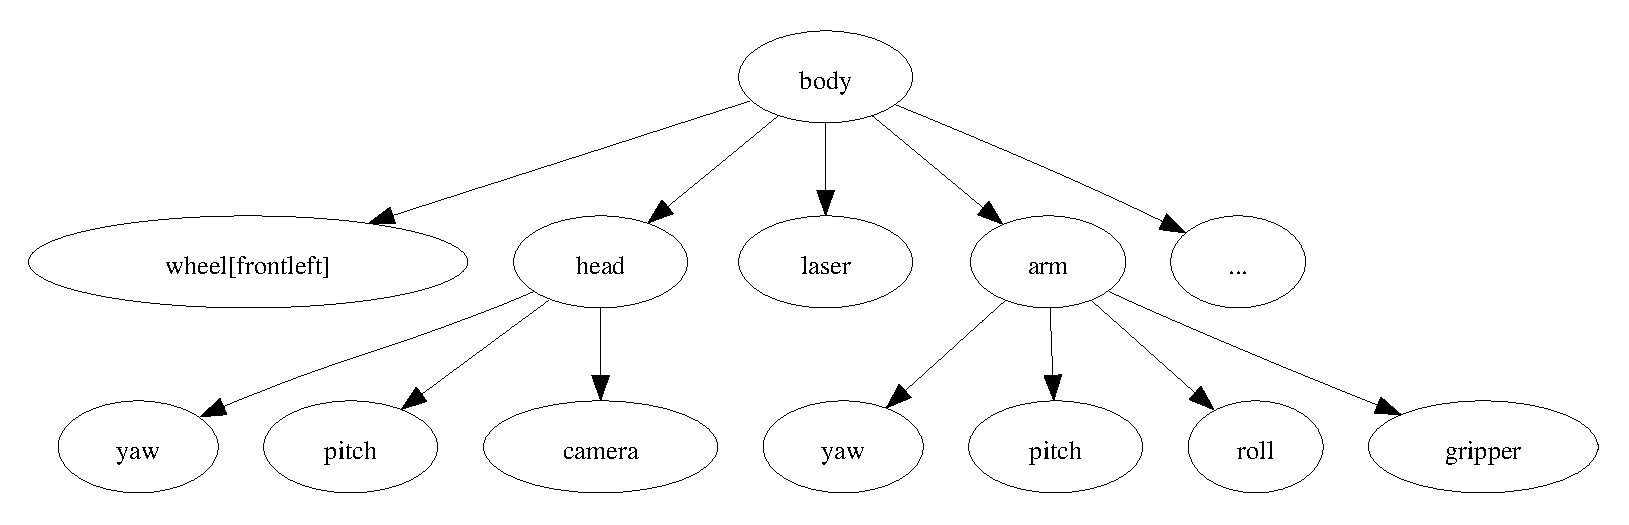
\includegraphics[width=.8\linewidth]{img/structure-tree-wheeled}
\end{center}

And here is another example for an humanoid robot:

\begin{center}
  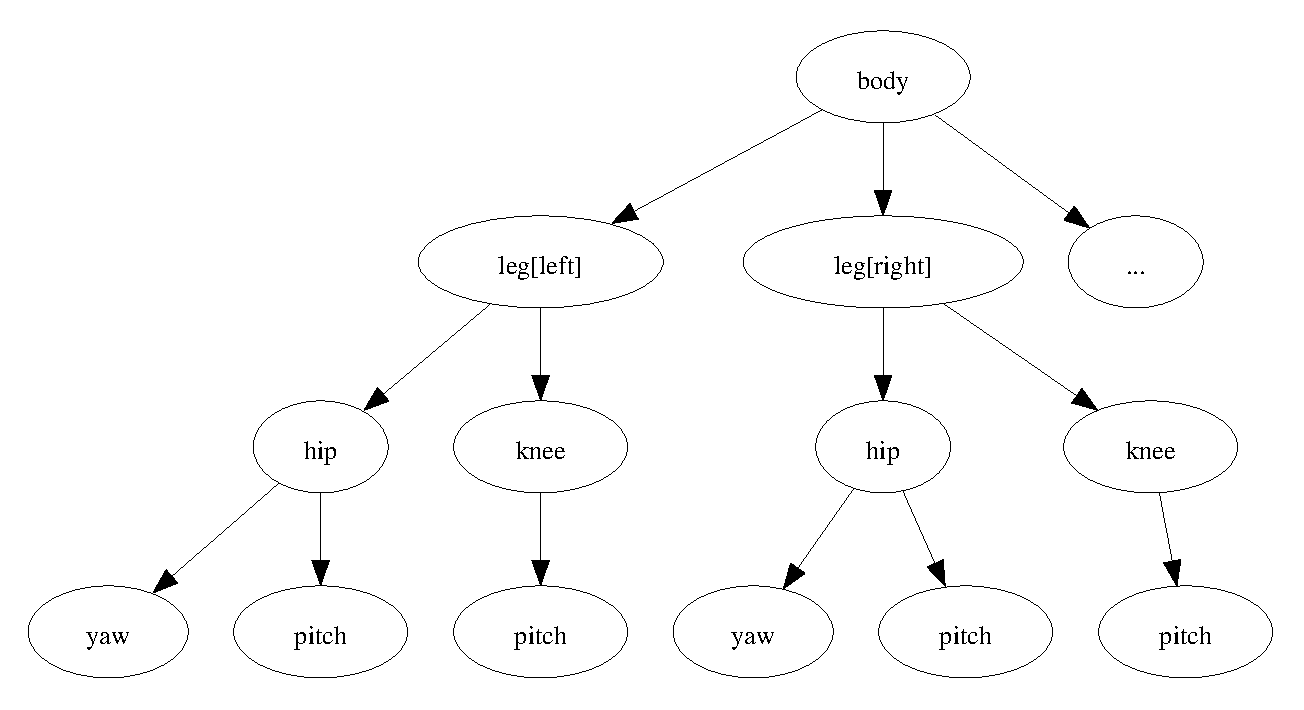
\includegraphics[width=.8\linewidth]{img/structure-tree-humanoid}
\end{center}

The leaves of the tree are called \textit{devices}, and they usually
match physical devices in the robot: motors, sensors, lights, camera,
etc. Inside \urbi, the various objects corresponding to the tree
components are accessed by following the path of objects inclusions,
like in the example below (shortcuts will be described later):

\begin{urbiunchecked}
body.leg[right].hip.tilt;
body.arm.grip;
body.laser;
// ...
\end{urbiunchecked}


The structure tree should not be mistaken for a representation of the
kinematics chain of the robot. The kinematics chain is built from a
subset of the devices corresponding to motor devices, and it
represents spatial connections between them. Except for these motor
devices, the structure tree components do not have a direct
counterpart in the kinematics chain, or, if they do, it is as a subset
of the kinematics chain (for example, \code{leg[right]} is a subset of the
whole kinematics chain).


The goal of this standard is to provide guidelines on how to define
the components and the structure tree, knowing the kinematics chain of
the robot.

\section{Frame of Reference}

In many cases, it will be necessary to refer to an absolute frame of
reference attached to the robot body. To avoid ambiguities, the
standard frame of reference will have the following definition:

\begin{center}
  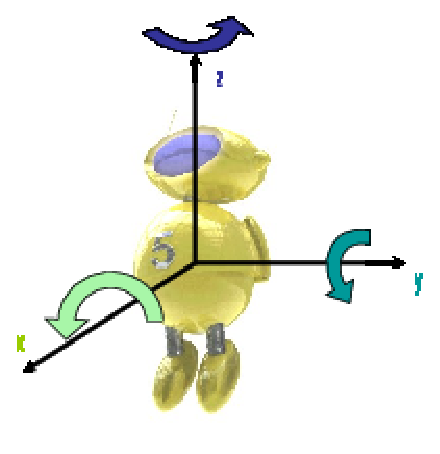
\includegraphics{img/reference-frame}
\end{center}

\begin{description}
\item[Origin] the center of mass of the robot
\item[X axis] oriented towards the front of the robot. If there is a
  camera, the front is defined by the default direction of the camera,
  otherwise the front will be seen as the natural frontal orientation
  for a mobile robot (the direction of ``forward'' movement). If the
  robot is not naturally oriented, the X axis will be chosen to match
  the main axis of symmetry of the robot body and it will be oriented
  towards the smallest side, typically the top of a cone for
  example. In case of a perfectly symmetrical body, the X axis can be
  chosen arbitrarily but a clear mark should be made visible on the
  robot body to indicate it.
\item[Z axis] oriented in the opposite direction from the gravity. If
  there is no gravity or natural up/down orientation in the
  environment or normal operation mode of the robot, the Z axis should
  be chosen in the direction of the main axis of symmetry in the
  orthogonal plane defined by the X axis, oriented towards the
  smallest side. In case of a perfectly symmetrical plane, the Z axis
  can be chosen arbitrarily but a clear mark should be made visible on
  the robot body to indicate it.
\item[Y axis] oriented to make a right-handed coordinate system.
\end{description}


The axes are oriented in a counter-clockwise direction, as depicted in
the illustration above.

\section{Component naming}

Each component A, which is a sub-component of component B has a name, distinct
from the name of all the other components at the same level.
This name is a generic designation of what A represents, such as ``leg''
,``head'', or ``finger''.

Using the correct name for each component is a critical part of this standard.
No formal rule can be given to find this name for any possible robot
configuration. However, this document includes a table covering many different
possible cases. We recommend that robot manufacturers pick from this table
the name that fits the most the description of their component.

\section{Localization}
When two identical components A1 and A2, such as the two legs of an humanoid
robots, are present in the same sub-component B, an extra node is inserted in
the hierarchy to differentiate them. This node is of the \code{Localizer} type,
and provides a \code{[]} operator, taking a \code{Localization} argument, used
to access each of the identical sub-components.
The \usdk provides an implementation for the \code{Localizer} and
\code{Localization} classes.
When possible, localization should be simple geometrical qualifier like
\textit{right}/\textit{center}/\textit{left},
\textit{front}/\textit{middle}/\textit{back} or
\textit{up}/\textit{in-between}/\textit{down}.
Note that ``right'' or ``front'' are
understood here from the point of view of a man standing and looking
in the direction of the X-axis of the robot, and \textit{up/pown}
matches the Z-axis, as depicted in the figure below:

\begin{center}
  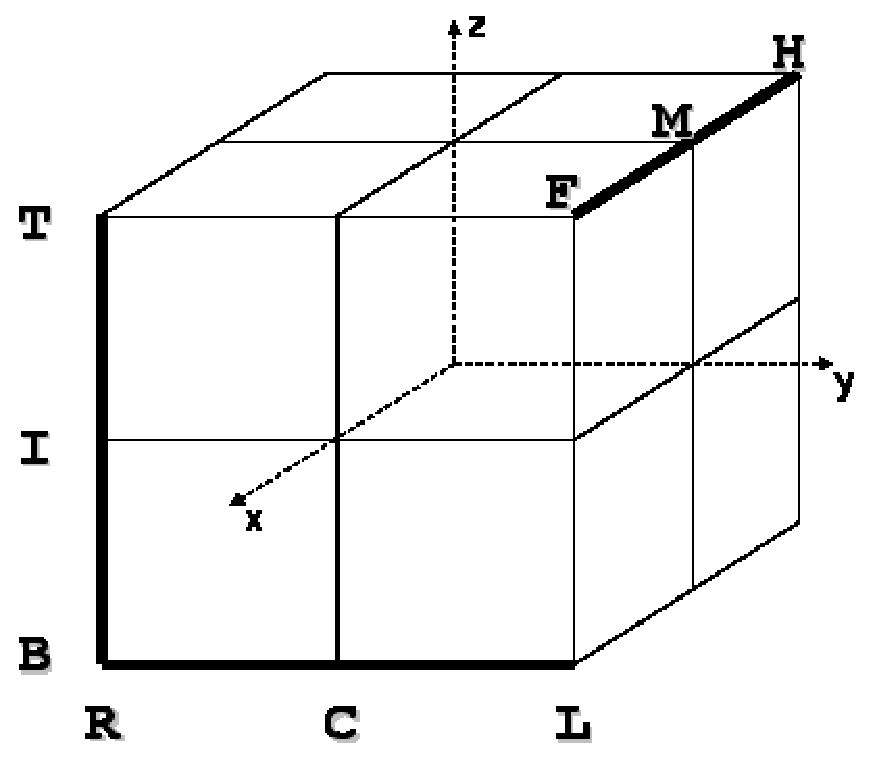
\includegraphics[width=.5\linewidth]{img/cube}
\end{center}

Several geometric qualifiers can be used at the same time to further
refine the position. In this case, multiple Localizer nodes are used.
As a convention, height information (U/I/D) comes first,
followed by depth information (F/M/H), and then side information (R/C/L).

\begin{urbiunchecked}
// Front-left wheel of a four-wheeled robot:
robot.body.wheel[front][left];
// Front laser of a robot equipped with multiple sonars:
robot.body.laser[front];
// Left camera from a robot with a stereo camera at the end of an arm:
robot.body.arm.camera[left];
// Top-left LED of the left eye.
robot.body.head.eye[left].led[up][left].val = 1;
// Touch sensor at the end of the front-left leg of a four-legged robot:
robot.body.leg[front][left].foot.touch;
\end{urbiunchecked}

You can further qualify a side+depth localization with an additional
F/B side information. This can be used in the typical layout below:

\begin{center}
  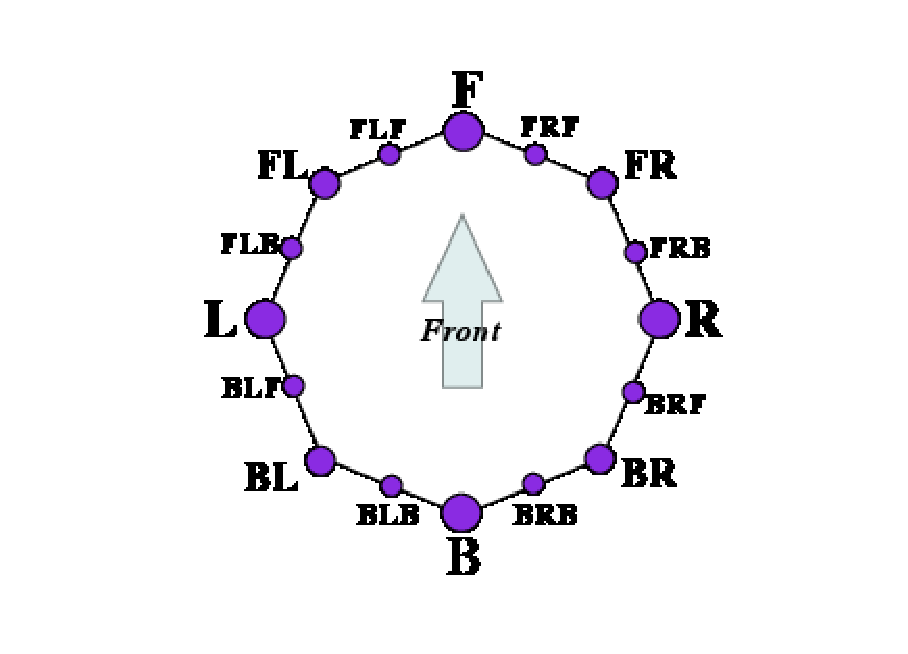
\includegraphics{img/localizer-multidim}
\end{center}

This dual positioning using side+depth can also be used to combine
side+height or height+depth information.

Layouts with a sequence of three or more identical components can use numbers
as their Localization, starting from 0.  The smaller the number, the closer to
the front, up, or left. For instance, an insectoid robot with 3 legs on each
side will use
\code{robot.body.leg[left][0]} to address the frontleft leg.

Layouts with identical components arranged in a circle can also use numeric
localization. The component with index 0 should be the uppermost, or front-most
if non applicable. Index should increase counterclockwise.

Some components like spines or tails are highly articulated with a set
of identical sub-components. When talking about these sub-components,
the above localization should be replaced by an array with a numbering
starting at 0. The smaller the number, the closer the sub-component is
to the robot main body. For surface-like sub-components, like skin
touch sensors, the array can be two dimensional.


Other possible localization for sensors are the X, Y and Z axis
themselves, like for example for an accelerometer or a gyro sensor,
available in each of the three directions.

\begin{urbiunchecked}
robot.body.accel[x]; // accelerometer in the x direction
\end{urbiunchecked}


Examples of component names including localization:

\begin{urbiunchecked}
leg[right], leg[left];
finger[right], finger[center], finger[left];      // three-finger hand
joint[0], joint[1] ... joint[5] // from tail
touch[478][124]                 // from skin
accel[x], accel[y], accel[z];         // typical accelerometer
gyro[x], gyro[y], gyro[z];            // typical gyro sensor
\end{urbiunchecked}

\section{Interface}
\label{sec:interface}

An ``interface'' describes some aspects of a type of device, by specifying the
slots and methods that implementations must provide. Each child node of
the component hierarchy should implement at least one interface.

For example, for a joint, we can have a ``Swivel'' interface, used to define
patella joints. For the robot body itself, we have a ``Mobile'' interface
describing mobile robots, which includes some standard way of
requesting a move forward, a turn, etc.

In short, interfaces are standard Urbi objects that components can inherit
from to declare that they have some functionalities.

The following pages describe a few of the most standard interfaces. Each
device in the component hierarchy which falls within the category of an
interface should implement it.

Each interface defines slots, which can be functions, events or plain data.
Some of those slots are optional: they are grayed and put around square
brackets in the following table.

\interface{Identity}

Contains information about the robot identity.

\begin{urbiscriptapi}
\item[type]%
  This describes the robot category among: humanoid, four-legged, wheeled,
  industrial arm. It gives a general idea of the robot family, but does not
  replace a more systematic probe of available services by investigating the
  list of attributes of the object.

\item[name]%
  Name of the robot.

\item[model] Model of the robot.

\item[serial] Serial number (if available).
\end{urbiscriptapi}


\interface{Network}

Contains information about the network identification of the robot.

\begin{urbiscriptapi}
\item[IP] IP address of the robot.
\end{urbiscriptapi}

\interface{Motor}

This interface is used to describe a generic motor controller.

\begin{urbiscriptapi}
\item[val] This slot is a generic pointer to a more specific slot describing
  the motor position, like \code{position} or \code{angle}, depending on the
  type of motor. It is mandatory in the Urbi Ready standard as a universal
  proxy to control an actuator. The more specific slot is described in a
  subclass of \code{Motor}.
\item[PGain?] Controls the P gain of the PID controller.
\item[IGain?] Controls the I gain of the PID controller.
\item[DGain?] Controls the D gain of the PID controller.
\end{urbiscriptapi}

\interface[Motor]{LinearMotor}


This interface is used to describe a linear motor controller.

A wheel can fall in this category, if the reported position is the distance
traveled by a point at the surface of the wheel.

\begin{urbiscriptapi}
\item[position] Position of the motor in meters.  Pointed to by the
  \code{val} slot.

\item[force] Intensity of the measured or estimated force applied on a
  linear motor.
\end{urbiscriptapi}

\interface[Motor]{LinearSpeedMotor}

Motor similar to \code{LinearMotor}, but controlled by its translation speed.

\begin{urbiscriptapi}
\item[speed] Translation speed in meters per second. Pointed to by the
  \code{val} slot.
\end{urbiscriptapi}


\interface[Motor]{RotationalMotor}


This interface is used to describe a position-controlled rotational motor
controller.

\begin{urbiscriptapi}
\item[angle] Angle of the motor in radian, modulo $2\pi$. Pointed to by the
  \code{val} slot.

\item[turn] Absolute angular position of the motor, expressed in number of
  turns.

\item[torque] Intensity of the measured or estimated torque applied on the
  motor.
\end{urbiscriptapi}

\interface[Motor]{RotationalSpeedMotor}

Interface describing a motor similar to \code{RotationalMotor} controlled
by its rotation speed.

\begin{urbiscriptapi}
\item[speed] Rotation speed in radians per second.
\end{urbiscriptapi}

\interface{Sensor}

This interface is used to describe a generic sensor.

\begin{urbiscriptapi}
\item[val] This slot is a generic pointer to a more specific slot describing
  the sensor value, like \code{distance} or \code{temperature}, depending on
  the type of sensor. It is mandatory in the Urbi Ready standard as a
  universal proxy to read a sensor. The more specific slot is described in a
  subclass of \code{Sensor}.
\end{urbiscriptapi}


\interface[Sensor]{DistanceSensor}

This interface is used to describe a distance sensor (infrared, laser,
ultrasonic...).

\begin{urbiscriptapi}
\item[distance] Measured distance expressed in meters.  Pointed to by the
  \code{val} slot.
\end{urbiscriptapi}


\interface[Sensor]{TouchSensor}

This interface is used to describe a touch pressure sensor (contact,
induction,...).

\begin{urbiscriptapi}
\item[pressure] Intensity of the pressure put on the touch sensor. Can be
  0/1 for simple buttons or expressed in Pascal units. Pointed to by the
  \code{val} slot.
\end{urbiscriptapi}


\interface[Sensor]{AccelerationSensor}

This interface is used to describe an accelerometer.

\begin{urbiscriptapi}
\item[acceleration] Acceleration expressed in $m/s^2$.  Pointed to by the
  \code{val} slot.
\end{urbiscriptapi}

\interface[Sensor]{GyroSensor}
This interface is used to describe an gyrometer.

\begin{urbiscriptapi}
\item[speed] Rotational speed in $\mathrm{rad}/s$.  Pointed to by the
  \code{val} slot.
\end{urbiscriptapi}

\interface[Sensor]{TemperatureSensor}
This interface is used to describe a temperature sensor.

\begin{urbiscriptapi}
\item[temperature] Measured temperature in Celsius degrees.  Pointed to by
  the \code{val} slot.
\end{urbiscriptapi}

\interface[Sensor]{Laser}
Interface for a scanning laser rangefinder, or other similar technologies.

\begin{urbiscriptapi}
\item[val] Last scan result. Can be either a list of ufloat, or a binary
  containing a packed array of doubles.

\item[angleMin] Start scan angle in radians, relative to the front of the
  device.

\item[angleMax] End scan angle in radians, relative to the front of the
  device.

\item[resolution] Angular resolution of the scan, in radians.

\item[distanceMin] Minimum measurable distance.

\item[distanceMax] Maximum measurable distance.

\item[rate?] Number of scans per second.
\end{urbiscriptapi}

Depending on the implementation, some of the parameters can be read-only, or
can only accept a few possible values. In that case it is up to the implementer
to select the closest possible value to what the user entered. It is the
responsibility of the user to read the parameter after setting it to check
what value will actually be used by the implementation.


\interface{Mobile}

Mobile robots all share this generic interface to provide high order
level motion control capabilities.

\begin{urbiscriptapi}
\item[go](<x>) Move approximately \var{x} meters forward if \var{x} is
  positive, backward otherwise.

\item[turn](<x>) Turn right approximately \var{x} radians.  \var{x} can be a
  positive or negative value.
\end{urbiscriptapi}

\interface{Tracker}

Camera-equipped robots can sometimes move the orientation of the field
of view horizontally and vertically, which is a very important feature
for many applications. In that case, this interface abstracts how such
motion can be achieved, whether it is done with a pan/tilt camera or
with whole body motion or a combination of both.

\begin{urbiscriptapi}
\item[yaw] Rotational articulation around the Z axis in the robot, expressed
  in radians.
\item[pitch] Rotational articulation around the Y axis in the robot,
  expressed in radians.
\end{urbiscriptapi}

\interface{VideoIn}

The VideoIn interface groups every information relative to cameras or any
image sensor.

\begin{urbiscriptapi}
\item[val] Image represented as a \code{Binary} value.
\item[xfov] The x field of view of the camera expressed in radians.
\item[yfov] The y field of view of the camera expressed in radians.

\item[height] Height of the image in the current resolution, expressed in
  pixels.

\item[width] Width of the image in the current resolution, expressed in
  pixels

\item[format?]
    Format of the image, expressed as an integer in the enum
    urbi::UImageFormat.  See below for more information.

\item[exposure?] Exposure duration, expressed in seconds. 0 if non
  applicable.

\item[wb?]  White balance (expressed with an integer value depending on the
  camera documentation). 0 if non applicable.

\item[gain?]  Camera gain amplification (expressed as a coefficient between
  0 and infinity). 1 if non applicable.

\item[resolution?]  Image resolution, expressed as an integer. 0 corresponds
  to the maximal resolution of the camera. Successive values correspond to
  all the supported image sizes in decreasing order.  Once modified, the
  effective resolution in X/Y can be checked with the width and height
  slots.

\item[quality?]  If the image is in the jpeg format, this slot sets the
  compression quality, from 0 (best compression, worst quality) to 100 (best
  quality, bigger image).
\end{urbiscriptapi}

The image sensor is expected to use the cheapest way in term of CPU and/or
energy consumption to produce images of the requested format.
Implementations linked to a physical image sensor do not have to implement
all the possible formats. In this case, the format closest to what was
requested must be used.
A generic image conversion object will be provided. In order to avoid
duplicate image conversions when multiple unrelated behaviors need the same
format, it is recommended that this object be instantiated in a slot of the
VideoIn object named after the format it converts to:
\begin{urbiunchecked}
if (!robot.body.head.camera.hasSlot("jpeg"))
{
  var robot.body.head.camera.jpeg =
    ImageConversion.new(robot.body.head.camera.getSlot("val"));
  robot.body.head.camera.jpeg.format = 3;
}
\end{urbiunchecked}

\interface{AudioOut}
The AudioOut interface groups every information relative to speakers.

\begin{urbiscriptapi}
\item[val] The speaker value, expressed as a binary, in the format given by
  the binary header during the assignment.

  Speakers are write-only devices, so there is not much sense in reading the
  content of this attribute. At best, it returns the remaining sound to be
  played if it is not over yet, but this is not a requirement.


\item[remain] The amount of time remaining to play in the speaker sound
  buffer (expressed in \textit{ms} as a default unit).


\item[playing] This is a Boolean value which is true when there is a sound
  currently playing (the buffer is not empty)%

\item[volume?] Volume of the play back, in decibels.
\end{urbiscriptapi}



\interface{AudioIn}

The AudioIn interface groups every information relative to microphones.

\begin{urbiscriptapi}
\item[val] Binary value corresponding to the sound heard, expressed in the
  current unit (wav, mp3...). The unit can be changed like any other regular
  unit in Urbi.

  The content is the sound heard by the microphone since the last update
  event.
\item[duration] Amount of sound in the val attribute, expressed in
  \textit{ms}.
\item[gain?] Microphone gain amplification (expressed between 0 and 1).
\end{urbiscriptapi}


\interface{BlobDetector}

Ball detectors, marker detectors and various feature-based detectors
should all share a similar interface. They extract a part of the image
that fits some criteria and define a \dfn{blob} accordingly. Here are
the typical slots expected:

\begin{urbiscriptapi}
\item[x] The x position of the center of the blob in the image

\item[y] The y position of the center of the blob in the image

\item[ratio] The size of the blob expressed as a normalized image size: 1 =
  full image, 0 = nothing.

\item[visible] A Boolean expressing whether there is a blob in the image or
  not (see \refSlot{threshold}).

\item[threshold] The minimum value of ratio to decide that the blob is
  visible.

\item[orientation?]  Angle of the main ellipsoid axis of the blob (0 =
  horizontal), expressed in radians.

\item[elongation?]  Ratio between the main and the second diameter of the
  blob enveloping ellipse.
\end{urbiscriptapi}

\interface{TextToSpeech}
Text to speech allows to read text using a speech synthesizer. Default
implementations should use the \code{speaker} component (or alias) as
their default sound output.

\begin{urbiscriptapi}
\item[lang?]  The language used, in international notation (fr, en, it…):
  ISO 639

\item[speed?]  How fast the voice should go.  A positive number, with 1
  standing for ``regular speed''.

\item[pitch?] Voice pitch.  A positive number, with 1 standing the regular
  pitch.

\item[gender?] Gender of the speaker (0:male/1:female).

\item[age?] Age of the speaker, if applicable.

\item[voice?]
    Most TTS engines propose several voices, this attribute allows picking
    one. It's a string identifier specific to the TTS developer.

\item[say](s) Speak the sentence given in parameter \var{s}.

\item[voicexml?](s) Speak the text \var{s} expressed as a VoiceXML string.

\item[script?](s) Speak the text \var{s} augmented by script markups (see
  specific Gostai documentation) to generate \urbi events.
\end{urbiscriptapi}


\interface{SpeechRecognizer}

Speech recognition allows to transform a stream of sound into a text
using various speech recognition algorithms. Implementations
should use the \code{micro} component as their default sound input.

\begin{urbiscriptapi}
\item[lang?]  The language used, in international notation (fr, en, it…):
  ISO 639.
\item[hear](s) This event has one parameter which is the string describing
  what the speech engine has recognized (can be a word or a sentence).
\end{urbiscriptapi}

\interface{Led}

Simple uni-color Led.

\begin{urbiscriptapi}
\item[val] Led intensity between 0 and 1.
\end{urbiscriptapi}


\interface[Led]{RGBLed}

Tri-color led.

\begin{urbiscriptapi}
\item[r] Intensity of the red component, between 0 and 1.
\item[g] Intensity of the green component, between 0 and 1.
\item[b] Intensity of the blue component, between 0 and 1.
\end{urbiscriptapi}

\interface{Battery}

Power source of any kind.

\begin{urbiscriptapi}
\item[remain] Estimation of the remaining energy between 0 and 1.
\item[capacity] Storage capacity in Amp.Hour.
\item[current] Current current consumption in Amp.
\item[voltage] Current voltage in Volt.
\end{urbiscriptapi}


\section{Standard Components}

Standard components correspond to components typically found in wheeled
robots, humanoid or animaloid robots, or in industrial arms. This section
provides a list of such components. Whenever possible, robots compatible with
the \gsrapi should name all the components in the hierarchy using this list.

\subsection{Yaw/Pitch/Roll orientation}
\label{sec:naming:ypr}

Note that \gsrapi considers the orientation to be a component name, and
not a localizer. So one would write \lstinline|head.yaw| and not
\lstinline|head.joint[yaw]| to refer to a rotational articulation of the head
around the Z axis.

It is not always clear which rotational direction corresponds to the
yaw, pitch or roll components (listed in the table below). This is a
quick guideline to help determine the proper association.

Let us consider the robot in its resting, most prototypical position,
like ``standing'' on two or four legs for a humanoid or animaloid, and
let all members ``naturally'' fall under gravity. When gravity has no
effect on a certain joint (because it is in the orthogonal plan to Z,
for example), the medium position between rangemin and rangemax should
be used. The body position achieved will be considered as a reference.
Then for each component that is described in terms of yaw/pitch/roll
sub-decomposition, the association will be as follow:

\begin{description}
\item[yaw] rotational articulation around the Z axis in the robot.
\item[pitch] rotational articulation around the Y axis in the robot.
\item[roll] rotational articulation around the X axis in the robot.
\end{description}

When there is no exact match with the X/Y/Z axis, the closest match, or
the default remaining available axis, should be selected to determine
the yaw/pitch/roll meaning.

\subsection{Standard Component List}
\label{sec:naming:components}

The following table summarizes the currently referenced standard
components, with a description of potential components that they could
be sub-component of, a description of potential components they may
contain, and a list of relevant interfaces. This table should be seen as a
quick reference guide to identify available components in a given
robot.

\newcommand{\component}[5]
{
  \lstindex{#1} &
  #5 &
  \code{#2} &
  \code{#3} &
  \code{#4}\\\hline
}

\tablehead{\hline
\textbf{Name} &
\textbf{Description} &
\textbf{Sub. of} &
\textbf{Contains} &
\textbf{Facets} \\\hline}
\begin{supertabular}{|m{.115\linewidth}|m{.45\linewidth}|*{4}{m{.12\linewidth}|}}
  \component{robot}{}{body}{Identity Network Mobile Tracker}{
    %%
    This is the main component that represents an abstraction of the
    robot, and the root node of the whole component hierarchy.
    %%
  }

  \component{body}{robot}{wheel arm leg neck head wheel tail skin torso
    \ldots}{}{
    %%
    This is the main component that contains every piece of hardware
    in the robot. This includes all primary kinematics sub-chains
    (arms, legs, neck, head, etc) and non-localized sensor arrays,
    typically body skin or heat detectors.  Localized sensors, like
    fingertips touch sensors, will typically be found attached to the
    finger component they belong and not directly to the body.
    %%
  }

  \component{wheel}{body}{}{Rotational\-Motor}{
    %%
    Wheel attached to its parent component.
    %%
  }
  \component{leg}{body}{hip knee ankle foot joint}{}{
    %%
    Legs are found in humanoid or animaloid robots and correspond to
    part of the kinematics chain that are attached to the main body by
    one extremity only and which do touch the ground in normal
    operation mode (unlike arms). A typical configuration for
    humanoids contains a hip, a knee and an ankle. If the leg is more
    segmented, the leg can be described with a simple array of joints.
    %%
  }

  \component{arm}{body}{shoulder elbow wrist hand grip joint}{}{
    %%
    Unlike legs, an arm's extremity does not always touch the ground
    in normal operating mode. This applies to humanoid robots or
    single-arm industrial robots. Arms supersede legs in the
    nomenclature: if a body part behaves alternatively like an arm and
    like a leg, it will be considered as an arm.
    %%
  }

  \component{shoulder}{arm}{yaw pitch roll}{}{
    %%
    The shoulder is the upper part of the arm. It can have one, two or
    three degrees of freedom and is the closest part of the arm
    relative to the body.
    %%
  }

  \component{elbow}{arm}{pitch}{}{
    %%
    Separates the upper arm and the lower arm, this is usually a
    single rotational axis.
    %%
  }

  \component{wrist}{arm}{yaw pitch roll}{}{
    %%
    Connects the hand and the lower part of the arm. Usually three
    degrees of freedom axis.
    %%
  }

  \component{hand}{arm}{finger}{}{
    %%
    The hand is an extension of the arm that usually holds
    fingers. It's not the wrist, which is articulated and between the
    arm and the hand.
    %%
  }

  \component{finger}{hand}{touch}{Motor}{
    %%
    Fingers are a series of articulated motors at the extremity of the
    arm, and connected to the hand. They are usually localized with
    arrays and/or lateral localization respective to the hand.
    %%
  }

  \component{grip}{arm hand}{touch}{Motor}{
    %%
    Simple two-fingers system.
    %%
  }

  \component{hip}{leg}{yaw pitch roll}{}{
    %%
    The hip is the upper part of the leg and connects it to the main
    body. It can have one, two or three degrees of freedom.
    %%
  }

  \component{knee}{leg}{pitch}{}{
    %%
    Separates the upper leg and the lower leg, this is usually a
    single rotational axis.
    %%
    }

  \component{ankle}{leg}{yaw pitch roll}{}{
    %%
    Connects the foot and the lower part of the leg. Usually three
    degrees of freedom axis.
    %%
    }

  \component{foot}{leg}{touch}{}{
    %%
    The foot is an extension of the leg that usually holds toes. It's
    not the ankle, which is articulated and between the leg and the
    foot. The foot can also contain touch sensors in simple
    configurations.
    %%
  }

  \component{toe}{foot}{touch}{Motor}{
    %%
    Like fingers, but attached to the foot.
    %%
  }

  \component{neck}{body}{yaw pitch roll}{}{
    %%
    The neck corresponds to a degree of freedom not part of the head,
    but relative to the rigid connection between the head and the main
    body.
    %%
  }

  \component{tail}{body}{joint}{}{
    %%
    A tail is a series of articulated motors at the back of the robot.
    %%
  }

  \component{head}{body neck}{camera mouth ear lip eye eyebrow}{}{
    %%
    The head main pivotal axis.
    %%
  }

  \component{mouth}{head}{lip}{Motor}{
    %%
    The robot mouth (open/close)
    %%
  }

  \component{ear}{head}{}{Motor}{
    %%
    Ears may have degrees of freedom in certain robots.
    %%
  }

  \component{joint}{tail arm leg lip}{}{Motor}{
    %%
    Generic articulation in the robot.
    %%
  }

  \component{yaw}{body neck knee ankle shoulder elbow wrist
    torso}{}{Rotational\-Motor Rotational\-Speed\-Motor}{
    %%
    Rotational articulation around the Z axis in the
    robot. See \autoref{sec:naming:ypr}.
    %%
  }

  \component{pitch}{body neck knee ankle shoulder elbow wrist
    torso}{}{Rotational\-Motor Rotational\-Speed\-Motor}{
    %%
    Rotational articulation around the Y axis in the
    robot.  See \autoref{sec:naming:ypr}.
    %%
  }

  \component{roll}{body neck knee ankle shoulder elbow wrist
    torso}{}{Rotational\-Motor Rotational\-Speed\-Motor}{
    %%
    Rotational articulation around the X axis in the robot. See
    \autoref{sec:naming:ypr}.
    %%
  }

  \component{x}{body arm}{}{Linear\-Motor Linear\-Speed\-Motor}{
    %%
    Translational movement along the X axis.
    %%
  }

  \component{y}{body arm}{}{Linear\-Motor Linear\-Speed\-Motor}{
    %%
    Translational movement along the Y axis.
    %%
  }

  \component{z}{body arm}{}{Linear\-Motor Linear\-Speed\-Motor}{
    %%
    Translational movement along the Z axis.
    %%
  }

  \component{lip}{mouth}{joint}{Motor}{
    %%
    Corresponds to animated lips.
    %%
  }

  \component{eye}{head}{camera}{}{
    %%
    Corresponds to the eyeball pivotal axis.
    %%
    }

  \component{eyebrow}{head}{joint}{Motor}{
    %%
    Some robots will have eyebrows with generally one or several
    degrees of freedom.
    %%
    }

  \component{torso}{body}{yaw pitch roll}{}{
    %%
    This corresponds to a pivotal or rotational axis in the middle of
    the main body.
    %%
    }

  \component{spine}{torso}{joint}{}{
    %%
    This is a more elaborated version of ``torso'', with a series of
    articulations to give several degrees of freedom in the back of
    the robot.
    %%
    }

  \component{clavicle}{body}{}{Motor}{
    %%
    This is not to be mixed up with the ``top of the arm'' body part. It
    is an independent degree of freedom that can be used to bring the
    two arms closer in a sort of ``shoulder raising'' movement.
    %%
    }

  \component{touch}{finger grip foot toe}{}{TouchSensor}{
    %%
      Touch sensor.
    %%
    }

  \component{gyro}{body}{}{GyroSensor}{
    %%
      Gyrometer sensor.
    %%
    }

  \component{accel}{body}{}{Accel\-eration\-Sensor}{
    %%
      Accelerometer sensor.
    %%
    }

  \component{camera}{head body}{}{VideoIn}{
    %%
    Camera sensor. If several cameras are available, localization
    shall apply; however there must always be an alias from
    \code{camera} to one of the effective cameras (like \code{cameraR}
    or \code{cameraL}).
    %%
    }

  \component{speaker}{head body}{}{AudioIn}{
    %%
    Speaker device. If several speakers are available, localization
    shall apply; however there must always be an alias from
    \code{speaker} to one of the effective speakers (like
    \code{speakerR} or \code{speakerL}).
    %%
    }

  \component{micro}{head body}{}{AudioOut}{
    %%
    Microphone devices. If several microphones are available,
    localization shall apply; however there must always be an alias
    from \code{micro} to one of the effective microphones (like
    \code{microR} or \code{microL}).
    %%
  }

  \component{speech}{robot}{}{Speech\-Recognizer}{
    %%
      Speech recognition component.
    %%
    }

  \component{voice}{robot}{}{TextTo\-Speech}{
    %%
      Voice synthesis component.
    %%
    }

\end{supertabular}



\section{Compact notation}

Components are usually identified with their full-length name, which is
the path to access them inside the structure tree. For convenience and
backward compatibility with pre-2.0 versions of \urbi, there is also a
compact notation available. We will describe here how to construct the
compact notation starting from the full name and the structure tree.

\tablehead{\hline
Full name &
Compact name\\\hline}
\begin{supertabular}{|m{9.008cm}|m{5.533cm}|}
\code{robot.body.armR.elbow} &
\code{elbowR} \\\hline
\code{robot.body.head.yaw} &
\code{headYaw} \\\hline
\code{robot.body.legL.knee.pitch} &
\code{kneeL} \\\hline
\code{robot.body.armR.hand.finger[3][2]} &
\code{fingerR[3][2]} \\\hline
\code{robot.body.armL.hand.fingerR} &
\code{fingerLR} \\\hline
\end{supertabular}

The rule is to move every localization qualifier at the end of the
compact notation, in the order where they appear in the full-length
name. The remaining component names should then be considered one by
one to see if they are needed to remove ambiguities. If they are not,
like typically the robot or body components which are shared with
almost every other full-length name, they can be ignored. If finally
several component names have to be kept, they should be separated by
using upper case letters for the first character instead of a dot, like
in Java-style notation.

\begin{example}[\code{robot.body.armL.hand.fingerR}]~\\
  \begin{enumerate}
  \item Move all localization at the end:
    \code{robot.body.arm.hand.fingerLR}
  \item The full name remaining is: \code{robot.body.arm.hand.finger}
  \item \code{finger} should be kept, \code{hand}, \code{arm},
    \code{body} and \code{robot} are not necessary since every
    finger component will always be attached only to a hand, itself
    attached to an arm and a body and a robot.
  \item The result is \code{fingerLR}
  \end{enumerate}
\end{example}


\begin{example}[\code{robot.body.head.yaw}]~\\
  \begin{enumerate}
  \item No localization to move
  \item \code{yaw} must be kept because \code{head} also have a
    \code{pitch} sub-component and
  \item \code{head} must also be kept to avoid ambiguity with other
    components having a \code{yaw} sub-component.
  \item The result is \code{headYaw}
  \end{enumerate}
\end{example}

\begin{example}[\code{robot.body.legL.knee.pitch}]~\\
  \begin{enumerate}
  \item Move all localization at the end:
    \code{robot.body.leg.knee.pitchL}
  \item \code{pitch} is not necessary because \code{knee} has only a
    \code{pitch}, so \code{knee} will be kept only
  \item The result is \code{kneeL}
  \end{enumerate}
\end{example}

\section{Support classes}
The \usdk provides a few support \us classes to help you build the component
hierarchy.  You can access to those classes by including the files
\file{urbi/naming-standard.u} and \file{urbi/component.h}.

\let\subsectionOrig\subsection
\let\subsection\subsectionObject

\subsection{Interface}

The \code{Interface} class contains \us objects for all the interfaces defined
in this document. Implementations must inherit from the correct interface.

\begin{urbiunchecked}
// Instantiate a camera.
var cam = myCamera.new();
// Make it inherit from VideoIn.
cam.addProto(Interface.VideoIn);
\end{urbiunchecked}

The \code{Interface.interfaces} method can be called to get a list of all
the interfaces an object implements.

\subsection{Component}

The \code{Component} class can be used to create intermediate nodes of the
hierarchy. It provides the following methods:

\begin{urbiscriptapi}

\item[addComponent](<name>)%
  Add a new sub-component to the current component. \var{name} can
  be the name of the new component to create, or an instance of
  \code{Component}.

\item[addDevice](<name>, <value>)%
  Add device \var{value} as sub-component, under the name \var{name}. The
  device must inherit from at least one Interface.

\item[makeCompactNames]%
  This function must be called once on the root node (\code{robot})
  after the hierarchy is completed.  It automatically computes the
  short name of all the devices, and insert them as slots of the
  \code{Global} object.

\item[dump]%
  Display a hierarchical view of the component hierarchy.

\item[flatDump]%
  Display all the devices in the hierarchy, sorted by the Interface
  they implement.
\end{urbiscriptapi}

\subsection{Localizer}

The \code{Localizer} class is a special type of \code{Component} that stores
other components based on their localization. It provides a \code{[]} operator
that takes a \code{Localization}, such as \lstinline|top,left,front|, and that
can be used to set and get the \code{Component} or device associated with
that \code{Localization}.

Note that the \code{[]} function is using a mechanisms to automatically look
for its argument as a slot of \code{Localizer}. As a consequence, you cannot
pass a variable to this function, but only one of the constant
\code{Localization}.
To pass a variable, use the \code{get(loc)} or the \code{set(loc, value)}
function.

The following example illustrates a typical instantiation sequence:

\begin{urbiunchecked}
// Create the top-level node.
var Global.robot = Component.new("robot");
robot.addComponent("head");
var cam = MyCamera.new;
cam.addProto(Interface.VideoIn);
robot.head.addDevice("camera", cam);
// Add two wheels
robot.addComponent(Localizer.new("wheel"));
robot.wheel[left] = MyWheel.new(0).addProto(Interface.RotationalMotor);
robot.wheel[right] = MyWheel.new(1).addProto(Interface.RotationalMotor);
// Implement the Mobile facet in urbiscript:
var robot.go = function(d)
{
  robot.wheel.val = robot.wheel.val + d / wheelRadius adaptive:1
};
var robot.turn = function(r)
{
  var v = r * wheelDistance / wheelRadius;
  robot.wheel[left].val = robot.wheel[left].val + v adaptive:1 &
  robot.wheel[right].val = robot.wheel[right].val - v adaptive:1
};
robot.addProto(Interface.Mobile);
robot.makeCompactNames;
// Let us see the result:
robot.flatDump;
[00010130] *** Mobile: robot
[00010130] *** RotationalMotor: wheelL wheelR
[00010130] *** VideoIn: camera
\end{urbiunchecked}

%% Restore the definition of \section.
\let\subsection\subsectionOrig

%%% Local Variables:
%%% mode: latex
%%% TeX-master: "../urbi-sdk"
%%% ispell-dictionary: "american"
%%% ispell-personal-dictionary: "../urbi.dict"
%%% fill-column: 76
%%% End:


%%% Local Variables:
%%% mode: latex
%%% TeX-master: "../urbi-sdk"
%%% ispell-dictionary: "american"
%%% ispell-personal-dictionary: "../urbi.dict"
%%% fill-column: 76
%%% End:


\part{References and Index}
\label{part:ref}

\phantomsection % otherwise hyperlinks to previous chapter.
\addcontentsline{toc}{chapter}{\indexname}
\printindex


\end{document}

% printing, operators, waituntil

% LocalWords:  Urbi monomethods netcat cosinus timestamp subscopes subscope lst
% LocalWords:  getSlot setSlot updateSlot slotNames removeSlot uid arg ok ko ss
% LocalWords:  elt baz quux FIXME getslot lookup protos proto addProto asString
% LocalWords:  removeProto locateSlot locateslot lhs evalArgAt evalArgs ary
% LocalWords:  mytag timeOut myEvent
